\chapter{Monte Carlo as a Research Instrument: Observing the CMB}\label{ch:08}
\providecommand{\EightANside}{}\renewcommand{\EightANside}{256}
\providecommand{\EightANpix}{}\renewcommand{\EightANpix}{786432}
\providecommand{\EightAPixSide}{}\renewcommand{\EightAPixSide}{13.7}
\providecommand{\EightAOmegaPix}{}\renewcommand{\EightAOmegaPix}{1.598\times10^{-5}}
\providecommand{\EightAFwhm}{}\renewcommand{\EightAFwhm}{30}
\providecommand{\EightASigmaBeam}{}\renewcommand{\EightASigmaBeam}{12.7}
\providecommand{\EightADepth}{}\renewcommand{\EightADepth}{200}
\providecommand{\EightASigmaPix}{}\renewcommand{\EightASigmaPix}{14.6}
\providecommand{\EightANell}{}\renewcommand{\EightANell}{3.38\times10^{-3}}
\providecommand{\EightALmax}{}\renewcommand{\EightALmax}{512}
\providecommand{\EightALmaxSim}{}\renewcommand{\EightALmaxSim}{767}
\providecommand{\EightARmsSky}{}\renewcommand{\EightARmsSky}{108}
\providecommand{\EightARmsBeamed}{}\renewcommand{\EightARmsBeamed}{86}
\providecommand{\EightARmsNoise}{}\renewcommand{\EightARmsNoise}{14.6}
\providecommand{\EightARmsObs}{}\renewcommand{\EightARmsObs}{88}
\providecommand{\EightABeamMaxDev}{}\renewcommand{\EightABeamMaxDev}{8\times10^{-7}}
\providecommand{\EightABeamHpDev}{}\renewcommand{\EightABeamHpDev}{0}
\providecommand{\EightABeamDevFive}{}\renewcommand{\EightABeamDevFive}{0.2}
\providecommand{\EightABeamDevTen}{}\renewcommand{\EightABeamDevTen}{0.6}
\providecommand{\EightALHalf}{}\renewcommand{\EightALHalf}{224}
\providecommand{\EightALHalfFormula}{}\renewcommand{\EightALHalfFormula}{225}
\providecommand{\EightABlmax}{}\renewcommand{\EightABlmax}{0.165}
\providecommand{\EightAPlmax}{}\renewcommand{\EightAPlmax}{0.827}
\providecommand{\EightAPlTwoFiveSix}{}\renewcommand{\EightAPlTwoFiveSix}{0.954}
\providecommand{\EightATlmaxSq}{}\renewcommand{\EightATlmaxSq}{0.0186}
\providecommand{\EightACholSix}{}\renewcommand{\EightACholSix}{0.80}
\providecommand{\EightALikeDaysTwoFiveSix}{}\renewcommand{\EightALikeDaysTwoFiveSix}{21}
\providecommand{\EightALikeYrFiveTwelve}{}\renewcommand{\EightALikeYrFiveTwelve}{4}
\providecommand{\EightALikeYrPlanck}{}\renewcommand{\EightALikeYrPlanck}{1.5\times10^{4}}
\providecommand{\EightAShtTwoFiveSix}{}\renewcommand{\EightAShtTwoFiveSix}{0.02}
\providecommand{\EightAShtPlanck}{}\renewcommand{\EightAShtPlanck}{9}
\providecommand{\EightAMemTwoFiveSix}{}\renewcommand{\EightAMemTwoFiveSix}{4.9}
\providecommand{\EightAMemPlanck}{}\renewcommand{\EightAMemPlanck}{20266}
\providecommand{\EightALeq}{}\renewcommand{\EightALeq}{436}
\providecommand{\EightANoverSlmax}{}\renewcommand{\EightANoverSlmax}{3.0}
\providecommand{\EightANoverSthree}{}\renewcommand{\EightANoverSthree}{0.05}
\providecommand{\EightAFracErrCVlmax}{}\renewcommand{\EightAFracErrCVlmax}{4.4}
\providecommand{\EightAFracErrNlmax}{}\renewcommand{\EightAFracErrNlmax}{18}
\providecommand{\EightAFracErrNthree}{}\renewcommand{\EightAFracErrNthree}{6.0}
\providecommand{\EightAFracErrCVthree}{}\renewcommand{\EightAFracErrCVthree}{5.8}
\providecommand{\EightAPnegSeven}{}\renewcommand{\EightAPnegSeven}{46}
\providecommand{\EightANoverSseven}{}\renewcommand{\EightANoverSseven}{246}
\providecommand{\EightAFracErrNseven}{}\renewcommand{\EightAFracErrNseven}{9.33}
\providecommand{\EightAPnegLeq}{}\renewcommand{\EightAPnegLeq}{4\times10^{-38}}
\providecommand{\EightANsim}{}\renewcommand{\EightANsim}{2000}
\providecommand{\EightAMinutes}{}\renewcommand{\EightAMinutes}{6}
\providecommand{\EightASecPerSky}{}\renewcommand{\EightASecPerSky}{0.19}
\providecommand{\EightANbins}{}\renewcommand{\EightANbins}{21}
\providecommand{\EightAChiAuto}{}\renewcommand{\EightAChiAuto}{20.5}
\providecommand{\EightAPAuto}{}\renewcommand{\EightAPAuto}{0.49}
\providecommand{\EightAChiCross}{}\renewcommand{\EightAChiCross}{15.5}
\providecommand{\EightAPCross}{}\renewcommand{\EightAPCross}{0.79}
\providecommand{\EightAMaxAbsBias}{}\renewcommand{\EightAMaxAbsBias}{0.16}
\providecommand{\EightATypBiasErr}{}\renewcommand{\EightATypBiasErr}{0.04}
\providecommand{\EightANoSubBiasLast}{}\renewcommand{\EightANoSubBiasLast}{278}
\providecommand{\EightANoSubBiasFirst}{}\renewcommand{\EightANoSubBiasFirst}{0.16}
\providecommand{\EightAPixForgotLast}{}\renewcommand{\EightAPixForgotLast}{-31}
\providecommand{\EightAMisLast}{}\renewcommand{\EightAMisLast}{-5.4}
\providecommand{\EightAMisPredLast}{}\renewcommand{\EightAMisPredLast}{-5.5}
\providecommand{\EightANlRatio}{}\renewcommand{\EightANlRatio}{1.0001}
\providecommand{\EightANlRatioErr}{}\renewcommand{\EightANlRatioErr}{0.0001}
\providecommand{\EightACrossRatioLmax}{}\renewcommand{\EightACrossRatioLmax}{1.25}
\providecommand{\EightACrossRatioMCLast}{}\renewcommand{\EightACrossRatioMCLast}{1.24}
\providecommand{\EightAVarRatio}{}\renewcommand{\EightAVarRatio}{1.001}
\providecommand{\EightAVarRatioErr}{}\renewcommand{\EightAVarRatioErr}{0.001}
\providecommand{\EightAVarChi}{}\renewcommand{\EightAVarChi}{498}
\providecommand{\EightAVarDof}{}\renewcommand{\EightAVarDof}{511}
\providecommand{\EightAVarPval}{}\renewcommand{\EightAVarPval}{0.65}
\providecommand{\EightAVarFracOut}{}\renewcommand{\EightAVarFracOut}{5.1}
\providecommand{\EightASpreadOne}{}\renewcommand{\EightASpreadOne}{3.2}
\providecommand{\EightACVRatio}{}\renewcommand{\EightACVRatio}{1.001}
\providecommand{\EightALHalfNoiseVar}{}\renewcommand{\EightALHalfNoiseVar}{386}
\providecommand{\EightANoiseFracLmax}{}\renewcommand{\EightANoiseFracLmax}{56}
\providecommand{\EightACrossFracLmax}{}\renewcommand{\EightACrossFracLmax}{37}
\providecommand{\EightAKSthree}{}\renewcommand{\EightAKSthree}{0.09}
\providecommand{\EightAKSthirty}{}\renewcommand{\EightAKSthirty}{0.19}
\providecommand{\EightAKSleq}{}\renewcommand{\EightAKSleq}{0.64}
\providecommand{\EightAKSlmax}{}\renewcommand{\EightAKSlmax}{0.10}
\providecommand{\EightASkewThree}{}\renewcommand{\EightASkewThree}{1.07}
\providecommand{\EightASkewThreeTh}{}\renewcommand{\EightASkewThreeTh}{1.07}
\providecommand{\EightASnrPeakEll}{}\renewcommand{\EightASnrPeakEll}{314}
\providecommand{\EightASnrPeak}{}\renewcommand{\EightASnrPeak}{16.6}
\providecommand{\EightASnrEq}{}\renewcommand{\EightASnrEq}{10.4}
\providecommand{\EightASnrCumLmax}{}\renewcommand{\EightASnrCumLmax}{280}
\providecommand{\EightASnrCVLmax}{}\renewcommand{\EightASnrCVLmax}{363}
\providecommand{\EightASnrCumSim}{}\renewcommand{\EightASnrCumSim}{281}
\providecommand{\EightASnrCVSim}{}\renewcommand{\EightASnrCVSim}{543}
\providecommand{\EightALNinety}{}\renewcommand{\EightALNinety}{378}
\providecommand{\EightASigAmc}{}\renewcommand{\EightASigAmc}{0.00364}
\providecommand{\EightASigAth}{}\renewcommand{\EightASigAth}{0.00358}
\providecommand{\EightASigAerr}{}\renewcommand{\EightASigAerr}{1.6}
\providecommand{\EightAMeanA}{}\renewcommand{\EightAMeanA}{1.00004}
\providecommand{\EightAMeanAerr}{}\renewcommand{\EightAMeanAerr}{0.00008}
\providecommand{\EightAInhContrast}{}\renewcommand{\EightAInhContrast}{5}
\providecommand{\EightAInhVmax}{}\renewcommand{\EightAInhVmax}{1.81}
\providecommand{\EightAInhVmin}{}\renewcommand{\EightAInhVmin}{0.36}
\providecommand{\EightAInhVsq}{}\renewcommand{\EightAInhVsq}{1.230}
\providecommand{\EightAInhBias}{}\renewcommand{\EightAInhBias}{0.9999}
\providecommand{\EightAInhBiasErr}{}\renewcommand{\EightAInhBiasErr}{0.0001}
\providecommand{\EightAInhVarNoise}{}\renewcommand{\EightAInhVarNoise}{1.055}
\providecommand{\EightAInhVarNoisePred}{}\renewcommand{\EightAInhVarNoisePred}{1.053}
\providecommand{\EightAInhVarTotLmax}{}\renewcommand{\EightAInhVarTotLmax}{1.024}
\providecommand{\EightAInhVarTotPredLmax}{}\renewcommand{\EightAInhVarTotPredLmax}{1.030}
\providecommand{\EightAInhVarTotLow}{}\renewcommand{\EightAInhVarTotLow}{1.000}
\providecommand{\EightASigBin}{}\renewcommand{\EightASigBin}{1.68}
\providecommand{\EightANTenPct}{}\renewcommand{\EightANTenPct}{51}
\providecommand{\EightANOnePermil}{}\renewcommand{\EightANOnePermil}{281}
\providecommand{\EightARelErrN}{}\renewcommand{\EightARelErrN}{6.9}
\providecommand{\EightARelErrNval}{}\renewcommand{\EightARelErrNval}{107}
\providecommand{\EightARelErrNth}{}\renewcommand{\EightARelErrNth}{6.9}
\providecommand{\EightAKnoxWinv}{}\renewcommand{\EightAKnoxWinv}{7.33}
\providecommand{\EightAKnoxRms}{}\renewcommand{\EightAKnoxRms}{95}
\providecommand{\EightAKnoxSnrPix}{}\renewcommand{\EightAKnoxSnrPix}{4.3}
\providecommand{\EightAKnoxNsim}{}\renewcommand{\EightAKnoxNsim}{300}
\providecommand{\EightAKnoxNside}{}\renewcommand{\EightAKnoxNside}{512}
\providecommand{\EightAKnoxLmax}{}\renewcommand{\EightAKnoxLmax}{1000}
\providecommand{\EightAKnoxMinutes}{}\renewcommand{\EightAKnoxMinutes}{5.0}
\providecommand{\EightAKnoxROursTwenty}{}\renewcommand{\EightAKnoxROursTwenty}{1.000}
\providecommand{\EightAKnoxROursForty}{}\renewcommand{\EightAKnoxROursForty}{0.999}
\providecommand{\EightAKnoxRKnoxTwenty}{}\renewcommand{\EightAKnoxRKnoxTwenty}{1.053}
\providecommand{\EightAKnoxRKnoxForty}{}\renewcommand{\EightAKnoxRKnoxForty}{1.013}
\providecommand{\EightAKnoxRHiTwenty}{}\renewcommand{\EightAKnoxRHiTwenty}{1.25}
\providecommand{\EightAKnoxLgoodTwenty}{}\renewcommand{\EightAKnoxLgoodTwenty}{801}
\providecommand{\EightAKnoxLgoodForty}{}\renewcommand{\EightAKnoxLgoodForty}{429}
\providecommand{\EightAKnoxMCerr}{}\renewcommand{\EightAKnoxMCerr}{4.1}
\providecommand{\EightAKnoxBeats}{}\renewcommand{\EightAKnoxBeats}{yes}
\providecommand{\EightAKnoxShortMs}{}\renewcommand{\EightAKnoxShortMs}{23}
\providecommand{\EightAKnoxShortRatio}{}\renewcommand{\EightAKnoxShortRatio}{0.999}
\providecommand{\EightAKnoxBiasLow}{}\renewcommand{\EightAKnoxBiasLow}{0.07}
\providecommand{\EightAHivRfirst}{}\renewcommand{\EightAHivRfirst}{1.85}
\providecommand{\EightAHivRsixteenMin}{}\renewcommand{\EightAHivRsixteenMin}{0.989}
\providecommand{\EightAHivRsixteenMax}{}\renewcommand{\EightAHivRsixteenMax}{1.098}
\providecommand{\EightAHivRsixteen}{}\renewcommand{\EightAHivRsixteen}{1.023}
\providecommand{\EightAHivRexact}{}\renewcommand{\EightAHivRexact}{1.003}
\providecommand{\EightAHivRexactMin}{}\renewcommand{\EightAHivRexactMin}{0.987}
\providecommand{\EightAHivRexactMax}{}\renewcommand{\EightAHivRexactMax}{1.040}
\providecommand{\EightAHivRsixteenErr}{}\renewcommand{\EightAHivRsixteenErr}{1.6}
\providecommand{\EightAHivNbins}{}\renewcommand{\EightAHivNbins}{10}
\providecommand{\EightAHivLfour}{}\renewcommand{\EightAHivLfour}{388}
\providecommand{\EightAHivFfull}{}\renewcommand{\EightAHivFfull}{0.072}
\providecommand{\EightAHivFmc}{}\renewcommand{\EightAHivFmc}{0.072}
\providecommand{\EightAHivNmc}{}\renewcommand{\EightAHivNmc}{0.071}
\providecommand{\EightAHivFresc}{}\renewcommand{\EightAHivFresc}{0.53}
\providecommand{\EightAHivFratio}{}\renewcommand{\EightAHivFratio}{1.00}
\providecommand{\EightAHivFratioErr}{}\renewcommand{\EightAHivFratioErr}{0.01}
\providecommand{\EightAHivNratio}{}\renewcommand{\EightAHivNratio}{0.99}
\providecommand{\EightAHivNratioErr}{}\renewcommand{\EightAHivNratioErr}{0.01}
\providecommand{\EightAHivSDratio}{}\renewcommand{\EightAHivSDratio}{1.01}
\providecommand{\EightAHivSDratioErr}{}\renewcommand{\EightAHivSDratioErr}{0.01}
\providecommand{\EightAHivMethratio}{}\renewcommand{\EightAHivMethratio}{0.98}
\providecommand{\EightAHivMethratioErr}{}\renewcommand{\EightAHivMethratioErr}{0.01}
\providecommand{\EightAHivSDmc}{}\renewcommand{\EightAHivSDmc}{7.2}
\providecommand{\EightAHivSDth}{}\renewcommand{\EightAHivSDth}{7.1}
\providecommand{\EightAHivMethmc}{}\renewcommand{\EightAHivMethmc}{6.6}
\providecommand{\EightAHivMethth}{}\renewcommand{\EightAHivMethth}{6.8}
\providecommand{\EightAHivNDfrac}{}\renewcommand{\EightAHivNDfrac}{0.68}
\providecommand{\EightAHivKSchi}{}\renewcommand{\EightAHivKSchi}{0.09}
\providecommand{\EightAHivKSgauss}{}\renewcommand{\EightAHivKSgauss}{1\times10^{-5}}
\providecommand{\EightAScaleTwoFiveSix}{}\renewcommand{\EightAScaleTwoFiveSix}{0.04}
\providecommand{\EightAScaleFiveTwelve}{}\renewcommand{\EightAScaleFiveTwelve}{0.24}
\providecommand{\EightAScaleTenTwentyFour}{}\renewcommand{\EightAScaleTenTwentyFour}{1.2}
\providecommand{\EightAScaleTwentyFortyEight}{}\renewcommand{\EightAScaleTwentyFortyEight}{10}
\providecommand{\EightAScaleSkySec}{}\renewcommand{\EightAScaleSkySec}{19}
\providecommand{\EightAScaleHours}{}\renewcommand{\EightAScaleHours}{5}
\providecommand{\EightAScaleMapGB}{}\renewcommand{\EightAScaleMapGB}{0.40}
\providecommand{\EightAScaleDiskGB}{}\renewcommand{\EightAScaleDiskGB}{403}
\providecommand{\EightAScaleSpecMB}{}\renewcommand{\EightAScaleSpecMB}{60}
\providecommand{\EightAScaleModeFrac}{}\renewcommand{\EightAScaleModeFrac}{4.2}
\providecommand{\EightAScaleSNRloss}{}\renewcommand{\EightAScaleSNRloss}{4.9}
\providecommand{\EightAScaleMCerrTwoK}{}\renewcommand{\EightAScaleMCerrTwoK}{1.6}
\providecommand{\EightAScaleMCerrThree}{}\renewcommand{\EightAScaleMCerrThree}{4.1}
\providecommand{\EightAPivRhoFive}{}\renewcommand{\EightAPivRhoFive}{-0.74}
\providecommand{\EightAPivRhoTwo}{}\renewcommand{\EightAPivRhoTwo}{-0.99}
\providecommand{\EightAPivRhoTwoTrans}{}\renewcommand{\EightAPivRhoTwoTrans}{-0.99}
\providecommand{\EightAPivKdec}{}\renewcommand{\EightAPivKdec}{0.083}
\providecommand{\EightAPivKdecFromTwo}{}\renewcommand{\EightAPivKdecFromTwo}{0.083}
\providecommand{\EightAPivLdec}{}\renewcommand{\EightAPivLdec}{1155}
\providecommand{\EightAPivKdecMarg}{}\renewcommand{\EightAPivKdecMarg}{0.091}
\providecommand{\EightAPivRhoFiveMarg}{}\renewcommand{\EightAPivRhoFiveMarg}{-0.21}
\providecommand{\EightAPivRhoTwoMarg}{}\renewcommand{\EightAPivRhoTwoMarg}{-0.81}
\providecommand{\EightAPivKdecCV}{}\renewcommand{\EightAPivKdecCV}{0.030}
\providecommand{\EightAPivLdecCV}{}\renewcommand{\EightAPivLdecCV}{416}
\providecommand{\EightAPivRhoTwoCV}{}\renewcommand{\EightAPivRhoTwoCV}{-0.98}
\providecommand{\EightAPivLdecApprox}{}\renewcommand{\EightAPivLdecApprox}{972}
\providecommand{\EightAPivDstar}{}\renewcommand{\EightAPivDstar}{13.87}
\providecommand{\EightAPivLfive}{}\renewcommand{\EightAPivLfive}{694}
\providecommand{\EightAPivLtwo}{}\renewcommand{\EightAPivLtwo}{28}
\providecommand{\EightAPivSigNsFive}{}\renewcommand{\EightAPivSigNsFive}{0.0025}
\providecommand{\EightAPivSigAFive}{}\renewcommand{\EightAPivSigAFive}{0.0017}
\providecommand{\EightAPivSigATwo}{}\renewcommand{\EightAPivSigATwo}{0.0094}
\section*{Where this chapter is going}
\label{8a:sec:roadmap}

A Boltzmann code such as CAMB turns six cosmological numbers into an angular power
spectrum $\Cell$ (\cref{ch:T1}). That spectrum describes the \emph{ensemble} of skies the
theory could have produced. A telescope gives us one of those skies, and not even all of it:
it sees the sky through a beam that blurs it, stores it in pixels that average it, adds
detector noise to every pixel, and, once the Galaxy is cut away, sees only part of it. Each of
these steps changes the numbers we compute from the map. In \cref{ch:07} the spectrum
estimator $\Chat$ was computed on perfect, complete skies, and everything about its sampling
distribution was known in closed form: it is unbiased, it is a scaled $\chi^2_{2\ell+1}$
variable, and its variance is the cosmic variance $2\Cell^2/(2\ell+1)$. What survives of those
statements when the sky is observed by a real instrument? Monte Carlo simulation answers it.

In the pipeline of the book (physical model $\to$ field $\to$ what matters $\to$ summary
$\to$ sampling distribution $\to$ inference) the problem sits on one arrow: finding the
sampling distribution of the summary $\Chat$ under realistic observation. The beam and the
noise come first, on the full sky, where every answer can still be derived by hand. There
the simulations \emph{verify} known formulas, and the same machine is tested and trusted.
The mask comes next: it couples multipoles, correlates their errors and bends the
distribution of $\Chat$ away from any formula, and the simulations become the research
instrument (\cref{8a:fig:roadmap}). The output, a mean, a covariance and a distribution
shape for $\Chat$, is exactly what the likelihood of \cref{ch:09}, the Fisher forecast of
\cref{ch:10} and the topological summaries of \cref{ch:12} need.

\begin{figure}[htbp]
\centering
\begin{tikzpicture}[
  bx/.style={draw=accent,thick,rounded corners=2pt,fill=ideabg,font=\small,
             minimum height=10mm,align=center,text width=27mm},
  rb/.style={bx,draw=bdryred!80!black},
  gb/.style={bx,draw=tangentgreen!80!black},
  flow/.style={->,thick,accent}]
  \node[bx] (cl)  at (0,0)    {fiducial $\Cell$\\ (CAMB)};
  \node[bx] (sky) at (3.6,0)  {simulated skies\\ Gaussian $\alm$};
  \node[bx] (ins) at (7.2,0)  {instrument: beam,\\ pixels, noise};
  \node[bx] (est) at (10.8,0) {estimator $\Chat$\\ on each sky};
  \node[gb,text width=31mm] (fs)  at (8.9,-2.6) {full sky: bias, variance, shape known exactly\\[1pt]
     {\footnotesize\color{tangentgreen!60!black}simulation verifies}};
  \node[rb,text width=31mm] (ms)  at (12.4,-2.6) {mask: coupled,\\ correlated $\ell$'s\\[1pt]
     {\footnotesize\color{bdryred!80!black}simulation is the instrument}};
  \node[bx,text width=50mm] (use) at (10.65,-5.4) {likelihood, Fisher, topology\\ (Ch.\,\ref{ch:09}, \ref{ch:10}, \ref{ch:12})};
  \draw[flow] (cl) -- (sky); \draw[flow] (sky) -- (ins); \draw[flow] (ins) -- (est);
  \draw[flow] (est.south) -- ++(0,-0.5) -| (fs.north);
  \draw[flow] (est.south) -- ++(0,-0.5) -| (ms.north);
  \draw[flow] (fs.south) -- (fs.south |- use.north);
  \draw[flow] (ms.south) -- (ms.south |- use.north);
\end{tikzpicture}
\caption{The research problem. A fiducial spectrum is turned into many
simulated skies, each is observed by a model of the instrument, and the spectrum is
estimated on each. On the full sky (green) the statistics of the estimator follow from a
short derivation, and the simulations check it. Once the sky is masked (red) no formula is
exact, and the simulations are the only way to the mean, the covariance and the shape of
the distribution that the later chapters feed into a likelihood.}
\label{8a:fig:roadmap}
\end{figure}

\section{The research problem}
\label{8a:sec:problem}

Picture the data as they arrive. A detector sweeps across the sky and records a voltage
many times per second. Every sample is the temperature of a small patch of sky, averaged
over the response pattern of the telescope, plus noise from the detector and its
electronics. Months of samples are binned into a map of a few million pixels. A theorist,
meanwhile, has run CAMB and holds a curve $\Cell$. The question is how to put the map and the
curve on the same plot, and how big the error bars on that plot really are. Answering it
for the cosmic microwave background (CMB) is the research problem that organises everything below:

\begin{framing}[The research problem]
A theoretical CMB power spectrum $\Cell$, obtained from a fiducial cosmological model,
describes the ensemble-averaged statistics of the CMB sky. In practice, however, CMB
observations provide only a finite and potentially incomplete realization of this random
field. Sky masks, instrumental noise, beam effects, and other observational limitations
modify the statistical properties of the quantities extracted from the map.

The problem is to use Monte Carlo simulations of CMB skies generated from a fiducial
theoretical power spectrum to investigate how these observational effects influence the
statistical properties of CMB power-spectrum estimators. In particular, we seek to
determine the sampling distribution, bias, variance, and covariance of the recovered
spectrum and to assess the validity of commonly used analytical approximations for these
quantities.

The study will begin with the full-sky Gaussian case, for which the statistical properties
of $\Chat$ are known analytically, and then introduce partial-sky coverage through
realistic or controlled masks. The simulated realizations will be used to quantify the
resulting mode coupling and correlations between multipoles, and to determine how these
effects depend on the sky fraction, mask geometry, and multipole range.

The central computational question is therefore:
\begin{quote}
\textbf{How does incomplete and imperfect observation of the CMB alter the statistical
information contained in the measured angular power spectrum, and how accurately can these
effects be characterized using Monte Carlo simulations?}
\end{quote}
\end{framing}

The statement mixes several questions, and each needs a different tool. Before any
equation it helps to say them one at a time, in words, in the order in which they depend on
each other. The first is physical: what exactly does the instrument do to the sky? Only
when that is written down as a model can we ask what it does to the \emph{average} of the
estimator (does $\Chat$ still centre on $\Cell$?), then to its \emph{scatter} (how wide is the
spread over skies, and are neighbouring multipoles correlated?), and then to the
\emph{shape} of its distribution (is it still a scaled $\chi^2$, or close enough to a
Gaussian?). The last two questions are about the method itself: do the quick formulas that
everyone uses survive the comparison with simulations, and how many simulations does it take
to know?

In order, the questions are:
\begin{enumerate}
  \item What does the instrument do to the sky? (A beam, a pixel window, noise, a mask: the
        observation model.)
  \item Does the estimator still average to the true $\Cell$? If not, by how much is it
        off, and can the offset be removed? (Bias.)
  \item How much does it scatter from sky to sky, and do the errors at different
        multipoles move together? (Variance and covariance.)
  \item What is the full shape of its distribution? (The sampling distribution: the
        likelihood of \cref{ch:09} needs it, not just its width.)
  \item Are the standard analytic shortcuts, such as the Knox formula with a sky fraction
        $\fsky$, accurate, and where do they fail?
  \item How many simulated skies are needed to answer 2--5 to a given precision?
\end{enumerate}

On the full sky with a beam and noise, questions 1--4 have exact answers, which we derive below. That makes the full sky the place to build the simulation machine and to
check, number by number, that it reproduces what we already know. A machine that has passed
that test can then be trusted where the answers are not known.

\subsection{Why we do not simply maximise the likelihood}
\label{8a:sec:why-not-ml}

The procedure of \cref{ch:03} for finding an estimator starts from the likelihood: write
the probability of the data given the parameter, maximise it, read the error bar off its
curvature. For a CMB map the data model is
\begin{equation}
  \data = \mathsf A\,\bm s + \bm n ,
  \label{8a:eq:hobson-model}
\end{equation}
where $\bm s$ is the sky in pixels, the matrix $\mathsf A$ applies the beam and the
pointing, and $\bm n$ is Gaussian noise with covariance matrix $\mathsf N$
\srcref{HobsonBMC}{(10.8)--(10.9)}. Here the observed outcome is the whole map and the
hypotheses are the possible spectra $\Cell$; each spectrum is judged by how plausible the
random sky-plus-noise fluctuation it would need to produce this particular map is, the reading
set out for a single multipole in \cref{8a:sec:ml}. The sky is a Gaussian random field whose pixel covariance
$\mathsf S(\Cell)$ is fixed by the spectrum, and the noise is independent of it, so the map is
Gaussian with covariance $\mathsf S+\mathsf N$, the sum of the two covariances. Its density is the
multivariate Gaussian of \cref{ch:02},
$(2\pi)^{-N_{\rm pix}/2}\det(\mathsf S+\mathsf N)^{-1/2}\exp[-\frac12\data\T(\mathsf S+\mathsf N)^{-1}\data]$,
and minus twice its logarithm, read as a function of $\Cell$, is
\begin{equation}
  -2\ln\Like(\Cell)=\data\T(\mathsf S+\mathsf N)^{-1}\data+\ln\det(\mathsf S+\mathsf N)+\text{const}
  \label{8a:eq:pixel-like}
\end{equation}
\srcref{HobsonBMC}{(10.23)}, \cite{Efstathiou2004}.

What does maximising this over $\Cell$ give? Write $\mathsf C\equiv\mathsf S+\mathsf N$ for the
total covariance. The covariance of the sky between two pixels is a sum over $\ell$ of $\Cell$
times a fixed angular pattern (\cref{ch:07}), so $\mathsf S$ is linear in the spectrum,
$\mathsf S=\sum_\ell\Cell\,\mathsf S_\ell$, where $\mathsf S_\ell\equiv\partial\mathsf S/\partial\Cell$ is
the pixel covariance that one unit of $\Cell$ produces. Two matrix rules do the
differentiation: the derivative of an inverse,
$\partial\mathsf C^{-1}=-\mathsf C^{-1}(\partial\mathsf C)\,\mathsf C^{-1}$, and the derivative of a
log-determinant, $\partial\ln\det\mathsf C=\tr\bigl(\mathsf C^{-1}\partial\mathsf C\bigr)$. With
$\partial\mathsf C/\partial\Cell=\mathsf S_\ell$ and the shorthand
$\mathsf E_\ell\equiv\mathsf C^{-1}\mathsf S_\ell\,\mathsf C^{-1}$,
\begin{align}
  \frac{\partial\ln\Like}{\partial\Cell}
  &\eqby{1}\frac12\Bigl[\data\T\mathsf E_\ell\,\data-\tr\bigl(\mathsf C^{-1}\mathsf S_\ell\bigr)\Bigr]
   \eqby{2}\frac12\Bigl[\data\T\mathsf E_\ell\,\data-\tr\bigl(\mathsf E_\ell\mathsf N\bigr)\Bigr]
     -\sum_{\ell'}F_{\ell\ell'}C_{\ell'} ,
  \nonumber\\
  \widehat C_\ell^{\,\rm QML}
  &\eqby{3}\frac12\sum_{\ell'}\bigl(F^{-1}\bigr)_{\ell\ell'}
   \Bigl[\data\T\mathsf E_{\ell'}\,\data-\tr\bigl(\mathsf E_{\ell'}\mathsf N\bigr)\Bigr].
  \label{8a:eq:qml}
\end{align}
\begin{explain}
  \item Differentiate \eqref{8a:eq:pixel-like} with the two rules and multiply by $-\tfrac12$.
  \item Insert $\mathsf C\,\mathsf C^{-1}$ into the trace, $\tr(\mathsf C^{-1}\mathsf S_\ell)=\tr(\mathsf E_\ell\mathsf C)$,
        and split $\mathsf C=\sum_{\ell'}C_{\ell'}\mathsf S_{\ell'}+\mathsf N$. The sky part gives
        $\sum_{\ell'}C_{\ell'}\tr(\mathsf E_\ell\mathsf S_{\ell'})=2\sum_{\ell'}F_{\ell\ell'}C_{\ell'}$, with
        $F_{\ell\ell'}=\frac12\tr(\mathsf C^{-1}\mathsf S_\ell\mathsf C^{-1}\mathsf S_{\ell'})$ the Fisher
        matrix of the spectrum (\cref{ch:03}).
  \item Set the slope to zero and solve for the $C_{\ell'}$. The matrices $\mathsf E_\ell$ and
        $F$ still contain $\Cell$, so they are evaluated at a fiducial spectrum, and the solution is
        one Newton step from it; repeating the step with the result as the new fiducial converges to
        the maximum.
\end{explain}
The estimator \eqref{8a:eq:qml} is \emph{quadratic in the data}, because the data enter only
through $\data\T\mathsf E_\ell\data$. Read from the inside out, it weights the map by the inverse
covariance, correlates it with the pattern $\mathsf S_\ell$ that a change in one $\Cell$ would
produce, subtracts the part of that correlation the noise alone would give, $\tr(\mathsf E_\ell\mathsf N)$,
and normalises by the Fisher matrix. This is the \newterm{quadratic maximum-likelihood} (QML) estimator
\cite{Efstathiou2004}. On a complete sky with uniform noise every matrix is diagonal in the
harmonic coordinates (the real numbers $u_k$ of \eqref{8a:eq:u-def}): $\mathsf C$ has $V_\ell=T_\ell^2\Cell+N_\ell$ on the $\nu=2\ell+1$ modes of each $\ell$,
and $\mathsf S_\ell$ has $T_\ell^2$ on them. Then $\data\T\mathsf E_\ell\data=T_\ell^2\nu\,\widehat C^{\,\rm obs}_\ell/V_\ell^2$,
$\tr(\mathsf E_\ell\mathsf N)=T_\ell^2\nu N_\ell/V_\ell^2$ and $F_{\ell\ell}=\nu T_\ell^4/2V_\ell^2$, and
\eqref{8a:eq:qml} collapses to $(\widehat C^{\,\rm obs}_\ell-N_\ell)/T_\ell^2$, with the fiducial
$V_\ell$ cancelling: the average of
$|\alm|^2$ over $m$ with the noise subtracted, which \cref{8a:sec:ml} obtains directly.

The trouble is the size of the matrices. Every evaluation of \eqref{8a:eq:pixel-like} needs
the inverse and the determinant of an $N_{\rm pix}\times N_{\rm pix}$ matrix, which costs of
order $N_{\rm pix}^3$ operations and $8N_{\rm pix}^2$ bytes of memory
\srcref{HobsonBMC}{p.~238}, \srcref{Hivon}{§1}.

\paragraph{Example: how long is one likelihood evaluation?}
On an ordinary desktop computer, the Cholesky factor of a $6000\times6000$
covariance takes $\EightACholSix$\,s (\cref{8a:fig:cost}). The cost grows as $N^3$, so for
the $N_{\rm pix}=\EightANpix$ pixels of a HEALPix map at $N_{\rm side}=256$ the same operation
takes about $\EightALikeDaysTwoFiveSix$ days, and the matrix alone occupies
$\EightAMemTwoFiveSix$\,TB. At $N_{\rm side}=512$ it is about $\EightALikeYrFiveTwelve$
years. At $N_{\rm side}=2048$, the resolution of the Planck maps, it is
$\EightALikeYrPlanck$ years for a single evaluation, and a parameter fit needs tens of
thousands of them. A spherical-harmonic transform of the same Planck-size map, which is all
the simple estimator needs, takes about $\EightAShtPlanck$\,s, because on the iso-latitude
HEALPix grid its cost grows only as $N_{\rm pix}^{3/2}$ \srcref{Hivon}{§2.2},
\cite{Gorski2005}.

\begin{figure}[htbp]
\centering
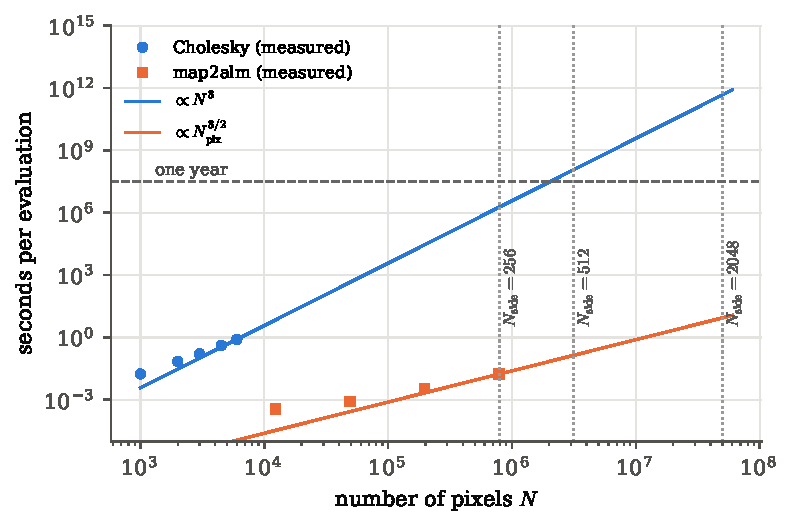
\includegraphics[width=10cm]{figures/ch08/cost_scaling.pdf}
\caption{Time for one evaluation of the exact pixel likelihood (blue: a Cholesky
factorisation, which grows as $N^3$) and for one spherical-harmonic transform (orange,
growing as $N_{\rm pix}^{3/2}$). Points are measured, lines are extrapolations from the
largest measured size. The dotted verticals mark three HEALPix resolutions, the dashed
horizontal one year.}
\label{8a:fig:cost}
\end{figure}

\paragraph{Example: when is the cheap estimator as good as the expensive one?}
Two limits are known exactly \cite{Efstathiou2004}. When the signal dominates the noise,
the cheap estimator with equal weight on every pixel is statistically equivalent to the
maximum-likelihood one. When the noise dominates and is uncorrelated between pixels, the
cheap estimator with each pixel weighted by its inverse noise variance is mathematically
identical to it. Between the two limits, and with a mask, it loses some information, and
the loss has to be measured.

So the field took a different road, and the recipe of \cref{ch:03} already contains it: its
step~5, for problems whose likelihood cannot be evaluated. Choose a statistic that is cheap
and sensitive to $\Cell$: the average of $|\alm|^2$ over $m$, computed directly on the
observed map, which on a cut sky is called the \newterm{pseudo-$\Cell$}
\srcref{Hivon}{(13)}. Then simulate many skies, pass each through the same instrument and
the same analysis, and read off the mean, the scatter and the shape of the statistic from
the simulations. The statistic is suboptimal, but its bias is calibrated out and its error
bar is honest. Hivon and collaborators named the method after this calibration step:
MASTER, the Monte Carlo Apodised Spherical Transform EstimatoR \srcref{Hivon}{§1}.

\begin{figure}[htbp]
\centering
\begin{tikzpicture}[
  bx/.style={draw=accent,thick,rounded corners=2pt,fill=ideabg,font=\small,
             minimum height=11mm,align=center,text width=25mm},
  nt/.style={font=\footnotesize,align=center,text width=27mm,softgray!40!black},
  flow/.style={->,thick,accent}]
  \node[bx] (tod) at (0,0)    {time-ordered\\ data $d_t$};
  \node[bx] (map) at (3.7,0)  {map $\data$};
  \node[bx] (cl)  at (7.4,0)  {spectrum $\Chat$};
  \node[bx] (par) at (11.1,0) {parameters $\params$};
  \node[nt,above=2mm of tod] {detector noise,\\ $1/f$ drifts, scan};
  \node[nt,above=2mm of map] {beam, pixels,\\ residual noise};
  \node[nt,above=2mm of cl]  {noise bias, mask,\\ correlations};
  \node[nt,above=2mm of par] {likelihood\\ (Ch.\,9, 10)};
  \draw[flow] (tod) -- (map); \draw[flow] (map) -- (cl); \draw[flow] (cl) -- (par);
  \draw[decorate,decoration={brace,mirror,amplitude=5pt},thick,fibreorange]
       ([yshift=-3mm]map.south west) -- ([yshift=-3mm]cl.south east);
  \node[font=\footnotesize,fibreorange!80!black] at (5.55,-1.25) {where beam, pixels, noise and mask act};
\end{tikzpicture}
\caption{The CMB analysis as a chain of compressions \srcref{HobsonBMC}{§10.2}. Each step
keeps the information the next one needs, and each adds its own complications (grey). The
bracket marks the middle link: how the beam, the pixels and the noise of the map, and the
mask, change the statistics of the spectrum computed from it.}
\label{8a:fig:hierarchy}
\end{figure}

The chain of \cref{8a:fig:hierarchy} is called a hierarchical model
\srcref{HobsonBMC}{§10.2}: the timestream is compressed into a map, the map into a
spectrum, the spectrum into parameters, and each step only needs the output of the one
before. Making the map from the timestream is a least-squares problem of its own; for white
noise it reduces to averaging the samples that fall in each pixel, which divides the noise
variance by the number of hits \srcref{HobsonBMC}{(10.14)--(10.15)}. Real detector noise has
extra power at low frequencies ($1/f$ noise), which leaves stripes along the scan and has to
be filtered out \srcref{Hivon}{§2.1}, \srcref{HobsonBMC}{p.~234}. We start from the map and
assume the noise left in it is Gaussian and uncorrelated between pixels, with a variance
that may change from pixel to pixel. Everything that this simplification leaves out
(filtering, correlated noise, asymmetric beams) is exactly the kind of effect that real
pipelines handle by putting it into the simulations \srcref{Hivon}{§3.2--3.3}.
\section{What the instrument does to the sky}
\label{8a:sec:model}

A radio telescope pointed in direction $\hat{\bm n}$ does not measure the temperature at
the single point $\hat{\bm n}$. Its optics collect radiation from a small cone around
$\hat{\bm n}$, weighted by the \newterm{beam}: the response pattern of the telescope, the
same object an astronomer calls the point-spread function. What it records is therefore a
weighted average of the sky. The recorded averages are then binned into pixels, which
averages them a second time over the area of each pixel. Finally every pixel carries noise
from the detector. The three steps act at different places, and the order matters: the beam
and the pixels act on the sky, while the noise is added afterwards and is blurred by
neither.

\begin{workdef}[observation model of a temperature map]
The \newterm{observed map} is
\begin{equation}
  d_p=\int_{S^2} b\bigl(\hat{\bm n}_p\cdot\hat{\bm n}'\bigr)\,s(\hat{\bm n}')\,\dd\Omega' + n_p
  \equiv (B\circledast s)(\hat{\bm n}_p)+n_p ,
  \label{8a:eq:obs-model}
\end{equation}
where $s(\hat{\bm n})$ is the sky temperature fluctuation in $\mu$K, $\hat{\bm n}_p$ is the
centre of pixel $p$, $b$ is the beam \unpack{the weight given to the sky at angle
$\gamma$ from the pointing, a function of $\cos\gamma=\hat{\bm n}_p\cdot\hat{\bm n}'$ only for a
circular beam}, normalised as $\int b\,\dd\Omega=1$, and $n_p$ is the noise of pixel $p$
\unpack{Gaussian, mean zero, variance $\sigma_p^2$, independent of the sky and of the noise in
every other pixel}. The pixel average is included as one more smoothing of $s$.
\emph{Operationally:} to simulate an observation, smooth the simulated sky with the beam and
the pixel, then add one independent Gaussian number to each pixel.
\end{workdef}

This is the model \eqref{8a:eq:hobson-model} written out for a single detector with a
circular beam, after the timestream has been turned into a map
\srcref{HobsonBMC}{(10.6)--(10.7)}. The same structure, data equal smoothed model plus
noise, appears in the cosmology notes as $\data=\bm s(\params)+\bm n$ with the beam inside
$\bm s$ (see the cosmology notes).

\subsection{A beam multiplies each multipole by a number}
\label{8a:sec:beam}

Smoothing is a convolution, and on a line a convolution becomes a multiplication in Fourier
space. The sphere has the same property, with spherical harmonics in place of Fourier
modes and with one condition: the smoothing kernel must depend only on the angle between the
two directions. To see it, expand the beam, a function of $x=\cos\gamma$ on $[-1,1]$, in
Legendre polynomials,
\begin{equation}
  b(x)=\sum_{\ell=0}^{\infty}\frac{2\ell+1}{4\pi}\,B_\ell\,P_\ell(x),
  \qquad
  B_\ell=2\pi\int_{-1}^{1}b(x)\,P_\ell(x)\,\dd x .
  \label{8a:eq:beam-legendre}
\end{equation}
The formula for $B_\ell$ follows by multiplying the expansion by $P_{\ell'}$ and integrating,
using $\int_{-1}^1P_\ell P_{\ell'}\,\dd x=2\delta_{\ell\ell'}/(2\ell+1)$. The coefficient
$B_0=2\pi\int b\,\dd x=\int b\,\dd\Omega=1$ is the normalisation: the beam does not change the
mean of the sky. Now smooth a sky $s=\sum_{\ell m}\alm Y_{\ell m}$ (\cref{ch:07}):
\begin{align}
  (B\circledast s)(\hat{\bm n})
  &\eqby{1}\int\sum_{\ell}\frac{2\ell+1}{4\pi}B_\ell\,P_\ell(\hat{\bm n}\cdot\hat{\bm n}')\,s(\hat{\bm n}')\,\dd\Omega' \nonumber\\
  &\eqby{2}\sum_{\ell}B_\ell\sum_{m=-\ell}^{\ell}Y_{\ell m}(\hat{\bm n})\int Y^*_{\ell m}(\hat{\bm n}')\,s(\hat{\bm n}')\,\dd\Omega' \nonumber\\
  &\eqby{3}\sum_{\ell m}\bigl(B_\ell\,\alm\bigr)\,Y_{\ell m}(\hat{\bm n}) .
  \label{8a:eq:convolution}
\end{align}
\begin{explain}
  \item Insert the Legendre expansion \eqref{8a:eq:beam-legendre} of the beam.
  \item The addition theorem $P_\ell(\hat{\bm n}\cdot\hat{\bm n}')=\frac{4\pi}{2\ell+1}\sum_m
        Y_{\ell m}(\hat{\bm n})Y^*_{\ell m}(\hat{\bm n}')$ (\cref{ch:07}); the factors $(2\ell+1)/4\pi$ cancel.
  \item The remaining integral is the definition of the harmonic coefficient $\alm$ of $s$.
\end{explain}

\begin{keyidea}[The convolution theorem on the sphere]
A circular beam multiplies every harmonic coefficient of the sky by a number that depends
on $\ell$ only: $\alm\to B_\ell\,\alm$. The beam does not mix different $(\ell,m)$, so the
smoothed sky is still statistically isotropic, with power spectrum $B_\ell^2\,\Cell$.
\end{keyidea}

The last statement follows from $\langle|B_\ell\alm|^2\rangle=B_\ell^2\langle|\alm|^2\rangle=
B_\ell^2\Cell$. In the cosmology notes the same factor is called the window function,
$W_\ell=B_\ell^2$ (see the cosmology notes); we keep $B_\ell$ because it is the factor that
multiplies $\alm$. A beam that is not circular has a kernel that depends on more than the
angle between the two directions, and then it does mix the $m$'s
\srcref{HobsonBMC}{p.~232}, \srcref{Hivon}{§3.6}.

\paragraph{The Gaussian beam.}
Most telescope main lobes are close to a two-dimensional Gaussian of width $\sigma_b$,
\begin{equation}
  b(\theta)=\frac{1}{2\pi\sigma_b^2}\,e^{-\theta^2/2\sigma_b^2},
  \qquad
  \sigma_b=\frac{\rm FWHM}{\sqrt{8\ln2}}\approx\frac{\rm FWHM}{2.355},
  \label{8a:eq:gauss-beam}
\end{equation}
where $\theta$ is the angle from the pointing and FWHM is the full width at half maximum
\unpack{the angular diameter of the circle on which the beam has fallen to half its peak}.
The relation between FWHM and $\sigma_b$ comes from setting $e^{-\theta^2/2\sigma_b^2}=1/2$
at $\theta={\rm FWHM}/2$, which gives ${\rm FWHM}^2/(8\sigma_b^2)=\ln 2$. Since the beam is
small, $\sin\theta\approx\theta$ and the normalisation is that of a flat two-dimensional
Gaussian. Its $B_\ell$ follows from \eqref{8a:eq:beam-legendre} with $x=\cos\theta$. For the
low multipoles, where $\ell\sigma_b\ll1$, expand $P_\ell$ around $x=1$:
\begin{align}
  B_\ell
  &\eqby{1}2\pi\int_0^{\pi}b(\theta)\,P_\ell(\cos\theta)\,\sin\theta\,\dd\theta \nonumber\\
  &\eqby{2}2\pi\int_0^{\infty}b(\theta)\Bigl[1-\frac{\ell(\ell+1)}{2}\,\frac{\theta^2}{2}\Bigr]\theta\,\dd\theta \nonumber\\
  &\eqby{3}1-\frac{\ell(\ell+1)}{4}\,\langle\theta^2\rangle_b \nonumber\\
  &\eqby{4}1-\frac{\ell(\ell+1)\,\sigma_b^2}{2} .
  \label{8a:eq:beam-small}
\end{align}
\begin{explain}
  \item Change variable $x=\cos\theta$, $\dd x=-\sin\theta\,\dd\theta$.
  \item Taylor expansion $P_\ell(\cos\theta)\approx P_\ell(1)+P_\ell'(1)(\cos\theta-1)$ with
        $P_\ell(1)=1$, $\cos\theta-1\approx-\theta^2/2$, and $P'_\ell(1)=\ell(\ell+1)/2$. The
        last value follows from Legendre's equation $(1-x^2)P''_\ell-2xP'_\ell+\ell(\ell+1)P_\ell=0$
        evaluated at $x=1$, where the first term vanishes. Also $\sin\theta\approx\theta$, and the
        upper limit can be moved to $\infty$ because the beam is negligible far from its centre.
  \item The first term is the normalisation $2\pi\int b\,\theta\,\dd\theta=1$. The second is
        the mean of $\theta^2$ over the beam, $\langle\theta^2\rangle_b\equiv2\pi\int\theta^2 b\,\theta\,\dd\theta$.
  \item For a two-dimensional Gaussian, $\theta^2=x^2+y^2$ with $x$ and $y$ independent, each of
        variance $\sigma_b^2$, so $\langle\theta^2\rangle_b=2\sigma_b^2$.
\end{explain}
Equation \eqref{8a:eq:beam-small} is the first-order expansion of
$e^{-\ell(\ell+1)\sigma_b^2/2}$, and the cosmology notes reach the same expansion for the
window function, $W_\ell\approx1-\sigma_b^2\ell(\ell+1)$. At high $\ell$ the flat-sky limit
fixes the full shape: on a small patch, $\ell$ becomes the length of a two-dimensional wave
vector, and the Fourier transform of a two-dimensional Gaussian is a Gaussian,
\begin{equation}
  \tilde b(\bm\ell)=\int\frac{e^{-(x^2+y^2)/2\sigma_b^2}}{2\pi\sigma_b^2}\,
  e^{-i(\ell_xx+\ell_yy)}\,\dd x\,\dd y
  =e^{-\ell_x^2\sigma_b^2/2}\,e^{-\ell_y^2\sigma_b^2/2}=e^{-\ell^2\sigma_b^2/2},
  \label{8a:eq:beam-flat}
\end{equation}
each factor being the familiar one-dimensional result obtained by completing the square.
The formula that joins both limits is the one used everywhere,
\begin{equation}
  B_\ell=\exp\Bigl[-\frac{\ell(\ell+1)\,\sigma_b^2}{2}\Bigr]
  \label{8a:eq:beam}
\end{equation}
\cite{Knox1995}, and it is what \pyname{healpy.gauss_beam} returns. Is it exact? The
function \pyname{gaussian_beam_exact} in \pyname{code/ch08/lib_cmbsim.py} evaluates the
Legendre integral \eqref{8a:eq:beam-legendre} numerically, with $P_\ell$ from Bonnet's
recursion $(\ell+1)P_{\ell+1}=(2\ell+1)xP_\ell-\ell P_{\ell-1}$. For a $30'$ beam the two
agree to $\EightABeamMaxDev$ at every $\ell\le\EightALmaxSim$; even for beams of $5^\circ$ and
$10^\circ$ they differ by at most $\EightABeamDevFive\%$ and $\EightABeamDevTen\%$ wherever
$B_\ell>10^{-3}$ (\cref{8a:fig:beam}, script \pyname{code/ch08/02_beam_window.py}).

\paragraph{Example: where the beam halves the power.}
Take the beam of our toy experiment, ${\rm FWHM}=\EightAFwhm'$, so
$\sigma_b=\EightASigmaBeam'=3.71\times10^{-3}$\,rad. The observed power $B_\ell^2\Cell$ is half
the true power where $\ell(\ell+1)\sigma_b^2=\ln2$, that is at
$\ell\approx\sqrt{\ln2}/\sigma_b\approx\EightALHalfFormula$ (the numerical $B_\ell$ gives
$\EightALHalf$). For a $5'$ beam, typical of the best Planck channels, $\sigma_b=2.12'
=6.18\times10^{-4}$\,rad and the power is halved only at $\ell\approx1350$. The beam sets
the multipole range an experiment can reach: angular resolution in degrees and multipole
reach are two descriptions of the same number.

\paragraph{Example: the beam at the edge of the analysed range.}
At $\ell=\EightALmax$ our beam gives $B_\ell=\EightABlmax$, so the sky power there is
multiplied by $B_\ell^2\approx0.027$, a suppression by a factor of about $37$. The sky is
still there; it has been turned down, and it can be turned back up by dividing by $B_\ell^2$.
What that costs is the subject of \cref{8a:sec:variance}.

\paragraph{The pixel window.}
Storing the smoothed sky in pixels averages it once more, over the area of each pixel. If
every pixel had the same shape, this would be one more convolution, with a kernel equal to
$1/\Omega_{\rm pix}$ inside the pixel and zero outside. HEALPix pixels have equal areas
$\Omega_{\rm pix}=4\pi/N_{\rm pix}$ but slightly different shapes \cite{Gorski2005}, so the
averaging is only approximately a convolution. Averaged over the sky, its effect on the
spectrum is a multiplication by $p_\ell^2$, where $p_\ell$, the \newterm{pixel window
function}, is tabulated by \pyname{healpy.pixwin} \srcref{Hivon}{(15)}. Its low-$\ell$ form
follows from the same expansion as \eqref{8a:eq:beam-small}, with the beam replaced by a square
of side $a=\sqrt{\Omega_{\rm pix}}$: the mean of $x^2+y^2$ over a square is
$2\cdot a^2/12$, so
\begin{equation}
  p_\ell\approx1-\frac{\ell(\ell+1)}{4}\cdot\frac{a^2}{6}=1-\frac{\ell(\ell+1)\,\Omega_{\rm pix}}{24}.
  \label{8a:eq:pixwin}
\end{equation}

\paragraph{Example: the pixel window of $N_{\rm side}=256$.}
The pixels have $\Omega_{\rm pix}=\EightAOmegaPix$\,sr, sides of $\EightAPixSide'$. At $\ell=256$,
\eqref{8a:eq:pixwin} gives $1-65792\times1.598\times10^{-5}/24=0.956$, against the tabulated
$\EightAPlTwoFiveSix$. At $\ell=512$ it gives $0.825$, against $\EightAPlmax$. A $17\%$
suppression of the amplitude at $\ell=512$ is a $32\%$ suppression of the power. Forgetting it
is not a small error (\cref{8a:sec:results}).

The beam and the pixel act on the same sky one after the other, so their factors multiply.
We call the product the \newterm{transfer function} of the instrument,
\begin{equation}
  T_\ell\equiv B_\ell\,p_\ell,
  \qquad
  \alm\;\to\;T_\ell\,\alm,
  \qquad
  \Cell\;\to\;T_\ell^2\,\Cell .
  \label{8a:eq:transfer}
\end{equation}
Real pipelines add further factors to $T_\ell$, for example a filter applied to the
timestream, and measure them with simulations \srcref{Hivon}{(15), (18)}.

\begin{figure}[htbp]
\centering
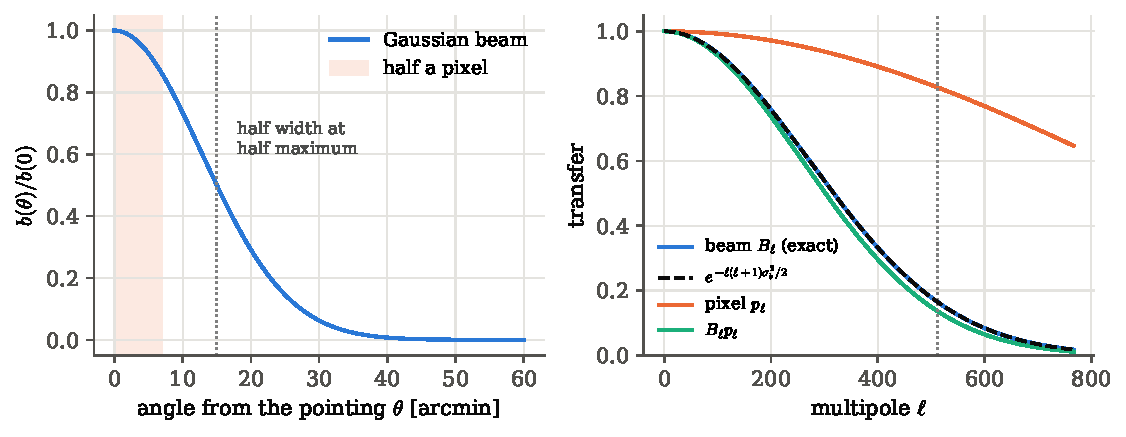
\includegraphics[width=12cm]{figures/ch08/beam_window.pdf}
\caption{Left: the Gaussian beam of the toy experiment as a function of the angle from the
pointing; the shaded band is half a pixel. Right: in harmonic space the beam becomes the
transfer function $B_\ell$. The exact Legendre transform (blue) and the formula
$e^{-\ell(\ell+1)\sigma_b^2/2}$ (dashed) are indistinguishable. The pixel window $p_\ell$
(orange) is a milder suppression; the product $B_\ell p_\ell$ (green) is what multiplies each
$\alm$. The dotted line marks the analysed range $\ell\le512$.}
\label{8a:fig:beam}
\end{figure}

\subsection{Pixel noise in harmonic space}
\label{8a:sec:noise}

The noise $n_p$ enters \eqref{8a:eq:obs-model} after the smoothing. To see what it does to
the spectrum we need its harmonic coefficients, which a map transform computes as a sum over
pixels, the quadrature version of $\int\dd\Omega$:
\begin{equation}
  n_{\ell m}=\Omega_{\rm pix}\sum_p n_p\,Y^*_{\ell m}(\hat{\bm n}_p).
  \label{8a:eq:nlm}
\end{equation}
Each $n_{\ell m}$ is a sum of independent Gaussian numbers, so it is Gaussian with mean zero.
Its covariance is
\begin{align}
  \langle n_{\ell m}\,n^*_{\ell'm'}\rangle
  &\eqby{1}\Omega_{\rm pix}^2\sum_{p,q}\langle n_p n_q\rangle\,Y^*_{\ell m}(\hat{\bm n}_p)\,Y_{\ell'm'}(\hat{\bm n}_q) \nonumber\\
  &\eqby{2}\Omega_{\rm pix}^2\sum_{p}\sigma_p^2\,Y^*_{\ell m}(\hat{\bm n}_p)\,Y_{\ell'm'}(\hat{\bm n}_p) \label{8a:eq:noise-cov-general}\\
  &\eqby{3}\sigma^2\,\Omega_{\rm pix}\sum_{p}\Omega_{\rm pix}\,Y^*_{\ell m}(\hat{\bm n}_p)\,Y_{\ell'm'}(\hat{\bm n}_p) \nonumber\\
  &\eqby{4}\sigma^2\,\Omega_{\rm pix}\,\delta_{\ell\ell'}\delta_{mm'} .
  \label{8a:eq:noise-cov}
\end{align}
\begin{explain}
  \item Insert \eqref{8a:eq:nlm} twice; the noise is real, $n_p^*=n_p$, and the average acts
        only on the noise.
  \item Different pixels are independent, $\langle n_pn_q\rangle=\sigma_p^2\delta_{pq}$.
  \item For uniform noise, $\sigma_p=\sigma$ in every pixel; split $\Omega_{\rm pix}^2$ into two factors.
  \item The remaining sum is the pixel approximation of $\int Y^*_{\ell m}Y_{\ell'm'}\dd\Omega=
        \delta_{\ell\ell'}\delta_{mm'}$, accurate for $\ell\lesssim2N_{\rm side}$ (\cref{ch:07}).
\end{explain}
Uniform, uncorrelated pixel noise is therefore \newterm{white} in harmonic space: every
$(\ell,m)$ gets an independent Gaussian of the same variance,
\begin{equation}
  N_\ell=\sigma^2\,\Omega_{\rm pix}\equiv\Delta_T^2 ,
  \label{8a:eq:nl}
\end{equation}
the \newterm{noise power spectrum} \srcref{Hivon}{§3.3}, \cite{Knox1995}. The cosmology notes
write it as $w^{-1}$, where $w\equiv(\Omega_{\rm pix}\sigma^2)^{-1}$ is the weight per solid
angle (see the cosmology notes).\footnote{In
\srcref{HobsonBMC}{(10.24)--(10.25)} the symbol $\sigma^2$ is the variance of the harmonic
noise coefficients, $\sigma^2_{\rm pix}\Omega_{\rm pix}$ in the notation here, not the
variance of a pixel; the two differ by a factor of order $10^{-5}$ for our pixels.} The square
root $\Delta_T=\sigma\sqrt{\Omega_{\rm pix}}$ is called the \newterm{map depth}, quoted in
$\mu$K\,arcmin \unpack{the noise of a pixel one arcminute on a side}. It is the natural label
of an experiment because it does not depend on how the map was pixelised: at a fixed total
observing time, a pixel half as large in area gets half the samples, so $\sigma^2$ doubles
and $\sigma^2\Omega_{\rm pix}$ stays the same.

\paragraph{Example: the toy experiment.}
Our experiment has depth $\Delta_T=\EightADepth\,\mu$K\,arcmin on $N_{\rm side}=\EightANside$
pixels of side $\EightAPixSide'$. The noise per pixel is
$\sigma=\Delta_T/\EightAPixSide'=\EightASigmaPix\,\mu$K, and
$N_\ell=(\EightADepth\times2.909\times10^{-4})^2\,\mu{\rm K}^2=\EightANell\,\mu$K$^2$, using
$1'=2.909\times10^{-4}$\,rad. On the map (\cref{8a:fig:maps}) the sky has an rms of
$\EightARmsSky\,\mu$K, the beam brings it down to $\EightARmsBeamed\,\mu$K, and the noise adds
$\EightARmsNoise\,\mu$K per pixel. By eye the noise is a faint grain on the large spots. In
harmonic space it dominates the beamed sky above $\ell\approx\EightALeq$ (\cref{8a:sec:noise-bias}).

\paragraph{Example: Knox's experiment.}
\textcite{Knox1995} considered a year of observation with $\sigma=22\,\mu$K in
$20'\times20'$ pixels. Its depth is $\Delta_T=22\times20=440\,\mu$K\,arcmin, or
$7.3\,\mu$K\,deg. He quotes the weight per solid angle $w=(7.5\,\mu{\rm K})^{-2}\,{\rm deg}^{-2}$,
which is the same number to the rounding in his $\sigma$. The same experiment pixelised into
$10'\times10'$ pixels would show $\sigma=44\,\mu$K per pixel and exactly the same $N_\ell$.

\begin{figure}[htbp]
\centering
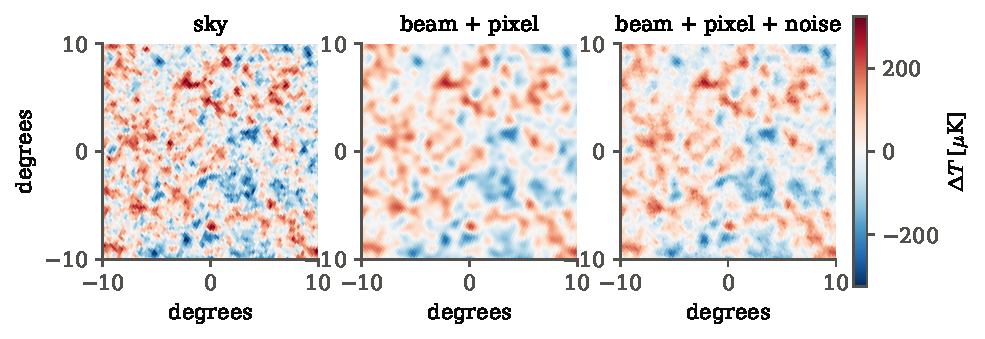
\includegraphics[width=12.5cm]{figures/ch08/observed_maps.pdf}
\caption{One simulated sky, $20^\circ$ on a side, before and after the instrument. Left: the
sky drawn from the fiducial $\Cell$. Middle: after the $30'$ beam and the $13.7'$ pixels; the
smallest spots are gone. Right: with $200\,\mu$K\,arcmin of white noise added, which shows up
as a fine grain. The colour scale is the same in all three panels.}
\label{8a:fig:maps}
\end{figure}

\begin{pitfall}[The beam acts on the sky, not on the noise]
In \eqref{8a:eq:obs-model} the noise is added after the smoothing, so the observed
coefficients are $d_{\ell m}=T_\ell\alm+n_{\ell m}$ and not $T_\ell(\alm+n_{\ell m})$.
The beam turns the sky down at high $\ell$ but leaves the noise at its full, flat level
\cite{Knox1995}. Dividing the observed coefficients by $T_\ell$ to undo the beam therefore
turns the noise up by $1/T_\ell$: the effective noise on the sky is $N_\ell/T_\ell^2$, which
grows like $e^{\ell(\ell+1)\sigma_b^2}$. A simulation that smooths the noise along with the sky
gets every error bar at high $\ell$ wrong.
\end{pitfall}

\paragraph{When the noise is not uniform.}
A scanning telescope does not visit every pixel equally often, and the noise variance of a
pixel falls as one over its number of hits \srcref{HobsonBMC}{(10.15)}. Then $\sigma_p$ changes
across the sky and step~(3) of \eqref{8a:eq:noise-cov} is no longer allowed. Line
\eqref{8a:eq:noise-cov-general} is still exact, and it says that the harmonic noise is no
longer diagonal: a pattern in $\sigma_p^2$ couples different $(\ell,m)$. One combination
survives untouched. Average the diagonal over the $2\ell+1$ values of $m$:
\begin{align}
  \bar N_\ell\equiv\frac{1}{2\ell+1}\sum_{m=-\ell}^{\ell}\langle|n_{\ell m}|^2\rangle
  &\eqby{1}\frac{\Omega_{\rm pix}^2}{2\ell+1}\sum_p\sigma_p^2\sum_{m}|Y_{\ell m}(\hat{\bm n}_p)|^2 \nonumber\\
  &\eqby{2}\frac{\Omega_{\rm pix}^2}{4\pi}\sum_p\sigma_p^2 \nonumber\\
  &\eqby{3}\Omega_{\rm pix}\,\langle\sigma^2\rangle .
  \label{8a:eq:nbar}
\end{align}
\begin{explain}
  \item Line \eqref{8a:eq:noise-cov-general} with $\ell'=\ell$, $m'=m$, summed over $m$.
  \item The addition theorem at coincident points, $\sum_m|Y_{\ell m}(\hat{\bm n})|^2=(2\ell+1)/4\pi$,
        the same for every direction.
  \item $N_{\rm pix}\Omega_{\rm pix}=4\pi$, and $\langle\sigma^2\rangle\equiv\sum_p\sigma_p^2/N_{\rm pix}$
        is the sky-averaged pixel variance.
\end{explain}
However the noise is distributed over the sky, the average noise power at every $\ell$ is
the pixel area times the mean pixel variance \cite[eq.~48]{Efstathiou2004}. This number fixes
the noise \emph{bias} of the next section. The noise \emph{scatter} depends on the full
pattern, and \cref{8a:sec:results} measures it.
\section{The noise bias and how to remove it}
\label{8a:sec:noise-bias}

Take the observed map of the toy experiment (\cref{8a:fig:maps}, right), transform it, and
average $|d_{\ell m}|^2$ over $m$ at $\ell=500$, exactly as \cref{ch:07} did for a perfect
sky. The answer comes out about four times larger than the beamed sky power $T_\ell^2\Cell$
at that multipole. Nothing went wrong in the transform. The noise in each $d_{\ell m}$
averages to zero, but its square does not: squaring a fluctuation turns it into power, and
power from the detector adds to power from the sky. Every spectrum computed from a noisy map
is biased upward, and the first task is to say by exactly how much.

Write the observed harmonic coefficients, using the transfer function $T_\ell=B_\ell p_\ell$ of
\eqref{8a:eq:transfer} and the harmonic noise $n_{\ell m}$ of \eqref{8a:eq:nlm}, as
$d_{\ell m}=T_\ell\alm+n_{\ell m}$, and define the \newterm{observed spectrum} as the same
average that gave $\Chat$ on a perfect sky:
\begin{equation}
  \widehat C^{\,\rm obs}_\ell\equiv\frac{1}{2\ell+1}\sum_{m=-\ell}^{\ell}|d_{\ell m}|^2 .
  \label{8a:eq:cobs}
\end{equation}
Its average over skies and noise realisations is
\begin{align}
  \bigl\langle\widehat C^{\,\rm obs}_\ell\bigr\rangle
  &\eqby{1}\frac{1}{2\ell+1}\sum_m\Bigl[T_\ell^2\langle|\alm|^2\rangle
     +T_\ell\langle\alm n^*_{\ell m}\rangle+T_\ell\langle\alm^*n_{\ell m}\rangle
     +\langle|n_{\ell m}|^2\rangle\Bigr] \nonumber\\
  &\eqby{2}\frac{1}{2\ell+1}\sum_m\Bigl[T_\ell^2\Cell+\langle|n_{\ell m}|^2\rangle\Bigr] \nonumber\\
  &\eqby{3}T_\ell^2\,\Cell+\bar N_\ell .
  \label{8a:eq:cobs-mean}
\end{align}
\begin{explain}
  \item Expand $|T_\ell\alm+n_{\ell m}|^2$; $T_\ell$ is real.
  \item The sky and the noise are independent and both have mean zero, so
        $\langle\alm n^*_{\ell m}\rangle=\langle\alm\rangle\langle n^*_{\ell m}\rangle=0$;
        statistical isotropy gives $\langle|\alm|^2\rangle=\Cell$ for every $m$ (\cref{ch:07}).
  \item The definition \eqref{8a:eq:nbar} of the mean noise power; for uniform noise
        $\bar N_\ell=N_\ell=\sigma^2\Omega_{\rm pix}$.
\end{explain}
The observed spectrum measures the beamed sky plus the noise. The excess $\bar N_\ell$ is the
\newterm{noise bias} \srcref{Hivon}{(15)}, \cite{Knox1995}. Because it is known, it can be
subtracted, and because $T_\ell$ is known, the beam can be divided out.

\begin{workdef}[debiased, deconvolved estimator]
For a full-sky map with transfer function $T_\ell$ and noise power $N_\ell$,
\begin{equation}
  \Chat=\frac{\widehat C^{\,\rm obs}_\ell-N_\ell}{T_\ell^2}
  \label{8a:eq:chat}
\end{equation}
\unpack{subtract the power the noise alone would give, then undo the suppression by the beam
and the pixel}. By \eqref{8a:eq:cobs-mean} it is unbiased, $\langle\Chat\rangle=\Cell$, for every
$\ell$.
\emph{Operationally:} compute \pyname{alm2cl(map2alm(d))}, subtract $N_\ell$ (from
\eqref{8a:eq:nl}, or from noise-only simulations when no formula exists), divide by
$B_\ell^2p_\ell^2$.
\end{workdef}

How large is the correction? The left panel of \cref{8a:fig:budget} plots the three spectra
of \eqref{8a:eq:cobs-mean} for the toy experiment. The beamed sky $T_\ell^2\Cell$ falls steeply
past $\ell\approx300$, while the noise $N_\ell$ is flat, and the two cross at
$\ell_{\rm eq}=\EightALeq$. Below $\ell_{\rm eq}$ the measurement is limited by the sky
itself; above it, by the detector.

\begin{figure}[htbp]
\centering
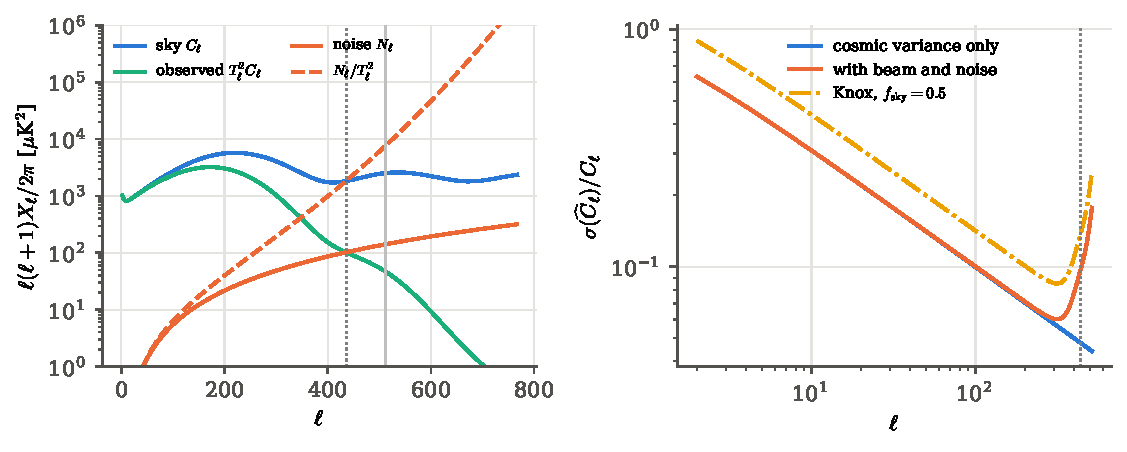
\includegraphics[width=12.5cm]{figures/ch08/budget.pdf}
\caption{The signal and noise budget of the toy experiment, plotted as
$\ell(\ell+1)X_\ell/2\pi$ for each spectrum $X_\ell$. Left: the sky spectrum (blue) is turned
down by the beam and pixel (green), while the white noise (orange, solid), flat in $N_\ell$,
rises only as $\ell^2$ in these units; the two cross at $\ell_{\rm eq}$ (dotted line). After dividing by $T_\ell^2$ the noise (orange, dashed) climbs
exponentially. The grey line marks the analysed range $\ell\le512$. Right: the fractional
error on $\Cell$ at a single multipole, from cosmic variance alone (blue), with the beam and
the noise (orange), and with Knox's sky-fraction factor for half the sky (yellow); the dotted line is again
$\ell_{\rm eq}$.}
\label{8a:fig:budget}
\end{figure}

\paragraph{Example: forgetting the subtraction.}
Without the subtraction the estimator $\widehat C^{\,\rm obs}_\ell/T_\ell^2$ is off by
$N_\ell/(T_\ell^2\Cell)$. For the toy experiment this is $\EightANoverSthree$ at $\ell=300$, a
$5\%$ excess, close to the cosmic-variance error of a single multipole there ($\EightAFracErrCVthree\%$). At
$\ell=512$ it is $\EightANoverSlmax$: the uncorrected spectrum is four times too high.

\subsection{Is this the best we can do?}
\label{8a:sec:ml}

The estimator \eqref{8a:eq:chat} was built by matching an average. The procedure of
\cref{ch:03} asks a different question: which value of $\Cell$ makes the data we observed most
probable? Say it in words first, in four moves.

The observed outcome is what the map gives us at one $\ell$: the coefficients $d_{\ell m}$. They
are complex, but only $2\ell+1$ real numbers are free, because the map is real and
$d_{\ell,-m}=(-1)^md^*_{\ell m}$ (\cref{ch:07}). To make these numbers all alike, rescale the
ones that come in pairs. The real $d_{\ell0}$ has variance $V_\ell$; for $m>0$ the variance
$V_\ell=\langle|d_{\ell m}|^2\rangle$ is shared equally between the real and imaginary parts, so
each of them has $V_\ell/2$. Define
\begin{align}
  u_1&\equiv d_{\ell0},\qquad
  u_{2m}\equiv\sqrt2\,\mathrm{Re}\,d_{\ell m},\qquad
  u_{2m+1}\equiv\sqrt2\,\mathrm{Im}\,d_{\ell m}\qquad(m=1,\dots,\ell),
  \label{8a:eq:u-def}\\
  \sum_{k=1}^{\nu}u_k^2
  &\eqby{1}d_{\ell0}^2+2\sum_{m=1}^{\ell}|d_{\ell m}|^2
   \eqby{2}\sum_{m=-\ell}^{\ell}|d_{\ell m}|^2
   \eqby{3}\nu\,\widehat C^{\,\rm obs}_\ell ,\qquad\nu=2\ell+1 .
  \nonumber
\end{align}
\begin{explain}
  \item $(\sqrt2\,\mathrm{Re}\,d)^2+(\sqrt2\,\mathrm{Im}\,d)^2=2|d|^2$.
  \item $|d_{\ell,-m}|=|d_{\ell m}|$, so the terms with $m<0$ repeat those with $m>0$.
  \item The definition \eqref{8a:eq:cobs} of the observed spectrum.
\end{explain}
Each $u_k$ now has the same variance $V_\ell$ and mean zero, and the $\nu$ of them are
independent. Every later count of ``$2\ell+1$ independent numbers'' at one $\ell$ refers to these
$u_k$.

The hypotheses are the possible values of $\Cell$. Under one of them, the model predicts mean
zero for every $u_k$; what turns that prediction into the numbers actually observed is a random
fluctuation, made of an independent sky part and an independent noise part. Variances of
independent Gaussians add, so under the hypothesis $\Cell$ the fluctuation is Gaussian with
variance $V_\ell=T_\ell^2\Cell+N_\ell$. The likelihood of $\Cell$ asks how plausible it is that a
fluctuation of that size produced exactly these $u_1,\dots,u_\nu$: too small a $\Cell$ makes the
observed values improbably large, too large a $\Cell$ makes them improbably small. Read as a
function of $\Cell$ with the data held fixed, that probability ranks the hypotheses; maximising
it, or combining it with a prior by Bayes' theorem, picks among them. Then
\begin{align}
  -2\ln\Like(\Cell)
  &\eqby{1}\sum_{k=1}^{\nu}\Bigl[\frac{u_k^2}{V_\ell}+\ln(2\pi V_\ell)\Bigr] \nonumber\\
  &\eqby{2}\nu\Bigl[\frac{\widehat C^{\,\rm obs}_\ell}{T_\ell^2\Cell+N_\ell}+\ln\bigl(T_\ell^2\Cell+N_\ell\bigr)\Bigr]+\text{const},
  \label{8a:eq:like-noise}\\
  \frac{\partial(-2\ln\Like)}{\partial\Cell}
  &\eqby{3}\nu\,T_\ell^2\Bigl[-\frac{\widehat C^{\,\rm obs}_\ell}{(T_\ell^2\Cell+N_\ell)^2}+\frac{1}{T_\ell^2\Cell+N_\ell}\Bigr]
   =0
   \;\Longrightarrow\;
   \hat C_\ell^{\rm ML}=\frac{\widehat C^{\,\rm obs}_\ell-N_\ell}{T_\ell^2}.
  \label{8a:eq:ml-noise}
\end{align}
\begin{explain}
  \item Each $u_k$ is $\Normal(0,V_\ell)$, with density $(2\pi V_\ell)^{-1/2}e^{-u_k^2/2V_\ell}$;
        independent densities multiply, so minus twice their logarithms add.
  \item $\sum_ku_k^2=\nu\widehat C^{\,\rm obs}_\ell$, and $V_\ell=T_\ell^2\Cell+N_\ell$; the
        $\ln2\pi$ terms do not depend on $\Cell$.
  \item Differentiate with the chain rule, $\partial V_\ell/\partial\Cell=T_\ell^2$; the bracket
        vanishes when $V_\ell=\widehat C^{\,\rm obs}_\ell$.
\end{explain}
The maximum-likelihood estimator is the debiased, deconvolved estimator
\srcref{HobsonBMC}{(10.24)--(10.25)}. On the full sky with uniform white noise, the cheap
estimator is not an approximation to the best one; it \emph{is} the best one, the
quadratic maximum-likelihood estimator of \cref{8a:sec:why-not-ml} with every matrix
diagonal. \Cref{8a:sec:variance} confirms that its variance reaches the Cram\'er--Rao bound.

One detail of \eqref{8a:eq:ml-noise} matters in practice. If the noise happens to fluctuate
low, $\widehat C^{\,\rm obs}_\ell<N_\ell$ and the estimate is negative, although $\Cell$ cannot
be. Restricting the maximum to $\Cell\ge0$ would replace those estimates by zero and bias the
average upward. We keep the unrestricted estimator, which is unbiased and can be negative,
and leave the constraint $\Cell\ge0$ to the likelihood in which $\Chat$ is later used
(\cref{ch:09}).

\subsection{When the noise level is not known exactly}
\label{8a:sec:noise-error}

The subtraction in \eqref{8a:eq:chat} needs $N_\ell$. For white, uniform noise
\eqref{8a:eq:nl} gives it. Real noise is coloured, varies across the sky, and is filtered
during map-making; then $N_\ell$ has no formula and is estimated by simulating noise-only
timestreams, making maps from them in the same way, and averaging their spectra,
$\langle\tilde N_\ell\rangle_{\rm MC}$ \srcref{Hivon}{§3.3}. Two questions follow: how much bias
does an error in $N_\ell$ cause, and how many noise simulations keep that error small?

\paragraph{Example: a 2\% error in the noise level.}
Subtract $(1+\varepsilon)N_\ell$ instead of $N_\ell$. By \eqref{8a:eq:cobs-mean} the average of
the estimator becomes $\Cell-\varepsilon N_\ell/T_\ell^2$, a fractional bias
\begin{equation}
  \frac{\langle\Chat\rangle-\Cell}{\Cell}=-\varepsilon\,\frac{N_\ell}{T_\ell^2\Cell} .
  \label{8a:eq:noise-error}
\end{equation}
At $\ell=512$, $N_\ell/(T_\ell^2\Cell)=\EightANoverSlmax$, so $\varepsilon=0.02$ gives $-6\%$. The
statistical error of one multipole there is $\EightAFracErrNlmax\%$ (\cref{8a:sec:variance}), and of
a bin of $25$ multipoles about $\EightAFracErrNlmax\%/\sqrt{25}\approx3.6\%$. A $2\%$ error in the
noise model produces a bias of almost two standard deviations per bin.

\begin{pitfall}[A small noise error is a large spectrum error at high $\ell$]
The bias \eqref{8a:eq:noise-error} is the noise error $\varepsilon$ times the noise-to-signal
ratio $N_\ell/(T_\ell^2\Cell)$, which grows like $e^{\ell(\ell+1)\sigma_b^2}$. However well the
noise is known, there is a multipole beyond which the auto-spectrum is dominated by the
uncertainty in the noise model rather than by the sky.
\end{pitfall}

\paragraph{Example: how many noise simulations?}
If $N_\ell$ is estimated as the average of the spectra of $N_n$ independent noise-only maps,
each of which scatters by $\sqrt{2/(2\ell+1)}\,N_\ell$ (the noise coefficients are Gaussian, so
their spectrum is a scaled $\chi^2$ like the sky's, \cref{ch:07}), the estimate scatters by
$\sqrt{2/(2\ell+1)}\,N_\ell/\sqrt{N_n}$. Compare it with the statistical error of
$\widehat C^{\,\rm obs}_\ell$, which is $\sqrt{2/(2\ell+1)}\,(T_\ell^2\Cell+N_\ell)$
(\cref{8a:sec:variance}):
\begin{equation}
  \frac{\text{error from the noise estimate}}{\text{statistical error}}
  =\frac{N_\ell}{T_\ell^2\Cell+N_\ell}\,\frac{1}{\sqrt{N_n}}\;\le\;\frac{1}{\sqrt{N_n}} .
  \label{8a:eq:nsim-noise}
\end{equation}
With $100$ noise simulations the extra error is at most $10\%$ of the statistical one. Errors
from independent sources add in quadrature, so the total error bar is at most
$\sqrt{1+0.1^2}=1.005$ times the statistical one: it grows by at most $0.5\%$. This is the number
Hivon et al.\ found for the Boomerang analysis \srcref{Hivon}{(42)}.

\subsection{Cross-spectra: no noise bias at all}
\label{8a:sec:cross}

There is a way to avoid the noise model entirely. Split the data in two: the first and second
halves of the mission, or two sets of detectors. Each half sees the same sky through the same
beam, $d^{(i)}_{\ell m}=T_\ell\alm+n^{(i)}_{\ell m}$ for $i=1,2$, but the two noise realisations
are independent. Instead of squaring one map, multiply the two:
\begin{equation}
  \widehat C^{\,12}_\ell\equiv\frac{1}{2\ell+1}\sum_m{\rm Re}\bigl(d^{(1)}_{\ell m}d^{(2)*}_{\ell m}\bigr),
  \qquad
  \bigl\langle\widehat C^{\,12}_\ell\bigr\rangle=T_\ell^2\Cell+\bigl\langle{\rm Re}\,n^{(1)}_{\ell m}n^{(2)*}_{\ell m}\bigr\rangle=T_\ell^2\Cell .
  \label{8a:eq:cross}
\end{equation}
The cross terms between sky and noise vanish as in \eqref{8a:eq:cobs-mean}, and the
noise--noise term vanishes because the two noises are independent. The
\newterm{cross-spectrum} has no noise bias, and it needs no noise model
\cite{HamimecheLewis2008}. The Planck high-$\ell$ likelihood is built from cross-spectra
between half-mission maps for exactly this reason \cite{Planck2018V}
(\cref{8a:fig:cross-diagram}).

\begin{figure}[htbp]
\centering
\begin{tikzpicture}[
  bx/.style={draw=accent,thick,rounded corners=2pt,fill=ideabg,font=\small,
             minimum height=9mm,align=center,text width=30mm},
  ok/.style={draw=tangentgreen!80!black,thick,rounded corners=2pt,fill=white,font=\small,
             minimum height=8mm,align=center,text width=26mm},
  no/.style={draw=bdryred!80!black,thick,rounded corners=2pt,fill=white,font=\small,
             minimum height=8mm,align=center,text width=26mm},
  flow/.style={->,thick,accent}]
  \node[bx] (a) at (0,1.2)  {half 1: $T\,a+n^{(1)}$};
  \node[bx] (b) at (0,-1.2) {half 2: $T\,a+n^{(2)}$};
  \node[draw=accent,thick,circle,inner sep=1pt,font=\small] (x) at (3.2,0) {$\times$};
  \node[ok] (ss) at (7.0,1.5)  {$T^2\langle|a|^2\rangle=T^2\Cell$};
  \node[ok] (sn) at (7.0,0)    {sky $\times$ noise: $0$};
  \node[ok] (nn) at (7.0,-1.5) {$\langle n^{(1)}n^{(2)*}\rangle=0$};
  \node[no] (au) at (11.0,-1.5) {auto: $\langle|n|^2\rangle=N_\ell$};
  \draw[flow] (a.east) -- (x); \draw[flow] (b.east) -- (x);
  \draw[flow] (x) -- (ss.west); \draw[flow] (x) -- (sn.west); \draw[flow] (x) -- (nn.west);
  \draw[densely dashed,bdryred!70!black,thick] (nn.east) -- (au.west);
\end{tikzpicture}
\caption{Why the cross-spectrum has no noise bias. Multiplying two maps of the same sky with
independent noise leaves three kinds of terms on average: the sky power survives, sky times
noise averages to zero, and noise times the \emph{other} noise averages to zero. In the
auto-spectrum (red) the last term is a noise times itself, whose average is the noise power.}
\label{8a:fig:cross-diagram}
\end{figure}

The price is paid in scatter. Each half has twice the noise variance of the full map,
$N^{(1)}_\ell=N^{(2)}_\ell=2N_\ell$, because it has half the observing time. To find the variance
of \eqref{8a:eq:cross}, write it, as for the likelihood above, as a sum over the $\nu=2\ell+1$
real degrees of freedom, $\nu\widehat C^{\,12}_\ell=\sum_k u_kv_k$, where $u_k$ and $v_k$ are the
corresponding real components of the two maps. The pairs are independent for different $k$;
within a pair $u$ and $v$ are zero-mean Gaussians with variances $S+2N$ each (writing $S=T_\ell^2\Cell$,
$N=N_\ell$) and covariance $\langle uv\rangle=S$, since only the sky is shared. Then
\begin{align}
  \Var(uv)
  &\eqby{1}\langle u^2v^2\rangle-\langle uv\rangle^2 \nonumber\\
  &\eqby{2}\langle u^2\rangle\langle v^2\rangle+2\langle uv\rangle^2-\langle uv\rangle^2 \nonumber\\
  &\eqby{3}(S+2N)^2+S^2 ,
  \label{8a:eq:var-uv}\\
  \Var\bigl(\widehat C^{\,12}_\ell\bigr)
  &\eqby{4}\frac{(S+2N)^2+S^2}{2\ell+1}
  \quad\text{versus}\quad
  \Var\bigl(\widehat C^{\,\rm obs}_\ell\bigr)=\frac{2(S+N)^2}{2\ell+1}.
  \label{8a:eq:var-cross}
\end{align}
\begin{explain}
  \item Definition of the variance.
  \item Isserlis' theorem for zero-mean Gaussians (\cref{ch:07}): $\langle uuvv\rangle$ is the sum
        over the three ways of pairing the four factors.
  \item Insert the variances and the covariance.
  \item The $\nu$ terms are independent, so their variances add, and dividing the sum by $\nu$
        divides the variance by $\nu^2$. The auto-spectrum line is the case $u=v$ with variance
        $S+N$, derived in \cref{8a:sec:variance}.
\end{explain}
When the sky dominates ($N\ll S$) both variances are $2S^2/\nu$: nothing is lost. When the
noise dominates ($S\ll N$) the cross-spectrum variance is $4N^2/\nu$ against $2N^2/\nu$, so its
error bar is $\sqrt2$ times larger. At $\ell=512$ the predicted ratio of error bars is
$\EightACrossRatioLmax$; the simulations of \cref{8a:sec:results} find $\EightACrossRatioMCLast$.
The cross-spectrum trades a little precision for immunity to the noise model, a trade that
real analyses usually accept.
\section{How much the estimate scatters}
\label{8a:sec:variance}

The debiased, deconvolved estimator $\Chat=(\widehat C^{\,\rm obs}_\ell-N_\ell)/T_\ell^2$ of
\eqref{8a:eq:chat} centres on the true spectrum. Here $\widehat C^{\,\rm obs}_\ell$ is the
average of $|d_{\ell m}|^2$ over $m$ on the observed map, $N_\ell$ the noise power and
$T_\ell=B_\ell p_\ell$ the beam times the pixel window (\cref{8a:sec:model}). Centring on the
truth is a statement about the average over many skies. We have one sky, and on it a single
estimate at $\ell=512$ typically lands about a fifth away from $\Cell$. On a perfect sky the
same estimate would land only about $4\%$ away. Something in the observation has made the
scatter four times larger, and we want to know what, by how much at every $\ell$, and whether
any other estimator could do better.

Said in words, there are four questions. How wide is the spread of $\Chat$ over skies and
noise realisations? How much of it comes from the sky and how much from the detector? Is it
the smallest spread any estimator could achieve with these data? And what is the full shape
of the distribution, not just its width?

\paragraph{The width.}
The answer comes from the same bookkeeping that gave the likelihood in \cref{8a:sec:ml}. At
one $\ell$ the observed map supplies $\nu=2\ell+1$ real numbers $u_1,\dots,u_\nu$, the
coefficients $d_{\ell m}$ rescaled so that all have the same variance, \eqref{8a:eq:u-def}. Each is
a sky part plus an independent noise part, so each is a zero-mean Gaussian with variance
$V_\ell=T_\ell^2\Cell+N_\ell$, they are independent of one another, and
$\sum_ku_k^2=\nu\,\widehat C^{\,\rm obs}_\ell$. A sum of $\nu$ squared
independent standard Gaussians is a $\chi^2_\nu$ variable, whose variance is $2\nu$
(\cref{ch:07}). Then
\begin{align}
  \Var\bigl(\Chat\bigr)
  &\eqby{1}\frac{1}{T_\ell^4}\Var\bigl(\widehat C^{\,\rm obs}_\ell\bigr)
   \eqby{2}\frac{1}{T_\ell^4}\,\frac{V_\ell^2}{\nu^2}\,\Var\Bigl(\sum_{k=1}^{\nu}\frac{u_k^2}{V_\ell}\Bigr)
   \nonumber\\
  &\eqby{3}\frac{1}{T_\ell^4}\,\frac{V_\ell^2}{\nu^2}\,2\nu
   \eqby{4}\frac{2}{2\ell+1}\Bigl(\Cell+\frac{N_\ell}{T_\ell^2}\Bigr)^2 .
  \label{8a:eq:var}
\end{align}
\begin{explain}
  \item $N_\ell$ and $T_\ell$ are fixed numbers: subtracting a constant does not change a
        variance, and dividing by $T_\ell^2$ divides it by $T_\ell^4$.
  \item $\widehat C^{\,\rm obs}_\ell=\frac1\nu\sum_ku_k^2=\frac{V_\ell}{\nu}\sum_k(u_k^2/V_\ell)$,
        and a constant factor comes out of a variance squared.
  \item Each $u_k/\sqrt{V_\ell}$ is a standard Gaussian, so the sum is $\chi^2_\nu$, with variance $2\nu$.
  \item $V_\ell/T_\ell^2=\Cell+N_\ell/T_\ell^2$ and $\nu=2\ell+1$.
\end{explain}

\begin{keyidea}[The error bar of a full-sky, beamed, noisy spectrum]
\[
  \sigma\bigl(\Chat\bigr)=\sqrt{\frac{2}{2\ell+1}}\,\Bigl(\Cell+\frac{N_\ell}{T_\ell^2}\Bigr).
\]
The sky and the noise enter added, inside the bracket, and the noise enters as it looks
\emph{after} the beam has been divided out, $N_\ell/T_\ell^2$.
\end{keyidea}

This is the formula of \textcite[eq.~4]{Knox1995}, written there with the weight per solid
angle $w^{-1}=N_\ell$ and a Gaussian beam, $T_\ell^2\to e^{-\ell^2\sigma_b^2}$. The cosmology
notes reach it as the inverse square root of the Fisher information of $\Cell$, with the
window $W_\ell=B_\ell^2$ (see the cosmology notes). With no noise it is the cosmic variance of
\cref{ch:07}. Knox also explained the factor $2/(2\ell+1)$ in words: the error on a variance
measured from $n$ Gaussian samples is $2\sigma^4/n$, however precisely each sample is
measured, and the sky offers $2\ell+1$ samples at each $\ell$ \srcref{Knox1995}{p.~8}.

\paragraph{Where the variance comes from.}
Squaring the bracket in \eqref{8a:eq:var} splits the variance into three terms,
\begin{equation}
  \Var\bigl(\Chat\bigr)=\frac{1}{2\ell+1}\Bigl[\,\underbrace{2\Cell^2}_{\text{sky}}
   +\underbrace{4\,\Cell\,\frac{N_\ell}{T_\ell^2}}_{\text{sky}\times\text{noise}}
   +\underbrace{2\Bigl(\frac{N_\ell}{T_\ell^2}\Bigr)^2}_{\text{noise}}\,\Bigr].
  \label{8a:eq:var-terms}
\end{equation}
The first is the cosmic variance, which no instrument can remove. The last is the scatter of
the noise power itself, which would be there with no sky at all. The middle one is easy to
overlook. Each observed coefficient is a sum of a sky part and a noise part, so
$|d_{\ell m}|^2$ contains the product of the two. That product averages to zero, which is
why it did not appear in the bias \eqref{8a:eq:cobs-mean}, but it fluctuates, and its
fluctuation is the cross term.

\paragraph{Example: when does the noise supply half the variance?}
Write $r=N_\ell/(T_\ell^2\Cell)$ for the noise-to-signal ratio on the sky. The two terms of
\eqref{8a:eq:var-terms} that involve the noise make up half of the total when
\begin{align}
  4r+2r^2=\tfrac12\bigl(2+4r+2r^2\bigr)
  \;\eqby{1}\;r^2+2r-1=0
  \;\eqby{2}\;r=\sqrt2-1\approx0.41 .
  \nonumber
\end{align}
\begin{explain}
  \item Divide \eqref{8a:eq:var-terms} by $\Cell^2/(2\ell+1)$, multiply out and collect terms.
  \item The positive root of the quadratic.
\end{explain}
The noise already supplies half the variance when its power on the sky is $41\%$ of the
signal, well before the two powers are equal. At equality, $r=1$, the noise terms are
$6/8=75\%$ of the variance. In the toy experiment of \cref{8a:sec:noise} (a $30'$ beam and
$200\,\mu$K\,arcmin of white noise on $N_{\rm side}=256$ pixels) the two powers cross at
$\ell_{\rm eq}=\EightALeq$, but the noise supplies half the variance from
$\ell=\EightALHalfNoiseVar$ onward.

\paragraph{Example: the error bar at three multipoles.}
At $\ell=300$ the cosmic variance alone gives a fractional error
$\sqrt{2/601}=\EightAFracErrCVthree\%$, and the noise, with $r=\EightANoverSthree$, raises it
to $\EightAFracErrNthree\%$. At $\ell=512$ the cosmic variance gives
$\sqrt{2/1025}=\EightAFracErrCVlmax\%$, but $r=\EightANoverSlmax$ multiplies it by $1+r$, to
$\EightAFracErrNlmax\%$: the factor of four of the opening paragraph. At $\ell=700$, beyond
the analysed band, $r=\EightANoverSseven$ and the fractional error is $\EightAFracErrNseven$,
nearly a thousand per cent. The right panel of \cref{8a:fig:budget} plots the whole curve.

\paragraph{The smallest possible width.}
Is there a better estimator? The Cram\'er--Rao bound of \cref{ch:03} says no unbiased
estimator can have a variance below one over the Fisher information,
$I(\Cell)=\bigl\langle\partial^2(-\ln\Like)/\partial\Cell^2\bigr\rangle$. With
$-\ln\Like=\frac\nu2\bigl[\widehat C^{\,\rm obs}_\ell/V_\ell+\ln V_\ell\bigr]+\text{const}$ from
\eqref{8a:eq:like-noise}, and $\partial V_\ell/\partial\Cell=T_\ell^2$,
\begin{align}
  \frac{\partial(-\ln\Like)}{\partial\Cell}
  &\eqby{1}\frac{\nu}{2}\,T_\ell^2\Bigl[-\frac{\widehat C^{\,\rm obs}_\ell}{V_\ell^2}+\frac{1}{V_\ell}\Bigr],
  \nonumber\\
  I(\Cell)
  &\eqby{2}\frac{\nu}{2}\,T_\ell^4\Bigl[\frac{2\langle\widehat C^{\,\rm obs}_\ell\rangle}{V_\ell^3}-\frac{1}{V_\ell^2}\Bigr]
   \eqby{3}\frac{\nu\,T_\ell^4}{2V_\ell^2}
   \eqby{4}\frac{2\ell+1}{2\,(\Cell+N_\ell/T_\ell^2)^2} .
  \label{8a:eq:fisher-cl}
\end{align}
\begin{explain}
  \item Chain rule on both terms.
  \item Differentiate once more (again $\partial V_\ell/\partial\Cell=T_\ell^2$) and average over the data.
  \item $\langle\widehat C^{\,\rm obs}_\ell\rangle=V_\ell$ by \eqref{8a:eq:cobs-mean}, so the bracket is $1/V_\ell^2$.
  \item $V_\ell/T_\ell^2=\Cell+N_\ell/T_\ell^2$.
\end{explain}
One over \eqref{8a:eq:fisher-cl} is exactly \eqref{8a:eq:var}. The debiased estimator reaches
the bound: on the full sky with uniform white noise it extracts every bit of information
about $\Cell$ that the map contains. Whatever an estimator on a masked sky loses is measured
against this number.

\subsection{The shape of the distribution}
\label{8a:sec:shape}

The width is not the whole story; the likelihood of \cref{ch:09} needs the full distribution.
It follows from the same bookkeeping that gave the width \eqref{8a:eq:var} and the bound
\eqref{8a:eq:fisher-cl}. There, the $\nu=2\ell+1$ real numbers $u_k$ at one $\ell$ were independent
Gaussians of variance $V_\ell=T_\ell^2\Cell+N_\ell$, so
$X\equiv\sum_ku_k^2/V_\ell=\nu\,\widehat C^{\,\rm obs}_\ell/V_\ell$ is a $\chi^2_\nu$ variable. Solve
for $\widehat C^{\,\rm obs}_\ell=V_\ell X/\nu$ and insert it in the estimator \eqref{8a:eq:chat},
with the noise-to-signal ratio $r_\ell\equiv N_\ell/(T_\ell^2\Cell)$ of \cref{8a:sec:variance}:
\begin{align}
  \frac{\Chat}{\Cell}
  &\eqby{1}\frac{\widehat C^{\,\rm obs}_\ell-N_\ell}{T_\ell^2\Cell}
   \eqby{2}\frac{V_\ell}{\nu\,T_\ell^2\Cell}\,X-\frac{N_\ell}{T_\ell^2\Cell}
   \nonumber\\
  &\eqby{3}A_\ell\,X-r_\ell,
  \qquad X\sim\chi^2_{2\ell+1},
  \qquad A_\ell=\frac{1+r_\ell}{2\ell+1}.
  \label{8a:eq:shifted-chi2}
\end{align}
\begin{explain}
  \item The definition \eqref{8a:eq:chat}, divided by $\Cell$.
  \item $\widehat C^{\,\rm obs}_\ell=V_\ell X/\nu$.
  \item $V_\ell/(T_\ell^2\Cell)=1+N_\ell/(T_\ell^2\Cell)=1+r_\ell$, and $\nu=2\ell+1$.
\end{explain}
The debiased estimator is a scaled and shifted $\chi^2$. Its variance closes the loop with the
previous subsection: $\Var(\Chat/\Cell)=A_\ell^2\Var(X)=A_\ell^2\,2\nu=2(1+r_\ell)^2/(2\ell+1)$, so
$\Var(\Chat)=2(\Cell+N_\ell/T_\ell^2)^2/(2\ell+1)$, which is \eqref{8a:eq:var} and one over the
Fisher information \eqref{8a:eq:fisher-cl}. The distribution \eqref{8a:eq:shifted-chi2} is the
full shape whose width sits exactly on the Cram\'er--Rao bound. The appendix of
\textcite{Knox1995} derives the same density (his eqs.~31--33). Two features follow at once.
At low $\ell$, $\nu$ is small and the $\chi^2$ is visibly skewed. How skewed follows from its
cumulants. A $\chi^2_\nu$ is a sum of $\nu$ independent squared standard Gaussians, cumulants of
independent terms add, and each square contributes $\kappa_k=2^{k-1}(k-1)!$; so
$\kappa_k=2^{k-1}(k-1)!\,\nu$ for the sum, as derived in \eqref{7b:eq:chi2-cumulants}. The
skewness is the third cumulant over the variance to the power $3/2$,
\begin{equation}
  \frac{\kappa_3}{\kappa_2^{3/2}}=\frac{8\nu}{(2\nu)^{3/2}}=\sqrt{\frac8\nu},
  \qquad\text{and likewise the excess kurtosis is}\qquad
  \frac{\kappa_4}{\kappa_2^2}=\frac{48\nu}{(2\nu)^2}=\frac{12}{\nu}.
  \label{8a:eq:chi2-shape}
\end{equation}
Scaling and shifting the variable, as in \eqref{8a:eq:shifted-chi2}, changes neither ratio. The
skewness is $\EightASkewThreeTh$ at $\ell=3$. And the shift $-r_\ell$ moves part of
the distribution below zero. The estimate is negative whenever the observed power happens to
fall below the noise power, $X<\nu\,r_\ell/(1+r_\ell)$, which becomes likely once $r_\ell$ is
large.

\paragraph{Example: how often is the estimate negative?}
At $\ell_{\rm eq}=\EightALeq$, where $r_\ell=1$, a negative estimate needs $X<\nu/2$, a
$\chi^2_{873}$ variable more than ten standard deviations below its mean: the probability
is $\EightAPnegLeq$. At $\ell=700$, $r_\ell=\EightANoverSseven$ and the threshold
$\nu r_\ell/(1+r_\ell)$ sits within a fraction of a standard deviation of the mean $\nu$. The
probability of a negative estimate is then $\EightAPnegSeven\%$ (\cref{8a:fig:debiased-pdf},
right). A negative $\Chat$ there is not a sign of a bug. The measurement simply contains
almost no signal, and the unbiased estimator has to straddle zero.

\begin{figure}[htbp]
\centering
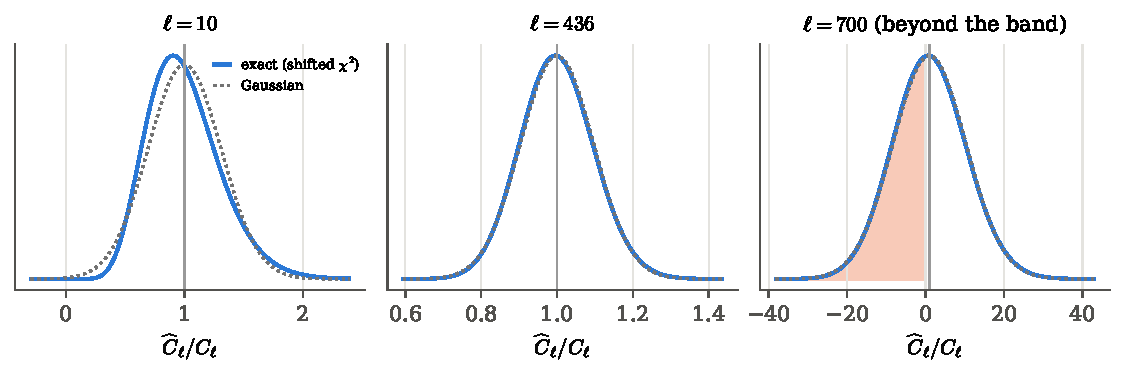
\includegraphics[width=12.5cm]{figures/ch08/debiased_pdf.pdf}
\caption{The exact distribution of $\Chat/\Cell$ for the toy experiment at three multipoles
(blue), with the Gaussian of the same mean and width (dotted). At $\ell=10$ the $\chi^2$ is
skewed, with its peak below the mean. At $\ell=\EightALeq$ it is close to Gaussian and safely
positive. At $\ell=700$, outside the analysed band, it is a broad Gaussian centred on $1$,
almost half of which (orange) lies below zero.}
\label{8a:fig:debiased-pdf}
\end{figure}

\subsection{Knox's formula on part of the sky}
\label{8a:sec:knox}

Knox's formula was derived for a complete sky. Every real temperature analysis cuts away the
Galaxy, and every ground or balloon experiment sees a patch. The approximation used
everywhere for that case divides the variance by the observed sky fraction $\fsky$ and, when
$\Delta\ell$ neighbouring multipoles are averaged into one bin, by $\Delta\ell$ as well:
\begin{equation}
  \sigma\bigl(\widehat C_b\bigr)\approx\sqrt{\frac{2}{(2\ell+1)\,\Delta\ell\,\fsky}}\,
  \Bigl(\Cell+\frac{N_\ell}{T_\ell^2}\Bigr)
  \label{8a:eq:knox-fsky}
\end{equation}
\srcref{Hivon}{(16)--(17)}, \cite[eq.~33]{Efstathiou2004} (see also the cosmology notes). Each of
its two new factors comes from one move applied to the full-sky error \eqref{8a:eq:var}.
\begin{itemize}
  \item \emph{The bin.} The binned estimate $\widehat C_b$ is the plain average of the
        $\Delta\ell$ values $\Chat$ in the bin. On the full sky they are independent, so their
        variances add, and the $1/\Delta\ell$ of the average comes out squared:
        $\Var(\widehat C_b)=\Delta\ell^{-2}\sum_{\ell\in b}\Var(\Chat)$. If the spectrum changes
        little across the bin, the $\Delta\ell$ terms are all about equal, the sum is $\Delta\ell$
        times one of them, and $2/(2\ell+1)$ becomes $2/[(2\ell+1)\Delta\ell]$.
  \item \emph{The sky fraction.} The factor $2/(2\ell+1)$ is $2/\nu$, with $\nu$ the number of
        independent modes. A patch covering a fraction $\fsky$ of the sky is taken to carry that
        fraction of the modes, $\nu\to\nu\,\fsky$, which divides the variance by $\fsky$.
\end{itemize}
The same two moves are written out as labelled chains where we reproduce the papers that use the
formula: \eqref{8a:eq:hivon16} for the bin, \eqref{8a:eq:knox5-fsky} for the sky fraction.
\textcite{Hivon2002} add a factor $w_2^2/w_4$ to $\fsky$ for a weighted mask, where
$w_i$ is the sky average of the $i$-th power of the mask over the observed region
\srcref{Hivon}{(17)}.

The plain claim is: \emph{observing half the sky doubles the variance}. The everyday question
behind it is, how many independent numbers does a patch of sky provide at multipole $\ell$?
On the full sky the answer is $2\ell+1$, one per $m$, and they are independent, which is why
the error is $\sqrt{2/(2\ell+1)}$. The formula assumes that a fraction $\fsky$ of the sky
provides the same fraction of independent numbers, $(2\ell+1)\fsky$, and that each still
belongs to a single $\ell$. That is the hidden assumption: the modes on the patch are taken to
be as clean as on the full sky, only fewer.

It cannot be literally true, and three short moves show why. First, the observed map is the
sky times the mask, $s(\hat{\bm n})M(\hat{\bm n})$, with $M=1$ inside the patch and $0$ outside.
Second, expand both factors in spherical harmonics. A product $Y_{\ell'm'}Y_{LM}$ is again a sum
of spherical harmonics, but of every degree from $|\ell'-L|$ to $\ell'+L$ (the rule for adding
angular momenta), so a coefficient of degree $\ell$ of the cut map collects sky coefficients
$a_{\ell'm'}$ from every $\ell'$ that differs from $\ell$ by a degree $L$ present in the mask. A
patch of angular size $\theta_{\rm p}$ has its harmonic content concentrated at
$L\lesssim\pi/\theta_{\rm p}$, so each $\ell$ of the cut map mixes the sky over a width
$\Delta\ell_c\sim\pi/\theta_{\rm p}$ around it. Third, two neighbouring multipoles of the cut map
then share sky modes and are correlated; the power of one $\ell$ is spread over its neighbours.
This is called \newterm{mode coupling} \srcref{Hivon}{(14)}. The modes on a patch are shared between
multipoles, so the counting is right only on average over a bin wider than $\Delta\ell_c$, which
is why the formula comes with a bin width $\Delta\ell$. The coupling is computed exactly for the
masked sky in \cref{8b:sec:kernel}.

\paragraph{Example: the counting fails where there is less than one mode.}
Hivon et al.'s test region covers $\fsky=1.82\%$ of the sky \srcref{Hivon}{§4.1}. For the
quadrupole, $(2\ell+1)\fsky=0.09$: the formula claims a tenth of one mode and an error bar
$\sqrt{2/0.09}\approx4.7$ times the signal. A patch $40^\circ\times24^\circ$ cannot contain a
single wavelength of the quadrupole, so it cannot tell a quadrupole from a dipole or from an
$\ell=3$ pattern. The question ``how well is $C_2$ measured?'' has no separate answer there, and
no counting rule can supply one. \Textcite{Efstathiou2004} shows by comparing with the exact
maximum-likelihood Fisher matrix that the $\fsky$ formula fails at low $\ell$ even for large
sky fractions.

\paragraph{Example: the counting works where there are many.}
In the same region, take a bin of $\Delta\ell=50$ around $\ell=200$. The number of modes is
$(2\cdot200+1)\times50\times0.0182=365$, and \eqref{8a:eq:knox-fsky} gives a fractional error
of $\sqrt{2/365}=7.4\%$ on the signal-dominated bin. With the cosine-apodised weighting of
their Table~1, $w_2^2/w_4=0.514$, the count drops to $188$ and the error rises to $10.3\%$.
Hivon et al.\ found that their simulated error bars match this rule of thumb almost exactly
\srcref{Hivon}{(36), §4.2}.

\begin{figure}[htbp]
\centering
\begin{tikzpicture}[x=0.95cm,y=0.3cm]
  \foreach \l in {0,...,9}{
    \foreach \m in {-\l,...,\l}{
      \fill[formblue!70] (\l,\m) circle (1.6pt);
    }
  }
  \fill[fibreorange!25,rounded corners=2pt] (5.6,-8.8) rectangle (8.4,8.8);
  \foreach \l in {6,7,8}{
    \foreach \m in {-\l,...,\l}{
      \fill[fibreorange!90!black] (\l,\m) circle (1.8pt);
    }
  }
  \draw[->,thick,softgray!60!black] (-0.6,0) -- (10.2,0) node[right,font=\small] {$\ell$};
  \draw[->,thick,softgray!60!black] (-0.6,-10.2) -- (-0.6,10.4) node[above,font=\small] {$m$};
  \foreach \l in {0,3,6,9}{\node[font=\scriptsize,below] at (\l,-10.0) {$\l$};}
  \node[font=\scriptsize,align=left,anchor=west] at (10.3,6.0)
       {column $\ell$:\\ $2\ell+1$ independent modes};
  \node[font=\scriptsize,align=left,anchor=west,fibreorange!80!black] at (10.3,-5.5)
       {bin of $\Delta\ell=3$:\\ $\sum(2\ell+1)=45$ modes;\\ a sky fraction $\fsky$\\ keeps about $45\,\fsky$};
\end{tikzpicture}
\caption{Counting modes. Each dot is one independent number on the full sky, one per
$(\ell,m)$; column $\ell$ has $2\ell+1$ of them. A bin of $\Delta\ell$ multipoles (orange)
contains about $(2\ell+1)\Delta\ell$. The $\fsky$ rule assumes that a patch of sky keeps the
fraction $\fsky$ of these dots, each still in its own column. A mask actually smears every dot
over neighbouring columns, so the rule can hold only for bins wider than the smearing.}
\label{8a:fig:modes}
\end{figure}

\begin{pitfall}[The $\fsky$ formula is a count, not a theorem]
Equation \eqref{8a:eq:knox-fsky} counts modes. It is reliable only for bins that contain many
modes and are wider than the coupling a mask induces between multipoles. At low $\ell$, for
small patches, and for the correlations between neighbouring bins, it says nothing; there the
covariance must come from simulations or from the exact mode-coupling matrix of the masked
sky \srcref{Hivon}{§3.1}.
\end{pitfall}

\subsection{Signal-to-noise, per multipole and in total}
\label{8a:sec:snr}

How well does each multipole measure the spectrum? The natural number is the
\newterm{signal-to-noise per multipole}, the spectrum divided by its own error bar, from
\eqref{8a:eq:var}:
\begin{equation}
  \SNR_\ell\equiv\frac{\Cell}{\sigma(\Chat)}=\sqrt{\frac{2\ell+1}{2}}\;\frac{\Cell}{\Cell+N_\ell/T_\ell^2}
  =\sqrt{\frac{2\ell+1}{2}}\;\frac{1}{1+r_\ell}.
  \label{8a:eq:snr-ell}
\end{equation}
With no noise it grows as $\sqrt{\ell}$, because higher multipoles have more modes. The noise
cuts it by the factor $1/(1+r_\ell)$, which falls exponentially once the beam has turned the
sky down. Between these two behaviours there is a best multipole. For the toy experiment it is
$\ell=\EightASnrPeakEll$, with $\SNR_\ell=\EightASnrPeak$; at $\ell_{\rm eq}$ the value has fallen
to $\EightASnrEq$ (\cref{8a:fig:snr}, left).

A second question is how well all multipoles together measure the spectrum. Since one
number per $\ell$ is too much to summarise, ask about the simplest possible change of the
spectrum: an overall amplitude, $\Cell=A\,C^{\rm fid}_\ell$ with $A=1$ for the true sky. Each
multipole gives an independent unbiased estimate of $A$, namely $\Chat/C^{\rm fid}_\ell$, with
variance $1/\SNR_\ell^2$. Independent estimates of one number are best combined with weights
proportional to their inverse variances (\cref{ch:03}):
\begin{align}
  \hat A&=\frac{\sum_\ell\SNR_\ell^2\,\Chat/C^{\rm fid}_\ell}{\sum_\ell\SNR_\ell^2},
  \nonumber\\
  \Var(\hat A)
  &\eqby{1}\frac{\sum_\ell\SNR_\ell^4\,\Var(\Chat/C^{\rm fid}_\ell)}{\bigl(\sum_\ell\SNR_\ell^2\bigr)^2}
   \eqby{2}\frac{\sum_\ell\SNR_\ell^2}{\bigl(\sum_\ell\SNR_\ell^2\bigr)^2}
   =\frac{1}{\sum_\ell\SNR_\ell^2} .
  \label{8a:eq:amp}
\end{align}
\begin{explain}
  \item The terms are independent (different $\ell$ on the full sky), so variances add, each
        multiplied by the square of its weight.
  \item $\Var(\Chat/C^{\rm fid}_\ell)=1/\SNR_\ell^2$ by the definition \eqref{8a:eq:snr-ell}.
\end{explain}

\begin{workdef}[cumulative signal-to-noise]
\[
  \SNR(\le\ell_{\max})\equiv\Bigl[\sum_{\ell=2}^{\ell_{\max}}\SNR_\ell^2\Bigr]^{1/2}
  =\Bigl[\sum_{\ell=2}^{\ell_{\max}}\frac{2\ell+1}{2}\,\frac{1}{(1+r_\ell)^2}\Bigr]^{1/2}
\]
\unpack{the number of standard deviations by which the spectrum up to $\ell_{\max}$ is
detected, if only its overall amplitude is fitted}. \emph{Operationally:} one over the error
of the amplitude $\hat A$ of \eqref{8a:eq:amp}.
\end{workdef}

The same sum appears in \textcite[eq.~21]{HamimecheLewis2008} as the measure of how much
information a noisy spectrum carries. It is a sum of squares, so each multipole adds its
$\SNR_\ell^2$, and a multipole whose $\SNR_\ell$ has dropped below one adds almost nothing.

\paragraph{Example: where adding multipoles stops helping.}
With no noise, $\SNR(\le\ell_{\max})^2=\sum_{\ell=2}^{\ell_{\max}}(2\ell+1)/2=[(\ell_{\max}+1)^2-4]/2$,
so that $\SNR(\le512)=\EightASnrCVLmax$, and the square keeps growing like $\ell_{\max}^2$.
With the beam and the noise of the toy experiment, the sum reaches $\EightASnrCumLmax$ at
$\ell=512$, and $\EightASnrCumSim$ at $\ell=767$, the largest multipole the $N_{\rm side}=256$
maps can hold, where the cosmic-variance limit would be $\EightASnrCVSim$. The last $255$
multipoles add one unit. Ninety per cent of the final value is already reached at
$\ell=\EightALNinety$ (\cref{8a:fig:snr}, right). This is the sense in which the beam sets the
reach of an experiment: beyond a few $\ell_{\rm eq}$ there is nothing left to measure,
whatever the number of pixels.

\begin{figure}[htbp]
\centering
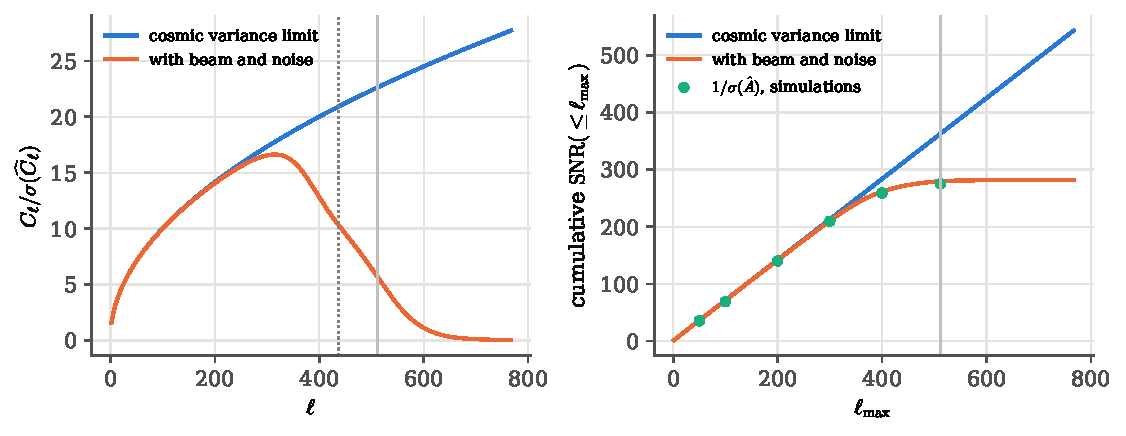
\includegraphics[width=12.5cm]{figures/ch08/snr.pdf}
\caption{Signal-to-noise of the toy experiment. Left: per multipole, against the
cosmic-variance limit $\sqrt{(2\ell+1)/2}$ (blue). The noise turns the curve over at
$\ell=\EightASnrPeakEll$, before the power equality $\ell_{\rm eq}$ (dotted); the grey line, in both panels, marks the analysed limit $\ell=512$. Right: cumulative, up to $\ell_{\max}$. Without noise it would keep
rising; with the beam and the noise it saturates. The green dots are $1/\sigma(\hat A)$ measured
on the simulated skies of \cref{8a:sec:results}.}
\label{8a:fig:snr}
\end{figure}
\section{The Monte Carlo machine}
\label{8a:sec:pipeline}

Three formulas now describe the full-sky estimator: its mean \eqref{8a:eq:cobs-mean}, its
variance \eqref{8a:eq:var} and its distribution \eqref{8a:eq:shifted-chi2}. Each was derived
under assumptions: a Gaussian sky, a circular beam, white noise, transforms that are exact on
the pixel grid. A simulation makes none of these assumptions on our behalf. It does to fake
skies exactly what the instrument and the analysis do to the real one, thousands of times,
and reads the statistics off the results. On the full sky the outcome must reproduce the
three formulas, and a disagreement means a mistake in a formula or in the code. Once the two
agree, the same machine can be pointed at the masked sky, where no formula is exact. This is
step~5 of the estimator recipe of \cref{ch:03}, carried out with the Monte Carlo tools of
\cref{ch:06}.

The question to answer before writing any code is: what must be simulated for the simulated
$\Chat$ to have the same distribution as the $\Chat$ we would compute from the real map? Two
kinds of ingredient enter the real $\Chat$. The random ones, the sky and the noise, must be
drawn afresh from their distributions for every simulated sky. The deterministic ones, the
beam, the pixels, the transforms, the noise subtraction and the deconvolution, must be applied
exactly as they would be to the data, with the same code. Anything left out of the simulation
is assumed to have no effect on $\Chat$.

\begin{workdef}[Monte Carlo of an observed spectrum]
For $i=1,\dots,N_{\rm sim}$, with independent random numbers each time:
\begin{enumerate}
  \item draw a Gaussian sky $\alm$ from the fiducial $\Cell$, up to $\ell=3N_{\rm side}-1$;
  \item multiply by the transfer function, $\alm\to T_\ell\alm$, and synthesise the map;
  \item add an independent Gaussian number of variance $\sigma_p^2$ to every pixel;
  \item analyse the map exactly as the data: transform, average $|d_{\ell m}|^2$ over $m$,
        subtract $N_\ell$, divide by $T_\ell^2$;
  \item store the spectrum $\widehat C^{(i)}_\ell$, not the map.
\end{enumerate}
\emph{Operationally:} the sample mean, sample variance and histogram of
$\{\widehat C^{(i)}_\ell\}$ estimate the mean, variance and distribution of $\Chat$
\unpack{to a precision set by $N_{\rm sim}$, which is itself computed, \cref{8a:sec:results}}.
\end{workdef}

\Cref{8a:fig:pipeline} draws the loop. Each step deserves the question: why is it
legitimate?

\begin{figure}[htbp]
\centering
\begin{tikzpicture}[
  bx/.style={draw=accent,thick,rounded corners=2pt,fill=ideabg,font=\small,
             minimum height=10mm,align=center,text width=24mm},
  rd/.style={bx,draw=fibreorange!80!black},
  flow/.style={->,thick,accent}]
  \node[bx] (cl)  at (0,0)     {fiducial $\Cell$\\ (CAMB)};
  \node[rd] (a)   at (3.4,0)   {1. draw\\ sky $\alm$};
  \node[bx] (t)   at (6.8,0)   {2. $T_\ell\alm$,\\ synthesise map};
  \node[rd] (n)   at (10.2,0)  {3. add pixel\\ noise $n_p$};
  \node[bx] (an)  at (10.2,-2.4) {4. transform,\\ $-N_\ell$, $/T_\ell^2$};
  \node[bx] (st)  at (6.8,-2.4)  {5. store\\ $\widehat C^{(i)}_\ell$};
  \node[bx] (sum) at (3.4,-2.4)  {mean, variance,\\ histogram};
  \draw[flow] (cl) -- (a); \draw[flow] (a) -- (t); \draw[flow] (t) -- (n);
  \draw[flow] (n) -- (an); \draw[flow] (an) -- (st); \draw[flow] (st) -- (sum);
  \draw[flow,dashed] (st.north) -- (a.south east);
  \node[font=\footnotesize,softgray!40!black,align=center] at (3.4,-3.55) {compare with
        \eqref{8a:eq:cobs-mean}, \eqref{8a:eq:var}, \eqref{8a:eq:shifted-chi2}};
  \node[font=\footnotesize,fibreorange!80!black,anchor=west] at (11.65,0) {random};
  \node[font=\footnotesize,accent,anchor=west] at (11.65,-2.4) {as for data};
\end{tikzpicture}
\caption{The Monte Carlo loop. The two orange steps draw random numbers, the sky and the
noise, afresh for every simulated sky. The blue steps are deterministic and identical to what
is done to the real map. The dashed line closes the loop; only the spectra leave it, and their
statistics are compared with the formulas of the previous sections.}
\label{8a:fig:pipeline}
\end{figure}

\paragraph{Step 1: the sky.}
A statistically isotropic Gaussian sky is completely specified by its spectrum
(\cref{ch:07}): the $\alm$ are independent, $a_{\ell0}\sim\Normal(0,\Cell)$ is real, and for
$m>0$ the real and imaginary parts are independent $\Normal(0,\Cell/2)$, with
$a_{\ell,-m}=(-1)^ma^*_{\ell m}$ fixing the negative $m$; after the rescaling of
\eqref{8a:eq:u-def} these are $2\ell+1$ independent $\Normal(0,\Cell)$ numbers. Drawing those numbers is therefore a
correct draw of a whole sky. We draw them with our own generator rather than
\pyname{healpy.synalm}, so that every random number goes through the reproducible stream
\pyname{rng_for("ch08", ...)} (\cref{ch:06}):
\pyfile[firstline=159,lastline=168,firstnumber=159]{code/ch08/lib_cmbsim.py}{Drawing one Gaussian sky}
Line~165 picks the standard deviation $\sqrt{\Cell}$ for every stored coefficient; line~168 uses
the real part alone for $m=0$ and divides the complex draw by $\sqrt2$ for $m>0$, so that
$\langle|\alm|^2\rangle=\Cell$ in both cases. With $\ell\le767$ there are
$768\times769/2=295\,296$ stored coefficients per sky.

\paragraph{Step 2: the instrument.}
The convolution theorem (\cref{8a:sec:beam}) makes the beam a multiplication of each $\alm$ by
$B_\ell$; the pixel window is applied the same way, as a factor $p_\ell$. The function
\pyname{observe_signal} is two lines: \pyname{almxfl} multiplies by $T_\ell=B_\ell p_\ell$, and
\pyname{alm2map} synthesises the $N_{\rm side}=256$ map. One simplification hides here. A real
map averages the beamed sky over each pixel, and HEALPix pixels have slightly different
shapes, so $p_\ell$ is only the sky-averaged effect \cite{Gorski2005}. Applying it as an exact
factor assumes every pixel has the average shape. The error this makes is far below the
precision of anything we measure, but a real pipeline that cared about it would simulate the
pointing and the pixelisation instead \srcref{Hivon}{§3.2}.

\paragraph{Step 3: the noise.}
Independent Gaussian pixel noise is drawn with the depth of the experiment,
$\sigma=\EightASigmaPix\,\mu$K per pixel. To test the cross-spectrum of \cref{8a:sec:cross} on
the same skies, each simulation draws two half-mission noise maps $n^{(1)},n^{(2)}$, each with
variance $2\sigma^2$ because each half has half the observing time. The full-mission noise is
their average, $(n^{(1)}+n^{(2)})/2$, of variance $\sigma^2$, which is exactly how co-adding two
halves of a real mission works. A further noise map with the pole-heavy variance pattern of
\cref{8a:sec:noise} tests inhomogeneous noise.

\paragraph{Step 4: the analysis.}
The map is transformed back with \pyname{healpy.map2alm} up to $\ell=512=2N_{\rm side}$, the
range in which the pixel quadrature reproduces the orthogonality of the $Y_{\ell m}$
(\cref{ch:07}). The transform of a pixel map is a quadrature, not an exact integral, and
healpy can refine it iteratively. Three iterations make the signal transform accurate to
about $10^{-5}$; for white noise, whose power fills every multipole up to the pixel scale, one
iteration already reproduces its spectrum to the Monte Carlo precision, so the noise maps use
one. Then \pyname{alm2cl} averages over $m$ and \pyname{debias} applies \eqref{8a:eq:chat}.

\paragraph{One sky, seven observations.}
The loop of \pyname{simulate} does all of this, and it observes each simulated sky in seven
ways at once:
\pyfile[firstline=229,lastline=246,firstnumber=229]{code/ch08/lib_cmbsim.py}{The Monte Carlo loop}
Lines 234--236 make one signal transform and two half-noise transforms. Because a transform is
linear, the full-mission noise needs no transform of its own (line~237), and every spectrum
in lines 238--242 is formed from these three sets of coefficients: the sky itself
(\pyname{sky}, cosmic variance only), the beamed sky without noise (\pyname{sig}), the
full-mission map (\pyname{auto}), the cross-spectrum of the two halves (\pyname{cross}) and the
noise alone (\pyname{noise}); lines 243--246 add the inhomogeneous noise with and without the
sky. All seven see the \emph{same} sky. When two estimators are compared on the same
simulated skies, the sky's own fluctuation is common to both and cancels in their difference,
so the difference is measured far more precisely than either one. This is the method of
\newterm{common random numbers}, and it is why the bias of the cross-spectrum relative to
the auto-spectrum can be measured to a fraction of a per cent with a few thousand skies
(\cref{8a:fig:seven}).

\begin{figure}[htbp]
\centering
\begin{tikzpicture}[
  bx/.style={draw=accent,thick,rounded corners=2pt,fill=ideabg,font=\small,
             minimum height=8mm,align=center,text width=21mm},
  sp/.style={draw=black!35,rounded corners=2pt,fill=white,font=\scriptsize,
             minimum height=6.5mm,align=center,text width=38mm},
  flow/.style={->,thick,accent}]
  \node[bx] (a)  at (0,0)     {one sky $\alm$};
  \node[bx] (s)  at (3.2,1.2) {$T_\ell\alm$\\ (signal map)};
  \node[bx] (n)  at (3.2,-1.2) {noise $n^{(1)},n^{(2)}$,\\ $n^{\rm inh}$};
  \node[sp] (o1) at (8.8,3.0)  {\pyname{sky}: $|\alm|^2$};
  \node[sp] (o2) at (8.8,2.0)  {\pyname{sig}: $T^2|a|^2$};
  \node[sp] (o3) at (8.8,1.0)  {\pyname{auto}: $s+\bar n$};
  \node[sp] (o4) at (8.8,0.0)  {\pyname{cross}: $(s{+}n^{(1)})(s{+}n^{(2)})$};
  \node[sp] (o5) at (8.8,-1.0) {\pyname{noise}: $\bar n$ alone};
  \node[sp] (o6) at (8.8,-2.0) {\pyname{inh}: $s+n^{\rm inh}$};
  \node[sp] (o7) at (8.8,-3.0) {\pyname{ninh}: $n^{\rm inh}$ alone};
  \draw[flow] (a) -- (s); \draw[flow] (a) -- (n);
  \draw[flow] (a.north) |- (o1.west);
  \foreach \k in {o2,o3,o4,o6}{\draw[flow,formblue!60] (s.east) -- (\k.west);}
  \foreach \k in {o3,o4,o5,o6,o7}{\draw[flow,fibreorange!70] (n.east) -- (\k.west);}
\end{tikzpicture}
\caption{Each simulated sky is observed seven ways. Blue lines carry the beamed signal,
orange lines the noise; a spectrum fed by both lines contains both. Because the seven spectra
share one sky, comparisons between them are free of the sky's own fluctuation.}
\label{8a:fig:seven}
\end{figure}

\paragraph{The driver script.}
The run itself is a short script:
\pyfile[firstline=11,lastline=40,firstnumber=11]{code/ch08/05_mc_run.py}{Running and caching the full-sky Monte Carlo}
The function \pyname{cs.cached} runs \pyname{make()} once and writes the seven arrays of spectra
to the file \pyname{mc_fullsky.npz} in \pyname{data/ch08/}; every later call reads them back, so the analysis
scripts \pyname{06}--\pyname{10} and \pyname{12} all work on the same skies without recomputing
them. The run took $\EightAMinutes$ minutes, $\EightASecPerSky$\,s per sky, for
$N_{\rm sim}=\EightANsim$.

\paragraph{Example: what the run stores.}
Seven spectra of $513$ multipoles in single precision, for $2000$ skies, occupy
$7\times513\times4\times2000\approx29$\,MB. The maps themselves would be $786\,432$ pixels in
double precision, $6.3$\,MB each, or $88$\,GB for seven maps of $2000$ skies. Storing spectra and
not maps is what makes the run fit on a laptop disk; any statistic of $\Chat$ can still be
computed later.

\paragraph{Example: how many skies to plan for.}
The number of simulations is chosen before the run, from what is to be measured. An error bar
estimated from $N$ simulations has a relative Monte Carlo error of $1/\sqrt{2(N-1)}$ (the
sampling error of a standard deviation, \cref{ch:03}), so $10\%$ needs
$N=1+1/(2\times0.1^2)=\EightANTenPct$ skies. A bias is harder. In a bin of $25$ multipoles
around $\ell=400$, one simulated estimate scatters by $\EightASigBin\%$, and the mean of $N$ of
them by $\EightASigBin\%/\sqrt N$; to see a bias of $0.1\%$ at one standard deviation needs
$N=(\EightASigBin/0.1)^2\approx\EightANOnePermil$ skies. The $\EightANsim$ skies of the run
resolve a bias of about $0.04\%$ per bin.

\paragraph{Example: why $N_{\rm side}=256$.}
The resolution must be fine enough to show both regimes of the problem, the
cosmic-variance-limited one and the noise-limited one. With a $30'$ beam and
$200\,\mu$K\,arcmin, the noise takes over at $\ell_{\rm eq}=\EightALeq$, inside the trusted
range $\ell\le512$ of $N_{\rm side}=256$, so this resolution is enough. One pair of
transforms there takes $\EightAScaleTwoFiveSix$\,s on this laptop. The cost grows as
$N_{\rm pix}^{3/2}\propto N_{\rm side}^3$: $\EightAScaleFiveTwelve$\,s at $N_{\rm side}=512$,
$\EightAScaleTenTwentyFour$\,s at $1024$, and an extrapolated $\EightAScaleTwentyFortyEight$\,s at
$2048$, the Planck resolution.

\paragraph{What the laptop version gives up.}
Each choice above is a reduction of what a research analysis does, and each has a price.
\begin{itemize}
  \item \emph{Resolution.} Planck analyses its temperature maps at $N_{\rm side}=2048$ up to
        $\ell\approx2500$ \cite{Planck2018V}; we use $N_{\rm side}=256$ and $\ell\le512$. At the same
        $\EightANsim$ skies that would take about $\EightAScaleSkySec$\,s per sky, roughly ten hours
        of the laptop's full processor instead of six minutes, and $\EightAScaleMapGB$\,GB per map.
        The cut keeps $\EightAScaleModeFrac\%$ of the harmonic modes, so a cosmic-variance-limited
        amplitude would be measured $\EightAScaleSNRloss$ times less precisely; the beam was
        widened to match, so the two regimes of the problem, and every statement about them, are
        unchanged.
  \item \emph{Number of simulations.} The Planck 2018 likelihood analysis validates its
        spectra with, and builds its low-$\ell$ polarisation likelihood from, $300$ end-to-end
        simulations of the full mission (FFP10) \cite{Planck2018V}; we use $\EightANsim$ Gaussian
        skies. An error bar from $300$ simulations carries a Monte Carlo error of
        $\EightAScaleMCerrThree\%$, ours $\EightAScaleMCerrTwoK\%$. We can afford more because each of
        ours is cheap, and we pay for it in realism.
  \item \emph{Realism of a simulated sky.} An end-to-end simulation generates the timestream
        of every detector along the real scan, with correlated $1/f$ noise, and runs the
        real map-maker on it \srcref{Hivon}{§3.2--3.3}; we draw the noise directly in pixels, white
        and uncorrelated. Our simulations can therefore test only what this model contains: the
        stripes, the filtering and the noise correlations of a real map are absent.
  \item \emph{Beam.} Real effective beams are measured on planets, are not circular, and
        carry their own uncertainty; ours is an exact circular Gaussian. Suppose the beam used in
        the analysis is wrong by a small fraction $\epsilon=\delta B_\ell/B_\ell$. The estimator
        $\Chat=(\widehat C^{\,\rm obs}_\ell-N_\ell)/T_\ell^2$ then divides by $B_\ell^2(1+\epsilon)^2$
        instead of $B_\ell^2$, which multiplies the estimate by $(1+\epsilon)^{-2}\approx1-2\epsilon$:
        a relative bias of $-2\,\delta B_\ell/B_\ell$, an effect this pipeline cannot show.
\end{itemize}
\Cref{8a:sec:research} sets these choices beside the full analysis step by step.
\section{What the simulations show}
\label{8a:sec:results}

The run of \cref{8a:sec:pipeline} produced $\EightANsim$ simulated skies of the toy
experiment: a $30'$ Gaussian beam, $N_{\rm side}=256$ pixels, $200\,\mu$K\,arcmin of white
noise, the Planck 2018 fiducial spectrum. Each sky was observed seven ways and its spectra
were stored up to $\ell=512$. Every formula of the previous sections makes a definite
prediction for these numbers. We now take the predictions one at a time, in the order of the
sub-questions of \cref{8a:sec:problem}: the mean, the width, the shape, and the number of
simulations it took to know.

\subsection{The mean: is the bias gone?}
\label{8a:sec:res-bias}

The left panel of \cref{8a:fig:bias} plots the average over the simulations of the raw
observed spectrum $\widehat C^{\,\rm obs}_\ell$, the average of $|d_{\ell m}|^2$ over $m$ on the
noisy map. It lies on the prediction $T_\ell^2\Cell+N_\ell$ of \eqref{8a:eq:cobs-mean} at every
multipole: on the beamed sky $T_\ell^2\Cell$ at low $\ell$, on the flat noise $N_\ell$ at high
$\ell$. The noise-only maps give the noise power directly, and their average over all
multipoles and all simulations is $\EightANlRatio\pm\EightANlRatioErr$ times
$\sigma^2\Omega_{\rm pix}$, confirming \eqref{8a:eq:nl}.

\begin{figure}[htbp]
\centering
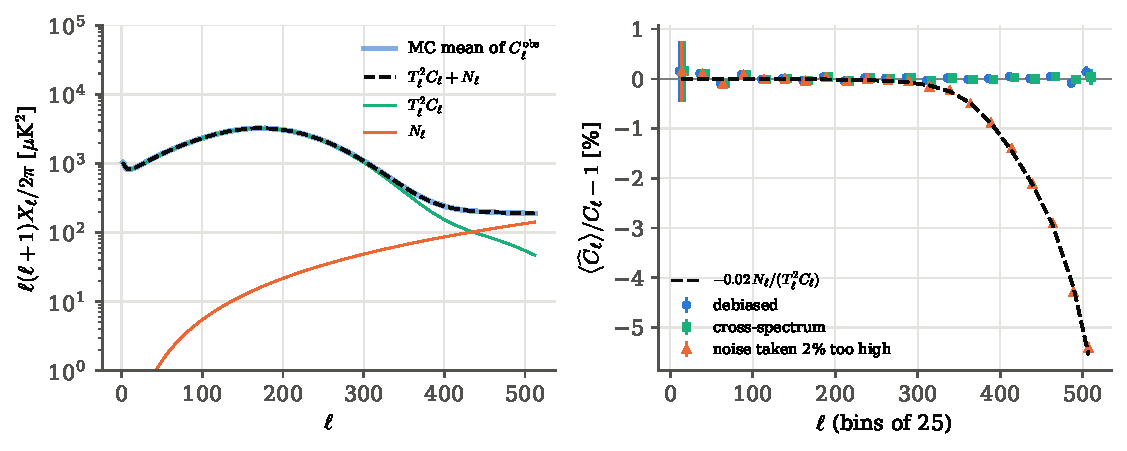
\includegraphics[width=12.5cm]{figures/ch08/bias.pdf}
\caption{The mean of the estimators over $\EightANsim$ simulated skies. Left: the raw observed
spectrum (blue) follows $T_\ell^2\Cell+N_\ell$ (dashed), the sum of the beamed sky (green) and the
noise (orange). Right: the fractional bias in bins of $25$ multipoles. The debiased
estimator (blue) and the cross-spectrum of the two half maps (green) scatter around zero within
their Monte Carlo error bars. Subtracting a noise level that is $2\%$ too high (orange) produces
the negative bias predicted by \eqref{8a:eq:noise-error} (dashed).}
\label{8a:fig:bias}
\end{figure}

The real test is the debiased estimator \eqref{8a:eq:chat}, plotted as a fractional bias in
$\EightANbins$ bins of $25$ multipoles in the right panel. Its points scatter around zero, the
largest by $\EightAMaxAbsBias\%$, with typical Monte Carlo error bars of $\EightATypBiasErr\%$.
Is that zero? Say what was observed: $\EightANbins$ small deviations from zero, each measured
with a known Monte Carlo error. What could have produced them? Either the estimator is
unbiased and the deviations are the fluctuation of a finite set of simulations, or there is a
real bias. Only the first hypothesis predicts how large the deviations should be, so it is
the null hypothesis of \cref{ch:04}: if it is true, each deviation divided by its error is a
standard Gaussian, and the sum of their squares is a $\chi^2$ variable with $\EightANbins$
degrees of freedom. The observed sum is $\EightAChiAuto$. The question is then whether a value
this large, or larger, would be unremarkable if there were no bias, and the answer is yes:
the probability is $p=\EightAPAuto$. The simulations see no bias at the level of
$\EightATypBiasErr\%$ per bin. The cross-spectrum, with no noise subtracted at all, passes the
same test with $\chi^2=\EightAChiCross$ ($p=\EightAPCross$), as \eqref{8a:eq:cross} predicted.

\paragraph{Example: three ways to get it wrong.}
The same simulations show what the corrections are worth, because the wrong estimators can
be computed from the same stored spectra.
\begin{itemize}
  \item \emph{No noise subtraction.} The bias is $+\EightANoSubBiasFirst\%$ in the first bin,
        where the noise is negligible, and $+\EightANoSubBiasLast\%$ in the last, close to the
        $N_\ell/(T_\ell^2\Cell)\approx\EightANoverSlmax$ of \cref{8a:sec:noise-bias}.
  \item \emph{Pixel window forgotten.} Dividing by $B_\ell^2$ instead of $B_\ell^2p_\ell^2$ leaves
        the factor $p_\ell^2$ in the estimate. In the last bin that is a bias of
        $\EightAPixForgotLast\%$, the $32\%$ power suppression computed in \cref{8a:sec:beam}.
  \item \emph{Noise level $2\%$ too high.} The last bin is biased by $\EightAMisLast\%$; the
        prediction $-0.02\,N_\ell/(T_\ell^2\Cell)$ of \eqref{8a:eq:noise-error}, averaged over the
        bin, is $\EightAMisPredLast\%$.
\end{itemize}

\subsection{The width: does the variance follow the formula?}
\label{8a:sec:res-var}

For each multipole, divide the sample variance of the $\EightANsim$ simulated $\Chat$ by the
prediction \eqref{8a:eq:var}. If the formula is right, the ratio is one up to Monte Carlo
error. How large is that error? For Gaussian draws the sample variance of $n$ of them is a
scaled $\chi^2_{n-1}$, and the variance $2(n-1)$ of that $\chi^2$ gives it a relative error
$\sqrt{2/(n-1)}$ \eqref{7b:eq:var-s2-gauss}. A heavier tail than the Gaussian makes occasional draws
large, and their squares then move the sample variance further; the fourth moment enters, and the
relative error becomes $\sqrt{2/(n-1)+\kappa/n}$, with $\kappa$ the excess kurtosis of one draw
\eqref{7b:eq:var-s2-kurt}. Our draws are values of $\Chat$, a scaled and shifted $\chi^2_\nu$, so
$\kappa=12/\nu$ by \eqref{8a:eq:chi2-shape}. With $\nu=2\ell+1$ this is negligible except at the
lowest multipoles; at $\ell=100$ the expected spread of the ratio is $\EightASpreadOne\%$.

\begin{figure}[htbp]
\centering
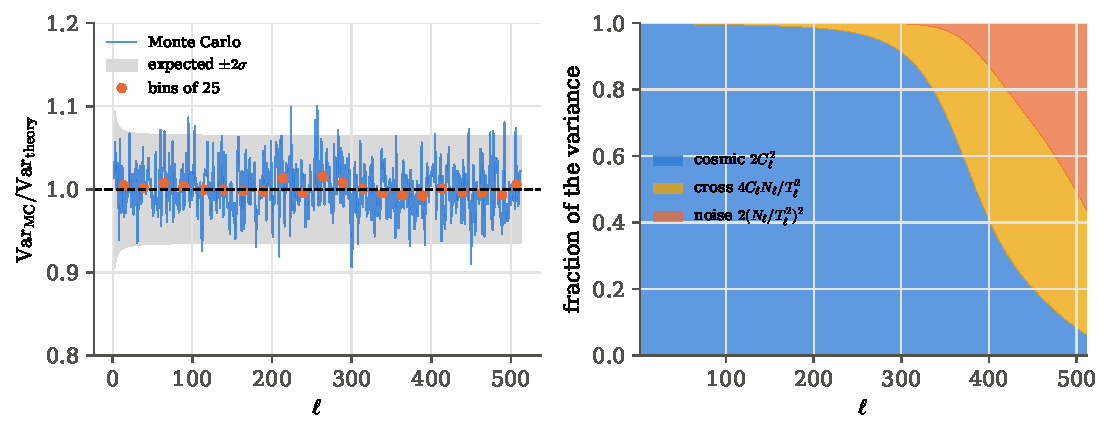
\includegraphics[width=12.5cm]{figures/ch08/variance.pdf}
\caption{The scatter of the debiased estimator. Left: Monte Carlo variance divided by the
prediction $2(\Cell+N_\ell/T_\ell^2)^2/(2\ell+1)$ at every multipole (blue), with the band in
which $95\%$ of the points should fall (grey) and bin averages (orange). Right: the share of
the three terms of \eqref{8a:eq:var-terms} in the variance. The cosmic variance (blue) gives way
to the sky--noise cross term (yellow) and then to the pure noise term (orange).}
\label{8a:fig:variance}
\end{figure}

The left panel of \cref{8a:fig:variance} shows the result. Averaged over $\ell=2$--$512$, the
ratio is $\EightAVarRatio\pm\EightAVarRatioErr$. The sum of the squared standardised deviations is
$\EightAVarChi$ for $\EightAVarDof$ multipoles ($p=\EightAVarPval$), and $\EightAVarFracOut\%$ of the
multipoles fall outside the two-standard-deviation band, against the $4.6\%$ expected. The
sky-only spectra, observed with no instrument, give a variance ratio of $\EightACVRatio$ against
the cosmic variance of \cref{ch:07}. The right panel splits the prediction into the three terms
of \eqref{8a:eq:var-terms}. At $\ell=512$ the pure noise term carries $\EightANoiseFracLmax\%$ of
the variance and the cross term $\EightACrossFracLmax\%$; the noise terms pass half of the total at
$\ell=\EightALHalfNoiseVar$, the multipole where $r_\ell=\sqrt2-1$.

\paragraph{Example: the price of the cross-spectrum.}
\Cref{8a:sec:cross} predicted that the cross-spectrum of two half maps, which needs no noise
model, scatters more than the auto-spectrum, by the factor
$\sqrt{[(S+2N)^2+S^2]/[2(S+N)^2]}$ with $S=T_\ell^2\Cell$ and $N=N_\ell$. Because both estimators
are computed on the same simulated skies, the ratio of their scatters is measured with the
sky's fluctuation cancelled. \Cref{8a:fig:cross} shows it following the prediction from $1$ at
low $\ell$ towards $\sqrt2$; at the top of the band the predicted factor is
$\EightACrossRatioLmax$ and the simulations give $\EightACrossRatioMCLast$.

\begin{figure}[htbp]
\centering
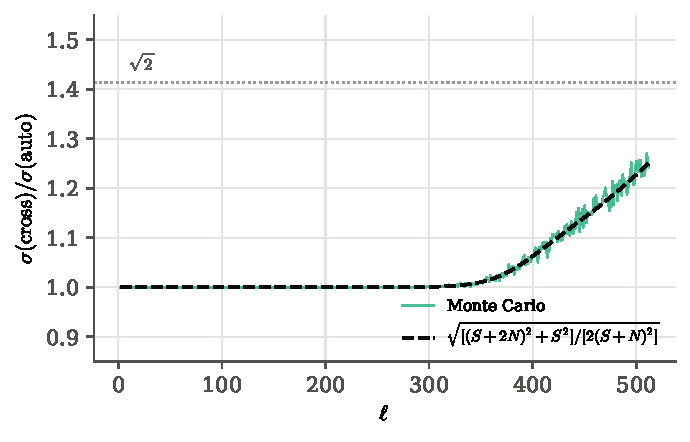
\includegraphics[width=8.5cm]{figures/ch08/cross.pdf}
\caption{Scatter of the cross-spectrum of two half maps divided by that of the auto-spectrum
of the full map, on the same simulated skies (green), and the prediction (dashed). The ratio
is one where the sky dominates and climbs towards $\sqrt2$ (dotted) where the noise does.}
\label{8a:fig:cross}
\end{figure}

\paragraph{Example: the amplitude of the whole spectrum.}
The cumulative signal-to-noise of \cref{8a:sec:snr} predicts that the inverse-variance
weighted amplitude $\hat A$ of \eqref{8a:eq:amp}, built from all multipoles up to $512$, has an
error $1/\SNR(\le512)=\EightASigAth$. On the simulated skies its scatter is $\EightASigAmc$, with a
Monte Carlo error of $\EightASigAerr\%$, and its mean is $\EightAMeanA\pm\EightAMeanAerr$. The
points in the right panel of \cref{8a:fig:snr} repeat the comparison for other $\ell_{\max}$.

\subsection{The shape: shifted $\chi^2$ or Gaussian?}
\label{8a:sec:res-shape}

\Cref{8a:fig:histograms} compares the histograms of $\Chat/\Cell$ at four multipoles with the
shifted, scaled $\chi^2$ of \eqref{8a:eq:shifted-chi2} and with a Gaussian of the same mean and
width. The Kolmogorov--Smirnov test of \cref{ch:04} measures the largest distance between the
cumulative distribution of the simulations and that of a model; its $p$-values for the shifted
$\chi^2$ are $\EightAKSthree$, $\EightAKSthirty$, $\EightAKSleq$ and $\EightAKSlmax$ at $\ell=3$, $30$,
$\EightALeq$ and $512$, none of them small. At $\ell=3$ the measured skewness is $\EightASkewThree$,
the $\chi^2_7$ value is $\EightASkewThreeTh$, and the Gaussian, which has no skewness, is rejected
with $p=\EightAHivKSgauss$. By $\ell=30$ the two models are hard to tell apart by eye, and by
$\ell_{\rm eq}$ they coincide.

\begin{figure}[htbp]
\centering
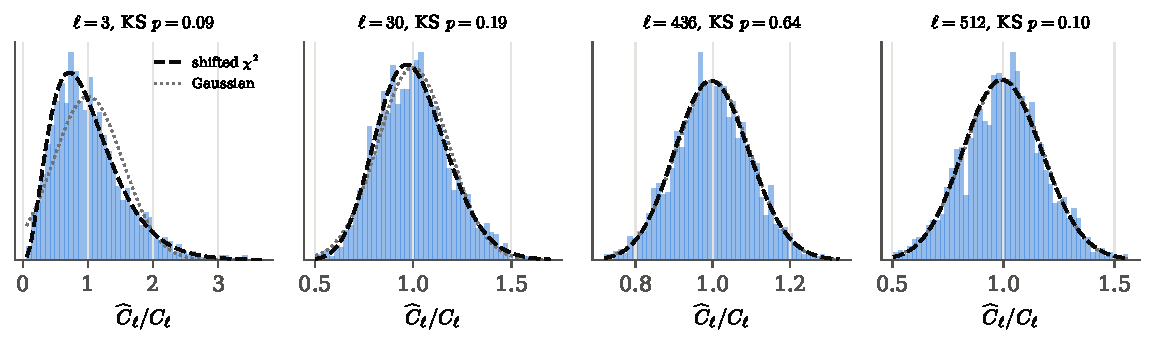
\includegraphics[width=12.5cm]{figures/ch08/histograms.pdf}
\caption{Histograms of $\Chat/\Cell$ over the simulated skies at four multipoles, with the
shifted $\chi^2$ (dashed) and the Gaussian of the same mean and width (dotted). At $\ell=3$ the
distribution is strongly skewed and only the $\chi^2$ follows it; at higher $\ell$ the two
models merge.}
\label{8a:fig:histograms}
\end{figure}

\subsection{When the noise is not uniform}
\label{8a:sec:res-inh}

Real scans revisit some parts of the sky more often than others. The simulations include a
noise map whose pixel variance follows the pattern $\sigma_p^2\propto1/(1+4\cos^2\theta)$, the
inverse of a hit count that is five times larger at the poles than at the equator, normalised
so that its sky average equals the uniform $\sigma^2$. The relative variance then runs from
$\EightAInhVmin$ at the poles to $\EightAInhVmax$ at the equator (\cref{8a:fig:inh}, left).

Two predictions were made in \cref{8a:sec:noise}. The \emph{bias} is $\Omega_{\rm pix}$ times
the mean pixel variance \eqref{8a:eq:nbar}, whatever the pattern: the simulations give
$\EightAInhBias\pm\EightAInhBiasErr$ times the uniform value. The \emph{scatter} depends on the full
pattern. For the noise alone, write its harmonic covariance
$N_{mm'}\equiv\langle n_{\ell m}n^*_{\ell m'}\rangle$ at fixed $\ell$, from
\eqref{8a:eq:noise-cov-general}. A pattern that depends only on $\theta$ does not couple
different $m$, because the $\phi$ integral of $e^{i(m'-m)\phi}$ vanishes, so $N_{mm'}=\delta_{mm'}N_{mm}$.
The modes are still independent Gaussians, but with different variances $N_{mm}$, and
\begin{align}
  \Var\Bigl(\frac{1}{2\ell+1}\sum_m|n_{\ell m}|^2\Bigr)
  &\eqby{1}\frac{2}{(2\ell+1)^2}\sum_mN_{mm}^2
  \nonumber\\
  &\relby{2}{\ge}\frac{2}{(2\ell+1)^3}\Bigl(\sum_mN_{mm}\Bigr)^2
   \eqby{3}\frac{2\,\bar N_\ell^2}{2\ell+1} .
  \label{8a:eq:var-inh}
\end{align}
\begin{explain}
  \item Each of the $2\ell+1$ real degrees of freedom of mode $m$ is Gaussian with variance set
        by $N_{mm}$, so, as in \eqref{8a:eq:var}, each contributes $2N_{mm}^2$; the reality
        condition $n_{\ell,-m}=(-1)^mn^*_{\ell m}$ pairs $m$ with $-m$ and is already counted in the
        sum over all $m$.
  \item Cauchy--Schwarz, $\bigl(\sum_m1\cdot N_{mm}\bigr)^2\le(2\ell+1)\sum_mN_{mm}^2$.
  \item $\bar N_\ell=\sum_mN_{mm}/(2\ell+1)$ is the average noise power of \eqref{8a:eq:nbar}.
\end{explain}
The right-hand side is the white-noise variance with the same mean power. Non-uniform noise
therefore never decreases the scatter at fixed bias, and increases it by the factor
$(2\ell+1)\sum_mN_{mm}^2/(\sum_mN_{mm})^2$, a measure of how unequal the mode variances are.
Script \pyname{09_inhomogeneous.py} computes $N_{mm}$ exactly for our pattern from
\eqref{8a:eq:noise-cov-general}, ring by ring, and predicts a factor $\EightAInhVarNoisePred$
above $\ell=100$; the simulations give $\EightAInhVarNoise$. With the sky added, each mode has
variance $T_\ell^2\Cell+N_{mm}$, the prediction becomes $\sum_m(T_\ell^2\Cell+N_{mm})^2$ over its
uniform value, $\EightAInhVarTotPredLmax$ at $\ell=512$, and the simulations give
$\EightAInhVarTotLmax$; below $\ell=100$, where the sky dominates, the ratio is
$\EightAInhVarTotLow$.

\begin{figure}[htbp]
\centering
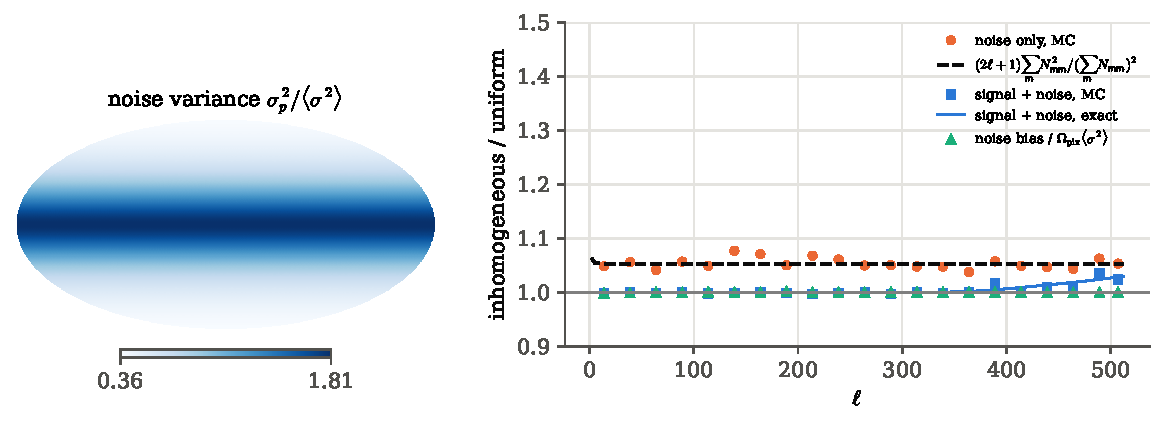
\includegraphics[width=12.5cm]{figures/ch08/inhomogeneous.pdf}
\caption{Inhomogeneous noise. Left: the relative pixel noise variance of the simulated scan,
low at the well-observed poles. Right: inhomogeneous over uniform noise, for the noise bias
(green, equal to one), the scatter of the noise spectrum (orange points against the exact
prediction, dashed) and the scatter of the full spectrum (blue). The scatter rises by a few per
cent only, because each harmonic mode averages the noise over a large part of the sky.}
\label{8a:fig:inh}
\end{figure}

\paragraph{Example: why the increase is only five per cent.}
A naive guess would be that the variance of the noise spectrum grows like the sky average of
$\sigma_p^4$ over $\langle\sigma^2\rangle^2$, which for this pattern is $\EightAInhVsq$. The exact
factor $(2\ell+1)\sum_mN_{mm}^2/(\sum_mN_{mm})^2$ is much closer to one, because $N_{mm}$ is not a
pixel variance. By \eqref{8a:eq:noise-cov-general} it is
$N_{mm}=\Omega_{\rm pix}^2\sum_p\sigma_p^2|Y_{\ell m}(\hat{\bm n}_p)|^2$: the pixel variance weighted by
the mode's own $|Y_{\ell m}|^2$, which integrates to one over the sky, so each $N_{mm}$ is
$\Omega_{\rm pix}$ times an average of $\sigma^2$ over the sky. Measure $\sigma^2$ in units of its sky
mean, $\sigma^2(\theta)=c/(1+4\cos^2\theta)$ with $c=\EightAInhVmax$, and let $x=\cos\theta$.
\begin{itemize}
  \item The $m=0$ mode spreads along whole meridians: averaged over its oscillations, $|Y_{\ell0}|^2$
        weights $x$ by $1/(\pi\sqrt{1-x^2})$, which reaches the poles. Writing $x=\sin\phi$ turns the
        average into $\frac1\pi\int_0^\pi c\,\dd\phi/(1+4\sin^2\phi)=c/\sqrt5$, so
        $N_{00}\approx0.81$ in these units, although the pole pixels themselves have $\EightAInhVmin$.
  \item The $|m|=\ell$ modes are confined to a narrow band around the equator, so they see only the
        equatorial value, $N_{\ell\ell}\approx c=\EightAInhVmax$.
  \item In between, a mode with $\mu=|m|/\ell$ reaches up to $|x|=\sqrt{1-\mu^2}$, and the same average
        gives $N_{mm}\approx c/\sqrt{5-4\mu^2}$.
\end{itemize}
So the mode variances run only from $0.81$ to $1.81$, while the pixel variances run from
$\EightAInhVmin$ to $\EightAInhVmax$. For large $\ell$ the $m$ are spread evenly in $\mu$, the sums
over $m$ become integrals over $\mu$, and
\[
  \frac{(2\ell+1)\sum_mN_{mm}^2}{\bigl(\sum_mN_{mm}\bigr)^2}
  \approx\frac{\int_0^1c^2\,\dd\mu/(5-4\mu^2)}{\bigl[\int_0^1c\,\dd\mu/\sqrt{5-4\mu^2}\bigr]^2}
  =\frac{3.262\times0.323}{1^2}=1.053 ,
\]
the denominator being one because the average of $N_{mm}$ over $m$ is the sky mean
\eqref{8a:eq:nbar}. This is the exact prediction $\EightAInhVarNoisePred$ quoted above. The naive
$\langle\sigma^4\rangle/\langle\sigma^2\rangle^2$ is larger because it treats every pixel as a separate
mode with its own variance; a harmonic mode instead averages many pixels, quiet and noisy together,
and only the leftover difference between polar-reaching and equatorial modes counts.

\subsection{How many simulations did it take?}
\label{8a:sec:res-conv}

The last sub-question of \cref{8a:sec:problem} is about the method itself. \Cref{8a:fig:conv}
follows the estimates in one bin, $\ell=400$--$424$, as the number of simulated skies $N$
grows. The running estimate of the bias wanders inside the envelope $\pm\sigma/\sqrt N$, with
$\sigma=\EightASigBin\%$ the scatter of one binned estimate. The relative error of the estimated
error bar, measured as the spread over $200$ random reorderings of the skies, falls as
$1/\sqrt{2(N-1)}$: at $N=\EightARelErrNval$ it is $\EightARelErrN\%$, against the predicted
$\EightARelErrNth\%$. An error bar good to $10\%$ needs about $\EightANTenPct$ skies, a bias
measured to $0.1\%$ about $\EightANOnePermil$.

\begin{figure}[htbp]
\centering
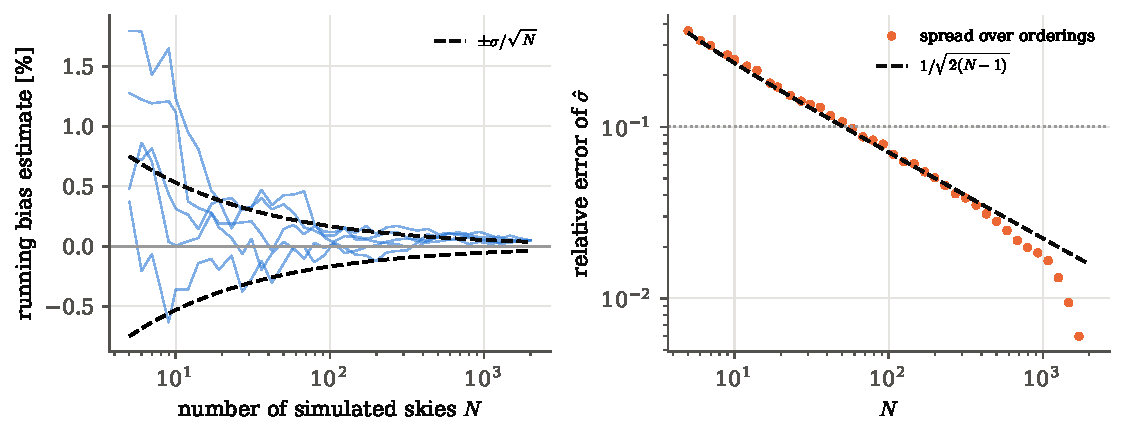
\includegraphics[width=12.5cm]{figures/ch08/convergence.pdf}
\caption{Convergence with the number of simulations, in the bin $\ell=400$--$424$. Left: five
running estimates of the fractional bias, each from a different ordering of the skies, inside
the $\pm\sigma/\sqrt N$ envelope (dashed). Right: the relative error of the estimated error bar,
from the spread over $200$ orderings (points), and $1/\sqrt{2(N-1)}$ (dashed); the dotted line
marks $10\%$. Near the $2000$ skies available the points drop below the line, because every
ordering then draws nearly the same skies.}
\label{8a:fig:conv}
\end{figure}

\begin{keyidea}[The full-sky verdict]
On the full sky with a beam, a pixel window and white or inhomogeneous noise, the simulations
reproduce the bias \eqref{8a:eq:cobs-mean}, the variance \eqref{8a:eq:var}, the distribution
\eqref{8a:eq:shifted-chi2} and the inhomogeneous-noise scatter \eqref{8a:eq:var-inh}, each to its
Monte Carlo precision. The machine is therefore trusted where no formula exists.
\end{keyidea}
\section{Reproducing the literature}
\label{8a:sec:literature}

Two papers set up the full-sky problem. \textcite{Knox1995} wrote down the error bar
of a spectrum measured from a full-sky map with a Gaussian beam and white noise, and used it
to forecast what a satellite could learn about inflation. \textcite{Hivon2002} built the
MASTER method, the pseudo-$\Cell$ estimator calibrated by Monte Carlo, and tested it on
simulated observations of the Boomerang balloon. Both papers quote numbers that our code
can recompute. Agreement is the check that the machine of \cref{8a:sec:pipeline} measures
what the field measures; a disagreement has to be explained, not ignored.

\subsection{Knox (1995): the error bar of a beamed, noisy map}
\label{8a:sec:lit-knox}

\paragraph{His question.}
In 1995 COBE had measured the large-angle anisotropy, and satellites that would map the whole sky
at much finer resolution were being proposed. Their promise was to measure $\Cell$ out to
$\ell\sim1000$, and through it the shape of the primordial spectrum that inflation predicts. Knox
asked how well such a map could actually pin down $\Cell$, given that any real instrument blurs
the sky with a beam of finite width and adds detector noise. He wanted one formula that gives the
error bar at every $\ell$ from a few numbers describing the instrument, so that designs could be
compared before any of them was built.

\paragraph{His setup.}
Four ingredients enter, and each has a plain meaning.
\begin{itemize}
  \item \emph{The sky.} A Gaussian random field with a spectrum $\Cell$ from a cosmological model.
        Knox used the standard cold-dark-matter model of the time, normalised to the quadrupole
        COBE measured; we use the Planck 2018 best fit (\cref{8a:tab:knox-setup}).
  \item \emph{The beam.} The telescope sees each direction blurred by a Gaussian beam, given by
        its full width at half maximum (FWHM).
  \item \emph{The pixel noise.} The map is stored in pixels of solid angle $\Omega_{\rm pix}$, and
        each pixel carries detector noise of standard deviation $\sigma_{\rm pix}$, independent from
        pixel to pixel. For a year of observation he took $\sigma_{\rm pix}=22\,\mu$K in
        $20'\times20'$ pixels \srcref{Knox1995}{p.~7}.
  \item \emph{The sky fraction.} A satellite sees the whole sky, $\fsky=1$.
\end{itemize}
What he forecasts is the standard deviation $\Delta\Cell$ of the estimated spectrum at each
$\ell$, and from it the errors on the inflationary parameters. The noise of a pixel and its size
combine into one number, $w^{-1}=\sigma_{\rm pix}^2\Omega_{\rm pix}$: a pixel twice as large has
half the noise variance per unit area, so only this product matters. For his satellite
$w^{-1}=22^2\times(1/3)^2\,\mu{\rm K}^2\,{\rm deg}^2$, so $w^{-1/2}=\EightAKnoxWinv\,\mu$K\,deg; he
quotes $7.5$, the same number to the precision of his $\sigma_{\rm pix}$.

\begin{table}[htbp]
\centering
\small
\renewcommand{\arraystretch}{1.2}
\begin{tabular}{@{}>{\raggedright\arraybackslash}p{3.0cm}>{\raggedright\arraybackslash}p{4.6cm}>{\raggedright\arraybackslash}p{4.4cm}@{}}
\hline
 & Knox (1995) & ours \\
\hline
cosmology & standard CDM: $h=0.5$, $\Omega_bh^2=0.0125$, no $\Lambda$, $n_S=0.94$, tensors $r=0.28$, COBE-normalised \srcref{Knox1995}{p.~4--5} & Planck 2018 best fit \\
sky fraction & $1$ & $1$ \\
pixel noise & $22\,\mu$K in $20'\times20'$ pixels & the same \\
noise weight $w^{-1/2}$ & $7.5\,\mu$K\,deg & $\EightAKnoxWinv\,\mu$K\,deg \\
beam FWHM & $20'$ & $20'$ \\
Fig.~2 experiments & $20'$ and $40'$, $w^{-1/2}=15$ and $30\,\mu$K\,deg & the same; maps for $w^{-1/2}=15$ \\
\hline
\end{tabular}
\caption{Knox's experiment and ours. Only the cosmology differs.}
\label{8a:tab:knox-setup}
\end{table}

\paragraph{The sky rms, and the signal-to-noise per pixel.}
How large is the signal in one pixel, compared with the noise? Knox gives the rms of the sky seen
through his $20'$ beam as $92.5\,\mu$K. It follows in three moves. The temperature in direction
$\hat{\bm n}$ is the beamed sum of the harmonics, $T(\hat{\bm n})=\sum_{\ell m}B_\ell\alm Y_{\ell m}(\hat{\bm n})$
by the convolution theorem \eqref{8a:eq:convolution}. The map is real, so $T^2=TT^*$, and
\begin{equation}
  \langle T^2\rangle
  \eqby{1}\sum_{\ell m}\sum_{\ell'm'}B_\ell B_{\ell'}\,\langle\alm a^*_{\ell'm'}\rangle\,
     Y_{\ell m}(\hat{\bm n})Y^*_{\ell'm'}(\hat{\bm n})
  \eqby{2}\sum_\ell B_\ell^2\Cell\sum_m|Y_{\ell m}(\hat{\bm n})|^2
  \eqby{3}\sum_\ell\frac{(2\ell+1)\,\Cell\,W_\ell}{4\pi},
  \nonumber
\end{equation}
\begin{explain}
  \item Multiply the sum by its complex conjugate and average over skies; only the $\alm$ are random.
  \item Different $(\ell,m)$ are uncorrelated and $\langle|\alm|^2\rangle=\Cell$, so only $\ell'=\ell$,
        $m'=m$ survives.
  \item The addition theorem $\sum_m|Y_{\ell m}|^2=(2\ell+1)/4\pi$, used in \eqref{8a:eq:nbar}; Knox
        writes the beam window $B_\ell^2$ as $W_\ell$.
\end{explain}
The direction has dropped out: every pixel has the same signal variance. Our fiducial spectrum
gives $\langle T^2\rangle^{1/2}=\EightAKnoxRms\,\mu$K (script \pyname{11_knox_reproduction.py}). Divided
by the noise per pixel, his rms gives $92.5/22=4.2$, the ``signal-to-noise of about 4 per pixel''
he quotes; ours gives $\EightAKnoxSnrPix$. The number says that the map is signal-dominated pixel by
pixel, but not by a wide margin: the noise is a quarter of the signal. Most of the pixel rms comes
from the large scales, so at the small scales the beam has already turned down, the noise takes
over, and that is why the beam and the noise set the error bars at high $\ell$. That two such
different cosmologies give rms values within a few per cent is a consequence of both being
normalised to the measured large-scale amplitude.

\paragraph{His notation, and ours.}
Knox's map has $N_{\rm pix}$ pixels of solid angle $\Omega_{\rm pix}=4\pi/N_{\rm pix}$, each
carrying the beamed sky plus a noise of variance $\sigma_{\rm pix}^2$, independent from pixel to
pixel. His map coefficients $a^{\rm MAP}_{\ell m}$ are our observed $d_{\ell m}$ of
\cref{8a:sec:noise-bias}; his $C^{\rm MAP}_\ell=\sum_m|a^{\rm MAP}_{\ell m}|^2/(2\ell+1)$ is our
$\widehat C^{\,\rm obs}_\ell$ of \eqref{8a:eq:cobs}; his $C^{\rm est}_\ell$ is our debiased,
deconvolved $\Chat$ of \eqref{8a:eq:chat}; and his $\Delta\Cell$ is its standard deviation
\srcref{Knox1995}{(4), (25)--(30)}. Three instrument quantities appear in his formulas.
\begin{itemize}
  \item The noise variance of each harmonic coefficient. By \eqref{8a:eq:noise-cov} it is
        $\sigma_{\rm pix}^2\Omega_{\rm pix}$, which Knox writes $4\pi\sigma_{\rm pix}^2/N_{\rm pix}$
        (his eq.~27), the same number. He calls its inverse the weight per solid angle,
        $w\equiv(\sigma_{\rm pix}^2\Omega_{\rm pix})^{-1}$, so his $w^{-1}$ is our noise power
        $N_\ell$ of \eqref{8a:eq:nl}.
  \item The beam window. His map is smoothed by a Gaussian beam of width
        $\sigma_b={\rm FWHM}/\sqrt{8\ln2}$ \eqref{8a:eq:gauss-beam}, so the sky power is multiplied by
        $B_\ell^2=e^{-\ell(\ell+1)\sigma_b^2}$ \eqref{8a:eq:beam}, which he writes as
        $e^{-\ell^2\sigma_b^2}$.
  \item No pixel window: his footnote states that the formula ignores pixelisation, so
        $p_\ell=1$ and our transfer function \eqref{8a:eq:transfer} is $T_\ell=B_\ell$.
\end{itemize}

\paragraph{His equation (5), derived.}
Knox's eq.~(5) is our variance \eqref{8a:eq:var} rewritten in these quantities. That variance
came from counting: at each $\ell$ the map supplies $\nu=2\ell+1$ independent Gaussian numbers
$u_k$ \eqref{8a:eq:u-def} of variance $T_\ell^2\Cell+N_\ell$, and the scaled sum of their squares is a $\chi^2_\nu$
variable with variance $2\nu$. Then
\begin{align}
  (\Delta\Cell)^2\equiv\Var\bigl(\Chat\bigr)
  &\eqby{1}\frac{2}{2\ell+1}\Bigl(\Cell+\frac{N_\ell}{T_\ell^2}\Bigr)^2
   \eqby{2}\frac{2}{2\ell+1}\Bigl(\Cell+\frac{w^{-1}}{B_\ell^2}\Bigr)^2
   \nonumber\\
  &\eqby{3}\frac{2}{2\ell+1}\Bigl(\Cell+w^{-1}e^{\ell^2\sigma_b^2}\Bigr)^2 ,
  \label{8a:eq:knox4}\\
  \frac{\Delta\Cell}{\Cell}
  &\eqby{4}\sqrt{\frac{2}{2\ell+1}}\,\Bigl(1+\frac{w^{-1}e^{\ell^2\sigma_b^2}}{\Cell}\Bigr)
   \eqby{5}\sqrt{\frac{2}{2\ell+1}}\,\Bigl(1+\frac{\ell^2\,w^{-1}e^{\ell^2\sigma_b^2}}{\ell^2\Cell}\Bigr).
  \label{8a:eq:knox5}
\end{align}
\begin{explain}
  \item The full-sky variance \eqref{8a:eq:var}.
  \item $N_\ell=\sigma_{\rm pix}^2\Omega_{\rm pix}=w^{-1}$ by \eqref{8a:eq:nl}, and $T_\ell=B_\ell$
        because the pixel window is ignored.
  \item $1/B_\ell^2=e^{\ell(\ell+1)\sigma_b^2}$, with $\ell(\ell+1)$ replaced by $\ell^2$. The two
        differ by a factor $e^{\ell\sigma_b^2}$, which for a $20'$ beam ($\sigma_b=8.5'=2.47\times10^{-3}$\,rad)
        is $1.006$ at $\ell=1000$, and $1.025$ for a $40'$ beam. This line is Knox's eq.~(4).
  \item Take the square root (both factors are positive) and divide by $\Cell$.
  \item Multiply the numerator and the denominator of the noise term by $\ell^2$. Knox chose this
        form because $\ell^2\Cell$ changes by less than a factor of ten between $\ell=2$ and
        $\ell\approx1000$, so the $\ell$-dependence of the noise term is carried visibly by
        $\ell^2e^{\ell^2\sigma_b^2}$ \srcref{Knox1995}{p.~8}.
\end{explain}
Equation \eqref{8a:eq:knox5} is his eq.~(5). The first factor is the cosmic variance of
\cref{ch:07}; the bracket says by how much the detector inflates it, and the inflation grows
like $e^{\ell^2\sigma_b^2}$ because the beam turns down the sky and leaves the noise alone
(\cref{8a:sec:noise}). On part of the sky the mode count of \cref{8a:sec:knox} replaces
$\nu=2\ell+1$ in step~1 by $(2\ell+1)\fsky$, which multiplies \eqref{8a:eq:knox5} by $1/\sqrt{\fsky}$:
\begin{equation}
  \frac{\Delta\Cell}{\Cell}\approx\sqrt{\frac{2}{(2\ell+1)\,\fsky}}\,
  \Bigl(1+\frac{w^{-1}e^{\ell^2\sigma_b^2}}{\Cell}\Bigr),
  \label{8a:eq:knox5-fsky}
\end{equation}
the single-multipole case $\Delta\ell=1$ of \eqref{8a:eq:knox-fsky}. Knox's satellite sees the
whole sky, $\fsky=1$, and his figure uses \eqref{8a:eq:knox5} as it stands.

\paragraph{His Fig.~2.}
Knox plotted \eqref{8a:eq:knox5} for four experiments: beams of $20'$ and $40'$,
each with $w^{-1/2}=15$ and $30\,\mu$K\,deg (the noise degraded by a factor of two to four
by foreground removal) \srcref{Knox1995}{p.~9--10}. The arXiv version of the paper carries the
captions but not the plotted curves, so the comparison is made with his formula itself,
evaluated for our fiducial spectrum. The left panel of \cref{8a:fig:knox} redraws his figure:
for each pair (FWHM, $w^{-1/2}$) it plots the right-hand side of \eqref{8a:eq:knox5} with
$\Cell$ the Planck 2018 fiducial spectrum, $\sigma_b$ from the FWHM, and
$w^{-1}=(w^{-1/2}\times\pi/180)^2\,\mu{\rm K}^2\,{\rm sr}$, for $2\le\ell\le1000$.
His conclusion, that at fixed $w$ the smaller beam is more precise at every $\ell$, holds at
every multipole up to $1000$ for both noise levels. It is visible in \eqref{8a:eq:knox5}
directly: at fixed $w$, a smaller $\sigma_b$ lowers $e^{\ell^2\sigma_b^2}$ at every $\ell$ and
changes nothing else.

\begin{figure}[htbp]
\centering
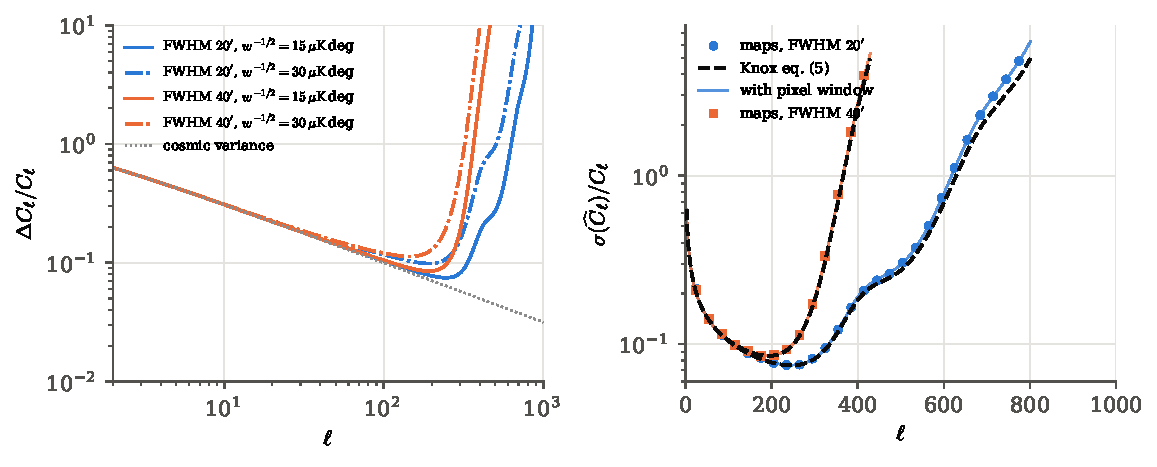
\includegraphics[width=12.5cm]{figures/ch08/knox_fig2.pdf}
\caption{Knox's Fig.~2, redone. Left: $\Delta\Cell/\Cell$ of \eqref{8a:eq:knox5} (his eq.~5) for his four experiments,
with our fiducial spectrum: the $20'$ beam (blue) beats the $40'$ beam (orange) at every $\ell$ for
both noise levels (solid and dash-dotted). Right: the two $w^{-1/2}=15\,\mu$K\,deg experiments
simulated with maps at $N_{\rm side}=512$. The simulated scatter (points) follows Knox's formula
(dashed) until the pixel window, which his formula leaves out, becomes visible; the formula with
the pixel window divided out (thin solid) follows the points everywhere.}
\label{8a:fig:knox}
\end{figure}

\paragraph{His formula, tested with maps.}
Knox never made a map. He drew each $C^{\rm est}_\ell$ directly from its $\chi^2_{2\ell+1}$
distribution \srcref{Knox1995}{p.~8}. A map contains things a formula can leave out, so we
simulated the two $w^{-1/2}=15\,\mu$K\,deg experiments as full maps. Script
\pyname{11_knox_reproduction.py} does five things for each experiment:
\begin{enumerate}
  \item draws a sky from the fiducial $\Cell$ and smooths it with the $20'$ or $40'$ beam;
  \item stores it in pixels at $N_{\rm side}=\EightAKnoxNside$, which applies the pixel window $p_\ell$;
  \item adds white noise of depth $w^{-1/2}=15\,\mu$K\,deg$\,=900\,\mu$K\,arcmin;
  \item computes $\Chat$ with \eqref{8a:eq:chat} up to $\ell=\EightAKnoxLmax$, dividing by the full
        $T_\ell^2=B_\ell^2p_\ell^2$;
  \item repeats this for $\EightAKnoxNsim$ skies (in $\EightAKnoxMinutes$ minutes), takes the standard
        deviation of $\Chat$ over the skies at each $\ell$, and divides it by two predictions:
        \eqref{8a:eq:var} with the pixel window included, and Knox's \eqref{8a:eq:knox4} as printed.
\end{enumerate}
The right panel of \cref{8a:fig:knox} shows the result, and \cref{8a:tab:literature} lists the
numbers. Against \eqref{8a:eq:var}, the simulated scatter averaged over $\ell$ is
$\EightAKnoxROursTwenty$ times the prediction for the $20'$ beam and $\EightAKnoxROursForty$ for the
$40'$ beam, where the Monte Carlo error is $\EightAKnoxMCerr\%$ per multipole. Against Knox's formula
as printed, the median ratio is $\EightAKnoxRKnoxTwenty$ for the $20'$ beam and
$\EightAKnoxRKnoxForty$ for the $40'$ beam, and for the $20'$ beam it climbs to
$\EightAKnoxRHiTwenty$ near $\ell=\EightAKnoxLgoodTwenty$.

\paragraph{Why his formula and the maps differ.}
The cause is the pixel window. Knox's footnote says that his formula ignores pixelisation, which
is harmless when the pixels are several times smaller than the beam. Our $6.9'$ pixels are three
times smaller than the $20'$ beam, yet by $\ell\approx800$ the pixel window has turned the signal
down by a further $p_\ell^2\approx0.8$. Dividing it out turns the noise on the sky,
$N_\ell/T_\ell^2$, up by $1/p_\ell^2\approx1.25$. Near $\ell=\EightAKnoxLgoodTwenty$ the noise term
dominates the bracket of \eqref{8a:eq:var}, so the error bar rises by about the same factor, which is
the $\EightAKnoxRHiTwenty$ the maps show. The $40'$ experiment loses its signal to the beam well
before the pixel window matters, so its ratio stays close to one. A formula can be correct for the
assumptions it states and still not describe a pixelised map.

\paragraph{His shortcut, and what it teaches about cost.}
Drawing $\EightAKnoxNsim$ sets of spectra directly from the shifted $\chi^2$ of
\eqref{8a:eq:shifted-chi2} takes $\EightAKnoxShortMs$\,ms, against minutes for the maps, and gives
the same scatter to a ratio of $\EightAKnoxShortRatio$. On the full sky with white noise the
map step adds nothing, because the distribution of $\Chat$ is known exactly. Maps become
necessary as soon as something breaks that distribution: a mask, inhomogeneous or correlated
noise, an asymmetric beam. The cheapest simulation that still contains the effect under study
is the right one, and that choice is what keeps a research pipeline on a laptop.

\subsection{Hivon et al.\ (2002): MASTER in the full-sky limit}
\label{8a:sec:lit-hivon}

\paragraph{Their question.}
By 2002 balloon experiments such as Boomerang had maps with hundreds of thousands of pixels, far
beyond the reach of the likelihood of \cref{8a:sec:why-not-ml}. The cheap alternative is the
\newterm{pseudo-spectrum} $\tilde C_\ell$: compute the spectrum of the observed map as if it were a
complete sky. But the map covers only a patch, has been filtered to remove slow detector drifts,
is blurred by the beam and contains noise, so on average $\tilde C_\ell$ is not $\Cell$: it is
biased, and power from neighbouring multipoles is mixed into it. Hivon et al.\ asked how to
correct this cheap estimator using nothing but simulations of the experiment, and how many
simulations that takes.

\paragraph{Their setup.}
Each thing the observation does to the sky gets one symbol, and it helps to meet them one at a
time.
\begin{itemize}
  \item \emph{The mask.} Only a patch of sky is kept. Cutting the sky mixes multipoles, and the
        mixing is described by a \newterm{mode-coupling matrix} $M_{\ell\ell'}$: how much of the true
        power at $\ell'$ ends up in the pseudo-spectrum at $\ell$.
  \item \emph{The filter.} The time-ordered data are high-pass filtered before the map is made,
        which removes large-scale power by a factor $F_\ell$ at each $\ell$, measured from noise-free
        simulations.
  \item \emph{The beam and the pixel.} Their window $B_\ell$ is the beam times the pixel window, our
        $T_\ell$ of \eqref{8a:eq:transfer}.
  \item \emph{The noise.} Its average power in the pseudo-spectrum, $\langle\tilde N_\ell\rangle$, is
        measured from noise-only simulations.
\end{itemize}
Their test simulated the Boomerang long-duration flight (\cref{8a:tab:hivon-setup})
\srcref{Hivon}{§4.1}.

\begin{table}[htbp]
\centering
\small
\renewcommand{\arraystretch}{1.2}
\begin{tabular}{@{}>{\raggedright\arraybackslash}p{3.0cm}>{\raggedright\arraybackslash}p{4.6cm}>{\raggedright\arraybackslash}p{4.4cm}@{}}
\hline
 & Hivon et al.\ (2002) & ours \\
\hline
beam FWHM & $10'$ & $30'$ \\
map resolution & $N_{\rm side}=512$ & $N_{\rm side}=256$ \\
noise & measured spectrum of one detector, with its $1/f$ rise and scan lines & white, uniform \\
filter & sharp high-pass & none \\
sky region & ellipse, $\fsky=1.82\%$ & full sky \\
simulations & $450$ noise-only, $250$ noise-free, $1350$ signal plus noise & $\EightANsim$ signal plus noise \\
\hline
\end{tabular}
\caption{The MASTER test and ours.}
\label{8a:tab:hivon-setup}
\end{table}

\paragraph{Their notation, and ours.}
Their pseudo-spectrum $\tilde C_\ell$ of the observed map is our $\widehat C^{\,\rm obs}_\ell$ of
\eqref{8a:eq:cobs} when the sky is complete; their $B_\ell$ is our $T_\ell=B_\ell p_\ell$; their
$\langle\tilde N_\ell\rangle$ is our average noise power $\bar N_\ell$ of \eqref{8a:eq:nbar}; their
$C_b$ and $N_b$ are our spectrum and noise power averaged over a bin $b$ of $\Delta\ell$ multipoles;
their $F_\ell$ and $M_{\ell\ell'}$ have no counterpart on our full, unfiltered sky.

\paragraph{Their master equation.}
Why does the average pseudo-spectrum take the form of a matrix acting on $\Cell$? Three moves give
it.
\begin{enumerate}
  \item The observed sky is the true sky times the mask, $s(\hat{\bm n})M(\hat{\bm n})$, with $M=1$
        on the patch and $0$ elsewhere.
  \item In harmonic space a product becomes a sum: each coefficient of the masked sky is a sum of
        the true coefficients $a_{\ell'm'}$ over all $\ell'$, weighted by the harmonics of the mask
        itself (\cref{8a:sec:knox}). So one $\ell$ of the pseudo-spectrum receives power from
        several $\ell'$.
  \item Square the coefficients and average over skies. Different true coefficients are
        uncorrelated, so only the diagonal terms $\langle|a_{\ell'm'}|^2\rangle=C_{\ell'}$ survive. What
        remains is a fixed matrix, set by the mask alone, acting on the vector of $C_{\ell'}$:
        $M_{\ell\ell'}$.
\end{enumerate}
The filter and the beam act on the sky before the mask, so they multiply each $C_{\ell'}$ by
$F_{\ell'}B_{\ell'}^2$, and the noise adds its own average power. This is Hivon's eq.~(15), and
the form of $M_{\ell\ell'}$ is derived for the masked sky in \cref{8b:sec:kernel}. With no mask
($M=1$ everywhere) and no filter,
\begin{equation}
  \langle\tilde C_\ell\rangle
  \eqby{1}\sum_{\ell'}M_{\ell\ell'}F_{\ell'}B_{\ell'}^2\langle C_{\ell'}\rangle+\langle\tilde N_\ell\rangle
  \eqby{2}T_\ell^2\,\Cell+\bar N_\ell ,
  \nonumber
\end{equation}
\begin{explain}
  \item Hivon's eq.~(15).
  \item With $M=1$ the masked sky is the sky, no multipoles are mixed and $M_{\ell\ell'}=\delta_{\ell\ell'}$;
        no filter means $F_\ell=1$; $B_\ell=T_\ell$ and $\langle\tilde N_\ell\rangle=\bar N_\ell$ of \eqref{8a:eq:nbar}.
\end{explain}
which is our \eqref{8a:eq:cobs-mean}: what remains is the beam, the pixel window and the noise. Every
statement of the paper about those three can therefore be tested on our full-sky
simulations; the statements about the mask are taken up with the masked sky.

\paragraph{Noise-bias removal.}
Hivon et al.\ found the recovered spectrum unbiased both where the signal dominates and
where the signal-to-noise is very low \srcref{Hivon}{§4.2, Fig.~5}. Our debiased estimator passes
the corresponding test with $\chi^2=\EightAChiAuto$ for $\EightANbins$ bins
(\cref{8a:sec:res-bias}).

\paragraph{The analytic error bar.}
Their rule of thumb \srcref{Hivon}{(16)--(17)} gives the error of a bin of $\Delta\ell$ multipoles as
$(C_b+N_b/T_b^2)\sqrt{2/\nu_b}$ with $\nu_b=(2\ell_b+1)\Delta\ell\fsky w_2^2/w_4$, and they found
their simulated errors ``almost identical'' to it. The rule follows from \eqref{8a:eq:var} in two steps. The binned estimate
is the plain average $\widehat C_b=\Delta\ell^{-1}\sum_{\ell\in b}\Chat$ over the $\Delta\ell$
multipoles of bin $b$, centred on $\ell_b$. On the full sky,
\begin{align}
  \Var\bigl(\widehat C_b\bigr)
  &\eqby{1}\frac{1}{\Delta\ell^2}\sum_{\ell\in b}\Var\bigl(\Chat\bigr)
   \eqby{2}\frac{1}{\Delta\ell^2}\sum_{\ell\in b}\frac{2}{2\ell+1}\Bigl(\Cell+\frac{N_\ell}{T_\ell^2}\Bigr)^2
   \nonumber\\
  &\relby{3}{\approx}\frac{2}{(2\ell_b+1)\,\Delta\ell}\Bigl(C_b+\frac{N_b}{T_b^2}\Bigr)^2 .
  \label{8a:eq:hivon16}
\end{align}
\begin{explain}
  \item Different multipoles of a full sky are independent, so the variances of the $\Delta\ell$
        terms add, and the factor $1/\Delta\ell$ comes out squared.
  \item The single-multipole variance \eqref{8a:eq:var}.
  \item If $\Cell$, $N_\ell/T_\ell^2$ and $2\ell+1$ change little across the bin, the $\Delta\ell$
        terms are all close to the one at $\ell_b$, and their sum is $\Delta\ell$ times it.
\end{explain}
The square root of \eqref{8a:eq:hivon16} is $(C_b+N_b/T_b^2)\sqrt{2/\nu_b}$ with
$\nu_b=(2\ell_b+1)\Delta\ell$, the number of modes in the bin. On part of the sky the mode count
of \cref{8a:sec:knox} multiplies $\nu_b$ by $\fsky$, and by $w_2^2/w_4$ for a weighted mask,
which gives their eqs.~(16)--(17). The quantity compared is therefore our simulated standard
deviation of $\widehat C_b$ divided by the square root of \eqref{8a:eq:hivon16} with
$\fsky=1$, and, separately, divided by the square root of line~2, which makes no assumption
about the bin. On the full sky, in bins of $\Delta\ell=50$,
our simulated error divided by the rule lies between $\EightAHivRsixteenMin$ and
$\EightAHivRsixteenMax$ in the bins above $\ell=63$, with a Monte Carlo error of
$\EightAHivRsixteenErr\%$. The first bin, $\ell=13$--$62$, is the exception, with a ratio of
$\EightAHivRfirst$. The rule evaluates the spectrum at the bin average, but $\Cell$ falls by a
factor of about twenty across that bin, and the variance of a bin average,
$\sum_\ell\Var(\Chat)/\Delta\ell^2$, is dominated by the largest $\Cell$ in it. The exact
expression, line~2 of \eqref{8a:eq:hivon16}, gives ratios between $\EightAHivRexactMin$ and
$\EightAHivRexactMax$ in every bin. The rule fails exactly at its step~3: it needs a spectrum that
is nearly constant across the bin.

\paragraph{How fast the calibrations converge.}
MASTER estimates three things by simulation: the transfer function, the noise power, and the
error bars. Each estimate comes from a finite number $N$ of simulations, so each carries a
Monte Carlo error of its own. The question is: \emph{how large is that error, and how does it
shrink with $N$?} Hivon et al.\ give the answers as their eqs.~(38)--(42) \srcref{Hivon}{(38)--(42)}.
We derive them from the mode count of \eqref{8a:eq:hivon16}.

\emph{The transfer function and the noise power.} Each is an average over the $N$ simulations of
one binned spectrum, call it $X_b$: the noise-free spectrum divided by the input spectrum for the
transfer function, the noise-only spectrum for the noise power. In one simulation, $X_b$ is built
from $\nu_b=(2\ell_b+1)\Delta\ell$ independent modes, so by \eqref{8a:eq:hivon16} it scatters by
$\sigma(X_b)=\sqrt{2/\nu_b}\,\langle X_b\rangle$. Averaging $N$ independent simulations reduces
that scatter by $\sqrt N$.

\emph{The error bar.} It is the standard deviation $s$ of $\widehat C_b$ over the $N$
simulations. With many modes in a bin, $\widehat C_b$ is close to Gaussian, and then
$(N-1)s^2/\sigma^2$ is a $\chi^2_{N-1}$ variable (\cref{ch:03}), whose variance we know.

Then
\begin{align}
  \frac{\delta\bar X_b}{\langle X_b\rangle}
  &\eqby{1}\frac{\sigma(X_b)/\sqrt N}{\langle X_b\rangle}
   \eqby{2}\sqrt{\frac{2}{(2\ell_b+1)\,\Delta\ell\,N}} ,
  \label{8a:eq:conv-transfer}\\
  \frac{\delta s}{s}
  &\eqby{3}\frac12\,\frac{\delta(s^2)}{\sigma^2}
   \eqby{4}\frac12\sqrt{\frac{2}{N-1}}
   =\frac{1}{\sqrt{2(N-1)}} .
  \label{8a:eq:conv-sd}
\end{align}
\begin{explain}
  \item The average of $N$ independent copies has $1/N$ times the variance of one.
  \item $\sigma(X_b)=\sqrt{2/\nu_b}\,\langle X_b\rangle$ with $\nu_b=(2\ell_b+1)\Delta\ell$; on part of
        the sky $\nu_b$ carries the factor $\fsky$, which gives \srcref{Hivon}{(19), (38)--(39)}.
  \item Error propagation for $s=\sqrt{s^2}$: $\delta s=\delta(s^2)/(2s)$, and $s\approx\sigma$.
  \item $s^2=\sigma^2\chi^2_{N-1}/(N-1)$ and $\Var(\chi^2_{N-1})=2(N-1)$, so
        $\delta(s^2)=\sigma^2\sqrt{2/(N-1)}$.
\end{explain}
Third, the error that an $N$-simulation noise estimate puts on $\Chat$, relative to its
statistical error, is $N_\ell/(T_\ell^2\Cell+N_\ell)\cdot N^{-1/2}$, derived in
\eqref{8a:eq:nsim-noise}. What is compared is the scatter of each Monte Carlo estimate between
disjoint groups of $N$ of our skies, divided by \eqref{8a:eq:conv-transfer},
\eqref{8a:eq:conv-sd} or \eqref{8a:eq:nsim-noise}. Script \pyname{12_hivon_convergence.py} measures all four by splitting
our $\EightANsim$ skies into disjoint groups of $N=25$ to $400$ (\cref{8a:fig:hivon}). At $N=100$ the
measured scatter divided by our formula is $\EightAHivFratio$ for the transfer function,
$\EightAHivNratio$ for the noise power, $\EightAHivSDratio$ for the error bar and
$\EightAHivMethratio$ for the noise-induced error, each $\pm\EightAHivFratioErr$.

The published coefficients are larger, and most of the difference can be traced. Take the
transfer function and the noise power at $\ell\approx400$, $\Delta\ell=50$ and $N=100$. Our full-sky
formula \eqref{8a:eq:conv-transfer} gives $\EightAHivFfull\%$; Hivon's numbers are $0.6$--$0.9\%$.
Two causes act through the mode count $\nu_b$, and the error goes as $1/\sqrt{\nu_b}$.
\begin{itemize}
  \item \emph{The sky fraction.} Their region is $1.82\%$ of the sky, so $\nu_b$ carries the factor
        $\fsky=0.0182$ and the error rises by $1/\sqrt{0.0182}=7.4$: from $\EightAHivFfull\%$ to
        $\EightAHivFresc\%$. After this step their numbers are still $0.6/\EightAHivFresc=1.13$ to
        $0.9/\EightAHivFresc=1.70$ times ours.
  \item \emph{The weighting.} They weighted their region with a cosine-apodised window, for which
        $w_2^2/w_4=0.5$. In \eqref{8a:eq:knox-fsky} this factor multiplies $\fsky$, so it halves
        $\nu_b$ and raises the error by $\sqrt2=1.41$: from $\EightAHivFresc\%$ to $0.75\%$.
\end{itemize}
Their range now sits on either side of ours: $0.6/0.75=0.8$ and $0.9/0.75=1.2$. What is left, a
factor between $0.8$ and $1.2$, depends on details of their region that our full-sky model does not
contain, such as the uneven number of observations across the patch and the correlated noise of
their detector. We do not reproduce it, and with a full sky we cannot.
For the error bar, their ``$0.1\sqrt{100/N}$'' is a rounded upper value of
$1/\sqrt{2(N-1)}=\EightAHivSDth\%$ at $N=100$, which our groups reproduce. For the noise-induced
error, their $0.1\sqrt{100/N}$ is exactly $1/\sqrt N$, our \eqref{8a:eq:nsim-noise} in the deeply
noise-dominated limit; in our last bin the noise is $\EightAHivNDfrac$ of the power, so the formula
gives $\EightAHivMethth\%$ and the groups give $\EightAHivMethmc\%$.

\begin{figure}[htbp]
\centering
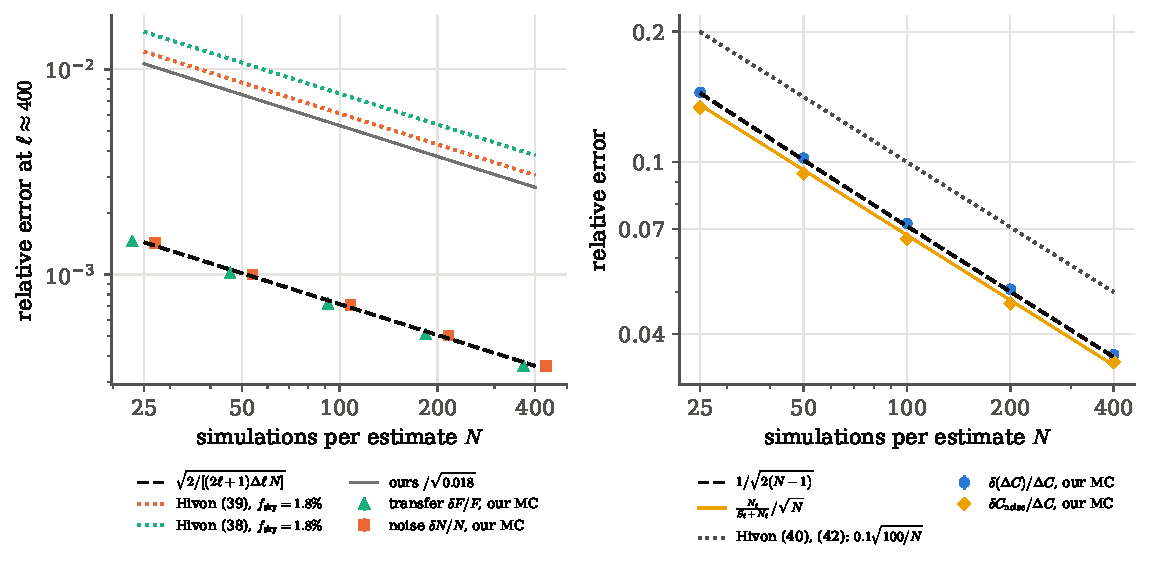
\includegraphics[width=12.5cm]{figures/ch08/hivon_convergence.pdf}
\caption{Hivon et al.'s convergence laws against our simulations. Left: the relative Monte Carlo
error of the transfer function (green) and of the noise power (orange) at $\ell\approx400$ in
bins of $50$, from disjoint groups of $N$ skies, on the full-sky law (dashed). Hivon's published
laws for $1.8\%$ of the sky (dotted) lie above it by about $1/\sqrt{\fsky}$ (grey). Right: the
relative error of an estimated error bar (blue) and the error a noise estimate adds to $\Chat$
(yellow), against $1/\sqrt{2(N-1)}$ (dashed), its noise-weighted version (yellow line) and
Hivon's $0.1\sqrt{100/N}$ (dotted).}
\label{8a:fig:hivon}
\end{figure}

\paragraph{The shape of the distribution.}
Hivon et al.\ showed that at small numbers of modes a $\chi^2_\nu$ with no free parameter
describes the simulated estimates far better than a Gaussian of the same mean and width
\srcref{Hivon}{§4.2, Fig.~6}. On the full sky the number of modes is small only at the lowest
multipoles. At $\ell=3$, $\nu=7$, the shifted $\chi^2$ passes the Kolmogorov--Smirnov test with
$p=\EightAHivKSchi$ and the Gaussian fails with $p=\EightAHivKSgauss$
(\cref{8a:sec:res-shape}). Their small $\fsky$ brought the same effect up to $\ell\sim100$; that
version needs the mask.

\paragraph{What reproducing it taught us.}
On the full sky every claim MASTER makes about the beam, the pixel window and the noise is checked
by our machine, and the one failure we found, in the first bin, shows that the binned rule of
thumb needs a spectrum that is flat across the bin. The claims that depend on the mask are not
reproduced here.

\begin{table}[htbp]
\centering
\small
\renewcommand{\arraystretch}{1.25}
\begin{tabular}{@{}>{\raggedright\arraybackslash}p{3.6cm}>{\raggedright\arraybackslash}p{2.4cm}>{\raggedright\arraybackslash}p{2.6cm}>{\raggedright\arraybackslash}p{3.6cm}@{}}
\hline
quantity & published & ours & why they differ \\
\hline
\multicolumn{4}{@{}l}{\emph{Knox (1995)}}\\
$w^{-1/2}$ for $22\,\mu$K in $20'$ pixels & $7.5\,\mu$K\,deg & $\EightAKnoxWinv\,\mu$K\,deg & his rounding \\
sky rms through a $20'$ beam & $92.5\,\mu$K & $\EightAKnoxRms\,\mu$K & sCDM vs Planck 2018 \\
signal-to-noise per pixel & $\simeq4$ & $\EightAKnoxSnrPix$ & same \\
error formula, eq.~(4) & exact & maps: $\EightAKnoxROursTwenty$ & with $p_\ell$ divided out \\
\quad as printed, $20'$ beam & --- & median $\EightAKnoxRKnoxTwenty$ & no pixel window in eq.~(4) \\
smaller beam wins at fixed $w$ & every $\ell$ & every $\ell\le1000$ & --- \\
$N$ for $\sigma$ to $10\%$ & ``100 suffice'' & $\EightANTenPct$ ($7.1\%$ at $100$) & --- \\
\hline
\multicolumn{4}{@{}l}{\emph{Hivon et al.\ (2002), full-sky limit}}\\
bias after noise removal & none (Fig.~5) & $\chi^2=\EightAChiAuto/\EightANbins$ & --- \\
MC error / rule (16) & ``almost identical'' & $\EightAHivRsixteenMin$--$\EightAHivRsixteenMax$ & first bin $\EightAHivRfirst$: $\Cell$ not flat \\
$\delta F/F$, $\delta N/N$ at $N=100$ & $0.6$--$0.9\%$ & $\EightAHivFmc\%$ & $\fsky=1.8\%$; ours $/\sqrt{\fsky}$: $\EightAHivFresc\%$ \\
$\delta(\Delta C)/\Delta C$ at $N=100$ & $\approx10\%$ & $\EightAHivSDmc\%$ & their value is rounded up \\
noise error / stat.\ error & $10\%$ & $\EightAHivMethmc\%$ & our bin only $\EightAHivNDfrac$ noise \\
$\chi^2$ vs Gaussian, few modes & $\chi^2$ wins & KS $p$: $\EightAHivKSchi$ vs $\EightAHivKSgauss$ & full sky: only at low $\ell$ \\
simulations & $450+250+1350$ & $\EightANsim$ & ours are cheaper, simpler \\
\hline
\end{tabular}
\caption{Published numbers and the same quantities from our code. ``Maps'' is the simulated
scatter divided by the formula, averaged over $\ell$.}
\label{8a:tab:literature}
\end{table}

\subsection{Planck's pivot: why \texorpdfstring{$A_s$ and $n_s$ are quoted at $k_*=0.05\,{\rm Mpc}^{-1}$}{A\_s and n\_s are quoted at k = 0.05/Mpc}}
\label{8a:sec:lit-pivot}

Planck reports two numbers for the primordial fluctuations: their amplitude,
$\ln(10^{10}A_s)=3.044\pm0.014$, and their tilt, $n_s=0.9649\pm0.0042$ (\cref{ch:T1}). The amplitude
is the one ``which we define at the pivot scale $k_0=0.05\,{\rm Mpc}^{-1}$'' \cite{Planck2018VI}.
WMAP quoted its amplitude at a different scale, $k=0.002\,{\rm Mpc}^{-1}$, and Planck still quotes
the tensor-to-scalar ratio there, $r_{0.002}<0.10$ \cite{Planck2018VI}. Why does an amplitude need
a scale attached to it at all, and why this one?

\paragraph{The spectrum is a straight line.}
The primordial spectrum is a power law,
\begin{equation}
  \mathcal P(k)=A_s\Bigl(\frac{k}{k_0}\Bigr)^{n_s-1},
  \label{8a:eq:pivot-pk}
\end{equation}
so $\ln\mathcal P=\ln A_s+(n_s-1)\ln(k/k_0)$. Plotted as $\ln\mathcal P$ against $\ln k$ it is a
straight line. Its slope is $n_s-1$. Its height at the point $k=k_0$ is $\ln A_s$. That point,
the \newterm{pivot}, is our choice: we may describe the same line by its height at any $k$ we
like. The slope stays the same whichever point we choose. The height changes, and so does
something less obvious: how strongly the measured height and the measured slope are correlated.

Think of fitting a straight line through points. If we report the height of the line far to the
left of the data, any error in the slope swings that height up or down, so height and slope come
out strongly correlated. If we report the height in the middle of the data, a small change of
slope just pivots the line about that point, and the height hardly moves: the two errors are
independent. The pivot scale is the same idea. The question, in words: \emph{at which $k$ do the
measured amplitude and the measured tilt become uncorrelated, and where does that $k$ sit?}

\paragraph{Step 1: what moving the pivot does.}
Call $A(k_0)$ the amplitude quoted at $k_0$, and write $n$ for $n_s$. The same spectrum,
evaluated at another point $k_1$, has height $A(k_1)=A(k_0)\,(k_1/k_0)^{n-1}$; this is just
\eqref{8a:eq:pivot-pk} at $k=k_1$. Write $L=\ln(k_1/k_0)$ for the distance between the two
points in $\ln k$. It is a fixed number, not a measured one. Then
\begin{align}
  \ln A(k_1)&\eqby{1}\ln A(k_0)+(n-1)\,L ,
  \label{8a:eq:pivot-shift}\\
  \Cov\bigl(\ln A(k_1),n\bigr)
  &\eqby{2}\Cov\bigl(\ln A(k_0),n\bigr)+L\,\Var(n),
  \nonumber\\
  \Var\bigl(\ln A(k_1)\bigr)
  &\eqby{3}\Var\bigl(\ln A(k_0)\bigr)+2L\,\Cov\bigl(\ln A(k_0),n\bigr)+L^2\,\Var(n).
  \nonumber
\end{align}
\begin{explain}
  \item Take the logarithm of $A(k_1)=A(k_0)(k_1/k_0)^{n-1}$.
  \item Take the covariance of both sides of line~1 with $n$. A covariance splits over a sum. The
        constant $-L$ hidden in $(n-1)L$ does not fluctuate, so it drops out, and the covariance of
        $n$ with itself is its variance.
  \item The variance of a sum $X+LY$ is $\Var X+2L\Cov(X,Y)+L^2\Var Y$; here $X=\ln A(k_0)$ and $Y=n$.
\end{explain}
Line~2 says that moving the pivot by $L$ shifts the covariance by $L\,\Var(n)$. So there is
exactly one pivot at which the covariance is zero. Setting line~2 to zero and solving for $L$
gives the \newterm{decorrelation pivot}:
\begin{equation}
  L_{\rm dec}=-\frac{\Cov\bigl(\ln A(k_0),n\bigr)}{\Var(n)},
  \qquad
  k_{\rm dec}=k_0\exp\Bigl[-\frac{\Cov\bigl(\ln A(k_0),n\bigr)}{\Var(n)}\Bigr].
  \label{8a:eq:kdec}
\end{equation}
Line~3 gives a bonus. Its derivative with respect to $L$ is $2\Cov+2L\Var(n)$, which vanishes at
the same $L_{\rm dec}$. So the pivot that makes the two numbers independent is also the pivot at
which the amplitude has its smallest error. All \eqref{8a:eq:kdec} needs is the covariance of the
two numbers at one pivot, however it was obtained: from a Fisher matrix, a Markov chain or a fit.

\paragraph{Step 2: from wavenumber to multipole.}
The data are multipoles, the pivot is a wavenumber, so first we need to know which multipoles
see which wavenumbers.
The CMB is a picture of the last-scattering sphere, at comoving distance $D_*$ from us. A wave of
wavenumber $k$ on that sphere has wavelength $2\pi/k$. Seen from a distance $D_*$, that length
spans an angle of $2\pi/(kD_*)$ radians. A spherical harmonic of degree $\ell$ has an angular
wavelength of $2\pi/\ell$. Matching the two, $\ell\approx kD_*$. CAMB gives
$D_*=\EightAPivDstar$\,Gpc for the fiducial model (see the cosmology notes). So the Planck pivot
$0.05\,{\rm Mpc}^{-1}$ sits at $\ell\approx\EightAPivLfive$, and the WMAP pivot
$0.002\,{\rm Mpc}^{-1}$ at $\ell\approx\EightAPivLtwo$. The match is approximate: a wave whose crests
are not perpendicular to our line of sight looks longer on the sky, so one $k$ also feeds every
$\ell$ below $kD_*$. Turned around: multipole $\ell$ receives power from a range of wavenumbers,
through a kernel $G_\ell(k)$ that peaks near $k_\ell\equiv\ell/D_*$ and has a tail towards larger $k$.
The temperature spectrum is linear in the primordial one,
\begin{equation}
  \Cell=\int G_\ell(k)\,\mathcal P(k)\,\dd\ln k ,
  \label{8a:eq:pivot-kernel}
\end{equation}
with $G_\ell\ge0$ fixed by the physics between the early universe and last scattering, which CAMB
computes.

\paragraph{Step 3: how much each multipole knows.}
To use \eqref{8a:eq:kdec} we need that covariance for a temperature measurement, and the Fisher
matrix of \cref{ch:10} gives it. We already have the Fisher information of one $\Cell$,
\eqref{8a:eq:fisher-cl}. We need it for the parameters $\theta_i$ that the spectrum depends on.
Two facts make this a short step. On the full sky different multipoles are independent, so their
informations add. And the parameters reach the data only through $\Cell$, so the chain rule
converts information on $\Cell$ into information on $\theta_i$:
\begin{align}
  F_{ij}\equiv\Bigl\langle\frac{\partial^2(-\ln\Like)}{\partial\theta_i\partial\theta_j}\Bigr\rangle
  &\eqby{1}\sum_\ell\Bigl\langle\frac{\partial^2(-\ln\Like_\ell)}{\partial\Cell^2}\Bigr\rangle
     \frac{\partial\Cell}{\partial\theta_i}\frac{\partial\Cell}{\partial\theta_j}
   \eqby{2}\sum_\ell\frac{(2\ell+1)\fsky}{2\,(\Cell+N_\ell/T_\ell^2)^2}\,
     \frac{\partial\Cell}{\partial\theta_i}\frac{\partial\Cell}{\partial\theta_j}.
  \label{8a:eq:fisher-params}
\end{align}
\begin{explain}
  \item Write $\ln\Like=\sum_\ell\ln\Like_\ell$ and differentiate twice with the chain rule. One
        term contains $\partial^2\Cell/\partial\theta_i\partial\theta_j$, but it is multiplied by
        the average slope of $-\ln\Like_\ell$, which is zero at the true parameters (\cref{ch:03}).
  \item The information on one $\Cell$ is \eqref{8a:eq:fisher-cl}. On part of the sky there are
        only $(2\ell+1)\fsky$ modes instead of $2\ell+1$ (\cref{8a:sec:knox}).
\end{explain}

Now the two parameters. How does $\Cell$ change when each of them is nudged? Differentiate
\eqref{8a:eq:pivot-kernel} under the integral; the kernel does not depend on $A$ or $n$.
The amplitude multiplies $\mathcal P(k)$ at every $k$, so $\partial\mathcal P/\partial\ln A=\mathcal P$.
The tilt enters through $\ln\mathcal P=\ln A+(n-1)\ln(k/k_0)$, so $\partial\mathcal P/\partial n=\mathcal P\ln(k/k_0)$:
raising $n$ raises the spectrum more at large $k$ and lowers it at $k<k_0$. Then
\begin{align}
  \frac{\partial\Cell}{\partial\ln A}
  &\eqby{1}\int G_\ell\,\mathcal P\,\dd\ln k=\Cell ,
  \nonumber\\
  \frac{\partial\Cell}{\partial n}
  &\eqby{2}\int G_\ell\,\mathcal P\,\ln\frac{k}{k_0}\,\dd\ln k
   \eqby{3}\Cell\,\Bigl\langle\ln\frac{k}{k_0}\Bigr\rangle_\ell
   \relby{4}{\approx}\Cell\,g_\ell ,\qquad g_\ell\equiv\ln\frac{k_\ell}{k_0}.
  \nonumber
\end{align}
\begin{explain}
  \item $\partial\mathcal P/\partial\ln A=\mathcal P$, and the integral is \eqref{8a:eq:pivot-kernel}.
  \item $\partial\mathcal P/\partial n=\mathcal P\ln(k/k_0)$.
  \item Divide and multiply by $\Cell$: $\langle\cdot\rangle_\ell$ is the average over $\ln k$ with
        weight $G_\ell\mathcal P/\Cell$, which integrates to one.
  \item Replace the kernel by a spike at its peak $k_\ell=\ell/D_*$ (Step~2). The tail of the kernel
        towards larger $k$ makes this a shortcut, not an exact step; the script below keeps the
        full kernel.
\end{explain}
So $g_\ell$ is the distance of multipole $\ell$ from the pivot in $\ln k$. Put the two derivatives
into \eqref{8a:eq:fisher-params}. Every term carries the same factor, which we name the
\newterm{information weight} of multipole $\ell$,
\[
  \mathcal I_\ell\equiv\frac{(2\ell+1)\fsky}{2}\Bigl[\frac{\Cell}{\Cell+N_\ell/T_\ell^2}\Bigr]^2 ,
\]
the information that multipole $\ell$ carries about $\ln A$: its number of modes, cut down where
the noise on the sky $N_\ell/T_\ell^2$ exceeds the signal. Since
$\frac{(2\ell+1)\fsky}{2(\Cell+N_\ell/T_\ell^2)^2}=\mathcal I_\ell/\Cell^2$, the three entries are
\[
  F_{AA}=\sum_\ell\frac{\mathcal I_\ell}{\Cell^2}\,\Cell^2=\sum_\ell\mathcal I_\ell,\qquad
  F_{An}=\sum_\ell\frac{\mathcal I_\ell}{\Cell^2}\,\Cell\cdot\Cell g_\ell=\sum_\ell\mathcal I_\ell\,g_\ell,\qquad
  F_{nn}=\sum_\ell\mathcal I_\ell\,g_\ell^2,
\]
so that
\[
  F=\begin{pmatrix}\sum_\ell \mathcal I_\ell & \sum_\ell \mathcal I_\ell g_\ell\\[2pt] \sum_\ell \mathcal I_\ell g_\ell & \sum_\ell \mathcal I_\ell g_\ell^2\end{pmatrix}.
\]
Its inverse is the covariance. For a $2\times2$ matrix
$\bigl(\begin{smallmatrix}a&b\\b&c\end{smallmatrix}\bigr)$ the inverse is
$\bigl(\begin{smallmatrix}c&-b\\-b&a\end{smallmatrix}\bigr)/\det F$, so the covariance of the two
numbers is $-b/\det F$ and the variance of $n$ is $a/\det F$. Put them into \eqref{8a:eq:kdec}:
\[
  \ln\frac{k_{\rm dec}}{k_0}=-\frac{\Cov(\ln A,n)}{\Var(n)}
  \eqby{1}\frac{\sum_\ell \mathcal I_\ell g_\ell}{\sum_\ell \mathcal I_\ell}
  \eqby{2}\frac{\sum_\ell \mathcal I_\ell\,\ln(k_\ell/k_0)}{\sum_\ell \mathcal I_\ell},
\]
\begin{explain}
  \item $-(-b/\det F)/(a/\det F)=b/a$; the determinant cancels.
  \item Write out $g_\ell$.
\end{explain}
Adding $\ln k_0$ to both sides, $\ln k_{\rm dec}=\sum_\ell \mathcal I_\ell\ln k_\ell/\sum_\ell \mathcal I_\ell$. In words:
\emph{the decorrelation pivot is the average of $\ln k$ over the scales the data measure, each
scale counted with the weight of what it knows.} That is the straight-line picture made exact:
the height and the slope are independent when the height is quoted in the middle of the data,
and ``middle'' means the weighted middle. The sky fraction multiplies every $\mathcal I_\ell$, so it
cancels: observing less sky widens the errors but does not move $k_{\rm dec}$.

\paragraph{Step 4: the numbers.}
Script \pyname{14_pivot.py} does the calculation without the spike shortcut, for the Planck-like
experiment of \cref{8a:tab:pivot-setup}. It computes the temperature spectrum with CAMB; finds the
derivatives of $\Cell$ with respect to $\ln A$ and $n$ by nudging each up and down, at both pivots;
builds the Fisher matrix \eqref{8a:eq:fisher-params}; inverts it to get the covariance; and puts
that covariance into \eqref{8a:eq:kdec} to get $k_{\rm dec}$.

\begin{table}[htbp]
\centering
\small
\renewcommand{\arraystretch}{1.2}
\begin{tabular}{@{}>{\raggedright\arraybackslash}p{3.4cm}>{\raggedright\arraybackslash}p{8.2cm}@{}}
\hline
beam FWHM & $7'$ \\
white-noise depth & $33\,\mu$K\,arcmin \\
sky fraction & $\fsky=0.6$ \\
multipoles & $2\le\ell\le2500$, temperature only \\
free parameters & $\ln A$ and $n$; then all six $\Lambda$CDM parameters, with a Gaussian prior of width
                  $0.0073$ on $\tau$ standing in for the large-angle polarisation that fixes it \\
\hline
\end{tabular}
\caption{The idealised Planck-like experiment of the pivot calculation.}
\label{8a:tab:pivot-setup}
\end{table}

\begin{table}[htbp]
\centering
\small
\renewcommand{\arraystretch}{1.25}
\begin{tabular}{@{}>{\raggedright\arraybackslash}p{3.3cm}>{\raggedright\arraybackslash}p{1.9cm}>{\raggedright\arraybackslash}p{1.9cm}>{\raggedright\arraybackslash}p{5.0cm}@{}}
\hline
quantity & at $0.05\,{\rm Mpc}^{-1}$ & at $0.002\,{\rm Mpc}^{-1}$ & reason \\
\hline
correlation of $\ln A$ and $n$ & $\EightAPivRhoFive$ & $\EightAPivRhoTwo$ & $0.002$ lies far from the weighted middle of the data \\
\quad moved from $0.05$ by \eqref{8a:eq:pivot-shift} & --- & $\EightAPivRhoTwoTrans$ & the shift is exact \\
$k_{\rm dec}$ [Mpc$^{-1}$] & $\EightAPivKdec$ & $\EightAPivKdecFromTwo$ & a property of the data, not of the pivot \\
$\sigma(\ln A)$ & $\EightAPivSigAFive$ & $\EightAPivSigATwo$ & the $L^2\Var(n)$ term of line~3 \\
correlation, six parameters free & $\EightAPivRhoFiveMarg$ & $\EightAPivRhoTwoMarg$ & a common amplitude error from $\tau$ \\
\hline
\end{tabular}
\caption{The pivot calculation at the two pivots.}
\label{8a:tab:pivot-results}
\end{table}

\Cref{8a:tab:pivot-results} collects the results, and \cref{8a:fig:pivot} shows the correlation for
every pivot together with the weights $\mathcal I_\ell$. Each difference has a cause that the steps
above can size.

\emph{The correlation.} With only $\ln A$ and $n$ free, $k_{\rm dec}=\EightAPivKdec\,{\rm Mpc}^{-1}$,
that is $\ell_{\rm dec}\approx\EightAPivLdec$. The Planck pivot is at $\ell\approx\EightAPivLfive$, not
far below it, and the correlation there is moderate. The WMAP pivot is at $\ell\approx\EightAPivLtwo$,
far to the left of almost all the information, and there the two numbers are almost perfectly
anti-correlated: the straight-line picture of the height read off far from the data.

\emph{The check of Step~1.} Computing the Fisher matrix directly at $0.002\,{\rm Mpc}^{-1}$ and moving
the covariance there from $0.05\,{\rm Mpc}^{-1}$ with \eqref{8a:eq:pivot-shift} give the same
correlation, and both pivots give the same $k_{\rm dec}$: the decorrelation scale belongs to the data.
The spike shortcut of Step~3, the $\mathcal I_\ell$-weighted average of $\ln\ell$, gives
$\ell\approx\EightAPivLdecApprox$. It falls short of the exact $\EightAPivLdec$ because the kernel's
tail towards larger $k$ makes each multipole see slightly larger $k$ than $\ell/D_*$.

\emph{The amplitude error.} Moving from $0.05$ to $0.002\,{\rm Mpc}^{-1}$ is a step
$L=\ln(0.002/0.05)=-3.22$. Line~3 of \eqref{8a:eq:pivot-shift} then gives
$\Var(\ln A)$ at $0.002$ as $0.0017^2+2L\Cov+L^2\,\Var(n)$. With
$\sigma(n)=\EightAPivSigNsFive$ and the correlation $\EightAPivRhoFive$, the three terms are
$0.29$, $2.0$ and $6.5$ in units of $10^{-5}$; the square root of their sum is $0.0094$, the
$\EightAPivSigATwo$ of the table. The $L^2\Var(n)$ term carries three quarters of it: quoted far
from the data, the height inherits the uncertainty of the slope, magnified by the distance.

\emph{Marginalising.} With all six $\Lambda$CDM parameters free, the covariance of $\ln A$ and $n$ is
read from the inverse of the full six-by-six Fisher matrix, so each error now includes what the
other parameters can absorb. On all but the largest scales the temperature spectrum fixes only the
combination $A\,e^{-2\tau}$, so the prior of width $0.0073$ on $\tau$ leaves $\ln A$ an error of about
$2\times0.0073=0.015$ at every pivot. That common error is much larger than the slope term
$L\,\sigma(n)$ for any pivot near the data, so the correlation, which is the slope term over the
total, shrinks: $\EightAPivRhoFiveMarg$ at $0.05\,{\rm Mpc}^{-1}$. At $0.002\,{\rm Mpc}^{-1}$, $L$ is
large enough that the slope term still wins, and the correlation stays at $\EightAPivRhoTwoMarg$. The
tilt, for its part, trades with the matter densities that shape the acoustic peaks, and those trades
do not weigh all multipoles equally; the weighted middle in \eqref{8a:eq:kdec} moves to
$k_{\rm dec}=\EightAPivKdecMarg\,{\rm Mpc}^{-1}$. The size of that shift comes from the full matrix,
not from a formula we can write by hand.

\paragraph{What this says about the choices.}
For this idealised experiment the exact decorrelation scale is near $\ell\approx\EightAPivLdec$,
where the weight $\mathcal I_\ell$ peaks before the beam and the noise cut it off. The Planck pivot,
$0.05\,{\rm Mpc}^{-1}$ at $\ell\approx\EightAPivLfive$, is not exactly there. It is a round number
inside the band of scales where the temperature information is concentrated, and there the
correlation is modest. The Planck paper fixes the pivot by definition and calls the tilt measured
``around the pivot scale of $k\simeq0.05\,{\rm Mpc}^{-1}$'' robust \cite{Planck2018VI}; it does not
quote a decorrelation scale of its own, which for the real likelihood also depends on the
polarisation spectra and on the foreground model.

WMAP's choice answered a different need. Its temperature spectrum was limited by cosmic variance
only over the first few hundred multipoles. For a noiseless spectrum that stops at $\ell=500$,
\eqref{8a:eq:kdec} gives $k_{\rm dec}=\EightAPivKdecCV\,{\rm Mpc}^{-1}$ ($\ell\approx\EightAPivLdecCV$).
WMAP's pivot, $0.002\,{\rm Mpc}^{-1}$ at $\ell\approx\EightAPivLtwo$, is far to the left of that. It
sits at the large-scale end, where tensor modes contribute (they fade above $\ell\sim100$) and
where COBE had fixed the normalisation. There the amplitude and the tilt are almost perfectly
anti-correlated, $\EightAPivRhoTwoCV$ for the same noiseless spectrum. Neither pivot is wrong. A
pivot is a choice of where to read off the height of a line, and \eqref{8a:eq:pivot-shift} converts
one choice into another. A pivot near $k_{\rm dec}$ simply gives two numbers that can be read
separately.

\begin{figure}[htbp]
\centering
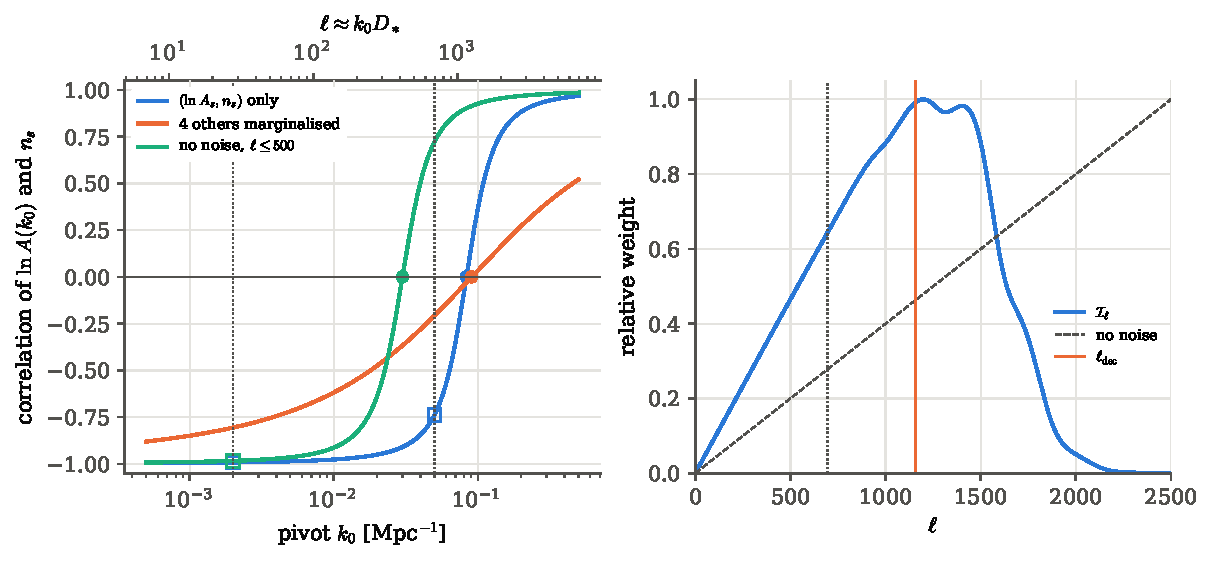
\includegraphics[width=12.5cm]{figures/ch08/pivot.pdf}
\caption{The pivot scale. Left: the correlation of $\ln A(k_0)$ and $n_s$ as a function of the
pivot $k_0$, for the Planck-like experiment with $(\ln A_s,n_s)$ alone (blue) and with the other
four parameters marginalised (orange), and for a noiseless spectrum cut at $\ell=500$ (green). The
curves follow from one Fisher matrix at $0.05\,{\rm Mpc}^{-1}$ moved along by \eqref{8a:eq:pivot-shift};
the open squares are Fisher matrices computed directly at each pivot, and the dots mark
$k_{\rm dec}$, where each curve crosses zero. The top axis converts $k_0$ to $\ell\approx k_0D_*$.
Right: the weight $\mathcal I_\ell$, the information on $\ln A_s$ per multipole, rises like $2\ell+1$ until
the beam and the noise cut it off; its weighted centre in $\ln\ell$ is $\ell_{\rm dec}$ (orange).
The dotted lines mark $0.002$ and $0.05\,{\rm Mpc}^{-1}$ (left) and $0.05\,{\rm Mpc}^{-1}$ (right).}
\label{8a:fig:pivot}
\end{figure}

\section{How it is done in research}
\label{8a:sec:research}

The toy pipeline of a beamed, noisy full sky has every structural element of a real temperature analysis
and almost none of its detail. It is worth seeing the real thing once, in the order in which
it runs, because every later chapter that uses $\Chat$ inherits its choices. The description
follows the Planck 2018 temperature analysis \cite{Planck2018V} and the MASTER method
\srcref{Hivon}{§3.6}, with modern implementations such as NaMaster \cite{Alonso2019}.

\paragraph{The data products.}
An analysis starts from the time-ordered data of every detector, with its pointing, and from
three calibrations made on the same data: the beam of each detector, measured by scanning
planets; the noise spectrum of each detector, measured from the timestream itself; and the
gain. Map-making turns the timestream into maps at $N_{\rm side}=2048$ for each high-frequency channel and
for each \emph{split} of the data (the two half-missions, two sets of detectors), together with
hit counts and pixel noise variances. Masks remove the Galaxy and bright point sources and
are apodised. The \emph{effective} beam window function of each map, which combines the beams of
the detectors that went into it with the way the scan crossed each pixel, is computed from
the beam measurements and the scan. Finally a large set of simulations is produced end to
end: CMB skies, foregrounds and noise timestreams, run through the same map-maker. In Planck
2018 these are the $300$ FFP10 realisations \cite{Planck2018V}.

\paragraph{The steps.}
\begin{enumerate}
  \item \emph{Maps.} Generalised least squares, or a destriper that removes the $1/f$ drifts,
        solves $\data=\mathsf A\bm s+\bm n$ for the map \srcref{HobsonBMC}{(10.10)--(10.13)}.
  \item \emph{Pseudo-spectra.} Each masked, apodised map is transformed; spectra are formed
        between \emph{different} splits, so that the noise bias never enters
        (\cref{8a:sec:cross}).
  \item \emph{Deconvolution.} The mode coupling of the mask is computed exactly from the
        mask's own spectrum and inverted in bins of $\ell$; the effective beam and pixel window
        are divided out \srcref{Hivon}{(14)--(26)}. A transfer function measured on noise-free
        simulations corrects for any filtering \srcref{Hivon}{(18)}.
  \item \emph{Covariance.} The covariance of the binned spectra, which a mask makes
        non-diagonal, is computed with analytic approximations for masked, noisy pseudo-spectra
        and checked on simulations, or estimated directly from simulations with the correction
        for a finite number of them \cite{Hartlap2007}.
  \item \emph{Likelihood.} Above $\ell=30$ the binned cross-spectra of the frequency maps
        enter a Gaussian likelihood together with foreground and instrument nuisance
        parameters, for $30\le\ell\le2508$ \cite{Planck2018V}. Below $\ell=30$, where the
        distribution is visibly a skewed $\chi^2$ (\cref{8a:sec:shape}), the likelihood is
        computed from the low-resolution map itself, with Gibbs sampling of the sky and the
        spectrum together \cite{Planck2018V}.
\end{enumerate}

\paragraph{The checks.}
None of this is trusted until it has passed tests designed to fail if something is wrong.
\emph{Null tests} difference two splits of the same sky: the signal cancels, and the spectrum
of the difference must be consistent with the noise model alone. \emph{Consistency tests}
compare spectra from different frequencies, detector sets and masks, which must agree after
foregrounds are accounted for. \emph{End-to-end tests} run the entire pipeline on the
simulations as if they were data and check that the input spectrum and parameters come back
without bias and with error bars that cover the truth as often as they claim
\cite{Planck2018V}. The full-sky checks of \cref{8a:sec:results} are the smallest version of
the last kind.

\begin{taxonomy}[Research pipeline and its laptop version]
\small
\begin{tabular}{@{}>{\raggedright\arraybackslash}p{2.0cm}>{\raggedright\arraybackslash}p{3.7cm}>{\raggedright\arraybackslash}p{3.2cm}>{\raggedright\arraybackslash}p{3.4cm}@{}}
step & research version & here & cost of the reduction \\
\hline
sky model & Gaussian CMB $+$ foregrounds, $N_{\rm side}=2048$ & Gaussian CMB, $N_{\rm side}=256$ & $\ell\le512$: $\EightAScaleModeFrac\%$ of the modes \\
beam & measured, asymmetric, per detector, with errors & circular Gaussian, $30'$ & no beam-error term \\
noise & correlated $1/f$ timestream through map-maker & white pixel noise (and one pattern) & no stripes or noise correlations \\
spectra & half-mission cross-spectra, masked & full sky, auto and cross & mask in the masked-sky analysis \\
simulations & $300$ end-to-end FFP10 & $\EightANsim$ Gaussian skies, $\EightAMinutes$\,min & MC error $\EightAScaleMCerrTwoK\%$ vs $\EightAScaleMCerrThree\%$, but less realism \\
full-scale run & computing cluster & extrapolated: $\EightAScaleHours$\,h for $1000$ Gaussian skies at $2048$ & breaks the $10$-minute budget \\
storage & maps on disk & spectra only, $29$\,MB & $1000$ maps at $2048$: $\EightAScaleDiskGB$\,GB \\
\end{tabular}
\end{taxonomy}

The reductions in the table are deliberate. Each removes something expensive whose effect
on the statistics of $\Chat$ is either known exactly on the full sky or is not the subject
here. What cannot be removed is the structure: random sky, deterministic instrument,
random noise, the same analysis on data and simulations, and statistics read off the
simulations. That structure is the same at $N_{\rm side}=256$ and at $2048$.

\begin{inpractice}[Verification and research with the same machine]
On the full sky the simulations \emph{verify}: every number they produced had an
analytic prediction, and agreement tested the code. In research the same loop is the
\emph{instrument}, used where no prediction exists: the transfer function of a filtered scan
\srcref{Hivon}{(18)}, the noise power of coloured, inhomogeneous, filtered noise
\srcref{Hivon}{§3.3}, and the covariance and distribution of the binned spectrum of a masked sky,
which the likelihood of \cref{ch:09} and the Fisher forecast of \cref{ch:10} need.
\end{inpractice}

The beam and the noise also change the map in ways the spectrum does not show. The beam
removes the smallest hot and cold spots, and the noise adds a grain of tiny new ones. Counts
of spots, their connectivity and the other shape statistics of \cref{ch:12} respond to both,
and the same simulations, which already produce beamed, noisy maps, will provide their
sampling distributions.

\begin{recap}
\begin{itemize}
  \item An instrument multiplies each $\alm$ by $T_\ell=B_\ell p_\ell$ (beam times pixel window,
        $B_\ell=e^{-\ell(\ell+1)\sigma_b^2/2}$ for a Gaussian beam) and adds noise after the
        smoothing; uniform white noise has $N_\ell=\sigma^2\Omega_{\rm pix}$ at every $\ell$, and
        any noise pattern has mean power $\Omega_{\rm pix}\langle\sigma^2\rangle$.
  \item The observed spectrum averages to $T_\ell^2\Cell+N_\ell$. Subtracting $N_\ell$ and dividing
        by $T_\ell^2$ gives an unbiased estimator, which on the full sky is the maximum-likelihood
        estimator and reaches the Cram\'er--Rao bound. Cross-spectra of independent halves need
        no noise subtraction and cost at most $\sqrt2$ in error.
  \item Its variance is $2(\Cell+N_\ell/T_\ell^2)^2/(2\ell+1)$ (Knox), its distribution a shifted,
        scaled $\chi^2_{2\ell+1}$, skewed at low $\ell$ and straddling zero where the noise
        dominates. The noise supplies half the variance once $N_\ell/(T_\ell^2\Cell)>\sqrt2-1$.
  \item The $\fsky$ version of the formula counts modes; it holds for wide bins with many modes
        and fails at low $\ell$ and small patches.
  \item The cumulative signal-to-noise $[\sum_\ell\SNR_\ell^2]^{1/2}$ is one over the error of an
        overall amplitude; it saturates a little beyond the multipole where noise and signal
        are equal.
  \item $\EightANsim$ simulated skies at $N_{\rm side}=256$, six minutes on a laptop, reproduce all
        of these to their Monte Carlo precision, and reproduce the full-sky content of Knox (1995)
        and Hivon et al.\ (2002) (\cref{8a:tab:literature}).
  \item An error bar needs about $50$ simulations for $10\%$ precision; a bias needs
        $(\sigma/\text{target})^2$.
\end{itemize}
\end{recap}
\providecommand{\EightBoneDfarSharp}{}\renewcommand{\EightBoneDfarSharp}{0.026}
\providecommand{\EightBoneDfarTaper}{}\renewcommand{\EightBoneDfarTaper}{1.6\times10^{-3}}
\providecommand{\EightBoneDkzero}{}\renewcommand{\EightBoneDkzero}{40}
\providecommand{\EightBfskyFull}{}\renewcommand{\EightBfskyFull}{1.000}
\providecommand{\EightBwtwoFull}{}\renewcommand{\EightBwtwoFull}{1.000}
\providecommand{\EightBwfourFull}{}\renewcommand{\EightBwfourFull}{1.000}
\providecommand{\EightBweffFull}{}\renewcommand{\EightBweffFull}{1.000}
\providecommand{\EightBfeffFull}{}\renewcommand{\EightBfeffFull}{1.000}
\providecommand{\EightBParsevalFull}{}\renewcommand{\EightBParsevalFull}{1.0000}
\providecommand{\EightBWzeroFull}{}\renewcommand{\EightBWzeroFull}{1.776\times10^{-15}}
\providecommand{\EightBfskyCapTen}{}\renewcommand{\EightBfskyCapTen}{0.100}
\providecommand{\EightBwtwoCapTen}{}\renewcommand{\EightBwtwoCapTen}{1.000}
\providecommand{\EightBwfourCapTen}{}\renewcommand{\EightBwfourCapTen}{1.000}
\providecommand{\EightBweffCapTen}{}\renewcommand{\EightBweffCapTen}{1.000}
\providecommand{\EightBfeffCapTen}{}\renewcommand{\EightBfeffCapTen}{0.100}
\providecommand{\EightBParsevalCapTen}{}\renewcommand{\EightBParsevalCapTen}{0.9995}
\providecommand{\EightBWzeroCapTen}{}\renewcommand{\EightBWzeroCapTen}{2.220\times10^{-16}}
\providecommand{\EightBfskyCapTenApo}{}\renewcommand{\EightBfskyCapTenApo}{0.100}
\providecommand{\EightBwtwoCapTenApo}{}\renewcommand{\EightBwtwoCapTenApo}{0.698}
\providecommand{\EightBwfourCapTenApo}{}\renewcommand{\EightBwfourCapTenApo}{0.653}
\providecommand{\EightBweffCapTenApo}{}\renewcommand{\EightBweffCapTenApo}{0.746}
\providecommand{\EightBfeffCapTenApo}{}\renewcommand{\EightBfeffCapTenApo}{0.075}
\providecommand{\EightBParsevalCapTenApo}{}\renewcommand{\EightBParsevalCapTenApo}{1.0000}
\providecommand{\EightBWzeroCapTenApo}{}\renewcommand{\EightBWzeroCapTenApo}{2.220\times10^{-16}}
\providecommand{\EightBfskyCapThirty}{}\renewcommand{\EightBfskyCapThirty}{0.300}
\providecommand{\EightBwtwoCapThirty}{}\renewcommand{\EightBwtwoCapThirty}{1.000}
\providecommand{\EightBwfourCapThirty}{}\renewcommand{\EightBwfourCapThirty}{1.000}
\providecommand{\EightBweffCapThirty}{}\renewcommand{\EightBweffCapThirty}{1.000}
\providecommand{\EightBfeffCapThirty}{}\renewcommand{\EightBfeffCapThirty}{0.300}
\providecommand{\EightBParsevalCapThirty}{}\renewcommand{\EightBParsevalCapThirty}{0.9996}
\providecommand{\EightBWzeroCapThirty}{}\renewcommand{\EightBWzeroCapThirty}{4.441\times10^{-16}}
\providecommand{\EightBfskyCapSeventy}{}\renewcommand{\EightBfskyCapSeventy}{0.700}
\providecommand{\EightBwtwoCapSeventy}{}\renewcommand{\EightBwtwoCapSeventy}{1.000}
\providecommand{\EightBwfourCapSeventy}{}\renewcommand{\EightBwfourCapSeventy}{1.000}
\providecommand{\EightBweffCapSeventy}{}\renewcommand{\EightBweffCapSeventy}{1.000}
\providecommand{\EightBfeffCapSeventy}{}\renewcommand{\EightBfeffCapSeventy}{0.700}
\providecommand{\EightBParsevalCapSeventy}{}\renewcommand{\EightBParsevalCapSeventy}{0.9998}
\providecommand{\EightBWzeroCapSeventy}{}\renewcommand{\EightBWzeroCapSeventy}{1.998\times10^{-15}}
\providecommand{\EightBfskyBand}{}\renewcommand{\EightBfskyBand}{0.658}
\providecommand{\EightBwtwoBand}{}\renewcommand{\EightBwtwoBand}{1.000}
\providecommand{\EightBwfourBand}{}\renewcommand{\EightBwfourBand}{1.000}
\providecommand{\EightBweffBand}{}\renewcommand{\EightBweffBand}{1.000}
\providecommand{\EightBfeffBand}{}\renewcommand{\EightBfeffBand}{0.658}
\providecommand{\EightBParsevalBand}{}\renewcommand{\EightBParsevalBand}{0.9996}
\providecommand{\EightBWzeroBand}{}\renewcommand{\EightBWzeroBand}{2.220\times10^{-16}}
\providecommand{\EightBfskyBandApo}{}\renewcommand{\EightBfskyBandApo}{0.658}
\providecommand{\EightBwtwoBandApo}{}\renewcommand{\EightBwtwoBandApo}{0.924}
\providecommand{\EightBwfourBandApo}{}\renewcommand{\EightBwfourBandApo}{0.911}
\providecommand{\EightBweffBandApo}{}\renewcommand{\EightBweffBandApo}{0.936}
\providecommand{\EightBfeffBandApo}{}\renewcommand{\EightBfeffBandApo}{0.616}
\providecommand{\EightBParsevalBandApo}{}\renewcommand{\EightBParsevalBandApo}{1.0000}
\providecommand{\EightBWzeroBandApo}{}\renewcommand{\EightBWzeroBandApo}{0}
\providecommand{\EightBfskyHoles}{}\renewcommand{\EightBfskyHoles}{0.970}
\providecommand{\EightBwtwoHoles}{}\renewcommand{\EightBwtwoHoles}{1.000}
\providecommand{\EightBwfourHoles}{}\renewcommand{\EightBwfourHoles}{1.000}
\providecommand{\EightBweffHoles}{}\renewcommand{\EightBweffHoles}{1.000}
\providecommand{\EightBfeffHoles}{}\renewcommand{\EightBfeffHoles}{0.970}
\providecommand{\EightBParsevalHoles}{}\renewcommand{\EightBParsevalHoles}{0.9995}
\providecommand{\EightBWzeroHoles}{}\renewcommand{\EightBWzeroHoles}{4.441\times10^{-16}}
\providecommand{\EightBfskyBandExact}{}\renewcommand{\EightBfskyBandExact}{0.6580}
\providecommand{\EightBfskyBandPix}{}\renewcommand{\EightBfskyBandPix}{0.6576}
\providecommand{\EightBcapTenDeg}{}\renewcommand{\EightBcapTenDeg}{36.87}
\providecommand{\EightBcapThirtyDeg}{}\renewcommand{\EightBcapThirtyDeg}{66.42}
\providecommand{\EightBcapSeventyDeg}{}\renewcommand{\EightBcapSeventyDeg}{113.58}
\providecommand{\EightBholesNaive}{}\renewcommand{\EightBholesNaive}{0.0305}
\providecommand{\EightBholesLost}{}\renewcommand{\EightBholesLost}{0.0301}
\providecommand{\EightBnside}{}\renewcommand{\EightBnside}{256}
\providecommand{\EightBthreejWorst}{}\renewcommand{\EightBthreejWorst}{1.026\times10^{-12}}
\providecommand{\EightBthreejExample}{}\renewcommand{\EightBthreejExample}{0.057143}
\providecommand{\EightBorthSum}{}\renewcommand{\EightBorthSum}{1.000000000000}
\providecommand{\EightBrowRuleFull}{}\renewcommand{\EightBrowRuleFull}{4.1\times10^{-6}}
\providecommand{\EightBfarLeakFull}{}\renewcommand{\EightBfarLeakFull}{3.5\times10^{-5}}
\providecommand{\EightBcondFull}{}\renewcommand{\EightBcondFull}{1.1}
\providecommand{\EightBrowRuleCapTen}{}\renewcommand{\EightBrowRuleCapTen}{8.0\times10^{-4}}
\providecommand{\EightBfarLeakCapTen}{}\renewcommand{\EightBfarLeakCapTen}{2.9}
\providecommand{\EightBcondCapTen}{}\renewcommand{\EightBcondCapTen}{1.3\times10^{17}}
\providecommand{\EightBrowRuleCapTenApo}{}\renewcommand{\EightBrowRuleCapTenApo}{2.4\times10^{-5}}
\providecommand{\EightBfarLeakCapTenApo}{}\renewcommand{\EightBfarLeakCapTenApo}{0.33}
\providecommand{\EightBcondCapTenApo}{}\renewcommand{\EightBcondCapTenApo}{5.8\times10^{16}}
\providecommand{\EightBrowRuleCapThirty}{}\renewcommand{\EightBrowRuleCapThirty}{4.9\times10^{-4}}
\providecommand{\EightBfarLeakCapThirty}{}\renewcommand{\EightBfarLeakCapThirty}{1.5}
\providecommand{\EightBcondCapThirty}{}\renewcommand{\EightBcondCapThirty}{1.3\times10^{16}}
\providecommand{\EightBrowRuleCapSeventy}{}\renewcommand{\EightBrowRuleCapSeventy}{2.1\times10^{-4}}
\providecommand{\EightBfarLeakCapSeventy}{}\renewcommand{\EightBfarLeakCapSeventy}{0.63}
\providecommand{\EightBcondCapSeventy}{}\renewcommand{\EightBcondCapSeventy}{1.8}
\providecommand{\EightBrowRuleBand}{}\renewcommand{\EightBrowRuleBand}{4.5\times10^{-4}}
\providecommand{\EightBfarLeakBand}{}\renewcommand{\EightBfarLeakBand}{1.3}
\providecommand{\EightBcondBand}{}\renewcommand{\EightBcondBand}{1.8}
\providecommand{\EightBrowRuleBandApo}{}\renewcommand{\EightBrowRuleBandApo}{6.8\times10^{-6}}
\providecommand{\EightBfarLeakBandApo}{}\renewcommand{\EightBfarLeakBandApo}{0.44}
\providecommand{\EightBcondBandApo}{}\renewcommand{\EightBcondBandApo}{2}
\providecommand{\EightBrowRuleHoles}{}\renewcommand{\EightBrowRuleHoles}{7.0\times10^{-4}}
\providecommand{\EightBfarLeakHoles}{}\renewcommand{\EightBfarLeakHoles}{2.3}
\providecommand{\EightBcondHoles}{}\renewcommand{\EightBcondHoles}{1.1}
\providecommand{\EightBNsim}{}\renewcommand{\EightBNsim}{2000}
\providecommand{\EightBSecPerSky}{}\renewcommand{\EightBSecPerSky}{0.66}
\providecommand{\EightBCPUMinutes}{}\renewcommand{\EightBCPUMinutes}{22}
\providecommand{\EightBNmasks}{}\renewcommand{\EightBNmasks}{8}
\providecommand{\EightBdirectWorst}{}\renewcommand{\EightBdirectWorst}{8.5\times10^{-13}}
\providecommand{\EightBpullchiFull}{}\renewcommand{\EightBpullchiFull}{1.05}
\providecommand{\EightBpullmeanFull}{}\renewcommand{\EightBpullmeanFull}{+0.01}
\providecommand{\EightBpullchiCapTen}{}\renewcommand{\EightBpullchiCapTen}{0.87}
\providecommand{\EightBpullmeanCapTen}{}\renewcommand{\EightBpullmeanCapTen}{+0.20}
\providecommand{\EightBpullchiCapTenApo}{}\renewcommand{\EightBpullchiCapTenApo}{0.81}
\providecommand{\EightBpullmeanCapTenApo}{}\renewcommand{\EightBpullmeanCapTenApo}{+0.03}
\providecommand{\EightBpullchiCapThirty}{}\renewcommand{\EightBpullchiCapThirty}{1.04}
\providecommand{\EightBpullmeanCapThirty}{}\renewcommand{\EightBpullmeanCapThirty}{+0.03}
\providecommand{\EightBpullchiCapSeventy}{}\renewcommand{\EightBpullchiCapSeventy}{1.00}
\providecommand{\EightBpullmeanCapSeventy}{}\renewcommand{\EightBpullmeanCapSeventy}{+0.10}
\providecommand{\EightBpullchiBand}{}\renewcommand{\EightBpullchiBand}{1.06}
\providecommand{\EightBpullmeanBand}{}\renewcommand{\EightBpullmeanBand}{+0.11}
\providecommand{\EightBpullchiBandApo}{}\renewcommand{\EightBpullchiBandApo}{1.07}
\providecommand{\EightBpullmeanBandApo}{}\renewcommand{\EightBpullmeanBandApo}{+0.04}
\providecommand{\EightBpullchiHoles}{}\renewcommand{\EightBpullchiHoles}{1.07}
\providecommand{\EightBpullmeanHoles}{}\renewcommand{\EightBpullmeanHoles}{+0.19}
\providecommand{\EightBLchk}{}\renewcommand{\EightBLchk}{600}
\providecommand{\EightBLrep}{}\renewcommand{\EightBLrep}{600}
\providecommand{\EightBnullCapTen}{}\renewcommand{\EightBnullCapTen}{59}
\providecommand{\EightBnullCapThirty}{}\renewcommand{\EightBnullCapThirty}{27}
\providecommand{\EightBnullCapSeventy}{}\renewcommand{\EightBnullCapSeventy}{0}
\providecommand{\EightBnullBand}{}\renewcommand{\EightBnullBand}{0}
\providecommand{\EightBnullHoles}{}\renewcommand{\EightBnullHoles}{0}
\providecommand{\EightBnaiveBiasLowFull}{}\renewcommand{\EightBnaiveBiasLowFull}{+0}
\providecommand{\EightBnaiveBiasMaxFull}{}\renewcommand{\EightBnaiveBiasMaxFull}{0}
\providecommand{\EightBmasterPullBinFull}{}\renewcommand{\EightBmasterPullBinFull}{10.8}
\providecommand{\EightBmasterPullWinFull}{}\renewcommand{\EightBmasterPullWinFull}{2.7}
\providecommand{\EightBmasterBiasSigFull}{}\renewcommand{\EightBmasterBiasSigFull}{0.24}
\providecommand{\EightBcondKFull}{}\renewcommand{\EightBcondKFull}{7.3e+03}
\providecommand{\EightBnaiveBiasLowCapTen}{}\renewcommand{\EightBnaiveBiasLowCapTen}{+4}
\providecommand{\EightBnaiveBiasMaxCapTen}{}\renewcommand{\EightBnaiveBiasMaxCapTen}{112}
\providecommand{\EightBmasterPullBinCapTen}{}\renewcommand{\EightBmasterPullBinCapTen}{3.4}
\providecommand{\EightBmasterPullWinCapTen}{}\renewcommand{\EightBmasterPullWinCapTen}{2.0}
\providecommand{\EightBmasterBiasSigCapTen}{}\renewcommand{\EightBmasterBiasSigCapTen}{0.08}
\providecommand{\EightBcondKCapTen}{}\renewcommand{\EightBcondKCapTen}{1.2\times10^{4}}
\providecommand{\EightBnaiveBiasLowCapTenApo}{}\renewcommand{\EightBnaiveBiasLowCapTenApo}{+7}
\providecommand{\EightBnaiveBiasMaxCapTenApo}{}\renewcommand{\EightBnaiveBiasMaxCapTenApo}{7}
\providecommand{\EightBmasterPullBinCapTenApo}{}\renewcommand{\EightBmasterPullBinCapTenApo}{3.9}
\providecommand{\EightBmasterPullWinCapTenApo}{}\renewcommand{\EightBmasterPullWinCapTenApo}{1.9}
\providecommand{\EightBmasterBiasSigCapTenApo}{}\renewcommand{\EightBmasterBiasSigCapTenApo}{0.09}
\providecommand{\EightBcondKCapTenApo}{}\renewcommand{\EightBcondKCapTenApo}{1.2\times10^{4}}
\providecommand{\EightBnaiveBiasLowCapThirty}{}\renewcommand{\EightBnaiveBiasLowCapThirty}{+2}
\providecommand{\EightBnaiveBiasMaxCapThirty}{}\renewcommand{\EightBnaiveBiasMaxCapThirty}{52}
\providecommand{\EightBmasterPullBinCapThirty}{}\renewcommand{\EightBmasterPullBinCapThirty}{4.6}
\providecommand{\EightBmasterPullWinCapThirty}{}\renewcommand{\EightBmasterPullWinCapThirty}{2.2}
\providecommand{\EightBmasterBiasSigCapThirty}{}\renewcommand{\EightBmasterBiasSigCapThirty}{0.10}
\providecommand{\EightBcondKCapThirty}{}\renewcommand{\EightBcondKCapThirty}{9.5e+03}
\providecommand{\EightBnaiveBiasLowCapSeventy}{}\renewcommand{\EightBnaiveBiasLowCapSeventy}{+1}
\providecommand{\EightBnaiveBiasMaxCapSeventy}{}\renewcommand{\EightBnaiveBiasMaxCapSeventy}{22}
\providecommand{\EightBmasterPullBinCapSeventy}{}\renewcommand{\EightBmasterPullBinCapSeventy}{7.3}
\providecommand{\EightBmasterPullWinCapSeventy}{}\renewcommand{\EightBmasterPullWinCapSeventy}{2.6}
\providecommand{\EightBmasterBiasSigCapSeventy}{}\renewcommand{\EightBmasterBiasSigCapSeventy}{0.16}
\providecommand{\EightBcondKCapSeventy}{}\renewcommand{\EightBcondKCapSeventy}{8.1e+03}
\providecommand{\EightBnaiveBiasLowBand}{}\renewcommand{\EightBnaiveBiasLowBand}{+2}
\providecommand{\EightBnaiveBiasMaxBand}{}\renewcommand{\EightBnaiveBiasMaxBand}{49}
\providecommand{\EightBmasterPullBinBand}{}\renewcommand{\EightBmasterPullBinBand}{7.5}
\providecommand{\EightBmasterPullWinBand}{}\renewcommand{\EightBmasterPullWinBand}{3.2}
\providecommand{\EightBmasterBiasSigBand}{}\renewcommand{\EightBmasterBiasSigBand}{0.17}
\providecommand{\EightBcondKBand}{}\renewcommand{\EightBcondKBand}{8.9e+03}
\providecommand{\EightBnaiveBiasLowBandApo}{}\renewcommand{\EightBnaiveBiasLowBandApo}{+3}
\providecommand{\EightBnaiveBiasMaxBandApo}{}\renewcommand{\EightBnaiveBiasMaxBandApo}{3}
\providecommand{\EightBmasterPullBinBandApo}{}\renewcommand{\EightBmasterPullBinBandApo}{6.9}
\providecommand{\EightBmasterPullWinBandApo}{}\renewcommand{\EightBmasterPullWinBandApo}{3.0}
\providecommand{\EightBmasterBiasSigBandApo}{}\renewcommand{\EightBmasterBiasSigBandApo}{0.15}
\providecommand{\EightBcondKBandApo}{}\renewcommand{\EightBcondKBandApo}{8.9e+03}
\providecommand{\EightBnaiveBiasLowHoles}{}\renewcommand{\EightBnaiveBiasLowHoles}{-2}
\providecommand{\EightBnaiveBiasMaxHoles}{}\renewcommand{\EightBnaiveBiasMaxHoles}{122}
\providecommand{\EightBmasterPullBinHoles}{}\renewcommand{\EightBmasterPullBinHoles}{11.8}
\providecommand{\EightBmasterPullWinHoles}{}\renewcommand{\EightBmasterPullWinHoles}{3.0}
\providecommand{\EightBmasterBiasSigHoles}{}\renewcommand{\EightBmasterBiasSigHoles}{0.26}
\providecommand{\EightBcondKHoles}{}\renewcommand{\EightBcondKHoles}{7.5e+03}
\providecommand{\EightBNF}{}\renewcommand{\EightBNF}{500}
\providecommand{\EightBNtest}{}\renewcommand{\EightBNtest}{1500}
\providecommand{\EightBFbinOne}{}\renewcommand{\EightBFbinOne}{0.88}
\providecommand{\EightBFbinTwo}{}\renewcommand{\EightBFbinTwo}{0.97}
\providecommand{\EightBFbinFive}{}\renewcommand{\EightBFbinFive}{0.991}
\providecommand{\EightBFbinHigh}{}\renewcommand{\EightBFbinHigh}{1.000}
\providecommand{\EightBFoneHigh}{}\renewcommand{\EightBFoneHigh}{1.06}
\providecommand{\EightBFzeroHigh}{}\renewcommand{\EightBFzeroHigh}{1.26}
\providecommand{\EightBdFratio}{}\renewcommand{\EightBdFratio}{1.55}
\providecommand{\EightBdFratioErr}{}\renewcommand{\EightBdFratioErr}{0.13}
\providecommand{\EightBdFgroups}{}\renewcommand{\EightBdFgroups}{4}
\providecommand{\EightBfiltWithoutLow}{}\renewcommand{\EightBfiltWithoutLow}{-13}
\providecommand{\EightBfiltWithoutTwo}{}\renewcommand{\EightBfiltWithoutTwo}{-3.6}
\providecommand{\EightBfiltWithLow}{}\renewcommand{\EightBfiltWithLow}{-1.3}
\providecommand{\EightBfiltWithPull}{}\renewcommand{\EightBfiltWithPull}{5.0}
\providecommand{\EightBfiltWithBiasSig}{}\renewcommand{\EightBfiltWithBiasSig}{0.13}
\providecommand{\EightBbelowFullTwo}{}\renewcommand{\EightBbelowFullTwo}{0.58}
\providecommand{\EightBnueffFullTwo}{}\renewcommand{\EightBnueffFullTwo}{4.7}
\providecommand{\EightBksFullTwo}{}\renewcommand{\EightBksFullTwo}{0.034}
\providecommand{\EightBksgFullTwo}{}\renewcommand{\EightBksgFullTwo}{0.115}
\providecommand{\EightBbelowFullTen}{}\renewcommand{\EightBbelowFullTen}{0.53}
\providecommand{\EightBnueffFullTen}{}\renewcommand{\EightBnueffFullTen}{20.7}
\providecommand{\EightBksFullTen}{}\renewcommand{\EightBksFullTen}{0.042}
\providecommand{\EightBksgFullTen}{}\renewcommand{\EightBksgFullTen}{0.065}
\providecommand{\EightBbelowFullFifty}{}\renewcommand{\EightBbelowFullFifty}{0.53}
\providecommand{\EightBnueffFullFifty}{}\renewcommand{\EightBnueffFullFifty}{102.3}
\providecommand{\EightBksFullFifty}{}\renewcommand{\EightBksFullFifty}{0.059}
\providecommand{\EightBksgFullFifty}{}\renewcommand{\EightBksgFullFifty}{0.049}
\providecommand{\EightBbelowCapThirtyTwo}{}\renewcommand{\EightBbelowCapThirtyTwo}{0.60}
\providecommand{\EightBnueffCapThirtyTwo}{}\renewcommand{\EightBnueffCapThirtyTwo}{3.8}
\providecommand{\EightBksCapThirtyTwo}{}\renewcommand{\EightBksCapThirtyTwo}{0.022}
\providecommand{\EightBksgCapThirtyTwo}{}\renewcommand{\EightBksgCapThirtyTwo}{0.117}
\providecommand{\EightBbelowCapThirtyTen}{}\renewcommand{\EightBbelowCapThirtyTen}{0.54}
\providecommand{\EightBnueffCapThirtyTen}{}\renewcommand{\EightBnueffCapThirtyTen}{17.6}
\providecommand{\EightBksCapThirtyTen}{}\renewcommand{\EightBksCapThirtyTen}{0.017}
\providecommand{\EightBksgCapThirtyTen}{}\renewcommand{\EightBksgCapThirtyTen}{0.051}
\providecommand{\EightBbelowCapThirtyFifty}{}\renewcommand{\EightBbelowCapThirtyFifty}{0.52}
\providecommand{\EightBnueffCapThirtyFifty}{}\renewcommand{\EightBnueffCapThirtyFifty}{93.4}
\providecommand{\EightBksCapThirtyFifty}{}\renewcommand{\EightBksCapThirtyFifty}{0.050}
\providecommand{\EightBksgCapThirtyFifty}{}\renewcommand{\EightBksgCapThirtyFifty}{0.044}
\providecommand{\EightBbelowCapTenTwo}{}\renewcommand{\EightBbelowCapTenTwo}{0.64}
\providecommand{\EightBnueffCapTenTwo}{}\renewcommand{\EightBnueffCapTenTwo}{2.1}
\providecommand{\EightBksCapTenTwo}{}\renewcommand{\EightBksCapTenTwo}{0.066}
\providecommand{\EightBksgCapTenTwo}{}\renewcommand{\EightBksgCapTenTwo}{0.167}
\providecommand{\EightBbelowCapTenTen}{}\renewcommand{\EightBbelowCapTenTen}{0.57}
\providecommand{\EightBnueffCapTenTen}{}\renewcommand{\EightBnueffCapTenTen}{9.7}
\providecommand{\EightBksCapTenTen}{}\renewcommand{\EightBksCapTenTen}{0.034}
\providecommand{\EightBksgCapTenTen}{}\renewcommand{\EightBksgCapTenTen}{0.095}
\providecommand{\EightBbelowCapTenFifty}{}\renewcommand{\EightBbelowCapTenFifty}{0.52}
\providecommand{\EightBnueffCapTenFifty}{}\renewcommand{\EightBnueffCapTenFifty}{57.1}
\providecommand{\EightBksCapTenFifty}{}\renewcommand{\EightBksCapTenFifty}{0.033}
\providecommand{\EightBksgCapTenFifty}{}\renewcommand{\EightBksgCapTenFifty}{0.020}
\providecommand{\EightBksNtest}{}\renewcommand{\EightBksNtest}{1000}
\providecommand{\EightBksCrit}{}\renewcommand{\EightBksCrit}{0.060}
\providecommand{\EightBksCritMin}{}\renewcommand{\EightBksCritMin}{0.049}
\providecommand{\EightBksNboot}{}\renewcommand{\EightBksNboot}{300}
\providecommand{\EightBnuratioFullTwo}{}\renewcommand{\EightBnuratioFullTwo}{0.94}
\providecommand{\EightBnuratioFullTen}{}\renewcommand{\EightBnuratioFullTen}{0.98}
\providecommand{\EightBnuratioFullHundred}{}\renewcommand{\EightBnuratioFullHundred}{1.05}
\providecommand{\EightBnuratioFullFivehundred}{}\renewcommand{\EightBnuratioFullFivehundred}{0.99}
\providecommand{\EightBnuratioHighFull}{}\renewcommand{\EightBnuratioHighFull}{1.00}
\providecommand{\EightBnuratioCapSeventyTwo}{}\renewcommand{\EightBnuratioCapSeventyTwo}{1.26}
\providecommand{\EightBnuratioCapSeventyTen}{}\renewcommand{\EightBnuratioCapSeventyTen}{1.45}
\providecommand{\EightBnuratioCapSeventyHundred}{}\renewcommand{\EightBnuratioCapSeventyHundred}{1.49}
\providecommand{\EightBnuratioCapSeventyFivehundred}{}\renewcommand{\EightBnuratioCapSeventyFivehundred}{1.39}
\providecommand{\EightBnuratioHighCapSeventy}{}\renewcommand{\EightBnuratioHighCapSeventy}{1.40}
\providecommand{\EightBnuratioCapThirtyTwo}{}\renewcommand{\EightBnuratioCapThirtyTwo}{2.55}
\providecommand{\EightBnuratioCapThirtyTen}{}\renewcommand{\EightBnuratioCapThirtyTen}{2.79}
\providecommand{\EightBnuratioCapThirtyHundred}{}\renewcommand{\EightBnuratioCapThirtyHundred}{3.04}
\providecommand{\EightBnuratioCapThirtyFivehundred}{}\renewcommand{\EightBnuratioCapThirtyFivehundred}{2.85}
\providecommand{\EightBnuratioHighCapThirty}{}\renewcommand{\EightBnuratioHighCapThirty}{2.90}
\providecommand{\EightBnuratioCapTenTwo}{}\renewcommand{\EightBnuratioCapTenTwo}{4.16}
\providecommand{\EightBnuratioCapTenTen}{}\renewcommand{\EightBnuratioCapTenTen}{4.62}
\providecommand{\EightBnuratioCapTenHundred}{}\renewcommand{\EightBnuratioCapTenHundred}{5.79}
\providecommand{\EightBnuratioCapTenFivehundred}{}\renewcommand{\EightBnuratioCapTenFivehundred}{5.02}
\providecommand{\EightBnuratioHighCapTen}{}\renewcommand{\EightBnuratioHighCapTen}{5.21}
\providecommand{\EightBnuratioCapTenApoTwo}{}\renewcommand{\EightBnuratioCapTenApoTwo}{4.40}
\providecommand{\EightBnuratioCapTenApoTen}{}\renewcommand{\EightBnuratioCapTenApoTen}{5.46}
\providecommand{\EightBnuratioCapTenApoHundred}{}\renewcommand{\EightBnuratioCapTenApoHundred}{6.61}
\providecommand{\EightBnuratioCapTenApoFivehundred}{}\renewcommand{\EightBnuratioCapTenApoFivehundred}{6.34}
\providecommand{\EightBnuratioHighCapTenApo}{}\renewcommand{\EightBnuratioHighCapTenApo}{6.42}
\providecommand{\EightBnuratioBandTwo}{}\renewcommand{\EightBnuratioBandTwo}{1.12}
\providecommand{\EightBnuratioBandTen}{}\renewcommand{\EightBnuratioBandTen}{1.27}
\providecommand{\EightBnuratioBandHundred}{}\renewcommand{\EightBnuratioBandHundred}{1.35}
\providecommand{\EightBnuratioBandFivehundred}{}\renewcommand{\EightBnuratioBandFivehundred}{1.42}
\providecommand{\EightBnuratioHighBand}{}\renewcommand{\EightBnuratioHighBand}{1.36}
\providecommand{\EightBnuratioHolesTwo}{}\renewcommand{\EightBnuratioHolesTwo}{0.97}
\providecommand{\EightBnuratioHolesTen}{}\renewcommand{\EightBnuratioHolesTen}{1.02}
\providecommand{\EightBnuratioHolesHundred}{}\renewcommand{\EightBnuratioHolesHundred}{1.09}
\providecommand{\EightBnuratioHolesFivehundred}{}\renewcommand{\EightBnuratioHolesFivehundred}{0.98}
\providecommand{\EightBnuratioHighHoles}{}\renewcommand{\EightBnuratioHighHoles}{1.02}
\providecommand{\EightBcorrOneCapSeventy}{}\renewcommand{\EightBcorrOneCapSeventy}{0.13}
\providecommand{\EightBcorrTwoCapSeventy}{}\renewcommand{\EightBcorrTwoCapSeventy}{0.03}
\providecommand{\EightBcorrOneCapThirty}{}\renewcommand{\EightBcorrOneCapThirty}{0.65}
\providecommand{\EightBcorrTwoCapThirty}{}\renewcommand{\EightBcorrTwoCapThirty}{0.14}
\providecommand{\EightBcorrOneCapTen}{}\renewcommand{\EightBcorrOneCapTen}{0.88}
\providecommand{\EightBcorrTwoCapTen}{}\renewcommand{\EightBcorrTwoCapTen}{0.60}
\providecommand{\EightBcorrOneCapTenApo}{}\renewcommand{\EightBcorrOneCapTenApo}{0.92}
\providecommand{\EightBcorrTwoCapTenApo}{}\renewcommand{\EightBcorrTwoCapTenApo}{0.72}
\providecommand{\EightBcorrOneBand}{}\renewcommand{\EightBcorrOneBand}{-0.00}
\providecommand{\EightBcorrTwoBand}{}\renewcommand{\EightBcorrTwoBand}{0.11}
\providecommand{\EightBcorrOneHoles}{}\renewcommand{\EightBcorrOneHoles}{-0.00}
\providecommand{\EightBcorrTwoHoles}{}\renewcommand{\EightBcorrTwoHoles}{-0.00}
\providecommand{\EightBcorrNoise}{}\renewcommand{\EightBcorrNoise}{0.022}
\providecommand{\EightBknoxFirstFull}{}\renewcommand{\EightBknoxFirstFull}{1.05}
\providecommand{\EightBknoxSecondFull}{}\renewcommand{\EightBknoxSecondFull}{1.00}
\providecommand{\EightBknoxHighFull}{}\renewcommand{\EightBknoxHighFull}{1.00}
\providecommand{\EightBknoxOnlyHighFull}{}\renewcommand{\EightBknoxOnlyHighFull}{1.00}
\providecommand{\EightBknoxFirstCapSeventy}{}\renewcommand{\EightBknoxFirstCapSeventy}{1.06}
\providecommand{\EightBknoxSecondCapSeventy}{}\renewcommand{\EightBknoxSecondCapSeventy}{1.07}
\providecommand{\EightBknoxHighCapSeventy}{}\renewcommand{\EightBknoxHighCapSeventy}{1.08}
\providecommand{\EightBknoxOnlyHighCapSeventy}{}\renewcommand{\EightBknoxOnlyHighCapSeventy}{1.08}
\providecommand{\EightBknoxFirstCapThirty}{}\renewcommand{\EightBknoxFirstCapThirty}{1.05}
\providecommand{\EightBknoxSecondCapThirty}{}\renewcommand{\EightBknoxSecondCapThirty}{1.14}
\providecommand{\EightBknoxHighCapThirty}{}\renewcommand{\EightBknoxHighCapThirty}{1.18}
\providecommand{\EightBknoxOnlyHighCapThirty}{}\renewcommand{\EightBknoxOnlyHighCapThirty}{1.18}
\providecommand{\EightBknoxFirstCapTen}{}\renewcommand{\EightBknoxFirstCapTen}{1.00}
\providecommand{\EightBknoxSecondCapTen}{}\renewcommand{\EightBknoxSecondCapTen}{1.36}
\providecommand{\EightBknoxHighCapTen}{}\renewcommand{\EightBknoxHighCapTen}{1.40}
\providecommand{\EightBknoxOnlyHighCapTen}{}\renewcommand{\EightBknoxOnlyHighCapTen}{1.40}
\providecommand{\EightBknoxFirstCapTenApo}{}\renewcommand{\EightBknoxFirstCapTenApo}{0.97}
\providecommand{\EightBknoxSecondCapTenApo}{}\renewcommand{\EightBknoxSecondCapTenApo}{1.22}
\providecommand{\EightBknoxHighCapTenApo}{}\renewcommand{\EightBknoxHighCapTenApo}{1.15}
\providecommand{\EightBknoxOnlyHighCapTenApo}{}\renewcommand{\EightBknoxOnlyHighCapTenApo}{1.54}
\providecommand{\EightBknoxFirstBand}{}\renewcommand{\EightBknoxFirstBand}{1.12}
\providecommand{\EightBknoxSecondBand}{}\renewcommand{\EightBknoxSecondBand}{1.16}
\providecommand{\EightBknoxHighBand}{}\renewcommand{\EightBknoxHighBand}{1.18}
\providecommand{\EightBknoxOnlyHighBand}{}\renewcommand{\EightBknoxOnlyHighBand}{1.18}
\providecommand{\EightBknoxFirstHoles}{}\renewcommand{\EightBknoxFirstHoles}{1.03}
\providecommand{\EightBknoxSecondHoles}{}\renewcommand{\EightBknoxSecondHoles}{1.00}
\providecommand{\EightBknoxHighHoles}{}\renewcommand{\EightBknoxHighHoles}{1.33}
\providecommand{\EightBknoxOnlyHighHoles}{}\renewcommand{\EightBknoxOnlyHighHoles}{1.33}
\providecommand{\EightBvarNoise}{}\renewcommand{\EightBvarNoise}{3.2}
\providecommand{\EightBefsTwoCapSeventy}{}\renewcommand{\EightBefsTwoCapSeventy}{1.44}
\providecommand{\EightBefsTenCapSeventy}{}\renewcommand{\EightBefsTenCapSeventy}{0.98}
\providecommand{\EightBefsHighCapSeventy}{}\renewcommand{\EightBefsHighCapSeventy}{0.976}
\providecommand{\EightBimpTwoCapSeventy}{}\renewcommand{\EightBimpTwoCapSeventy}{0.89}
\providecommand{\EightBimpTenCapSeventy}{}\renewcommand{\EightBimpTenCapSeventy}{1.04}
\providecommand{\EightBimpHighCapSeventy}{}\renewcommand{\EightBimpHighCapSeventy}{1.004}
\providecommand{\EightBefsBinFirstCapSeventy}{}\renewcommand{\EightBefsBinFirstCapSeventy}{0.90}
\providecommand{\EightBefsBinHighCapSeventy}{}\renewcommand{\EightBefsBinHighCapSeventy}{0.972}
\providecommand{\EightBefsTwoCapThirty}{}\renewcommand{\EightBefsTwoCapThirty}{3.34}
\providecommand{\EightBefsTenCapThirty}{}\renewcommand{\EightBefsTenCapThirty}{0.82}
\providecommand{\EightBefsHighCapThirty}{}\renewcommand{\EightBefsHighCapThirty}{0.930}
\providecommand{\EightBimpTwoCapThirty}{}\renewcommand{\EightBimpTwoCapThirty}{0.84}
\providecommand{\EightBimpTenCapThirty}{}\renewcommand{\EightBimpTenCapThirty}{0.93}
\providecommand{\EightBimpHighCapThirty}{}\renewcommand{\EightBimpHighCapThirty}{0.995}
\providecommand{\EightBefsBinFirstCapThirty}{}\renewcommand{\EightBefsBinFirstCapThirty}{0.86}
\providecommand{\EightBefsBinHighCapThirty}{}\renewcommand{\EightBefsBinHighCapThirty}{0.956}
\providecommand{\EightBefsTwoCapTen}{}\renewcommand{\EightBefsTwoCapTen}{6.33}
\providecommand{\EightBefsTenCapTen}{}\renewcommand{\EightBefsTenCapTen}{0.62}
\providecommand{\EightBefsHighCapTen}{}\renewcommand{\EightBefsHighCapTen}{0.825}
\providecommand{\EightBimpTwoCapTen}{}\renewcommand{\EightBimpTwoCapTen}{0.77}
\providecommand{\EightBimpTenCapTen}{}\renewcommand{\EightBimpTenCapTen}{0.82}
\providecommand{\EightBimpHighCapTen}{}\renewcommand{\EightBimpHighCapTen}{0.970}
\providecommand{\EightBefsBinFirstCapTen}{}\renewcommand{\EightBefsBinFirstCapTen}{0.83}
\providecommand{\EightBefsBinHighCapTen}{}\renewcommand{\EightBefsBinHighCapTen}{0.880}
\providecommand{\EightBefsTwoCapTenApo}{}\renewcommand{\EightBefsTwoCapTenApo}{6.16}
\providecommand{\EightBefsTenCapTenApo}{}\renewcommand{\EightBefsTenCapTenApo}{0.62}
\providecommand{\EightBefsHighCapTenApo}{}\renewcommand{\EightBefsHighCapTenApo}{0.996}
\providecommand{\EightBimpTwoCapTenApo}{}\renewcommand{\EightBimpTwoCapTenApo}{0.76}
\providecommand{\EightBimpTenCapTenApo}{}\renewcommand{\EightBimpTenCapTenApo}{0.85}
\providecommand{\EightBimpHighCapTenApo}{}\renewcommand{\EightBimpHighCapTenApo}{1.002}
\providecommand{\EightBefsBinFirstCapTenApo}{}\renewcommand{\EightBefsBinFirstCapTenApo}{0.81}
\providecommand{\EightBefsBinHighCapTenApo}{}\renewcommand{\EightBefsBinHighCapTenApo}{0.989}
\providecommand{\EightBefsTwoBand}{}\renewcommand{\EightBefsTwoBand}{1.29}
\providecommand{\EightBefsTenBand}{}\renewcommand{\EightBefsTenBand}{0.80}
\providecommand{\EightBefsHighBand}{}\renewcommand{\EightBefsHighBand}{0.929}
\providecommand{\EightBimpTwoBand}{}\renewcommand{\EightBimpTwoBand}{0.77}
\providecommand{\EightBimpTenBand}{}\renewcommand{\EightBimpTenBand}{0.90}
\providecommand{\EightBimpHighBand}{}\renewcommand{\EightBimpHighBand}{0.992}
\providecommand{\EightBefsBinFirstBand}{}\renewcommand{\EightBefsBinFirstBand}{0.83}
\providecommand{\EightBefsBinHighBand}{}\renewcommand{\EightBefsBinHighBand}{0.962}
\providecommand{\EightBefsTwoHoles}{}\renewcommand{\EightBefsTwoHoles}{0.96}
\providecommand{\EightBefsTenHoles}{}\renewcommand{\EightBefsTenHoles}{1.03}
\providecommand{\EightBefsHighHoles}{}\renewcommand{\EightBefsHighHoles}{0.843}
\providecommand{\EightBimpTwoHoles}{}\renewcommand{\EightBimpTwoHoles}{0.90}
\providecommand{\EightBimpTenHoles}{}\renewcommand{\EightBimpTenHoles}{0.98}
\providecommand{\EightBimpHighHoles}{}\renewcommand{\EightBimpHighHoles}{0.996}
\providecommand{\EightBefsBinFirstHoles}{}\renewcommand{\EightBefsBinFirstHoles}{1.00}
\providecommand{\EightBefsBinHighHoles}{}\renewcommand{\EightBefsBinHighHoles}{0.845}
\providecommand{\EightBexactMCmean}{}\renewcommand{\EightBexactMCmean}{1.005}
\providecommand{\EightBexactMCrms}{}\renewcommand{\EightBexactMCrms}{0.035}
\providecommand{\EightBexactApproxTwo}{}\renewcommand{\EightBexactApproxTwo}{1.43}
\providecommand{\EightBexactApproxFour}{}\renewcommand{\EightBexactApproxFour}{0.83}
\providecommand{\EightBexactApproxTwenty}{}\renewcommand{\EightBexactApproxTwenty}{0.90}
\providecommand{\EightBexactApproxForty}{}\renewcommand{\EightBexactApproxForty}{0.95}
\providecommand{\EightBexactL}{}\renewcommand{\EightBexactL}{40}
\providecommand{\EightBpcov}{}\renewcommand{\EightBpcov}{29}
\providecommand{\EightBNall}{}\renewcommand{\EightBNall}{2000}
\providecommand{\EightBdiagErrHundred}{}\renewcommand{\EightBdiagErrHundred}{0.139}
\providecommand{\EightBoffErrHundred}{}\renewcommand{\EightBoffErrHundred}{0.098}
\providecommand{\EightBhartlapN}{}\renewcommand{\EightBhartlapN}{60}
\providecommand{\EightBhartlapPone}{}\renewcommand{\EightBhartlapPone}{240}
\providecommand{\EightBhartlapRep}{}\renewcommand{\EightBhartlapRep}{2000}
\providecommand{\EightBhartlapPforty}{}\renewcommand{\EightBhartlapPforty}{40}
\providecommand{\EightBhartlapRawForty}{}\renewcommand{\EightBhartlapRawForty}{0.307}
\providecommand{\EightBhartlapPredForty}{}\renewcommand{\EightBhartlapPredForty}{0.305}
\providecommand{\EightBhartlapCorWorst}{}\renewcommand{\EightBhartlapCorWorst}{0.005}
\providecommand{\EightBcmbRatioSixty}{}\renewcommand{\EightBcmbRatioSixty}{0.49}
\providecommand{\EightBcmbHartSixty}{}\renewcommand{\EightBcmbHartSixty}{0.49}
\providecommand{\EightBhartlapAll}{}\renewcommand{\EightBhartlapAll}{0.985}
\providecommand{\EightBtaylorBiasForty}{}\renewcommand{\EightBtaylorBiasForty}{22}
\providecommand{\EightBtaylorScatForty}{}\renewcommand{\EightBtaylorScatForty}{0.44}
\providecommand{\EightBtaylorPredForty}{}\renewcommand{\EightBtaylorPredForty}{0.53}
\providecommand{\EightBsigAtrue}{}\renewcommand{\EightBsigAtrue}{0.0069}
\providecommand{\EightBtaylorHundred}{}\renewcommand{\EightBtaylorHundred}{0.166}
\providecommand{\EightBtaylorPredHundred}{}\renewcommand{\EightBtaylorPredHundred}{0.173}
\providecommand{\EightBtaylorFivePct}{}\renewcommand{\EightBtaylorFivePct}{233}
\providecommand{\EightBboomNsn}{}\renewcommand{\EightBboomNsn}{1350}
\providecommand{\EightBboomNs}{}\renewcommand{\EightBboomNs}{252}
\providecommand{\EightBboomNn}{}\renewcommand{\EightBboomNn}{450}
\providecommand{\EightBboomMinutes}{}\renewcommand{\EightBboomMinutes}{31}
\providecommand{\EightBboomMcut}{}\renewcommand{\EightBboomMcut}{50}
\providecommand{\EightBboomDepth}{}\renewcommand{\EightBboomDepth}{350}
\providecommand{\EightBboomFwhm}{}\renewcommand{\EightBboomFwhm}{10}
\providecommand{\EightBboomNside}{}\renewcommand{\EightBboomNside}{512}
\providecommand{\EightBboomLan}{}\renewcommand{\EightBboomLan}{1300}
\providecommand{\EightBboomSigmaPix}{}\renewcommand{\EightBboomSigmaPix}{51}
\providecommand{\EightBboomFsky}{}\renewcommand{\EightBboomFsky}{1.82}
\providecommand{\EightBboomWTop}{}\renewcommand{\EightBboomWTop}{1.000}
\providecommand{\EightBboomPullWinTop}{}\renewcommand{\EightBboomPullWinTop}{3.6}
\providecommand{\EightBboomPullFTop}{}\renewcommand{\EightBboomPullFTop}{3.1}
\providecommand{\EightBboomPullNTop}{}\renewcommand{\EightBboomPullNTop}{1.7}
\providecommand{\EightBboomPullTotTop}{}\renewcommand{\EightBboomPullTotTop}{1.6}
\providecommand{\EightBboomBiasSigTop}{}\renewcommand{\EightBboomBiasSigTop}{0.32}
\providecommand{\EightBboomRatioTop}{}\renewcommand{\EightBboomRatioTop}{1.08}
\providecommand{\EightBboomRatioLowTop}{}\renewcommand{\EightBboomRatioLowTop}{0.95}
\providecommand{\EightBboomPullTop}{}\renewcommand{\EightBboomPullTop}{11.9}
\providecommand{\EightBboomOffTop}{}\renewcommand{\EightBboomOffTop}{17}
\providecommand{\EightBboomOffFirstTop}{}\renewcommand{\EightBboomOffFirstTop}{8}
\providecommand{\EightBboomNuTopFifty}{}\renewcommand{\EightBboomNuTopFifty}{18.1}
\providecommand{\EightBboomNuMCTopFifty}{}\renewcommand{\EightBboomNuMCTopFifty}{18.2}
\providecommand{\EightBboomNuTopTwohundred}{}\renewcommand{\EightBboomNuTopTwohundred}{307.2}
\providecommand{\EightBboomNuMCTopTwohundred}{}\renewcommand{\EightBboomNuMCTopTwohundred}{257.3}
\providecommand{\EightBboomNuTopSevenfifty}{}\renewcommand{\EightBboomNuTopSevenfifty}{1306.9}
\providecommand{\EightBboomNuMCTopSevenfifty}{}\renewcommand{\EightBboomNuMCTopSevenfifty}{1089.8}
\providecommand{\EightBboomWCos}{}\renewcommand{\EightBboomWCos}{0.514}
\providecommand{\EightBboomPullWinCos}{}\renewcommand{\EightBboomPullWinCos}{5.4}
\providecommand{\EightBboomPullFCos}{}\renewcommand{\EightBboomPullFCos}{3.4}
\providecommand{\EightBboomPullNCos}{}\renewcommand{\EightBboomPullNCos}{1.7}
\providecommand{\EightBboomPullTotCos}{}\renewcommand{\EightBboomPullTotCos}{1.5}
\providecommand{\EightBboomBiasSigCos}{}\renewcommand{\EightBboomBiasSigCos}{0.20}
\providecommand{\EightBboomRatioCos}{}\renewcommand{\EightBboomRatioCos}{1.05}
\providecommand{\EightBboomRatioLowCos}{}\renewcommand{\EightBboomRatioLowCos}{0.92}
\providecommand{\EightBboomPullCos}{}\renewcommand{\EightBboomPullCos}{7.5}
\providecommand{\EightBboomOffCos}{}\renewcommand{\EightBboomOffCos}{9}
\providecommand{\EightBboomOffFirstCos}{}\renewcommand{\EightBboomOffFirstCos}{7}
\providecommand{\EightBboomNuCosFifty}{}\renewcommand{\EightBboomNuCosFifty}{9.6}
\providecommand{\EightBboomNuMCCosFifty}{}\renewcommand{\EightBboomNuMCCosFifty}{10.1}
\providecommand{\EightBboomNuCosTwohundred}{}\renewcommand{\EightBboomNuCosTwohundred}{157.3}
\providecommand{\EightBboomNuMCCosTwohundred}{}\renewcommand{\EightBboomNuMCCosTwohundred}{142.9}
\providecommand{\EightBboomNuCosSevenfifty}{}\renewcommand{\EightBboomNuCosSevenfifty}{672.2}
\providecommand{\EightBboomNuMCCosSevenfifty}{}\renewcommand{\EightBboomNuMCCosSevenfifty}{578.1}
\providecommand{\EightBboomWGau}{}\renewcommand{\EightBboomWGau}{0.223}
\providecommand{\EightBboomPullWinGau}{}\renewcommand{\EightBboomPullWinGau}{4.9}
\providecommand{\EightBboomPullFGau}{}\renewcommand{\EightBboomPullFGau}{3.5}
\providecommand{\EightBboomPullNGau}{}\renewcommand{\EightBboomPullNGau}{1.7}
\providecommand{\EightBboomPullTotGau}{}\renewcommand{\EightBboomPullTotGau}{2.0}
\providecommand{\EightBboomBiasSigGau}{}\renewcommand{\EightBboomBiasSigGau}{0.21}
\providecommand{\EightBboomRatioGau}{}\renewcommand{\EightBboomRatioGau}{1.04}
\providecommand{\EightBboomRatioLowGau}{}\renewcommand{\EightBboomRatioLowGau}{0.84}
\providecommand{\EightBboomPullGau}{}\renewcommand{\EightBboomPullGau}{7.6}
\providecommand{\EightBboomOffGau}{}\renewcommand{\EightBboomOffGau}{8}
\providecommand{\EightBboomOffFirstGau}{}\renewcommand{\EightBboomOffFirstGau}{9}
\providecommand{\EightBboomNuGauFifty}{}\renewcommand{\EightBboomNuGauFifty}{4.1}
\providecommand{\EightBboomNuMCGauFifty}{}\renewcommand{\EightBboomNuMCGauFifty}{4.5}
\providecommand{\EightBboomNuGauTwohundred}{}\renewcommand{\EightBboomNuGauTwohundred}{68.0}
\providecommand{\EightBboomNuMCGauTwohundred}{}\renewcommand{\EightBboomNuMCGauTwohundred}{62.6}
\providecommand{\EightBboomNuGauSevenfifty}{}\renewcommand{\EightBboomNuGauSevenfifty}{292.2}
\providecommand{\EightBboomNuMCGauSevenfifty}{}\renewcommand{\EightBboomNuMCGauSevenfifty}{267.4}
\providecommand{\EightBboomFFifty}{}\renewcommand{\EightBboomFFifty}{0.199}
\providecommand{\EightBboomFpubFifty}{}\renewcommand{\EightBboomFpubFifty}{0.20}
\providecommand{\EightBboomFbfifteenFifty}{}\renewcommand{\EightBboomFbfifteenFifty}{0.185}
\providecommand{\EightBboomNuPredCosFifty}{}\renewcommand{\EightBboomNuPredCosFifty}{9.4}
\providecommand{\EightBboomNuPredGauFifty}{}\renewcommand{\EightBboomNuPredGauFifty}{4.1}
\providecommand{\EightBboomFTwohundred}{}\renewcommand{\EightBboomFTwohundred}{0.846}
\providecommand{\EightBboomFpubTwohundred}{}\renewcommand{\EightBboomFpubTwohundred}{0.75}
\providecommand{\EightBboomFbfifteenTwohundred}{}\renewcommand{\EightBboomFbfifteenTwohundred}{0.838}
\providecommand{\EightBboomNuPredCosTwohundred}{}\renewcommand{\EightBboomNuPredCosTwohundred}{141.2}
\providecommand{\EightBboomNuPredGauTwohundred}{}\renewcommand{\EightBboomNuPredGauTwohundred}{61.3}
\providecommand{\EightBboomFSevenfifty}{}\renewcommand{\EightBboomFSevenfifty}{0.960}
\providecommand{\EightBboomFpubSevenfifty}{}\renewcommand{\EightBboomFpubSevenfifty}{0.89}
\providecommand{\EightBboomFbfifteenSevenfifty}{}\renewcommand{\EightBboomFbfifteenSevenfifty}{0.957}
\providecommand{\EightBboomNuPredCosSevenfifty}{}\renewcommand{\EightBboomNuPredCosSevenfifty}{623.8}
\providecommand{\EightBboomNuPredGauSevenfifty}{}\renewcommand{\EightBboomNuPredGauSevenfifty}{270.7}
\providecommand{\EightBboomA}{}\renewcommand{\EightBboomA}{0.63}
\providecommand{\EightBboomAErr}{}\renewcommand{\EightBboomAErr}{0.04}
\providecommand{\EightBboomPullF}{}\renewcommand{\EightBboomPullF}{3.1}
\providecommand{\EightBboomdFpct}{}\renewcommand{\EightBboomdFpct}{0.3}
\providecommand{\EightBboomNbins}{}\renewcommand{\EightBboomNbins}{25}
\providecommand{\EightBboomKdiagTwo}{}\renewcommand{\EightBboomKdiagTwo}{0.012}
\providecommand{\EightBboomKdiagTwelve}{}\renewcommand{\EightBboomKdiagTwelve}{1.0\times10^{-3}}
\providecommand{\EightBpipeNsim}{}\renewcommand{\EightBpipeNsim}{400}
\providecommand{\EightBpipeFsky}{}\renewcommand{\EightBpipeFsky}{0.638}
\providecommand{\EightBpipeWtwo}{}\renewcommand{\EightBpipeWtwo}{0.878}
\providecommand{\EightBpipeNbins}{}\renewcommand{\EightBpipeNbins}{29}
\providecommand{\EightBpipeLlo}{}\renewcommand{\EightBpipeLlo}{22}
\providecommand{\EightBpipeLhi}{}\renewcommand{\EightBpipeLhi}{601}
\providecommand{\EightBpipeSigSys}{}\renewcommand{\EightBpipeSigSys}{3}
\providecommand{\EightBpipeSeconds}{}\renewcommand{\EightBpipeSeconds}{0}
\providecommand{\EightBpipeHartlap}{}\renewcommand{\EightBpipeHartlap}{0.925}
\providecommand{\EightBpipeP}{}\renewcommand{\EightBpipeP}{29}
\providecommand{\EightBpipeChiData}{}\renewcommand{\EightBpipeChiData}{17.8}
\providecommand{\EightBpipePTE}{}\renewcommand{\EightBpipePTE}{0.92}
\providecommand{\EightBpipeChiSys}{}\renewcommand{\EightBpipeChiSys}{62}
\providecommand{\EightBpipePTESys}{}\renewcommand{\EightBpipePTESys}{0.003}
\providecommand{\EightBpipeChiSysLess}{}\renewcommand{\EightBpipeChiSysLess}{=}
\providecommand{\EightBpipeChiSimMean}{}\renewcommand{\EightBpipeChiSimMean}{26.8}
\providecommand{\EightBpipeChiSimStd}{}\renewcommand{\EightBpipeChiSimStd}{7.2}
\providecommand{\EightBpipeSysMaxPull}{}\renewcommand{\EightBpipeSysMaxPull}{3.4}
\providecommand{\EightBpipeSysNhigh}{}\renewcommand{\EightBpipeSysNhigh}{20}
\providecommand{\EightBpipeSysPhigh}{}\renewcommand{\EightBpipeSysPhigh}{0.031}
\providecommand{\EightBpipeSysPhighRel}{}\renewcommand{\EightBpipeSysPhighRel}{=}
\providecommand{\EightBpipeSysNsig}{}\renewcommand{\EightBpipeSysNsig}{4.3}
\providecommand{\EightBpipeNrep}{}\renewcommand{\EightBpipeNrep}{20}
\providecommand{\EightBpipeChiSysMed}{}\renewcommand{\EightBpipeChiSysMed}{63}
\providecommand{\EightBpipeChiSysMin}{}\renewcommand{\EightBpipeChiSysMin}{41}
\providecommand{\EightBpipeNsigSysMin}{}\renewcommand{\EightBpipeNsigSysMin}{1.5}
\providecommand{\EightBpipeA}{}\renewcommand{\EightBpipeA}{1.007}
\providecommand{\EightBpipesA}{}\renewcommand{\EightBpipesA}{0.005}
\providecommand{\EightBpipeAsimMean}{}\renewcommand{\EightBpipeAsimMean}{1.0006}
\providecommand{\EightBpipeAsimStd}{}\renewcommand{\EightBpipeAsimStd}{0.0046}
\providecommand{\EightBpipeCover}{}\renewcommand{\EightBpipeCover}{68}
\providecommand{\EightBpipeChiFit}{}\renewcommand{\EightBpipeChiFit}{18.0}
\providecommand{\EightBpipePTEFit}{}\renewcommand{\EightBpipePTEFit}{0.93}
\section{A sky with holes in it}
\label{8b:sec:masks}

The full-sky experiment of \cref{8a:sec:model} could see every direction. No real
temperature map can be used that way. The disc of the Milky Way shines in microwaves through
synchrotron radiation, free--free emission and warm dust, and a band of the sky around the
Galactic plane is brighter in foregrounds than in CMB; a few thousand radio galaxies and
dusty galaxies add bright points everywhere else (see the cosmology notes, and \cref{ch:T1} for
the map of these objects). A ground-based or balloon telescope sees only a patch to begin
with. The analysis therefore multiplies the map by a \newterm{mask} that is zero where the sky
cannot be trusted and one (or a smooth value between zero and one) where it can.

The beam and the pixel window of \cref{8a:sec:beam} were easy to undo because they act on
each multipole separately: they multiply $\alm$ by a number $T_\ell$. A mask acts on each
\emph{direction} separately: it multiplies the map, point by point. A product in one space is
a convolution in the other, so the mask mixes the multipoles. Every $\alm$ of the masked sky
is a weighted sum of many $a_{\ell'm'}$ of the true sky, and every measured power is a blend of
the true powers at neighbouring $\ell$. The full-sky facts of \cref{ch:07} and \cref{8a:sec:variance}
(independent $\alm$, a diagonal covariance, a $\chi^2_{2\ell+1}$ law) all fail at once, and with
them every formula we have so far.

In words, the questions are these:
\begin{enumerate}
  \item What does multiplying the map by a mask do to each $\alm$, and to the measured
        spectrum on average?
  \item Can the average be undone, so that an unbiased estimate of $\Cell$ comes out, and what
        does undoing it cost?
  \item What does the mask do to the scatter of the estimates, to the correlations between
        multipoles and to the shape of their distribution?
  \item How many simulated skies does it take to measure all of that well enough to put into
        a likelihood?
\end{enumerate}
The first two have closed-form answers. The last two have none in general, and that is
where the Monte Carlo loop of \cref{8a:sec:pipeline} stops verifying and starts measuring.

\subsection{A one-dimensional warm-up: where the power of a wave goes}
\label{8b:sec:leakage}

The mechanism is easiest to see on a line. Take a periodic box of length $L$ and a pure wave
$f(x)=\cos(2\pi k_0x/L)$ with $k_0=\EightBoneDkzero$. Its Fourier spectrum has all of its power
at $k=\pm k_0$ and none anywhere else. Now ``observe'' it only on $40\%$ of the box: multiply
it by a window $W(x)$ that is one on an interval of length $a=0.4L$ and zero outside.

With Fourier coefficients $\tilde g_k=\frac1L\int_0^L g(x)e^{-2\pi ikx/L}\dd x$ and the expansion
$W(x)=\sum_q\tilde W_qe^{2\pi iqx/L}$, the coefficients of the product are
\begin{align}
  \widetilde{(Wf)}_k
  &\eqby{1}\frac1L\int_0^L\sum_q\tilde W_qe^{2\pi iqx/L}\,
     \tfrac12\bigl(e^{2\pi ik_0x/L}+e^{-2\pi ik_0x/L}\bigr)e^{-2\pi ikx/L}\dd x \nonumber\\
  &\eqby{2}\tfrac12\bigl(\tilde W_{k-k_0}+\tilde W_{k+k_0}\bigr).
  \label{8b:eq:leak-1d}
\end{align}
\begin{explain}
  \item Insert the Fourier series of $W$ and write the cosine as two exponentials.
  \item $\frac1L\int_0^Le^{2\pi i(q\pm k_0-k)x/L}\dd x$ is one when $q=k\mp k_0$ and zero otherwise,
        so each sum over $q$ keeps a single term.
\end{explain}
The single spike at $k_0$ has become a copy of the window's own spectrum, centred on $k_0$.
Whatever power the window has at a distance $q$ from zero, the masked wave has at a distance
$q$ from $k_0$. This is \newterm{leakage}, and the window's spectrum is its kernel.

\paragraph{Example: how much leaks far away.}
For the sharp-edged window centred at $x_c$,
\begin{align}
  \tilde W_q
  &\eqby{1}\frac1L\int_{x_c-a/2}^{x_c+a/2}e^{-2\pi iqx/L}\dd x
   \eqby{2}e^{-2\pi iqx_c/L}\,\frac{\sin(\pi qa/L)}{\pi q},
  \qquad
  |\tilde W_q|^2=\frac{\sin^2(\pi qa/L)}{\pi^2q^2}.
  \label{8b:eq:tophat-1d}
\end{align}
\begin{explain}
  \item The window is one on the interval and zero elsewhere.
  \item Integrate the exponential and use $e^{i\alpha}-e^{-i\alpha}=2i\sin\alpha$.
\end{explain}
The tail falls only as $1/q^2$, because the window jumps. The fraction of the power that lands
more than $Q$ modes away from the spike is the tail of this sum divided by the total. The total is
$\sum_q|\tilde W_q|^2=\frac1L\int W^2\dd x=a/L$ by Parseval. In the tail $\sin^2$ averages to
$\frac12$ and there are two sides, so the tail is about $2\times\frac12\sum_{q>Q}1/(\pi^2q^2)
\approx1/(\pi^2Q)$. For $Q=10$ and $a/L=0.4$ the leaked fraction is
$1/(\pi^2\times10\times0.4)=0.025$. The script \pyname{20_leakage_1d.py} measures
$\EightBoneDfarSharp$.

\paragraph{Example: the same window with soft edges.}
Replace each jump by a half-period of a cosine, rising from zero to one over a few per cent of
the box, keeping the same total length. A function whose derivatives are all continuous has
Fourier coefficients that fall faster than any power of $q$, so the far tail nearly
disappears: the script measures $\EightBoneDfarTaper$, sixteen times less
(\cref{8b:fig:leakage}). The price is visible in the left panel: part of the observed interval
is now down-weighted, so less of the wave is used at full weight. Softening the edge of a
window to suppress leakage is called \newterm{apodisation} (from the Greek ``removing the
feet'' of the kernel).

\begin{figure}[htbp]
\centering
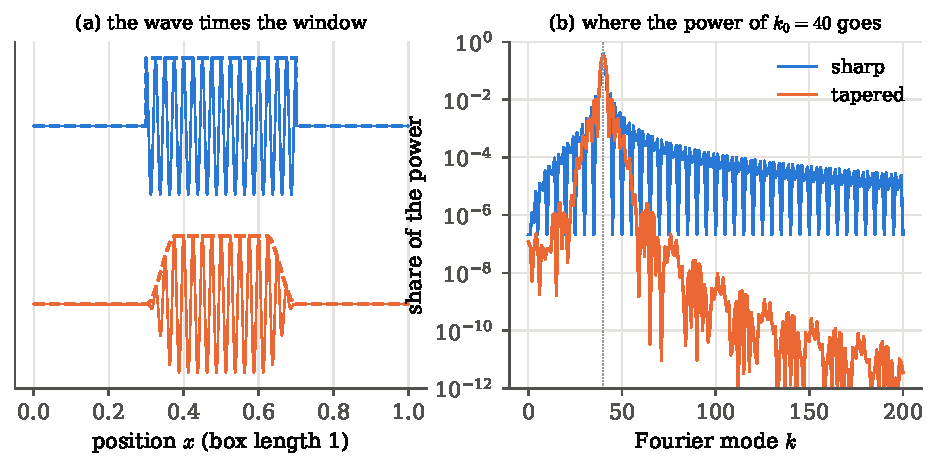
\includegraphics[width=12cm]{figures/ch08/leakage_1d.pdf}
\caption{A single Fourier mode seen through $40\%$ of the box. Left: the wave times a
sharp window (blue) and times a cosine-tapered window (orange), offset for clarity. Right:
the share of the power that lands at each Fourier mode. The sharp window spreads the spike at
$k_0=40$ into a slowly falling comb of side lobes; the tapered one keeps it within a few modes
and then falls by ten more decades.}
\label{8b:fig:leakage}
\end{figure}

Everything that follows on the sphere is this picture with spherical harmonics in place of
plane waves. One difference matters: on the line the window was fixed and the wave was
unique, whereas the sky has $2\ell+1$ modes at each $\ell$ and the window couples each of them
to many others, so the bookkeeping needs the angular-momentum coupling rules of quantum
mechanics. The physics is identical: a mask with sharp edges has a slowly falling spectrum
and leaks power far away; a tapered mask leaks less and uses the sky less efficiently.

\subsection{The window and its moments}
\label{8b:sec:window}

\begin{workdef}[window, mask, sky fraction and moments]
A \newterm{window} $W(\hat{\bm n})$ assigns to each direction $\hat{\bm n}$ a weight between zero and one
\unpack{one where the sky is used at full weight, zero where it is thrown away}. A binary window is
a \newterm{mask} in the narrow sense. Its observed \newterm{sky fraction} $\fsky$ is the fraction of
the sphere where $W\neq0$, and its \newterm{moments} $w_i$ are defined by
\[
  \fsky w_i=\frac1{4\pi}\int_{4\pi}\dd\Omega\,W^i(\hat{\bm n})
  \qquad\text{\srcref{Hivon}{(9)}},
\]
so that $w_i$ is the average of $W^i$ over the observed region and $w_i=1$ for every $i$ when
$W$ is binary. The window's harmonic coefficients and power spectrum are
\[
  w_{\ell m}=\int\dd\Omega\,W(\hat{\bm n})Y^*_{\ell m}(\hat{\bm n}),\qquad
  \mathcal W_\ell=\frac1{2\ell+1}\sum_m|w_{\ell m}|^2
  \qquad\text{\srcref{Hivon}{(10)}}.
\]
\emph{Operationally:} on HEALPix, $\fsky$ is the fraction of pixels with $W>0$, $w_i$ is the mean
of $W^i$ over those pixels, and $\mathcal W_\ell$ is \texttt{anafast} applied to the mask itself.
\end{workdef}

The window's spectrum $\mathcal W_\ell$ will turn out to be the kernel of the mode coupling, the
spherical version of $|\tilde W_q|^2$ in \eqref{8b:eq:tophat-1d}. Two of its values are fixed by
the moments. The monopole is the square of the mean of the window,
\begin{align}
  \mathcal W_0
  &\eqby{1}|w_{00}|^2
   \eqby{2}\Bigl|\frac1{\sqrt{4\pi}}\int\dd\Omega\,W\Bigr|^2
   \eqby{3}\Bigl|\frac{4\pi\fsky w_1}{\sqrt{4\pi}}\Bigr|^2
   =4\pi\fsky^2w_1^2,
  \label{8b:eq:w0}
\end{align}
\begin{explain}
  \item At $\ell=0$ there is one value of $m$, so the average over $m$ is that single term.
  \item $Y_{00}=1/\sqrt{4\pi}$, a constant.
  \item The definition of $w_1$ with $i=1$.
\end{explain}
and the weighted sum of all of them is the total of $W^2$ over the sky:
\begin{align}
  \sum_{\ell\ge0}(2\ell+1)\mathcal W_\ell
  &\eqby{1}\sum_{\ell m}|w_{\ell m}|^2
   \eqby{2}\int\dd\Omega\,W^2(\hat{\bm n})
   \eqby{3}4\pi\fsky w_2 .
  \label{8b:eq:parseval}
\end{align}
\begin{explain}
  \item The definition of $\mathcal W_\ell$, multiplied by $2\ell+1$.
  \item Parseval's theorem on the sphere: expand $W=\sum w_{\ell m}Y_{\ell m}$ in $\int W W^*$ and use
        the orthonormality $\int Y_{\ell m}Y^*_{\ell'm'}=\delta_{\ell\ell'}\delta_{mm'}$ (\cref{7b:sec:ylm}). $W$ is real, so $W^2=|W|^2$.
  \item The definition of $w_2$ with $i=2$.
\end{explain}
These are the two identities quoted after \srcref{Hivon}{(10)}. The first says how much of the
window is a constant offset; the second, how much power it has in total. The second is the one
that will reappear as the white-noise level of a masked map.

\paragraph{Example: the controlled masks.}
To study the effect of sky coverage and of shape separately we use eight windows on
$N_{\rm side}=\EightBnside$ maps (\cref{8b:fig:masks}, script \pyname{21_masks.py}):
the full sky; polar caps keeping $10$, $30$ and $70\%$ of the sky; the $10\%$ cap with a $10^\circ$
cosine taper; a Galactic-like band cut $|b|<20^\circ$ around the equator, binary and with a
$5^\circ$ taper; and $400$ randomly placed holes of radius $1^\circ$, the shape of a
point-source mask. A cap of half-opening $\theta_c$ has area $2\pi(1-\cos\theta_c)$, so a cap
holding a fraction $\fsky$ of the sphere has $\cos\theta_c=1-2\fsky$: $\theta_c=\EightBcapTenDeg^\circ$,
$\EightBcapThirtyDeg^\circ$ and $\EightBcapSeventyDeg^\circ$. The band keeps
$\fsky=1-\sin20^\circ=\EightBfskyBandExact$, and the pixels give $\EightBfskyBandPix$. Each hole
removes $2\pi(1-\cos1^\circ)$ steradians, and $400$ of them would remove
$400\times2\pi(1-\cos1^\circ)/4\pi=\EightBholesNaive$ of the sky if they never touched; the
pixels report $\EightBholesLost$, because a few random holes overlap.

\begin{figure}[htbp]
\centering
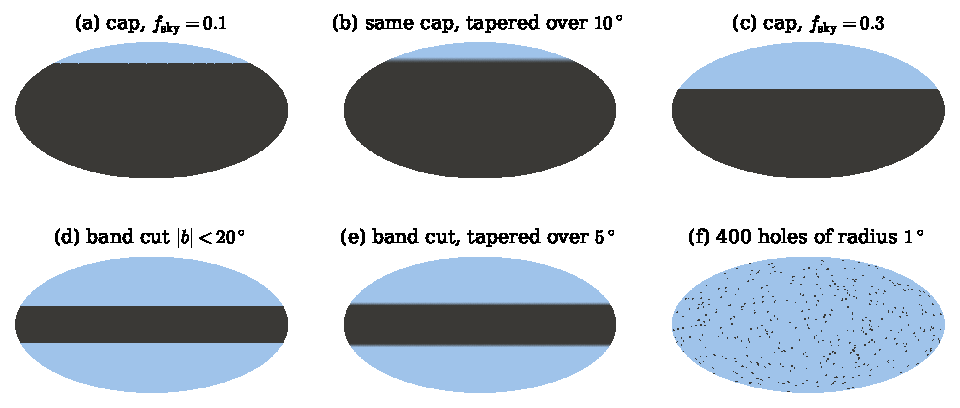
\includegraphics[width=12cm]{figures/ch08/masks.pdf}
\caption{The controlled masks, in Mollweide projection with the north pole at the top. Blue
is the observed sky, dark grey the removed sky. The tapers of (b) and (e) are visible as a
paler rim inside the edge.}
\label{8b:fig:masks}
\end{figure}

\paragraph{Example: the moments of a tapered cap.}
The taper of the $10\%$ cap is $W=\sin^2(\pi d/2\Delta)$ for a distance $d<\Delta=10^\circ$ inside
the edge, and $W=1$ deeper in. How much statistical weight does such a taper cost? The moments need
the averages of $W^2=\sin^4(\pi d/2\Delta)$ and $W^4=\sin^8(\pi d/2\Delta)$ over the cap, and the cap
splits into two parts where these are easy: a core where $W=1$, and a rim where $W$ rises from zero.

\emph{How much of the cap is rim?} The cap's edge is at $\theta_c=36.87^\circ$, where $\cos\theta_c=0.8$, so the cap
has area $2\pi(1-0.8)=1.257$\,sr. The rim runs from $\theta=26.87^\circ$ to $36.87^\circ$ and has area
$2\pi(\cos26.87^\circ-\cos36.87^\circ)=2\pi(0.892-0.800)=0.578$\,sr. That is $0.578/1.257=0.46$ of the cap, and the
core is the remaining $1-0.46=0.54$.

\emph{The average over the rim.} Across the rim the variable $u=\pi d/2\Delta$ runs over a quarter period,
$0\le u\le\pi/2$. If the rim's area were spread evenly in $d$, the rim averages would be the averages of
$\sin^4u$ and $\sin^8u$ over that quarter period. For $\sin^4$ the double-angle identity
$\sin^2u=\tfrac12(1-\cos2u)$ does it:
\begin{align*}
  \langle\sin^4u\rangle
  &\eqby{1}\tfrac14\bigl\langle1-2\cos2u+\cos^22u\bigr\rangle
   \eqby{2}\tfrac14\bigl(1-0+\tfrac12\bigr)=\tfrac38 .
\end{align*}
\begin{explain}
  \item Square $\tfrac12(1-\cos2u)$.
  \item Over $0\le u\le\pi/2$, $2u$ covers half a period of the cosine: $\int_0^{\pi/2}\cos2u\,\dd u=0$, and
        $\cos^22u=\tfrac12(1+\cos4u)$ averages to $\tfrac12$.
\end{explain}
For higher powers, integrating $\int_0^{\pi/2}\sin^ku\,\dd u$ by parts once gives the step
$I_k=\frac{k-1}kI_{k-2}$, so the average of $\sin^{2n}u$ is $\frac{(2n-1)(2n-3)\cdots1}{(2n)(2n-2)\cdots2}$: $\tfrac34\cdot\tfrac12=\tfrac38$
for $n=2$, as above, and $\tfrac78\cdot\tfrac56\cdot\tfrac34\cdot\tfrac12=\tfrac{35}{128}$ for $n=4$. Then
\begin{align*}
  w_2&\approx0.54\times1+0.46\times\tfrac38=0.71,&
  w_4&\approx0.54\times1+0.46\times\tfrac{35}{128}=0.67 .
\end{align*}
The approximation is the even spread of area in $d$. The area of a thin ring is proportional to
$\sin\theta$, which grows from $0.45$ at the inner edge of the rim to $0.60$ at the outer edge, so the
outer part of the rim, where $W$ is small, has about a third more area per degree than the inner part.
The pixel averages, $w_2=\EightBwtwoCapTenApo$ and $w_4=\EightBwfourCapTenApo$, are a little lower than the estimate
for exactly that reason. A
taper this wide changes the effective sky fraction of \srcref{Hivon}{(17)},
$\fsky w_2^2/w_4$, from $0.100$ to $\EightBfeffCapTenApo$: a quarter of the sky's statistical
weight is given up to soften the edge.

\Cref{8b:tab:masks} collects the moments of every mask. For a binary mask all the $w_i$ are one
and only $\fsky$ matters; a taper lowers $w_2$ and $w_4$ and with them the effective sky
fraction. Both identities, \eqref{8b:eq:w0} and \eqref{8b:eq:parseval}, hold for every mask: the
first to within $10^{-15}$ (rounding), the second to within $5\times10^{-4}$, the power the mask
has above the $\ell=767$ at which the sum was stopped.

\begin{table}[htbp]
\centering
\small
\renewcommand{\arraystretch}{1.15}
\begin{tabular}{@{}lccccc@{}}
\toprule
mask & $\fsky$ & $w_2$ & $w_4$ & $w_2^2/w_4$ & $\fsky w_2^2/w_4$ \\
\midrule
cap $0.1$ & $\EightBfskyCapTen$ & $\EightBwtwoCapTen$ & $\EightBwfourCapTen$ & $\EightBweffCapTen$ & $\EightBfeffCapTen$\\
cap $0.1$, $10^\circ$ taper & $\EightBfskyCapTenApo$ & $\EightBwtwoCapTenApo$ & $\EightBwfourCapTenApo$ & $\EightBweffCapTenApo$ & $\EightBfeffCapTenApo$\\
cap $0.3$ & $\EightBfskyCapThirty$ & $\EightBwtwoCapThirty$ & $\EightBwfourCapThirty$ & $\EightBweffCapThirty$ & $\EightBfeffCapThirty$\\
cap $0.7$ & $\EightBfskyCapSeventy$ & $\EightBwtwoCapSeventy$ & $\EightBwfourCapSeventy$ & $\EightBweffCapSeventy$ & $\EightBfeffCapSeventy$\\
band $|b|<20^\circ$ & $\EightBfskyBand$ & $\EightBwtwoBand$ & $\EightBwfourBand$ & $\EightBweffBand$ & $\EightBfeffBand$\\
band, $5^\circ$ taper & $\EightBfskyBandApo$ & $\EightBwtwoBandApo$ & $\EightBwfourBandApo$ & $\EightBweffBandApo$ & $\EightBfeffBandApo$\\
$400$ holes of $1^\circ$ & $\EightBfskyHoles$ & $\EightBwtwoHoles$ & $\EightBwfourHoles$ & $\EightBweffHoles$ & $\EightBfeffHoles$\\
\bottomrule
\end{tabular}
\caption{Sky fraction and moments of the controlled masks at $N_{\rm side}=\EightBnside$.
The last column is the effective sky fraction that enters the mode count of
\srcref{Hivon}{(17)}.}
\label{8b:tab:masks}
\end{table}

\paragraph{The spectrum of a mask.}
The kernel of the leakage is $\mathcal W_\ell$, and its tail decides how far power can travel.
For a cap the tail can be worked out. A cap is symmetric about the pole, so only $m=0$
survives, and with $x=\cos\theta$, $x_c=\cos\theta_c$,
\begin{align}
  w_{\ell0}
  &\eqby{1}2\pi\sqrt{\frac{2\ell+1}{4\pi}}\int_{x_c}^{1}P_\ell(x)\,\dd x
   \eqby{2}2\pi\sqrt{\frac{2\ell+1}{4\pi}}\;
     \frac{P_{\ell-1}(x_c)-P_{\ell+1}(x_c)}{2\ell+1},
  \label{8b:eq:cap-wl}
\end{align}
\begin{explain}
  \item $Y_{\ell0}=\sqrt{(2\ell+1)/4\pi}\,P_\ell(\cos\theta)$, $W=1$ for $\theta<\theta_c$, and the $\phi$
        integral gives $2\pi$.
  \item The Legendre identity $(2\ell+1)P_\ell=P'_{\ell+1}-P'_{\ell-1}$ integrates to
        $\int_{x_c}^1P_\ell\,\dd x=[P_{\ell+1}-P_{\ell-1}]_{x_c}^1/(2\ell+1)$, and $P_\ell(1)=1$ for every $\ell$.
\end{explain}
How fast does this fall at large $\ell$? There the Legendre polynomial is a slowly decaying cosine,
$P_\ell(\cos\theta_c)\approx\sqrt{2/(\pi\ell\sin\theta_c)}\cos[(\ell+\tfrac12)\theta_c-\pi/4]$. Three factors of
\eqref{8b:eq:cap-wl} depend on $\ell$, and they are best counted one at a time.
\begin{align*}
  \sqrt{\frac{2\ell+1}{4\pi}}&\relby{1}{\propto}\ell^{1/2},\\
  P_{\ell-1}(x_c)-P_{\ell+1}(x_c)
  &\eqby{2}\sqrt{\frac2{\pi\ell\sin\theta_c}}\,\bigl[\cos(\varphi-\theta_c)-\cos(\varphi+\theta_c)\bigr]\\
  &\eqby{3}\sqrt{\frac2{\pi\ell\sin\theta_c}}\;2\sin\theta_c\,\sin\varphi\;\propto\;\ell^{-1/2},\\
  \frac1{2\ell+1}&\relby{4}{\propto}\ell^{-1}.
\end{align*}
\begin{explain}
  \item The normalisation of $Y_{\ell0}$ grows as the square root of $\ell$.
  \item The asymptotic form for $\ell\mp1$, with $\varphi\equiv(\ell+\tfrac12)\theta_c-\pi/4$; the amplitudes for
        $\ell-1$ and $\ell+1$ differ from the one at $\ell$ only by a relative $O(1/\ell)$.
  \item $\cos(\varphi-\theta_c)-\cos(\varphi+\theta_c)=2\sin\varphi\sin\theta_c$. The phases of the two
        polynomials differ by $2\theta_c$, which is not small for a cap, so the difference is as large as
        each term: no cancellation.
  \item The factor from the integral.
\end{explain}
The product is $\ell^{1/2}\times\ell^{-1/2}\times\ell^{-1}$, so $w_{\ell0}\propto\ell^{-1}$, oscillating with $\sin\varphi$,
and $\mathcal W_\ell=|w_{\ell0}|^2/(2\ell+1)\propto\ell^{-2}/\ell=\ell^{-3}$. Weighted by the number of modes,
$(2\ell+1)\mathcal W_\ell\propto\ell^{-2}$: the same $1/q^2$ tail as the sharp window on the line.
\Cref{8b:fig:mask-spectra} shows it: the binary cap and band fall by about three decades per
decade of $\ell$, the tapered versions drop by ten decades by $\ell\approx200$ and then sit on the
floor of the numerical precision. The holes behave differently. Each hole is a small disc of
radius $1^\circ$, nearly a point on large scales, and $400$ randomly placed points have a nearly
flat spectrum up to $\ell\sim180^\circ/1^\circ$; their $\mathcal W_\ell$ is small but does not fall. That
will make the holes a poor neighbour for the high-$\ell$ spectrum.

\begin{figure}[htbp]
\centering
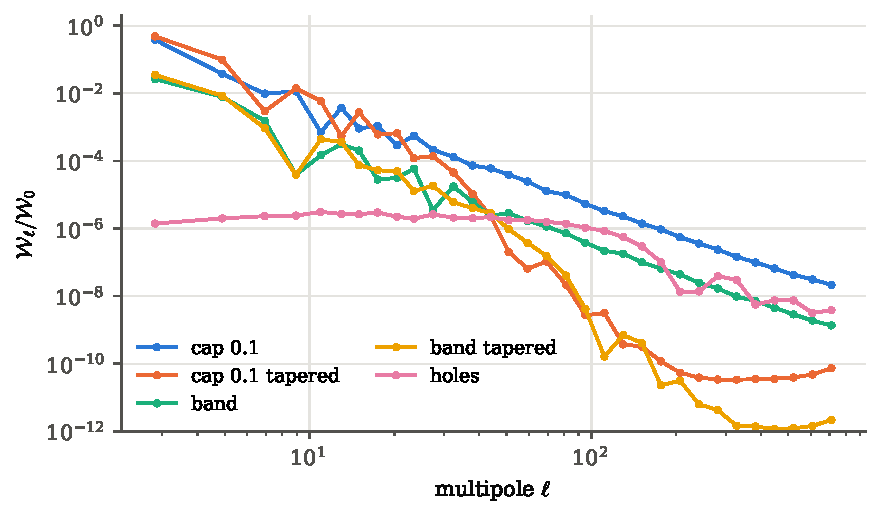
\includegraphics[width=10cm]{figures/ch08/mask_spectra.pdf}
\caption{The power spectra of the masks, normalised to their monopole. The sharp cap and band
fall slowly, about as $\ell^{-3}$; their tapered versions collapse by ten decades and then stop
at the numerical floor. The holes have a low, flat spectrum that stays up to the highest $\ell$.}
\label{8b:fig:mask-spectra}
\end{figure}

\subsection{The pseudo-spectrum}
\label{8b:sec:pseudo}

The quantity we can compute from a masked map is the obvious one: transform the masked map
and average the squared coefficients over $m$. With the masked coefficients
\begin{align}
  \tilde a_{\ell m}
  &=\int\dd\Omega\,\Delta T(\hat{\bm n})W(\hat{\bm n})Y^*_{\ell m}(\hat{\bm n})
   \approx\Omega_{\rm pix}\sum_pW(p)\,\Delta T(p)\,Y^*_{\ell m}(p),
  \label{8b:eq:pseudo-alm}\\
  \widetilde C_\ell&=\frac1{2\ell+1}\sum_{m=-\ell}^{\ell}|\tilde a_{\ell m}|^2,
  \label{8b:eq:pcl}
\end{align}
\srcref{Hivon}{(11)--(13)}, where the sum runs over the pixels $p$ of area $\Omega_{\rm pix}$ and
$\Delta T$ is the observed map of \cref{8a:sec:model}, sky plus noise.
$\widetilde C_\ell$ is the \newterm{pseudo-spectrum} (or pseudo-$\Cell$), and an estimator built on it is a
\newterm{pseudo-$\Cell$ estimator}. The cosmology notes write the same construction as
$\widetilde\Theta=\Theta W$ with the mask expanded in $w_{\ell m}$ (see the cosmology notes).
On the full sky $W=1$ and $\widetilde C_\ell$ is the observed spectrum of \cref{8a:sec:noise-bias}.

Computing \eqref{8b:eq:pseudo-alm} for every $(\ell,m)$ by brute force costs
$N_{\rm pix}\ell_{\max}^2$ operations, but on a grid of iso-latitude rings, like HEALPix, the sum
over $\phi$ along each ring is a fast Fourier transform and the cost drops to
$N_{\rm pix}^{1/2}\ell_{\max}^2$ \srcref{Hivon}{§2.2}. That is the reason the pseudo-spectrum,
and not a likelihood, is the workhorse at high $\ell$: for a Planck map it is a few seconds, where
the exact likelihood of \cref{8a:sec:why-not-ml} needs $N_{\rm pix}^3$ operations. Our
transforms use \texttt{map2alm} with \texttt{iter=0}, which is exactly the pixel sum
\eqref{8b:eq:pseudo-alm}; iterating would try to correct the quadrature error, which is
negligible below $\ell=2N_{\rm side}$ (\cref{7b:sec:healpy}) and is part of what the coupling
calculation of \cref{8b:sec:coupling} has to reproduce anyway.

\begin{keyidea}[A mask is a product in the sky, a convolution in $\ell$]
Multiplying the map by $W$ multiplies nothing in harmonic space; it convolves. Each pseudo-coefficient
$\tilde a_{\ell m}$ is a combination of true coefficients at many $(\ell',m')$, with weights set by
the window's own coefficients $w_{\ell m}$. A sharp edge gives the window a tail $\propto\ell^{-3}$
and moves power far; a smooth edge confines it to neighbouring multipoles.
\end{keyidea}

\paragraph{The code.}
The masks are a few lines each. A cap is a test on the colatitude of each pixel; the taper is
applied to the distance $d$ from the edge, measured inwards:
\pyfile[firstline=29,lastline=56]{code/ch08/lib_masks.py}{Masks and their cosine taper}
\noindent
\pyname{taper} returns $0$ outside the mask, rises as $\sin^2(\pi d/2\Delta)=\frac12[1-\cos(\pi d/\Delta)]$
across a rim of width $\Delta$, and returns $1$ deeper in; with $\Delta=0$ it is the binary mask.
\pyname{cap} converts the requested sky fraction into the half-opening angle with
$\cos\theta_c=1-2\fsky$ and applies the taper to $\theta_c-\theta$. Because the taper eats into the cap
from its edge, the area with $W>0$, and hence $\fsky$, is the same with and without it, and only the
moments change (\cref{8b:tab:masks}).

The simulation itself is the loop of \cref{8a:sec:pipeline} with one extra line. Each of the
$\EightBNsim$ skies is drawn from the fiducial spectrum, smoothed by the $30'$ beam and the pixel window,
and given white noise of $200\,\mu$K\,arcmin (the experiment of \cref{8a:sec:model}); then the same map
is multiplied by each of the eight masks and transformed:
\pyfile[firstline=48,lastline=67]{code/ch08/23_mc_masked.py}{The cut-sky Monte Carlo: one sky, eight masks}
\noindent
\pyname{pcl} is \eqref{8b:eq:pseudo-alm}--\eqref{8b:eq:pcl}. Observing the \emph{same} sky through all
eight masks (line 67) is the common-random-numbers trick of \cref{8a:sec:pipeline}: differences
between masks are then differences of geometry, not of luck. The sky's own full-sky spectrum
(line 64) is stored as well, so that every estimate can also be compared with the spectrum of the
very sky it came from. The run was split into eight chunks of $250$ skies with their own random
streams, so that an interruption costs at most one chunk; it took $\EightBCPUMinutes$ CPU-minutes,
$\EightBSecPerSky$\,s per sky for one synthesis and nine transforms. The full research version of
this loop simulates maps at $N_{\rm side}=2048$ up to $\ell\approx2500$, with the real scan and noise;
ours stops at $N_{\rm side}=\EightBnside$ and $\ell=767$, which keeps the acoustic peaks and the start
of the damping tail and gives up the high-$\ell$ multipoles where the beam has removed the signal
anyway.

\begin{pitfall}[Which sky fraction?]
Three different ``sky fractions'' appear in cut-sky formulas, and they are equal only for a binary
mask. $\fsky$ counts the pixels with $W\neq0$; $\fsky w_2$ is the factor by which a mask lowers
the power of white noise (\cref{8b:sec:coupling}); $\fsky w_2^2/w_4$ counts the effective number of
modes (\cref{8b:sec:distribution}). Using $\fsky$ for a tapered mask overestimates the number of
modes, by a factor $\EightBfskyCapTenApo/\EightBfeffCapTenApo=1.33$ for our tapered cap.
\end{pitfall}
\section{The mode-coupling matrix}
\label{8b:sec:coupling}

On the line, the masked wave's spectrum was the window's spectrum shifted to $k_0$
(\cref{8b:sec:leakage}). On the sphere the pseudo-spectrum $\widetilde C_\ell$ of
\eqref{8b:eq:pcl}, the $m$-average of the squared coefficients of the masked map, is again
fixed on average by the window's spectrum $\mathcal W_\ell$ (\cref{8b:sec:window}) and the true
spectrum $\Cell$. The question is: if the sky has spectrum $\Cell$ and we observe it through a
window $W$, what is $\langle\widetilde C_\ell\rangle$, the average of the pseudo-spectrum over
skies? The answer is a matrix, the \newterm{mode-coupling matrix} $M_{\ell\ell'}$, and the whole
of the MASTER method rests on it.

\subsection{From the window to the coupling kernel}
\label{8b:sec:kernel}

\paragraph{Masked coefficients are linear in the true ones.}
Expand the true sky as $\Delta T=\sum_{\ell'm'}a_{\ell'm'}Y_{\ell'm'}$ inside the integral
\eqref{8b:eq:pseudo-alm}:
\begin{equation}
  \tilde a_{\ell m}=\sum_{\ell'm'}K_{\ell m,\ell'm'}\,a_{\ell'm'},\qquad
  K_{\ell m,\ell'm'}\equiv\int\dd\Omega\;Y^*_{\ell m}(\hat{\bm n})\,W(\hat{\bm n})\,Y_{\ell'm'}(\hat{\bm n})
  \label{8b:eq:K}
\end{equation}
\srcref{Hivon}{(A16)--(A18)}, \cite[eqs~5a--6]{Efstathiou2004}. A physicist will recognise $K$:
it is the matrix element $\langle\ell m|\hat W|\ell'm'\rangle$ of the operator ``multiply by $W$'' in
the basis of angular-momentum eigenstates. A potential $V(\theta,\phi)$ in quantum mechanics
couples the states $|\ell'm'\rangle$ in exactly this way, and the selection rules of atomic
transitions are the selection rules of mode coupling. On the full sky $W=1$, the operator is the
identity, and $K_{\ell m,\ell'm'}=\delta_{\ell\ell'}\delta_{mm'}$. Because $\tilde a_{\ell m}$ is a linear combination of
Gaussian variables it is Gaussian, but the $\tilde a_{\ell m}$ are no longer independent
\srcref{Hivon}{§A.2}. Their covariance takes two moves:
\begin{align}
  \langle\tilde a_{\ell m}\tilde a^*_{\ell''m''}\rangle
  &\eqby{1}\sum_{\ell'm'}\sum_{\ell'''m'''}K_{\ell m,\ell'm'}K^*_{\ell''m'',\ell'''m'''}\,\langle a_{\ell'm'}a^*_{\ell'''m'''}\rangle
   \eqby{2}\sum_{\ell'm'}C_{\ell'}\,K_{\ell m,\ell'm'}K^*_{\ell''m'',\ell'm'} .
  \label{8b:eq:alm-cov}
\end{align}
\begin{explain}
  \item Write both masked coefficients with \eqref{8b:eq:K}, each with its own summation indices. The
        matrix $K$ is fixed by the window, so the average over skies acts only on the true coefficients.
  \item Full-sky isotropy, $\langle a_{\ell'm'}a^*_{\ell'''m'''}\rangle=C_{\ell'}\delta_{\ell'\ell'''}\delta_{m'm'''}$
        (\cref{7b:sec:isotropy}): the Kronecker deltas collapse the second double sum onto the first.
\end{explain}

\paragraph{Three spherical harmonics and the $3j$ symbols.}
To evaluate $K$ we expand the window as well, $W=\sum_{LM}w_{LM}Y_{LM}$, which leaves an
integral of three harmonics. It is the \newterm{Gaunt integral}:
\begin{equation}
  \int\dd\Omega\,Y_{\ell_1m_1}Y_{\ell_2m_2}Y_{\ell_3m_3}
  =\sqrt{\frac{(2\ell_1+1)(2\ell_2+1)(2\ell_3+1)}{4\pi}}
   \begin{pmatrix}\ell_1&\ell_2&\ell_3\\0&0&0\end{pmatrix}
   \begin{pmatrix}\ell_1&\ell_2&\ell_3\\m_1&m_2&m_3\end{pmatrix},
  \label{8b:eq:gaunt}
\end{equation}
with $Y^*_{\ell m}=(-1)^mY_{\ell,-m}$ for the conjugate \srcref{Hivon}{(A20)}. The formula comes from the
quantum theory of angular momentum, where the product of two harmonics is expanded in single
harmonics with Clebsch--Gordan coefficients; we take it from there. Two of its consequences can be
checked by hand, and they are the ones that matter physically. Each harmonic carries a factor
$e^{im_i\phi}$, so the $\phi$ integral of the product is $\int_0^{2\pi}e^{i(m_1+m_2+m_3)\phi}\dd\phi$, which vanishes
unless $m_1+m_2+m_3=0$: the projections are conserved. And $Y_{\ell_1m_1}Y_{\ell_2m_2}$ is a polynomial of
degree $\ell_1+\ell_2$ in the components of $\hat{\bm n}$, so it contains no harmonic above $\ell_1+\ell_2$, and is
orthogonal to $Y_{\ell_3m_3}$ when $\ell_3>\ell_1+\ell_2$; the same argument for each pair says that the three $\ell$'s must form a triangle. The arrays in brackets are
\newterm{Wigner $3j$ symbols} \unpack{the amplitude for three angular momenta $\ell_1,\ell_2,\ell_3$ with
projections $m_1,m_2,m_3$ to add up to zero total angular momentum}, the symmetric form of the
Clebsch--Gordan coefficients of quantum mechanics,
$\begin{pmatrix}j_1&j_2&j_3\\m_1&m_2&m_3\end{pmatrix}=\frac{(-1)^{j_1-j_2-m_3}}{\sqrt{2j_3+1}}\langle j_1m_1\,j_2m_2|j_3\,{-m_3}\rangle$.
Four of their properties do all the work \srcref{Hivon}{(A21)--(A24)}:
\begin{enumerate}
  \item \emph{Triangle rule:} the symbol vanishes unless $|\ell_1-\ell_2|\le\ell_3\le\ell_1+\ell_2$, as for adding
        two angular momenta in quantum mechanics.
  \item \emph{Projections:} it vanishes unless $m_1+m_2+m_3=0$.
  \item \emph{Parity:} with all $m_i=0$ it vanishes when $\ell_1+\ell_2+\ell_3$ is odd (the product of three
        harmonics with $m=0$ is odd under $\hat{\bm n}\to-\hat{\bm n}$ and integrates to zero).
  \item \emph{Orthogonality:}
        \begin{align*}
        \sum_{\ell_3m_3}(2\ell_3+1)\begin{pmatrix}\ell_1&\ell_2&\ell_3\\m_1&m_2&m_3\end{pmatrix}
        \begin{pmatrix}\ell_1&\ell_2&\ell_3\\m'_1&m'_2&m_3\end{pmatrix}&=\delta_{m_1m'_1}\delta_{m_2m'_2},\\
        \sum_{m_1m_2}\begin{pmatrix}\ell_1&\ell_2&\ell_3\\m_1&m_2&m_3\end{pmatrix}
        \begin{pmatrix}\ell_1&\ell_2&\ell'_3\\m_1&m_2&m'_3\end{pmatrix}&=\frac{\delta_{\ell_3\ell'_3}\delta_{m_3m'_3}}{2\ell_3+1},
        \end{align*}
        the second for $\ell_3$ inside the triangle.
\end{enumerate}
Finally, an even permutation of the columns leaves a $3j$ symbol unchanged and an odd one
multiplies it by $(-1)^{\ell_1+\ell_2+\ell_3}$, so its \emph{square} is symmetric in its columns.

\paragraph{The one sum that does the work.}
Before the main calculation, one double sum that it will meet. Fix $\ell$ and $\ell'$, take any numbers
$c_{LM}$, and ask for the total over all projections $m,m'$ of
$\bigl|\sum_{LM}c_{LM}\,(\ell\;L\;\ell';\,{-m}\;M\;m')\bigr|^2$, where $(\ell\;L\;\ell';\,{-m}\;M\;m')$ is the $3j$ symbol with
that top and bottom row. Then
\begin{align}
  \sum_{mm'}\Bigl|\sum_{LM}c_{LM}\begin{pmatrix}\ell&L&\ell'\\-m&M&m'\end{pmatrix}\Bigr|^2
  &\eqby{1}\sum_{LM}\sum_{L'M'}c_{LM}\,c^*_{L'M'}\sum_{mm'}
     \begin{pmatrix}\ell'&\ell&L\\m'&-m&M\end{pmatrix}\begin{pmatrix}\ell'&\ell&L'\\m'&-m&M'\end{pmatrix}
   \nonumber\\
  &\eqby{2}\sum_{LM}\sum_{L'M'}c_{LM}\,c^*_{L'M'}\,\frac{\delta_{LL'}\delta_{MM'}}{2L+1}
   \eqby{3}\sum_{LM}\frac{|c_{LM}|^2}{2L+1} .
  \label{8b:eq:3j-collapse}
\end{align}
\begin{explain}
  \item Write $|z|^2=zz^*$ as a double sum over $(L,M)$ and $(L',M')$; the $3j$ symbols are real, and the
        order of the sums can be exchanged. Move the columns cyclically,
        $(\ell\;L\;\ell')\to(\ell'\;\ell\;L)$, an even permutation that leaves each symbol unchanged.
  \item The second orthogonality relation, with $\ell_1=\ell'$, $\ell_2=\ell$ and the summed projections
        $m_1=m'$, $m_2=-m$ (as $m$ runs from $-\ell$ to $\ell$, so does $-m$); $L$, $M$, $L'$, $M'$ are held fixed, in
        the roles of $\ell_3$, $m_3$, $\ell'_3$, $m'_3$. Terms with $L$ outside the triangle vanish on both sides.
  \item The Kronecker deltas leave only $L'=L$, $M'=M$.
\end{explain}
All the cross terms between different $(L,M)$ have dropped out: the squared modulus of a sum has
become a sum of squared moduli.

\paragraph{The average pseudo-spectrum.}
Now everything is in place. Insert \eqref{8b:eq:K} into \eqref{8b:eq:pcl} and average:
\begin{align}
  \langle\widetilde C_\ell\rangle
  &\eqby{1}\frac1{2\ell+1}\sum_m\sum_{\ell'm'}C_{\ell'}\,|K_{\ell m,\ell'm'}|^2 \nonumber\\
  &\eqby{2}\frac1{2\ell+1}\sum_{\ell'}C_{\ell'}\sum_{mm'}\Bigl|\sum_{LM}w_{LM}(-1)^m
     \sqrt{\tfrac{(2\ell+1)(2L+1)(2\ell'+1)}{4\pi}}
     \begin{pmatrix}\ell&L&\ell'\\0&0&0\end{pmatrix}
     \begin{pmatrix}\ell&L&\ell'\\-m&M&m'\end{pmatrix}\Bigr|^2 \nonumber\\
  &\eqby{3}\sum_{\ell'}C_{\ell'}\frac{2\ell'+1}{4\pi}\sum_{LM}|w_{LM}|^2(2L+1)
     \begin{pmatrix}\ell&L&\ell'\\0&0&0\end{pmatrix}^2\frac1{2L+1} \nonumber\\
  &\eqby{4}\sum_{\ell'}C_{\ell'}\underbrace{\frac{2\ell'+1}{4\pi}\sum_L(2L+1)\,\mathcal W_L
     \begin{pmatrix}\ell&\ell'&L\\0&0&0\end{pmatrix}^2}_{\displaystyle M_{\ell\ell'}} .
  \label{8b:eq:M}
\end{align}
\begin{explain}
  \item $\widetilde C_\ell$ is the $m$-average of $|\tilde a_{\ell m}|^2$; with \eqref{8b:eq:alm-cov} at $\ell''=\ell$,
        $m''=m$, the average of $|\tilde a_{\ell m}|^2$ is $\sum_{\ell'm'}C_{\ell'}|K_{\ell m,\ell'm'}|^2$.
  \item Expand $W$ in $K$ and use the Gaunt integral \eqref{8b:eq:gaunt} with $Y^*_{\ell m}=(-1)^mY_{\ell,-m}$.
  \item The sign $(-1)^m$ does not depend on $(L,M)$ and has modulus one, so it drops out of the squared
        modulus. Take the factor $\sqrt{(2\ell+1)(2\ell'+1)/4\pi}$ out of the square too, and apply
        \eqref{8b:eq:3j-collapse} with $c_{LM}=w_{LM}\sqrt{2L+1}\,(\ell\;L\;\ell';0\;0\;0)$. The $(2\ell+1)$ that
        comes out cancels the prefactor $1/(2\ell+1)$.
  \item $\sum_M|w_{LM}|^2=(2L+1)\mathcal W_L$ by the definition of the window's spectrum, and the
        squared symbol is symmetric in its columns.
\end{explain}
This is \srcref{Hivon}{(A27)--(A31)}, $\langle\widetilde C_\ell\rangle=\sum_{\ell'}M_{\ell\ell'}C_{\ell'}$
\srcref{Hivon}{(14)}, with
\begin{equation}
  M_{\ell\ell'}=\frac{2\ell'+1}{4\pi}\sum_L(2L+1)\,\mathcal W_L\begin{pmatrix}\ell&\ell'&L\\0&0&0\end{pmatrix}^2 .
  \label{8b:eq:Mdef}
\end{equation}
The matrix depends only on the window, through its spectrum, and not on the sky. It is not
symmetric because of the factor $2\ell'+1$; \textcite{Efstathiou2004} writes it as
$M_{\ell\ell'}=(2\ell'+1)\,\Xi(\ell,\ell',\mathcal W)$ and uses the symmetric matrix
$G_{\ell\ell'}=M_{\ell\ell'}/(2\ell'+1)$ \cite[eqs~9--11]{Efstathiou2004}. NaMaster writes the same
expression with $P^{vw}_{L}=(2L+1)\,\mathrm{PCL}_L(v,w)$, the window's spectrum times its mode count,
in place of $(2L+1)\mathcal W_L$ \cite[eq.~12]{Alonso2019}; for two different windows $v$ and $w$
on two maps it uses their cross-spectrum, which reduces to ours when $v=w=W$.

\paragraph{Beam, noise and filtering.}
The beam and the pixel window act on the sky \emph{before} the mask is applied: the
instrument records the smoothed sky, and the mask is applied to the recorded map. The true spectrum
in \eqref{8b:eq:M} is therefore $T_{\ell'}^2C_{\ell'}$, with $T_\ell=B_\ell p_\ell$ of \cref{8a:sec:beam}.
A filter on the timestream or the map, which suppresses some scales, is modelled by a
\newterm{transfer function} $F_\ell$ in the same place. Noise is added before masking too, and
its masked power $\langle\widetilde N_\ell\rangle$ simply adds:

\begin{keyidea}[The master equation of the cut sky]
\[
  \langle\widetilde C_\ell\rangle=\sum_{\ell'}M_{\ell\ell'}\,F_{\ell'}\,T_{\ell'}^2\,\langle C_{\ell'}\rangle
  +\langle\widetilde N_\ell\rangle
  \qquad\text{\srcref{Hivon}{(15)}},
\]
with $M_{\ell\ell'}$ from \eqref{8b:eq:Mdef}. The coupling depends on the window alone; the beam and
filter sit inside the sum, at the true multipole $\ell'$.
\end{keyidea}

\paragraph{Example: the full sky.}
For $W=1$, $w_{00}=\sqrt{4\pi}$ and every other $w_{LM}$ vanishes, so $\mathcal W_0=4\pi$ and
$\mathcal W_{L>0}=0$. Then
\begin{align*}
  M_{\ell\ell'}
  &\eqby{1}\frac{2\ell'+1}{4\pi}\,4\pi\begin{pmatrix}\ell&\ell'&0\\0&0&0\end{pmatrix}^2
   \eqby{2}(2\ell'+1)\frac{\delta_{\ell\ell'}}{2\ell+1}=\delta_{\ell\ell'} .
\end{align*}
\begin{explain}
  \item Only $L=0$ survives the sum in \eqref{8b:eq:Mdef}.
  \item With $\ell_3=0$ the triangle rule forces $\ell=\ell'$, and
        $\begin{pmatrix}\ell&\ell&0\\0&0&0\end{pmatrix}=(-1)^\ell/\sqrt{2\ell+1}$.
\end{explain}
No coupling, as it must be.

\paragraph{Example: white noise through a mask.}
Uniform white noise has the same power $N$ at every multipole. Its masked power is
\begin{align}
  \langle\widetilde N_\ell\rangle
  &\eqby{1}N\sum_{\ell'}M_{\ell\ell'}
   \eqby{2}\frac N{4\pi}\sum_L(2L+1)\mathcal W_L\sum_{\ell'}(2\ell'+1)\begin{pmatrix}\ell&\ell'&L\\0&0&0\end{pmatrix}^2
   \nonumber\\
  &\eqby{3}\frac N{4\pi}\sum_L(2L+1)\mathcal W_L
   \eqby{4}N\fsky w_2 .
  \label{8b:eq:white}
\end{align}
\begin{explain}
  \item The master equation with $C_{\ell'}=N$ for every $\ell'$ and no beam (noise is not smoothed).
  \item Insert \eqref{8b:eq:Mdef} and exchange the sums.
  \item The first orthogonality relation with all projections zero: only $m_3=0$ survives and
        $\sum_{\ell'}(2\ell'+1)(\ell\;\ell'\;L;0\;0\;0)^2=1$.
  \item Parseval for the window, \eqref{8b:eq:parseval}.
\end{explain}
This is \srcref{Hivon}{(A32)}. Masked white noise stays white, at a level lowered by the average
of $W^2$ over the sky: each pixel's noise is multiplied by $W$, so its variance by $W^2$. The same
steps with the roles of $\ell$ and $\ell'$ exchanged give the column rule
$\sum_\ell(2\ell+1)M_{\ell\ell'}=(2\ell'+1)\fsky w_2$: all the power of one true multipole is
redistributed, and its total is lowered by the same factor. These two \emph{sum rules} are the
first test of any coupling code.

\paragraph{Example: the flat-sky limit.}
On a small patch the sphere looks flat and the harmonics become plane waves
\srcref{Hivon}{(A1)--(A15)}. The coupling of two Fourier modes is then simply the window's Fourier
coefficient at their difference, $K_{\bm k_1\bm k_2}=\tilde w(\bm k_2-\bm k_1)$, the two-dimensional
version of \eqref{8b:eq:leak-1d}, and the average power becomes
$\langle\widetilde C_{k_1}\rangle=\int k_2\dd k_2\,M_{k_1k_2}\langle C_{k_2}\rangle$ with
$M_{k_1k_2}=2\pi\int k_3\dd k_3\,\mathcal W(k_3)J(k_1,k_2,k_3)$ \srcref{Hivon}{(A14)}. Here
$J(k_1,k_2,k_3)=\frac2\pi(2k_1^2k_2^2+2k_1^2k_3^2+2k_2^2k_3^2-k_1^4-k_2^4-k_3^4)^{-1/2}$
\srcref{Hivon}{(A10)} is the density of ways in which three vectors of lengths $k_1,k_2,k_3$ can close
into a triangle, $\bm k_1=\bm k_2+\bm k_3$, which is momentum conservation. For large multipoles the
squared $3j$ symbol tends to exactly the same expression in $(\ell_1,\ell_2,\ell_3)$
\srcref{Hivon}{(A26)}: the triangle rule of angular momentum is the triangle of momentum
conservation, and the curved-sky kernel reduces to the flat one.

\subsection{Computing the $3j$ symbols and the matrix}
\label{8b:sec:coupling-code}

Only symbols with all projections zero enter \eqref{8b:eq:Mdef}, and for those there is a
closed form. For even $J=\ell_1+\ell_2+\ell_3$ and $g=J/2$,
\begin{equation}
  \begin{pmatrix}\ell_1&\ell_2&\ell_3\\0&0&0\end{pmatrix}^2
  =\frac{(J-2\ell_1)!\,(J-2\ell_2)!\,(J-2\ell_3)!}{(J+1)!}
   \Biggl[\frac{g!}{(g-\ell_1)!\,(g-\ell_2)!\,(g-\ell_3)!}\Biggr]^2
  \label{8b:eq:3j-closed}
\end{equation}
\srcref{Hivon}{(A25)}, and zero for odd $J$.

\paragraph{Example: one symbol by hand.}
For $(2,2,2)$: $J=6$, $g=3$. The first factor is $2!\,2!\,2!/7!=8/5040$ and the bracket is
$3!/(1!\,1!\,1!)=6$, so the square is $8\times36/5040=2/35=0.057143$. The code returns
$\EightBthreejExample$.

The factorials overflow a double-precision number beyond $170!$, long before $\ell=767$. The
standard cure is to work with logarithms: $\ln n!$ is the log-gamma function
$\ln\Gamma(n+1)$, the logarithm of \eqref{8b:eq:3j-closed} is a sum of eight such terms, and
one exponential at the end gives a number of ordinary size. No recursion is needed for this
family of symbols, and the closed form is exact up to rounding. Checked against the exact
rational values from \texttt{sympy.physics.wigner} for six triples up to $(400,380,30)$, the worst
relative error is $\EightBthreejWorst$, and the orthogonality sum
$\sum_{\ell_3}(2\ell_3+1)(100\;140\;\ell_3;0\;0\;0)^2$ comes out as $\EightBorthSum$.
\pyfile[firstline=137,lastline=170]{code/ch08/lib_masks.py}{The squared $3j$ symbol and the coupling matrix}
\noindent
\pyname{_w3j000_sq} first applies the selection rules (odd $J$, triangle) and returns zero
without computing anything; otherwise it evaluates the logarithm of \eqref{8b:eq:3j-closed}
from a precomputed table \pyname{lf} of $\ln n!$. \pyname{_coupling} is \eqref{8b:eq:Mdef}
literally: for each pair $(\ell,\ell')$ it sums over the multipoles $L$ of the window allowed by the
triangle rule, starting at $|\ell-\ell'|$ and stepping by two to skip the odd-parity terms that
vanish. The loop over rows runs in parallel (\pyname{prange}, compiled by \pyname{numba}).
For $\ell,\ell'\le767$ a matrix takes a few seconds. It needs the window's spectrum up to
$L=\ell+\ell'$, so the masks' spectra were computed to $L=1535$
(script \pyname{22_coupling.py}).

\paragraph{The sum rules, numerically.}
The white-noise rule $\sum_{\ell'}M_{\ell\ell'}=\fsky w_2$ holds for every row $\ell\le400$ to within
$\EightBrowRuleCapTen$ for the sharp $10\%$ cap, $\EightBrowRuleCapTenApo$ for its tapered version and
$\EightBrowRuleHoles$ for the holes; the residue is the part of each row that would lie beyond
$\ell'=767$ and is cut off. Sharp masks have the slowest tails and lose the most.

\subsection{Checking the matrix against the sky}
\label{8b:sec:coupling-check}

A formula with this many indices deserves two independent checks, one without random numbers and
one with them.

\paragraph{A direct check, mode by mode.}
A sky whose power is all in one multipole $\ell'$ is a sum of its $2\ell'+1$ real modes: the real
$Y_{\ell'0}$ with variance $C_{\ell'}$, and the real and imaginary parts of $a_{\ell'm'}$ for $m'>0$,
each with variance $C_{\ell'}/2$ (\cref{7b:sec:dof}). Because the modes are independent, the
average pseudo-spectrum of such a sky is the variance-weighted sum of the pseudo-spectra of
each masked mode. Setting $C_{\ell'}=1$ that sum is the column $M_{\ell\ell'}$ of the matrix, computed
with $2\ell'+1$ map transforms and no $3j$ symbol and no random number. Script
\pyname{24_coupling_check.py} does this for $\ell'=20$ and $100$ through the $10\%$ cap and the band.
The two computations agree to $\EightBdirectWorst$ wherever the column carries power
(\cref{8b:fig:coupling-direct}). This is also the ``Monte Carlo of the mask response'' in its
cheapest form: one transform per mode, nothing random.

\begin{figure}[htbp]
\centering
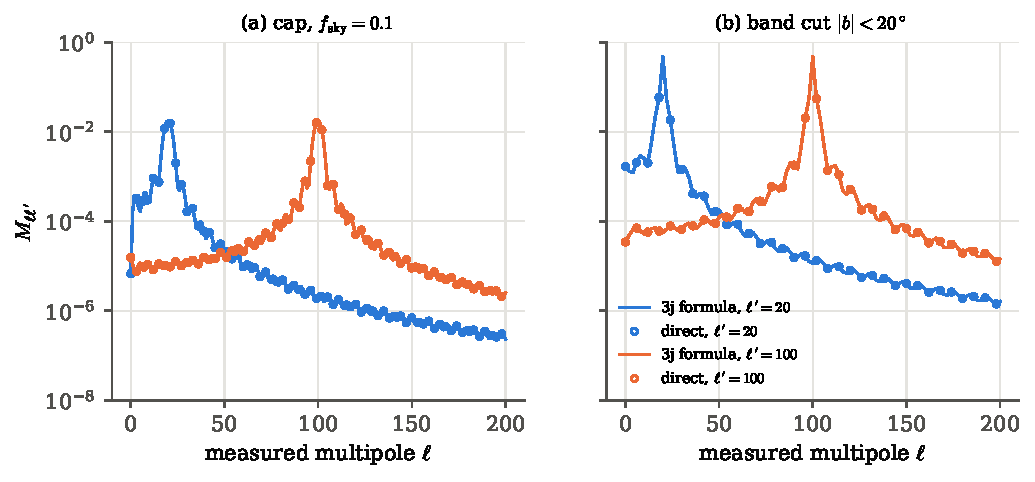
\includegraphics[width=12cm]{figures/ch08/coupling_direct.pdf}
\caption{Two columns of the coupling matrix, $\ell'=20$ (blue) and $\ell'=100$ (orange), from the
$3j$ formula (lines) and from transforming each masked real mode of that multipole (circles).
(a) The $10\%$ cap. (b) The band cut, shown at the multipoles of the same parity as $\ell'$ only:
the band is symmetric about the equator and does not couple multipoles of opposite parity.}
\label{8b:fig:coupling-direct}
\end{figure}

\paragraph{The band and parity.}
The right panel of \cref{8b:fig:coupling-direct} shows a selection rule at work. The band is
symmetric under $\theta\to\pi-\theta$, the reflection through the equator. Its coefficients
$w_{LM}$ are nonzero only for even $L$ (and $M=0$), because $Y_{L0}$ is odd under the reflection
for odd $L$. The parity rule of the $3j$ symbol then requires $\ell+\ell'+L$ even, so $\ell+\ell'$ is
even: the band couples $\ell'$ only to multipoles of the same parity. The caps have no such
symmetry and couple everything.

\paragraph{The Monte Carlo check.}
The second check uses the $\EightBNsim$ simulated skies of \cref{8b:sec:pseudo}, with beam, pixel window
and noise. For each mask we compare the mean of the simulated pseudo-spectra with the master
equation, $\sum_{\ell'}M_{\ell\ell'}T_{\ell'}^2C_{\ell'}+N\fsky w_2$, and divide the difference by the Monte Carlo
error of the mean, the simulated standard deviation over $\sqrt{\EightBNsim}$. If the formula is
right, these pulls are draws of a standard Gaussian, and their mean square over
$2\le\ell\le\EightBLchk$ should be close to one. It is $\EightBpullchiFull$ on the full sky,
$\EightBpullchiCapThirty$ for the $30\%$ cap, $\EightBpullchiBand$ for the band, $\EightBpullchiHoles$ for the holes and
$\EightBpullchiCapTen$ and $\EightBpullchiCapTenApo$ for the sharp and tapered $10\%$ caps
(\cref{8b:fig:mean-check}). The last two are a little below one, and that is expected: through a small
cap neighbouring multipoles are strongly correlated (\cref{8b:sec:distribution}), so the $599$ pulls
contain only about $60$ independent numbers, and their mean square scatters by about
$\sqrt{2/60}\approx0.2$ around one.

\begin{figure}[htbp]
\centering
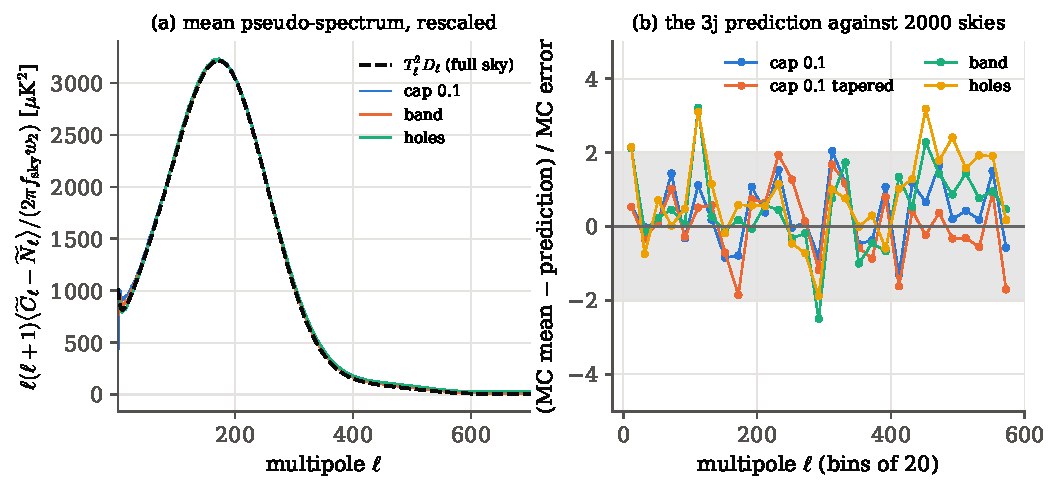
\includegraphics[width=12cm]{figures/ch08/mean_check.pdf}
\caption{The master equation against $\EightBNsim$ simulated skies. (a) The mean pseudo-spectrum
through four masks, noise subtracted and divided by $\fsky w_2$, on the full-sky spectrum (dashed): at
this scale the coupling is invisible except as a smoothing of the curve. (b) The mean minus the
prediction of \eqref{8b:eq:Mdef}, in units of its Monte Carlo error, in bins of $20$ multipoles: the
residuals scatter within $\pm2$ (grey) with no trend.}
\label{8b:fig:mean-check}
\end{figure}

\begin{pitfall}[The coupling needs the window to twice the band limit]
$M_{\ell\ell'}$ involves $\mathcal W_L$ up to $L=\ell+\ell'$. Computing the mask's spectrum only to the
analysis band limit $\ell_{\max}$ silently drops the coupling between the highest multipoles, worst
for sharp masks whose spectra fall slowly. Compute $\mathcal W_L$ to $2\ell_{\max}$, and if the
pixelisation cannot represent the mask that far ($L>3N_{\rm side}$ on HEALPix), compute the mask at
a higher resolution than the data.
\end{pitfall}

\subsection{Leakage and apodisation on the sphere}
\label{8b:sec:apodisation}

\Cref{8b:fig:coupling-columns} shows what happens to the power of a single true multipole,
$\ell'=100$, through each mask: the share $(2\ell+1)M_{\ell,100}/\sum_\ell(2\ell+1)M_{\ell,100}$ that lands at
each measured $\ell$. Every mask keeps most of the power near $\ell'$, in a central peak whose width is
set by the size of the observed region, as for any diffraction pattern: a region of angular size
$\Theta$ cannot resolve multipoles closer than about $\pi/\Theta$. Outside the peak the masks differ
by orders of magnitude, exactly as the one-dimensional windows did. The fraction landing more than
$20$ multipoles away is $\EightBfarLeakCapTen\%$ for the sharp $10\%$ cap and $\EightBfarLeakCapTenApo\%$ for the
tapered one; $\EightBfarLeakBand\%$ for the sharp band and $\EightBfarLeakBandApo\%$ for the tapered one;
$\EightBfarLeakCapThirty\%$ and $\EightBfarLeakCapSeventy\%$ for the $30\%$ and $70\%$ caps; and
$\EightBfarLeakHoles\%$ for the holes, whose flat window spectrum carries power to every multipole.

\begin{figure}[htbp]
\centering
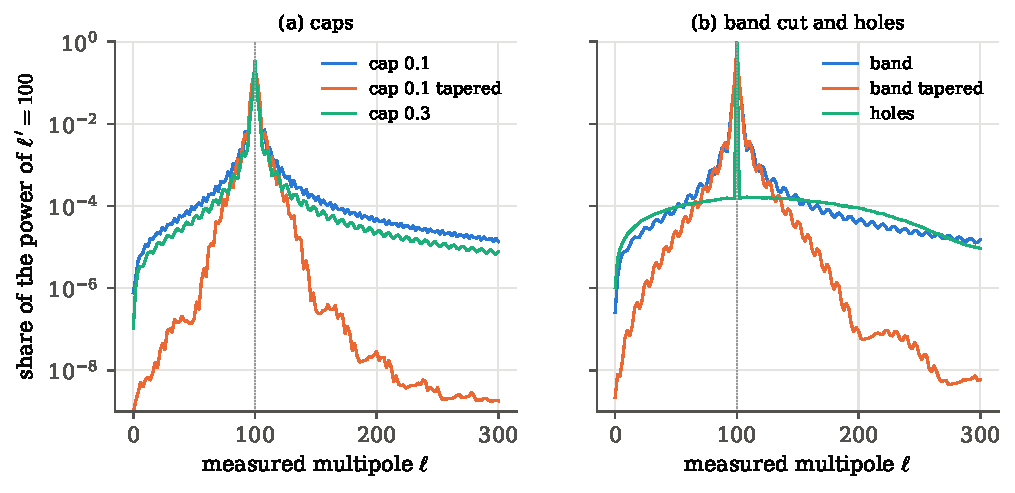
\includegraphics[width=12cm]{figures/ch08/coupling_columns.pdf}
\caption{Where the power of the true multipole $\ell'=100$ goes. (a) Caps: the sharp $10\%$ cap
(blue) and $30\%$ cap (green) leak a slowly falling tail to all $\ell$; the tapered $10\%$ cap
(orange) has a wider central peak but tails eight decades lower. (b) The band cut (blue),
its tapered version (orange), and the holes (green), whose leakage is nearly flat in $\ell$.}
\label{8b:fig:coupling-columns}
\end{figure}

Apodisation therefore buys a clean kernel and pays in two ways. The tapered region uses the sky at
less than full weight, so the effective sky fraction $\fsky w_2^2/w_4$ drops (\cref{8b:tab:masks});
and the observed region is effectively smaller, so the central peak is wider and neighbouring
multipoles become even more correlated. Whether the trade is worth it depends on the spectrum. A
spectrum that falls steeply, like the CMB in its damping tail behind a $30'$ beam, is ruined by a
tail that carries power from the acoustic peaks into multipoles where there is almost none of their
own; there apodisation is indispensable (\cref{8b:sec:naive}). For a nearly flat spectrum leakage
hardly matters, and the sharp mask, which keeps more modes, gives smaller error bars. Hivon et al.\
make the same point for their patch: a well-chosen apodisation can improve the achievable spectral
resolution of a non-convex survey \srcref{Hivon}{§3.1}.

\paragraph{Example: the price of the taper in modes.}
At $\ell=200$ in a bin of $\Delta\ell=20$, the sharp $10\%$ cap offers $(2\ell+1)\Delta\ell\,\fsky=802$ modes by
the counting of \srcref{Hivon}{(17)}; the tapered cap offers
$(2\ell+1)\Delta\ell\,\fsky w_2^2/w_4=401\times20\times\EightBfeffCapTenApo=600$. If the bin were cosmic-variance
limited its error would grow by $\sqrt{802/600}=1.16$. That is the price of the taper; the next
section shows what it buys.
\section{Undoing the mask}
\label{8b:sec:master}

The master equation of \cref{8b:sec:coupling} says what the mask does on average:
$\langle\widetilde C_\ell\rangle=\sum_{\ell'}M_{\ell\ell'}F_{\ell'}T_{\ell'}^2C_{\ell'}+\langle\widetilde N_\ell\rangle$, with
$M_{\ell\ell'}$ the coupling matrix of the window, $T_\ell$ the beam times the pixel window and $F_\ell$
the transfer function of any filter. We observe $\widetilde C_\ell$ and want $\Cell$. Three recipes
suggest themselves, in increasing order of effort. Divide by a single number, the fraction of the
sky that was used. Invert the matrix, multipole by multipole. Or average the multipoles into
bins first and invert a small matrix between bins. We take them one at a time and ask of each
the question that matters for an estimator: is it unbiased, and if not, why not?

\subsection{The naive estimator: divide by the sky fraction}
\label{8b:sec:naive}

The quickest guess is that a mask removes a fraction of the power and nothing else:
\begin{equation}
  \widehat C^{\,\rm naive}_\ell=\frac{\widetilde C_\ell-\langle\widetilde N_\ell\rangle}{\fsky w_2\,T_\ell^2} .
  \label{8b:eq:naive}
\end{equation}
It has a respectable origin. For a flat spectrum it is exact: the row rule
$\sum_{\ell'}M_{\ell\ell'}=\fsky w_2$ of \eqref{8b:eq:white} says that a constant spectrum comes out of
the mask multiplied by $\fsky w_2$ and nothing else. The question is how far a curved spectrum
departs from that. Subtracting the exact average,
\begin{align}
  \langle\widehat C^{\,\rm naive}_\ell\rangle-\Cell
  &\eqby{1}\frac{\sum_{\ell'}M_{\ell\ell'}T_{\ell'}^2C_{\ell'}}{\fsky w_2T_\ell^2}-\Cell
   \eqby{2}\frac{\sum_{\ell'}M_{\ell\ell'}\bigl(S_{\ell'}-S_\ell\bigr)}{\fsky w_2\,T_\ell^2},
   \qquad S_\ell\equiv T_\ell^2\Cell ,
  \label{8b:eq:naive-bias}
\end{align}
\begin{explain}
  \item The master equation with $F=1$; the noise term cancels against the subtraction.
  \item Write $\Cell=S_\ell/T_\ell^2$ and use the row rule to put $S_\ell$ inside the sum as
        $\sum_{\ell'}M_{\ell\ell'}S_\ell/(\fsky w_2)$.
\end{explain}
so the bias is the kernel-weighted difference between the smoothed spectrum $S$ at the true
multipoles $\ell'$ and at the measured one. Two mechanisms make it nonzero, one near $\ell$ and one far
from it.

\emph{Near $\ell$: curvature.} Divide by $\Cell=S_\ell/T_\ell^2$ and call $\kappa_{\ell'}\equiv M_{\ell\ell'}/(\fsky w_2)$ the
kernel; by the row rule its weights add up to one. Where the spectrum is smooth over the kernel,
expand $S_{\ell'}$ around $\ell$:
\begin{align*}
  \frac{\langle\widehat C^{\,\rm naive}_\ell\rangle-\Cell}{\Cell}
  &\eqby{1}\sum_{\ell'}\kappa_{\ell'}\,\frac{S_{\ell'}-S_\ell}{S_\ell}
   \eqby{2}\frac{S'_\ell}{S_\ell}\sum_{\ell'}\kappa_{\ell'}(\ell'-\ell)
    +\frac{S''_\ell}{2S_\ell}\sum_{\ell'}\kappa_{\ell'}(\ell'-\ell)^2
   \eqby{3}\frac12\,\sigma_K^2\,\frac{S''_\ell}{S_\ell} .
\end{align*}
\begin{explain}
  \item \eqref{8b:eq:naive-bias} divided by $\Cell=S_\ell/T_\ell^2$.
  \item Taylor's expansion $S_{\ell'}=S_\ell+(\ell'-\ell)S'_\ell+\tfrac12(\ell'-\ell)^2S''_\ell$, with the derivatives taken
        with respect to $\ell$; the constant term cancels.
  \item For a kernel symmetric about $\ell$ the first moment $\sum\kappa_{\ell'}(\ell'-\ell)$ vanishes (the factor
        $2\ell'+1$ in $M$ makes it slightly asymmetric, by a relative $\sigma_K/\ell$); the second moment is the
        kernel's variance, $\sigma_K^2$.
\end{explain}
At a peak $S''<0$ and the estimate comes out low; in a trough $S''>0$ and it comes out high. The mask
smooths the peaks and fills the troughs.

\emph{Far from $\ell$: leakage.} If a fraction $\varepsilon$ of the kernel's weight sits far away, at multipoles
where $S$ is near its peak value $S_{\rm peak}$, the second piece of the bias is about
$\varepsilon\,S_{\rm peak}/S_\ell$. A tiny $\varepsilon$ is harmless where $S_\ell$ is near the peak, and dominant where $S_\ell$
is a small fraction of it.

\paragraph{Example: why the damping tail is hit hardest.}
Compare the first peak, $\ell=220$, with the damping tail at $\ell=580$, and put a number on
$S_{\rm peak}/S_\ell$. Behind the $30'$ beam ($\sigma_b=12.7'=3.7\times10^{-3}$\,rad, $\sigma_b^2=1.37\times10^{-5}$) the
beam window is $e^{-\ell(\ell+1)\sigma_b^2}$. At $\ell=220$, $\ell(\ell+1)\sigma_b^2=48\,620\times1.37\times10^{-5}=0.67$ and
the window is $e^{-0.67}=0.51$; at $\ell=580$, $336\,980\times1.37\times10^{-5}=4.6$ and the window is
$e^{-4.6}=0.010$. The spectrum itself is $\Cell=2\pi D_\ell/\ell(\ell+1)$ with $D_{220}\approx5700$ and
$D_{580}\approx2000\,\mu{\rm K}^2$, so
\[
  \frac{C_{220}}{C_{580}}=\frac{5700/48\,620}{2000/336\,980}=\frac{0.117}{0.0059}\approx20,
  \qquad
  \frac{S_{220}}{S_{580}}=20\times\frac{0.51}{0.010}\approx1000 .
\]
How much leakage does it take to double the power seen at $\ell=580$? The leaked power must equal
$S_{580}$, which is $10^{-3}$ of the peak. The peak is about a hundred multipoles wide, so each of its
multipoles needs to send only $10^{-3}/100=10^{-5}$ of its power to $\ell=580$. The sharp $10\%$ cap sends
$\EightBfarLeakCapTen\%$ of the power of each multipole more than twenty multipoles away
(\cref{8b:sec:apodisation}). Spread over the several hundred multipoles of the range, that is a few
parts in $10^5$ per multipole: the same size as the threshold. So the far term should be of the order
of the true power at $\ell=580$. That is what the simulations show
(\cref{8b:fig:naive-master}a): the naive estimate through the sharp cap is biased by $\EightBnaiveBiasLowCapTen\%$
in the first bin, rises slowly and reaches $\EightBnaiveBiasMaxCapTen\%$ near $\ell=580$; through the holes
it reaches $\EightBnaiveBiasMaxHoles\%$, and through the sharp band $\EightBnaiveBiasMaxBand\%$. Tapering
cures most of it: $\EightBnaiveBiasMaxCapTenApo\%$ for the tapered cap and $\EightBnaiveBiasMaxBandApo\%$ for the
tapered band at the worst multipole. Even then a few per cent remain, much more than the error of
an average over thousands of skies, so the naive estimator cannot be used for a precision
spectrum.

\begin{figure}[htbp]
\centering
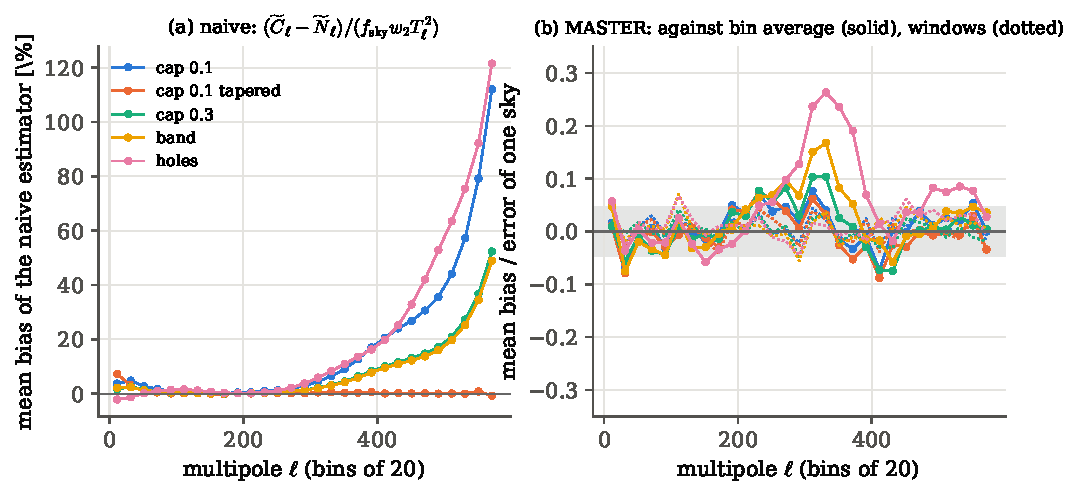
\includegraphics[width=12.5cm]{figures/ch08/naive_master.pdf}
\caption{Bias of the two estimators over $\EightBNsim$ skies, in bins of $20$ multipoles. (a) The naive
estimator \eqref{8b:eq:naive}, in per cent: small at low $\ell$, then rising steeply where the beam has
removed most of the signal and leakage from the acoustic peaks takes over; the tapered cap (orange)
stays within a few per cent. (b) MASTER, as a fraction of the error of a single sky, against the bin
average of the input $D_\ell$ (solid) and against the bandpower-window prediction (dotted). The grey
band is $\pm2$ Monte Carlo errors of the mean.}
\label{8b:fig:naive-master}
\end{figure}

\subsection{Inverting the matrix, multipole by multipole}
\label{8b:sec:invert}

If $M$ is invertible, $\widehat C_\ell=\sum_{\ell'}(M^{-1})_{\ell\ell'}(\widetilde C_{\ell'}-\langle\widetilde N_{\ell'}\rangle)/T_\ell^2$
is unbiased for every spectrum \cite[eq.~12]{Efstathiou2004}. The condition number of $M$ (the ratio
of its largest to its smallest singular value, $2\le\ell,\ell'\le767$) tells us whether that is possible.
It is $\EightBcondFull$ for the full sky, $\EightBcondCapSeventy$ for the $70\%$ cap, $\EightBcondBand$ for the band and
$\EightBcondHoles$ for the holes, all harmless. For the $30\%$ cap it is $\EightBcondCapThirty$ and for the $10\%$
cap $\EightBcondCapTen$: those matrices are singular to machine precision. \Cref{8b:fig:singular} shows the
eigenvalues. For the small caps a fixed fraction of them, $\EightBnullCapTen\%$ and $\EightBnullCapThirty\%$, falls
off a cliff to the rounding floor, while for every other mask none does.

\begin{figure}[htbp]
\centering
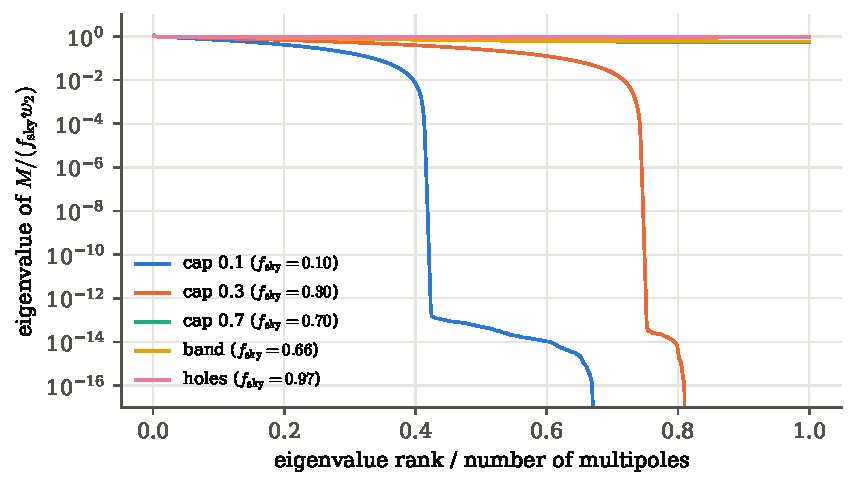
\includegraphics[width=10cm]{figures/ch08/singular.pdf}
\caption{Eigenvalues of the coupling matrix (symmetrised and divided by $\fsky w_2$), sorted and
plotted against their rank as a fraction of the $766$ multipoles. The $10\%$ cap (blue) has a cliff
at $0.41$ and the $30\%$ cap (orange) at $0.74$: beyond it the eigenvalues are pure rounding.
The $70\%$ cap, the band and the holes have no cliff.}
\label{8b:fig:singular}
\end{figure}

\paragraph{The event, and what could have produced it.}
The observed fact is sharp: a fixed fraction of the eigenvalues vanishes, $59\%$ for one cap and
$27\%$ for the other, and none for the band, which removes far more sky than the $70\%$ cap
leaves out. So it is not the amount of sky that matters. The candidates are the shape of the
region, its size, and its smoothness, and the clean way to decide between them is to look at the
coupling from the side of real space.

\emph{What the masked map measures in real space.} Take the masked map $W\Delta T$ and average the product
of its values over all pairs of directions $(\hat{\bm n}_1,\hat{\bm n}_2)$ an angle $\vartheta$ apart, anywhere on the
sphere (where $W=0$ the product is simply zero). Call the result the pseudo-correlation function
$\widetilde C(\vartheta)$. Now average over skies. The window is fixed, so for each pair
$\langle W_1\Delta T_1\,W_2\Delta T_2\rangle=W_1W_2\langle\Delta T_1\Delta T_2\rangle$, and for a statistically isotropic sky
$\langle\Delta T_1\Delta T_2\rangle=C(\vartheta)$ depends only on the separation (\cref{7b:sec:ctheta}). It is the same number
for every pair in the average, so it comes out:
\[
  \langle\widetilde C(\vartheta)\rangle=C(\vartheta)\,\Xi_W(\vartheta),\qquad
  \Xi_W(\vartheta)\equiv\text{average of }W(\hat{\bm n}_1)W(\hat{\bm n}_2)\text{ over pairs a distance }\vartheta\text{ apart}.
\]
The window's pair function $\Xi_W$ is the fraction of pairs at separation $\vartheta$ that the window keeps,
weighted by $W$; on the full sky $\Xi_W=1$, and the masked map measures $C(\vartheta)$ itself.

\emph{The same statement in multipoles.} A pair average of any fixed field $f$ on the sphere has a
Legendre series whose coefficients are the field's spectrum $f_\ell=\sum_m|f_{\ell m}|^2/(2\ell+1)$. With
$x=\hat{\bm n}_1\cdot\hat{\bm n}_2$ and $x_0=\cos\vartheta$,
\begin{align*}
  &\frac{\int\dd\Omega_1\int\dd\Omega_2\,f(\hat{\bm n}_1)f(\hat{\bm n}_2)\,\delta(x-x_0)}{\int\dd\Omega_1\int\dd\Omega_2\,\delta(x-x_0)}\\
  &\qquad\eqby{1}\frac1{8\pi^2}\sum_\ell\frac{2\ell+1}2P_\ell(x_0)\int\dd\Omega_1\int\dd\Omega_2\,f_1f_2\,P_\ell(x)\\
  &\qquad\eqby{2}\frac1{8\pi^2}\sum_\ell\frac{2\ell+1}2P_\ell(x_0)\,\frac{4\pi}{2\ell+1}\sum_m|f_{\ell m}|^2
   \eqby{3}\sum_\ell\frac{2\ell+1}{4\pi}f_\ell\,P_\ell(\cos\vartheta) .
\end{align*}
\begin{explain}
  \item The denominator counts the pairs: $4\pi$ for $\hat{\bm n}_1$ times $2\pi$ for the uniform $\cos$ of the angle
        to $\hat{\bm n}_2$. In the numerator, write the delta function by the completeness of the Legendre polynomials,
        $\delta(x-x_0)=\sum_\ell\frac{2\ell+1}2P_\ell(x)P_\ell(x_0)$.
  \item The addition theorem, $P_\ell(\hat{\bm n}_1\cdot\hat{\bm n}_2)=\frac{4\pi}{2\ell+1}\sum_mY_{\ell m}(\hat{\bm n}_1)Y^*_{\ell m}(\hat{\bm n}_2)$,
        splits the double integral into the product of $\int fY_{\ell m}$ and $\int fY^*_{\ell m}$, which are
        $f^*_{\ell m}$ and $f_{\ell m}$ for a real field.
  \item $\sum_m|f_{\ell m}|^2=(2\ell+1)f_\ell$, and the constants combine as
        $\frac1{8\pi^2}\cdot\frac{2\ell+1}2\cdot\frac{4\pi}{2\ell+1}\cdot(2\ell+1)=\frac{2\ell+1}{4\pi}$.
\end{explain}
With $f=W\Delta T$ and with $f=W$ this gives
\[
  \widetilde C(\vartheta)=\sum_\ell\frac{2\ell+1}{4\pi}\widetilde C_\ell P_\ell(\cos\vartheta),\qquad
  \Xi_W(\vartheta)=\sum_L\frac{2L+1}{4\pi}\mathcal W_LP_L(\cos\vartheta).
\] A product in $\vartheta$ is a convolution in
$\ell$, and the Legendre transform of $\langle\widetilde C(\vartheta)\rangle=C(\vartheta)\Xi_W(\vartheta)$ gives back the coupling
matrix:
\begin{align}
  \langle\widetilde C_\ell\rangle
  &\eqby{1}2\pi\int_{-1}^1\dd x\,P_\ell(x)\,C(x)\,\Xi_W(x)
   \eqby{2}2\pi\sum_{\ell'L}\frac{2\ell'+1}{4\pi}C_{\ell'}\frac{2L+1}{4\pi}\mathcal W_L\int_{-1}^1P_\ell P_{\ell'}P_L\,\dd x
   \nonumber\\
  &\eqby{3}\sum_{\ell'}C_{\ell'}\,\frac{2\ell'+1}{4\pi}\sum_L(2L+1)\mathcal W_L
   \begin{pmatrix}\ell&\ell'&L\\0&0&0\end{pmatrix}^2
   =\sum_{\ell'}M_{\ell\ell'}C_{\ell'} .
  \label{8b:eq:M-real}
\end{align}
\begin{explain}
  \item The inverse Legendre transform, $\Cell=2\pi\int P_\ell(x)C(x)\dd x$ with $x=\cos\vartheta$ (\cref{7b:sec:ctheta}),
        applied to $\widetilde C$, and the product rule.
  \item Expand both $C(x)$ and $\Xi_W(x)$ in Legendre series.
  \item $\int_{-1}^1P_\ell P_{\ell'}P_L\,\dd x=2\begin{pmatrix}\ell&\ell'&L\\0&0&0\end{pmatrix}^2$, the Gaunt integral
        \eqref{8b:eq:gaunt} with all $m=0$ and $Y_{\ell0}=\sqrt{(2\ell+1)/4\pi}\,P_\ell$, integrated over $\phi$.
\end{explain}
The second derivation of \eqref{8b:eq:Mdef} also explains the cliff. Now go through the candidates.
\emph{The cap:} no two points of a cap of half-opening $\theta_c$ are more than $2\theta_c$ apart, so
$\Xi_W(\vartheta)=0$ for $\vartheta>2\theta_c$, and the data say nothing about $C(\vartheta)$ there. Any change of the
$\Cell$ that changes $C(\vartheta)$ only beyond $2\theta_c$ leaves every $\widetilde C_\ell$ untouched, and such changes form
the null space of $M$. How large is it? Count numbers. A spectrum $C_2,\dots,C_{\ell_{\max}}$ is about
$\ell_{\max}$ numbers, and so is the function $C(\vartheta)$ it describes: a Legendre series stopped at $\ell_{\max}$
cannot change on scales finer than about $\pi/\ell_{\max}$ in angle, so it is fixed by about one value per
cell of that width, $\ell_{\max}$ cells across $[0,\pi]$. The data fix $C(\vartheta)$ only in the cells with
$\vartheta<2\theta_c$, about $\ell_{\max}\cdot2\theta_c/\pi$ numbers. The remaining $\ell_{\max}(1-2\theta_c/\pi)$ combinations of the
$\Cell$ change $C(\vartheta)$ only where the window has no pairs; they leave every $\widetilde C_\ell$ unchanged, so
they are directions in which $M$ gives zero. The predicted fraction of zero singular values is
$1-2\theta_c/\pi$. For the $10\%$ cap, $2\theta_c=73.7^\circ$ and the prediction is $59.0\%$; for the
$30\%$ cap, $2\theta_c=132.8^\circ$ and $26.2\%$. The simulations' cliffs are at $\EightBnullCapTen\%$ and
$\EightBnullCapThirty\%$. \emph{The $70\%$ cap} has $2\theta_c=227^\circ>180^\circ$: every separation is observed and
nothing is lost. \emph{The band} removes a great deal of sky but keeps two caps, which contain pairs
at every separation up to antipodal, so $\Xi_W$ never vanishes. \emph{The holes} remove small discs and
leave pairs at every separation.

\begin{keyidea}[When the coupling matrix can be inverted]
$M_{\ell\ell'}$ is invertible exactly when the window contains pairs of directions at every separation
$0\le\vartheta\le\pi$, so that the true correlation function is seen, through $\Xi_W$, at all angles. A
patch of angular diameter $\Theta<\pi$ loses a fraction $1-\Theta/\pi$ of the multipole information
to null modes. Large Galactic cuts are invertible; small patches never are.
\end{keyidea}

This is the content of Efstathiou's rule of thumb, that $M$ remains invertible for Galactic cuts up
to about $30^\circ$ above and below the plane, ``if the two-point correlation function can be
determined on all angular scales from the data within the uncut sky'' \cite[§2.1]{Efstathiou2004}.
He also points out the difference between $M$ and the coupling $K$ of the coefficients themselves:
$K$ is singular for \emph{any} cut, because combinations of $\alm$ that live entirely inside the cut
region leave no trace in the observed sky. The spectrum, a much smaller set of numbers, can be
recovered when the coefficients cannot.

\subsection{Binning first: the MASTER estimator}
\label{8b:sec:binning}

When $M$ cannot be inverted, or when its inverse would amplify noise, the cure is to ask for less.
The counting of \cref{8b:sec:invert} says how much less. A patch of diameter $\Theta$ ($2\theta_c$ for a cap)
fixes $C(\vartheta)$ only for $\vartheta<\Theta$, about $\ell_{\max}\Theta/\pi$ numbers out of $\ell_{\max}$: one number for every
$\pi/\Theta$ multipoles. What the data can determine is therefore not each $\Cell$ but averages of the
spectrum over blocks of about $\delta\ell\sim\pi/\Theta$ multipoles, and the null combinations are the ones that
change sign within such a block, so that the block average does not see them. So we estimate averages
over bins of multipoles, at least $\pi/\Theta$ wide, and assume that the spectrum is constant inside each.

Which spectrum is nearly constant across a bin? Not $\Cell$. On the large-scale plateau $\ell(\ell+1)\Cell$ is
about constant, so $\Cell\propto1/\ell(\ell+1)$: across a bin from $\ell=22$ to $41$, $\Cell$ falls by a factor
$(41\cdot42)/(22\cdot23)=3.4$ while $\ell(\ell+1)\Cell$ stays flat. The quantity to hold constant is therefore the
``flattened'' spectrum $D_\ell=\ell(\ell+1)\Cell/2\pi$ \srcref{Hivon}{§3.4}.

\begin{workdef}[binning operators and the MASTER estimator]
For bins $b$ with edges $\ell^{(b)}_{\rm low}\le\ell<\ell^{(b+1)}_{\rm low}$, the \newterm{binning operator} and its
reciprocal are
\[
  P_{b\ell}=\frac1{2\pi}\frac{\ell(\ell+1)}{\ell^{(b+1)}_{\rm low}-\ell^{(b)}_{\rm low}},\qquad
  Q_{\ell b}=\frac{2\pi}{\ell(\ell+1)}
  \qquad\text{for $\ell$ in bin $b$, zero otherwise}
\]
\srcref{Hivon}{(20)--(21)}: $P$ turns a spectrum $\Cell$ into bin averages of $D_\ell$, and $Q$ turns a
constant $D_b$ back into a $\Cell$ that is flat in $D$ across the bin. The binned coupling and the
\newterm{MASTER estimator} are
\[
  K_{bb'}=P_{b\ell}M_{\ell\ell'}F_{\ell'}T_{\ell'}^2Q_{\ell'b'},\qquad
  \widehat D_b=K^{-1}_{bb'}P_{b'\ell}\bigl(\widetilde C_\ell-\langle\widetilde N_\ell\rangle_{\rm MC}\bigr)
\]
\srcref{Hivon}{(25)--(26)}, with sums over repeated indices. $\langle\widetilde N_\ell\rangle_{\rm MC}$ is the
noise pseudo-spectrum from noise-only simulations, and $\widehat{\mathcal N}_b=K^{-1}_{bb'}P_{b'\ell}\langle\widetilde N_\ell\rangle_{\rm MC}$ is
the \newterm{noise on the sky} \srcref{Hivon}{(27)}.
\end{workdef}

Why the recipe is unbiased, and for what, takes one chain. Start from the master equation and bin it:
\begin{align}
  P_{b\ell}\bigl(\langle\widetilde C_\ell\rangle-\langle\widetilde N_\ell\rangle\bigr)
  &\eqby{1}P_{b\ell}M_{\ell\ell'}F_{\ell'}T^2_{\ell'}C_{\ell'}
   \eqby{2}P_{b\ell}M_{\ell\ell'}F_{\ell'}T^2_{\ell'}Q_{\ell'b'}D_{b'}
   \eqby{3}K_{bb'}D_{b'} ,
  \label{8b:eq:master-derivation}
\end{align}
\begin{explain}
  \item The master equation, multiplied by $P$ (Hivon's (22)--(23)).
  \item \emph{The assumption:} inside each bin $D_\ell$ is a constant $D_{b'}$, so $C_{\ell'}=Q_{\ell'b'}D_{b'}$.
  \item The definition of $K$.
\end{explain}
A square system of $n_{\rm bins}$ equations, which a handful of bins makes small and well
conditioned. Its solution is \srcref{Hivon}{(24)}, and replacing the average by the measurement gives
the estimator. The estimator is linear in the data, so its mean is $K^{-1}P(\langle\widetilde C\rangle-\langle\widetilde N\rangle)$
exactly; step~(2) is the only approximation, and it is a statement about the \emph{sky}, not about
the estimator. For the real spectrum,
\begin{equation}
  \langle\widehat D_b\rangle=\sum_\ell\mathcal F_{b\ell}\Cell,\qquad
  \mathcal F_{b\ell}=\sum_{b'}K^{-1}_{bb'}\sum_{\ell'}P_{b'\ell'}M_{\ell'\ell}F_\ell T_\ell^2 ,
  \label{8b:eq:bpw}
\end{equation}
the \newterm{bandpower window functions} of NaMaster \cite[eqs~18--19]{Alonso2019}. If $D_\ell$ really is
flat in every bin, $\mathcal F_{b\ell}C_\ell$ is the plain bin average; otherwise the two differ by a known,
deterministic amount, and the honest comparison of theory with data passes the theory through
$\mathcal F$.

\paragraph{Example: the full sky.}
With $M=\Id$ and $F=1$, $K_{bb'}$ is diagonal and $K_{bb}=\langle T^2_\ell\rangle_b$, the average of the squared
beam over the bin (the factors $\ell(\ell+1)/2\pi$ of $P$ and $2\pi/\ell(\ell+1)$ of $Q$ cancel). Then
$\widehat D_b=\langle T_\ell^2\widetilde D_\ell\rangle_b/\langle T_\ell^2\rangle_b$: a beam-weighted bin average, not the plain one. Where
$D_\ell$ changes across a bin the two differ. Over $\EightBNsim$ skies the full-sky MASTER mean differs from
the plain bin average by up to $\EightBmasterPullBinFull$ Monte Carlo errors of the mean, but from the
window prediction \eqref{8b:eq:bpw} by at most $\EightBmasterPullWinFull$, which is what thirty Gaussian pulls
give by chance. In units of the error bar of a \emph{single} sky the bin-average offset is
$\EightBmasterBiasSigFull\,\sigma$ at most.

\paragraph{The cut-sky results.}
We ran MASTER with bins of $20$ from $\ell=2$ on every mask, with the noise on the sky subtracted
(\cref{8b:fig:naive-master}b, script \pyname{25_master.py}). Against the bandpower windows the
mean over $\EightBNsim$ skies agrees to within $\EightBmasterPullWinCapTen$ Monte Carlo errors for the $10\%$ cap,
$\EightBmasterPullWinCapThirty$ for the $30\%$ cap, $\EightBmasterPullWinBand$ for the band and $\EightBmasterPullWinHoles$ for the holes,
in the worst of the thirty bins below $\ell=\EightBLrep$: MASTER is unbiased. Against the plain bin
average the largest offset is $\EightBmasterBiasSigCapTen\,\sigma$ (sharp $10\%$ cap), $\EightBmasterBiasSigBand\,\sigma$ (band) and
$\EightBmasterBiasSigHoles\,\sigma$ (holes) of a single sky, a fraction of the error bar that a single
measurement would not notice, but which a likelihood built on the plain bin average would turn
into a systematic shift. The same recipe works for the singular $10\%$ cap. Its diameter is
$2\theta_c=73.7^\circ=1.29$\,rad, so the data fix one number per $\pi/1.29\approx2.4$ multipoles. A bin of $20$
multipoles averages over about eight such blocks; every null combination changes sign within a block
and averages to nearly zero across the bin, so it drops out of the binned equations, and $K_{bb'}$ is
invertible: its condition number is $\EightBcondKCapTen$, against $\EightBcondCapTen$ for $M$, and close to the full sky's $\EightBcondKFull$, which comes from the beam and the pixel window alone.

\begin{pitfall}[Compare theory through the bandpower windows]
A MASTER bandpower is an average of $\Cell$ with weights $\mathcal F_{b\ell}$, not the plain bin average of
$D_\ell$. Comparing data with the binned theory $P_{b\ell}\Cell$ introduces a bias that grows with the
curvature of the spectrum across the bin and with the number of simulations used to test it.
Binning should be chosen after the simulations are done \srcref{Hivon}{§3.4}, and the theory compared
through \eqref{8b:eq:bpw}.
\end{pitfall}

\subsection{A filter on the map: the transfer function}
\label{8b:sec:transfer}

Real data are filtered before the spectrum is taken. Timestreams are high-pass filtered to
suppress the $1/f$ drift of the detectors, signals synchronous with the scan are removed, and the
largest scales, poorly constrained by a small survey and liable to contaminate everything else, are
cut away \srcref{Hivon}{§3.2}. A filter acts along the scan direction and therefore breaks isotropy:
its effect on the spectrum is not a function of $\ell$ alone, and writing it as a transfer function
$F_\ell$ in the master equation is an ansatz to be tested. Hivon et al.\ measure it by simulation.
They run $N^{(\rm s)}_{\rm MC}$ noise-free skies of a known spectrum $C^{\rm th}_\ell$ through the full
filtered observation, average their pseudo-spectra, and solve the master equation for $F$:
\[
  \langle\widetilde C_\ell\rangle_{\rm MC}=\sum_{\ell'}M_{\ell\ell'}F_{\ell'}T^2_{\ell'}C^{\rm th}_{\ell'} .
\]
\emph{A first guess.} If $F_{\ell'}T^2_{\ell'}C^{\rm th}_{\ell'}$ hardly changes across the kernel, it can be taken out of
the sum at $\ell'=\ell$, and the row rule $\sum_{\ell'}M_{\ell\ell'}=\fsky w_2$ leaves
$\langle\widetilde C_\ell\rangle_{\rm MC}\approx\fsky w_2F_\ell T^2_\ell C^{\rm th}_\ell$, so
$F^{(0)}_\ell=\langle\widetilde C_\ell\rangle_{\rm MC}/(\fsky w_2T^2_\ell C^{\rm th}_\ell)$. This is the naive estimator of
\cref{8b:sec:naive} applied to the filter, and it inherits its bias wherever the spectrum is curved.

\emph{A correction.} Write the true transfer function as the guess plus a correction, $F=F^{(0)}+\delta F$, and
insert it into the master equation:
\begin{align*}
  \langle\widetilde C_\ell\rangle_{\rm MC}
  &\eqby{1}\sum_{\ell'}M_{\ell\ell'}F^{(0)}_{\ell'}T^2_{\ell'}C^{\rm th}_{\ell'}+\sum_{\ell'}M_{\ell\ell'}\,\delta F_{\ell'}T^2_{\ell'}C^{\rm th}_{\ell'}
   \relby{2}{\approx}\sum_{\ell'}M_{\ell\ell'}F^{(0)}_{\ell'}T^2_{\ell'}C^{\rm th}_{\ell'}+\fsky w_2\,\delta F_\ell T^2_\ell C^{\rm th}_\ell ,
\end{align*}
\begin{explain}
  \item The master equation is linear in $F$.
  \item The first-guess approximation, now applied only to the correction: if $\delta F_{\ell'}T^2_{\ell'}C^{\rm th}_{\ell'}$
        varies slowly across the kernel, the row rule turns its sum into $\fsky w_2$ times its value at $\ell$.
\end{explain}
Solving for $\delta F_\ell$, and replacing the simulated average by a running average $S$ over about $50$
multipoles to smooth its Monte Carlo noise,
\begin{equation}
  F_\ell=F^{(0)}_\ell+\frac{S\bigl(\langle\widetilde C_\ell\rangle_{\rm MC}\bigr)-\sum_{\ell'}M_{\ell\ell'}F^{(0)}_{\ell'}T^2_{\ell'}C^{\rm th}_{\ell'}}
  {T^2_\ell C^{\rm th}_\ell\fsky w_2}
  \label{8b:eq:F-iter}
\end{equation}
\srcref{Hivon}{(18)}. The exact coupled term now carries the curvature of the spectrum, and only the
correction is treated approximately; one such step was enough for their patch. The step relies on
$\delta F$ being smooth. Where $F^{(0)}$ has inherited a large leakage bias with the shape of the acoustic
peaks, $\delta F$ has that shape too, and the step can overshoot (we meet this below).

\emph{How well $F$ is known.} $F_\ell$ is, up to fixed factors, the average of $N^{(\rm s)}_{\rm MC}$ independent simulated
pseudo-spectra, smoothed over about $\Delta\ell$ multipoles. Each pseudo-spectrum, so smoothed, carries about
$\nu=(2\ell+1)\Delta\ell\fsky$ modes and has a relative variance $2/\nu$ (\cref{8a:sec:knox}); an average of
$N^{(\rm s)}_{\rm MC}$ of them divides that by $N^{(\rm s)}_{\rm MC}$. So
$\delta F_\ell/F_\ell\approx\sqrt{2/[(2\ell+1)\Delta\ell\fsky]}/\sqrt{N^{(\rm s)}_{\rm MC}}$ \srcref{Hivon}{(16), (19)}. They also showed that $F$ barely depends on the assumed spectrum: for a flat and
an open universe, whose first peaks are at $\ell\approx220$ and $420$, the two transfer functions differ by
less than $1\%$ for $50<\ell<1000$ \srcref{Hivon}{Fig.~2}.

\paragraph{Example: a ring filter on the $10\%$ cap.}
Our toy filter imitates destriping: on each ring of constant latitude inside the $10\%$ cap, subtract
the mean of the observed pixels (\pyname{ring_filter} in \pyname{23_mc_masked.py}). It removes,
ring by ring, the pattern a scan along that ring cannot distinguish from a detector offset, and with
it most of the largest-scale power. The first $\EightBNF$ signal-only skies calibrate $F$; the other
$\EightBNtest$ skies, with noise, test it (\cref{8b:fig:transfer}). Two observations stand out.

The ratio $F^{(0)}$ is a poor starting point: at $300\le\ell\le600$ its median is $\EightBFzeroHigh$, larger
than one, because it inherits the leakage bias of the naive estimator, and one step of
\eqref{8b:eq:F-iter} brings it only to $\EightBFoneHigh$ and oscillates wildly at low $\ell$. For the sharp cap,
the running average $S$ and the coupled guess do not cancel: the iteration converges only if
$F^{(0)}$ is already close. The robust alternative uses the binning of MASTER for $F$ as well: take $F$
constant in each bin, $F_\ell=R_{\ell b}F_b$ with $R_{\ell b}=1$ in bin $b$, and solve the small linear system
$P_{b\ell}M_{\ell\ell'}T^2_{\ell'}C^{\rm th}_{\ell'}R_{\ell'b'}F_{b'}=P_{b\ell}\langle\widetilde C_\ell\rangle_{\rm MC}$ directly. It gives
$F_b=\EightBFbinOne$ in the first bin ($2\le\ell<22$), $\EightBFbinTwo$ in the second, $\EightBFbinFive$ in the fifth and
$\EightBFbinHigh$ at high $\ell$: the filter takes out large scales only, as it should.

With this $F$, MASTER on the independent test skies is unbiased again: in the first bin the error is
$\EightBfiltWithLow\%$, against $\EightBfiltWithoutLow\%$ if the filter is ignored ($\EightBfiltWithoutTwo\%$ in the second),
and the largest offset from the bin average is $\EightBfiltWithBiasSig$ of a single sky's error bar.
How well do $\EightBNF$ skies know $F$? Solve for $F_b$ separately in $\EightBdFgroups$ disjoint groups of
$\EightBNF$ skies. Above $\ell=100$ their scatter is $\EightBdFratio\pm\EightBdFratioErr$ times the prediction
\srcref{Hivon}{(19)}: through a cap this small, deconvolution correlates the bins and the counting
formula is optimistic, but even so $\EightBNF$ skies pin $F$ down to well under a per cent above
$\ell\approx100$.

\begin{figure}[htbp]
\centering
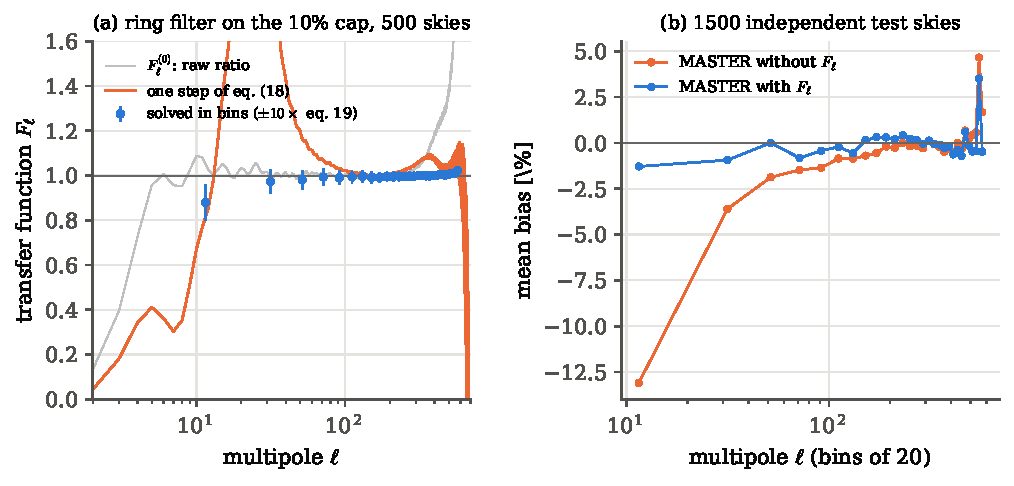
\includegraphics[width=12.5cm]{figures/ch08/transfer.pdf}
\caption{The transfer function of the ring filter on the $10\%$ cap. (a) The raw ratio $F^{(0)}$
(grey), one step of \eqref{8b:eq:F-iter} (orange) and the solution in bins (blue, error bars ten times
the prediction of \srcref{Hivon}{(19)}). (b) MASTER on $\EightBNtest$ test skies, mean bias in
per cent, without $F$ (orange) and with it (blue): ignoring the filter loses $13\%$ of the power in
the first bin.}
\label{8b:fig:transfer}
\end{figure}

A full analysis measures $F$ with end-to-end simulations: the sky is turned into timestreams with
the real pointing, filtered exactly as the data, and made into maps by the same map-maker. That is
what Hivon et al.\ did for Boomerang, and its cost, about half a CPU-day for $300$ simulations on the
computers of 2001 \srcref{Hivon}{(33)}, is why our version filters the maps instead of timestreams.
The reduction keeps the logic (simulate, average, solve for $F$, test on independent skies) and
loses the realism of the scan: our $F$ describes a toy filter, not an instrument.
\section{The scatter of a cut-sky spectrum}
\label{8b:sec:distribution}

MASTER (\cref{8b:sec:binning}) gives an unbiased estimate. A likelihood needs much more than a
mean: the width of the scatter of every estimate, the correlations between estimates at
different multipoles, and the shape of the distribution. On the full sky all three had exact
answers (\cref{7b:sec:mc,8a:sec:shape}): $(2\ell+1)\Chat/\Cell$ is $\chi^2_{2\ell+1}$, the variance is
$2\Cell^2/(2\ell+1)$ plus noise, and different multipoles are independent. A mask breaks all three, and
for a general mask none has a closed form. The $\EightBNsim$ simulated skies of \cref{8b:sec:pseudo}
are now the instrument, and the formulas are what is being tested.

\subsection{The shape of the distribution}
\label{8b:sec:shape-cut}

\paragraph{What the simulations show.}
\Cref{8b:fig:cl-histograms} shows the distribution of the pseudo-spectrum, divided by its mean, at
$\ell=2$, $10$ and $50$, on the full sky and through the $30\%$ and $10\%$ caps. At $\ell=50$ every panel
is a narrow, nearly symmetric bump. At $\ell=2$ the distributions are lopsided: a peak well below the
mean and a long tail to large values. Through the $10\%$ cap the quadrupole's most probable value is
close to zero. The fraction of skies that fall below their own mean, $\frac12$ for a symmetric law, is
$\EightBbelowFullTwo$ on the full sky at $\ell=2$, $\EightBbelowCapThirtyTwo$ through the $30\%$ cap and
$\EightBbelowCapTenTwo$ through the $10\%$ cap: a typical sky shows less large-scale power than the theory
predicts on average, and the smaller the patch, the more so.

\begin{figure}[htbp]
\centering
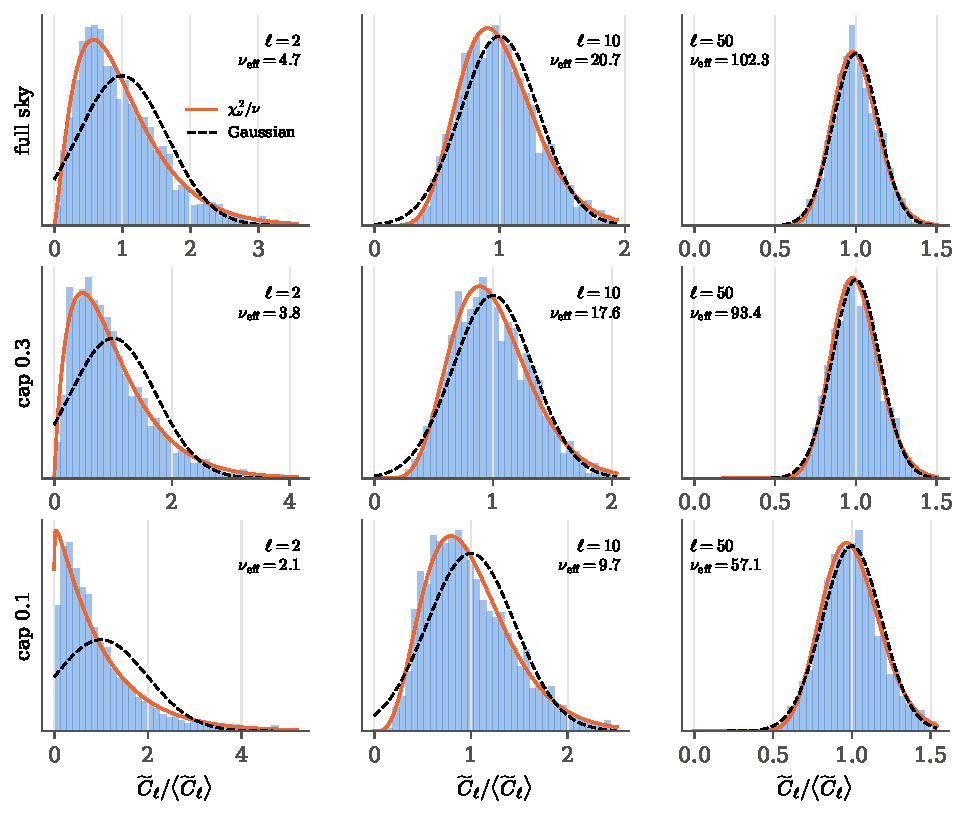
\includegraphics[width=10.5cm]{figures/ch08/cl_histograms.pdf}
\caption{Histograms of $\widetilde C_\ell/\langle\widetilde C_\ell\rangle$ over $\EightBNsim$ skies, at $\ell=2$, $10$ and $50$
(columns) for the full sky and the $30\%$ and $10\%$ caps (rows). Orange: a $\chi^2_\nu/\nu$ with $\nu=\nu_{\rm eff}$
fixed by the simulated mean and variance; dashed: the Gaussian of the same mean and variance. The
white line marks the mean.}
\label{8b:fig:cl-histograms}
\end{figure}

\paragraph{What could have produced that shape?}
Two candidates come to mind. The first is the central limit theorem: $\widetilde C_\ell$ is a sum of
$2\ell+1$ squared coefficients, so perhaps it is Gaussian. The histograms rule this out at low $\ell$, and
the reason is that the sum has few terms. The second is the full-sky law with fewer degrees of
freedom: a scaled $\chi^2_\nu$ with $\nu$ the number of independent modes the patch supplies. That
candidate has a precise justification. The masked coefficients are jointly Gaussian with the
covariance \eqref{8b:eq:alm-cov}, and $\widetilde C_\ell$ is a quadratic form in them.

\emph{The real numbers inside one pseudo-multipole.} The masked map is real, so $\tilde a_{\ell,-m}=(-1)^m\tilde a^*_{\ell m}$:
the coefficients with negative $m$ repeat those with positive $m$, and $\tilde a_{\ell0}$ is real. Collect
the independent real numbers as in \cref{7b:sec:dof}: $z_0=\tilde a_{\ell0}$, and for each $m=1,\dots,\ell$ the two
numbers $\sqrt2\,\mathrm{Re}\,\tilde a_{\ell m}$ and $\sqrt2\,\mathrm{Im}\,\tilde a_{\ell m}$. That is $1+2\ell$ real numbers, a vector $\bm z$.
Then
\[
  (2\ell+1)\widetilde C_\ell=\sum_{m=-\ell}^{\ell}|\tilde a_{\ell m}|^2=\tilde a_{\ell0}^2+2\sum_{m=1}^{\ell}\bigl[(\mathrm{Re}\,\tilde a_{\ell m})^2+(\mathrm{Im}\,\tilde a_{\ell m})^2\bigr]
  =\bm z\T\bm z ,
\]
because $|\tilde a_{\ell,-m}|=|\tilde a_{\ell m}|$ counts each positive $m$ twice; the factors $\sqrt2$ give every
component of $\bm z$ the same weight one. The covariance $\Sigma$ of $\bm z$ follows from \eqref{8b:eq:alm-cov}
and the reality condition, by taking real and imaginary parts. Then
\begin{align}
  (2\ell+1)\widetilde C_\ell
  &\eqby{1}\bm u\T\Sigma\,\bm u
   \eqby{2}\bm u\T O\Lambda O\T\bm u
   \eqby{3}\sum_k\lambda_k\,v_k^2,
  \qquad v_k\iid\Normal(0,1),
  \label{8b:eq:quadform}
\end{align}
\begin{explain}
  \item Write $\bm z=\Sigma^{1/2}\bm u$ with $\bm u$ a vector of independent standard Gaussians; then
        $\bm z\T\bm z=\bm u\T\Sigma\bm u$.
  \item Diagonalise the symmetric matrix $\Sigma=O\Lambda O\T$ with $O$ orthogonal and
        $\Lambda=\diag(\lambda_k)$.
  \item $\bm v=O\T\bm u$ is again a vector of independent standard Gaussians, because an orthogonal
        rotation preserves the identity covariance.
\end{explain}
A cut-sky pseudo-multipole is a weighted sum of independent $\chi^2_1$ variables, with weights equal
to the eigenvalues of the covariance of its own coefficients. On the full sky all the weights are
equal to $\Cell$ and the sum is $\Cell\chi^2_{2\ell+1}$. Through a mask the weights spread out.

\emph{Which $\chi^2$ looks most like it?} Try the model $Y=c\,\chi^2_\nu/\nu$, a scaled $\chi^2$ with two free numbers, $c$
and $\nu$, and choose them so that $Y$ has the same mean and variance as $X\equiv(2\ell+1)\widetilde C_\ell=\sum_k\lambda_kv_k^2$:
\begin{align}
  \langle Y\rangle&\eqby{1}c=\sum_k\lambda_k=\langle X\rangle,&
  \Var Y&\eqby{2}\frac{c^2}{\nu^2}\,2\nu=\frac{2c^2}\nu=2\sum_k\lambda_k^2=\Var X,
  \nonumber\\
  \Longrightarrow\quad
  \nu_{\rm eff}&\eqby{3}\frac{2\langle X\rangle^2}{\Var X}
  =\frac{2\langle\widetilde C_\ell\rangle^2}{\Var\widetilde C_\ell}
  =\frac{\bigl(\sum_k\lambda_k\bigr)^2}{\sum_k\lambda_k^2}\relby{4}{\le}2\ell+1 .
  \label{8b:eq:nu-eff}
\end{align}
\begin{explain}
  \item A $\chi^2_\nu$ has mean $\nu$; each $v_k^2$ is a $\chi^2_1$ with mean one.
  \item A $\chi^2_\nu$ has variance $2\nu$, and a constant factor comes out squared; the $v_k^2$ are independent,
        so their variances $2\lambda_k^2$ add.
  \item Solve the second equation for $\nu$ and insert $c=\langle X\rangle$. The factor $2\ell+1$ cancels in the ratio.
  \item The Cauchy--Schwarz inequality for the vectors $(1,\dots,1)$ and $(\lambda_1,\dots,\lambda_{2\ell+1})$:
        $\bigl(\sum_k1\cdot\lambda_k\bigr)^2\le\bigl(\sum_k1^2\bigr)\bigl(\sum_k\lambda_k^2\bigr)=(2\ell+1)\sum_k\lambda_k^2$, with equality only
        when the two vectors are parallel, that is, when all the weights are equal.
\end{explain}
A few large weights and many small ones make $\nu_{\rm eff}$ small. This moment-matched $\chi^2$ is the
Welch--Satterthwaite approximation; it is exact in its first two moments and approximate beyond.

\emph{The third moment as a test.} Cumulants of independent terms add, and a constant factor $\lambda$
multiplies the third cumulant by $\lambda^3$. A $\chi^2_1$ has variance $2$ and third cumulant $8$
(\cref{8a:sec:shape}), so $\lambda_kv_k^2$ contributes $2\lambda_k^2$ and $8\lambda_k^3$. The skewness, third cumulant over
variance to the power $3/2$, is
\[
  \frac{8\sum_k\lambda_k^3}{\bigl(2\sum_k\lambda_k^2\bigr)^{3/2}}=\frac{\sqrt8\sum_k\lambda_k^3}{\bigl(\sum_k\lambda_k^2\bigr)^{3/2}}
  \qquad\text{against}\qquad\sqrt{\frac8{\nu_{\rm eff}}}\quad\text{for the model.}
\]
With $n$ equal weights the left side is $\sqrt8\,n\lambda^3/(n\lambda^2)^{3/2}=\sqrt{8/n}$ and the two agree exactly; they
stay close as long as the weights are not too unequal.

\emph{The mode count for a smooth spectrum.} Hivon et al.'s count can be recovered from
\eqref{8b:eq:nu-eff} with one picture of the modes. At high $\ell$ a mode of multipole $\ell$ is a short
wave, and the window acts on it locally: a mode concentrated near direction $\hat{\bm n}$ is multiplied by
$W(\hat{\bm n})$, and its variance by $W(\hat{\bm n})^2$. If the spectrum is smooth, so that it does not matter which
neighbouring multipole the mode came from, the $2\ell+1$ eigenvalues are $\lambda_k\approx\Cell W(\hat{\bm n}_k)^2$, with the
$2\ell+1$ directions $\hat{\bm n}_k$ spread evenly over the sphere. Sums over $k$ then become sky averages, which
are the moments of the workdef in \cref{8b:sec:window}:
\begin{align}
  \sum_k\lambda_k&\eqby{1}(2\ell+1)\,\Cell\,\frac1{4\pi}\int\dd\Omega\,W^2=(2\ell+1)\Cell\fsky w_2,&
  \sum_k\lambda_k^2&\eqby{2}(2\ell+1)\,\Cell^2\fsky w_4,
  \nonumber\\
  \nu_{\rm eff}&\eqby{3}\frac{(2\ell+1)^2\Cell^2\fsky^2w_2^2}{(2\ell+1)\Cell^2\fsky w_4}=(2\ell+1)\,\fsky\,\frac{w_2^2}{w_4} .
  \label{8b:eq:hivon-count}
\end{align}
\begin{explain}
  \item An average over evenly spread directions is the sky average; $\frac1{4\pi}\int W^2=\fsky w_2$ by the
        definition of the moments.
  \item The same with $\lambda_k^2\propto W^4$.
  \item \eqref{8b:eq:nu-eff}.
\end{explain}
For a bin of $\Delta\ell$ multipoles, treated as independent, the count is multiplied by $\Delta\ell$. A binary mask
gives $(2\ell+1)\fsky$: the fraction of the modes that land on the patch. A taper gives the modes near
the edge less weight than the others, which makes the $\lambda_k$ unequal and lowers the count by $w_2^2/w_4\le1$.
The picture assumes that each mode belongs to one multipole and sees the window at one place; that
is the assumption tested below.

\begin{workdef}[effective number of modes]
The \newterm{effective number of modes} of an estimate $X$ that is a positive quadratic form in
Gaussian variables is $\nu_{\rm eff}=2\langle X\rangle^2/\Var X$. \emph{Operationally:} from $N$ simulations,
divide twice the squared mean by the variance; then model $X$ as $\langle X\rangle\chi^2_{\nu_{\rm eff}}/\nu_{\rm eff}$.
On the full sky $\nu_{\rm eff}=2\ell+1$ for $\Chat$; for a bin of $\Delta\ell$ multipoles on a patch
\srcref{Hivon}{(17)} predicts $\nu_\ell=(2\ell+1)\Delta\ell\,\fsky w_2^2/w_4$, which is \eqref{8b:eq:hivon-count} times $\Delta\ell$.
\end{workdef}

\paragraph{The numbers.}
On the full sky the simulations give $\nu_{\rm eff}=\EightBnueffFullTwo$ at $\ell=2$ against the exact $5$ (the
difference is the Monte Carlo error of a variance, $\pm\EightBvarNoise\%$, together with the noise and the
beam, which are not quite negligible), $\EightBnueffFullTen$ at $\ell=10$ and $\EightBnueffFullFifty$ at $\ell=50$.
Through the $30\%$ cap, $\EightBnueffCapThirtyTwo$, $\EightBnueffCapThirtyTen$ and $\EightBnueffCapThirtyFifty$; through the $10\%$ cap,
$\EightBnueffCapTenTwo$, $\EightBnueffCapTenTen$ and $\EightBnueffCapTenFifty$. The scaled $\chi^2$ fits where the Gaussian does not.
To test the two models fairly, the mean and $\nu_{\rm eff}$ are fitted on half of the skies and the
test is run on the other half, so that no model is tuned to the very skies it is judged on.
The fitted mean and $\nu_{\rm eff}$ carry noise of their own, which makes the distance a little larger than the
textbook rule expects, so its $5\%$ critical value is found the same way the test is run: draw as many values as there are
skies from the model itself, fit on one half, measure the distance on the other, and repeat
$\EightBksNboot$ times. That gives $\EightBksCrit$. The Kolmogorov--Smirnov distance between the test skies and the
model is $\EightBksFullTwo$ for the $\chi^2$ and $\EightBksgFullTwo$ for the
Gaussian on the full sky at $\ell=2$; $\EightBksCapThirtyTwo$ against $\EightBksgCapThirtyTwo$ through the $30\%$ cap; and
$\EightBksCapTenTwo$ against $\EightBksgCapTenTwo$ through the $10\%$ cap. At $\ell=2$ the Gaussian is far beyond the
critical value every time, and the $\chi^2$ is much closer. Through the $10\%$ cap even the $\chi^2$ distance grows, to
around the critical value or past it: with $\nu_{\rm eff}\approx2$ the weights are very unequal, and matching two
moments is no longer quite enough. By $\ell=50$ both models pass: their distances are
similar and below the critical value ($\EightBksCapThirtyFifty$ and $\EightBksgCapThirtyFifty$ through the $30\%$ cap,
$\EightBksCapTenFifty$ and $\EightBksgCapTenFifty$ through the $10\%$ cap). With this many modes the distribution is close to Gaussian, and both models describe it. The ratio of the simulated skewness to the $\chi^2$
value $\sqrt{8/\nu_{\rm eff}}$ is one to within the Monte Carlo noise at every $\ell$ and for every mask
(\cref{8b:fig:nu-eff}b).

\paragraph{The hidden assumption in the mode count.}
The plain claim is \srcref{Hivon}{(17)}: a patch supplies $(2\ell+1)\fsky w_2^2/w_4$ modes per multipole.
The everyday question behind it is: how many independent numbers does one pseudo-multipole of the
patch contain? The claim answers it as if each pseudo-multipole held only modes of its own $\ell$,
fewer of them, and nothing from its neighbours. \Cref{8b:fig:nu-eff}a puts that to the test, plotting
the simulated $\nu_{\rm eff}$ divided by the count. On the full sky the ratio is one
($\EightBnuratioHighFull$ at high $\ell$), and for the holes, which barely couple anything,
$\EightBnuratioHighHoles$. For the caps it is \emph{larger} than one and grows as the patch shrinks:
$\EightBnuratioHighCapSeventy$ for $70\%$, $\EightBnuratioHighCapThirty$ for $30\%$, $\EightBnuratioHighCapTen$ for $10\%$ and
$\EightBnuratioHighCapTenApo$ for the tapered $10\%$ cap. The band, which couples each multipole to its
same-parity neighbours, has $\EightBnuratioHighBand$. A single pseudo-multipole of a small cap contains
\emph{more} effective modes than the count. Two steps explain the size of the excess and where it goes.

\emph{Step one: whose modes are inside $\widetilde C_\ell$?} The count \eqref{8b:eq:hivon-count} gives each
pseudo-multipole the modes of its own $\ell$ only. But the coupling kernel feeds $\widetilde C_\ell$ the power of every
true multipole within its width, and each of those brings its own $\approx(2\ell+1)\fsky$ independent modes.
For a patch of diameter $\Theta$ the kernel has a half-width of about $\pi/\Theta$ (\cref{8b:sec:apodisation}).
For the $10\%$ cap, $\Theta=2\theta_c=1.29$\,rad and $\pi/\Theta\approx2.4$, so the kernel spans about
$2\times2.4+1\approx6$ multipoles, and $\widetilde C_\ell$ holds roughly five to six times the counted modes, which is
the measured $\EightBnuratioHighCapTen$. For the $30\%$ cap, $\Theta=2.32$\,rad gives $2\times1.35+1\approx3.7$, against
the measured $\EightBnuratioHighCapThirty$: the estimate is rough, since the kernel's edges carry little weight,
but it follows the trend.

\emph{Step two: the same modes are counted again next door.} $\widetilde C_{\ell+1}$ draws on a window of
about six multipoles shifted by one, so the two windows share about five of their six multipoles, and
the two pseudo-multipoles share that fraction of their modes. Two sums that share a fraction $r$ of
their independent terms are correlated at about $r$: here $5/6\approx0.8$, close to the measured
$\EightBcorrOneCapTen$ of \cref{8b:sec:corr}.

So a single pseudo-multipole of a small patch has about five times the counted modes, but they are not
its own. Taken at face value, its $\nu_{\rm eff}$ would make an average over neighbouring multipoles look five
times less noisy than it is, because the same modes would be counted once in each neighbour. For a
bin wide compared with the kernel the sharing averages out and the count is right again. One-line
lesson: counting modes is a statement about bins wider than the kernel, never about single
multipoles.

\begin{figure}[htbp]
\centering
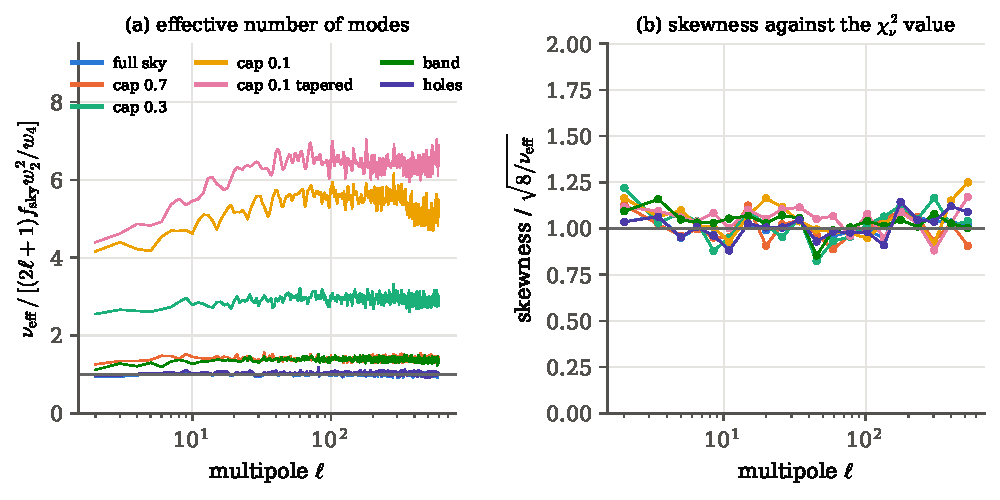
\includegraphics[width=12cm]{figures/ch08/nu_eff.pdf}
\caption{(a) The effective number of modes of a single pseudo-multipole from $\EightBNsim$ skies, divided
by the count $(2\ell+1)\fsky w_2^2/w_4$ of \srcref{Hivon}{(17)}. The smaller the cap, the more each multipole
borrows from its neighbours, and the larger the ratio. (b) The simulated skewness divided by the
$\chi^2_{\nu_{\rm eff}}$ value $\sqrt{8/\nu_{\rm eff}}$: one for every mask, so the moment-matched $\chi^2$ gets the
third moment right too.}
\label{8b:fig:nu-eff}
\end{figure}

What this means for the likelihood is the subject of \cref{ch:09}, but the lesson can be said now,
starting from the observation. \emph{The event:} one sky, and one number from it, the quadrupole
$\widetilde C_2=x$ through the $10\%$ cap. \emph{What could have produced it?} Any true spectrum: every candidate
$C_2$ would have produced skies with a spread of values, and the observed $x$ is one draw. \emph{How
probable is $x$ under each candidate?} The distribution of the estimate, computed for each $C_2$ and
then read at the fixed observed $x$ as a function of $C_2$, answers that; it is the likelihood
(\cref{3b:sec:likelihood,8a:sec:shape}). It measures how readily each candidate spectrum, plus the
fluctuation of one sky, turns into the number we actually saw.

Use the scaled $\chi^2$ just found, with mean $C_2$ and $\nu_{\rm eff}\approx2$ (we measured $\EightBnueffCapTenTwo$). A $\chi^2_2$
has density $\tfrac12e^{-y/2}$, so $x=C_2\,y/2$ has density, and likelihood,
\[
  \Like(C_2)=\frac1{C_2}\,e^{-x/C_2},
\]
against the Gaussian of the same mean and variance,
\[
  \Like_{\rm G}(C_2)=\frac1{\sqrt{2\pi}\,C_2}\,e^{-(x-C_2)^2/2C_2^2}
\]
(a scaled $\chi^2_\nu$ has variance $2C_2^2/\nu=C_2^2$). Compare a candidate twice the observed value with
one equal to it. The exact likelihood gives $\Like(2x)/\Like(x)=\tfrac12e^{-1/2}/e^{-1}=0.82$: a spectrum twice
as large as what we saw is almost as plausible, because a $\chi^2_2$ often falls well below its mean. The
Gaussian gives $\Like_{\rm G}(2x)/\Like_{\rm G}(x)=\tfrac12e^{-1/8}=0.44$, half as much. Where does each peak?
The exact likelihood at $C_2=x$. The Gaussian at $C_2=0.62\,x$ (setting the derivative of
$-\ln C_2-(x-C_2)^2/2C_2^2$ to zero gives $u^2-u-1=0$ for $u=x/C_2$, so $u=1.62$). A Gaussian likelihood of the
same width therefore favours spectra that are too low, because it does not know that most skies fall
below their mean. Hivon et al.\ made the same observation for their Boomerang bins and concluded that at small sky
coverage the likelihood must be modelled as a $\chi^2$ at low $\ell$ \srcref{Hivon}{§4.2}; we repeat their
test in \cref{8b:sec:lit-hivon}.

\subsection{Correlations between multipoles}
\label{8b:sec:corr}

\paragraph{The exact covariance.}
For a Gaussian sky the covariance of the pseudo-spectrum follows from the covariance
\eqref{8b:eq:alm-cov} of the masked coefficients by Wick's theorem. For jointly Gaussian complex
variables with zero mean, $\langle xx^*yy^*\rangle=\langle xx^*\rangle\langle yy^*\rangle+\langle xy\rangle\langle x^*y^*\rangle+\langle xy^*\rangle\langle x^*y\rangle$
(the sum over the ways of pairing the four factors, \cref{3a:sec:cov-noise}). Then
\begin{align}
  \Cov\bigl(\widetilde C_\ell,\widetilde C_{\ell'}\bigr)
  &\eqby{1}\frac1{(2\ell+1)(2\ell'+1)}\sum_{mm'}\Bigl(\langle|\tilde a_{\ell m}|^2|\tilde a_{\ell'm'}|^2\rangle
     -\langle|\tilde a_{\ell m}|^2\rangle\langle|\tilde a_{\ell'm'}|^2\rangle\Bigr) \nonumber\\
  &\eqby{2}\frac1{(2\ell+1)(2\ell'+1)}\sum_{mm'}\Bigl(|\langle\tilde a_{\ell m}\tilde a^*_{\ell'm'}\rangle|^2
     +|\langle\tilde a_{\ell m}\tilde a_{\ell'm'}\rangle|^2\Bigr) \nonumber\\
  &\eqby{3}\frac2{(2\ell+1)(2\ell'+1)}\sum_{mm'}|\langle\tilde a_{\ell m}\tilde a^*_{\ell'm'}\rangle|^2 .
  \label{8b:eq:cov-exact}
\end{align}
\begin{explain}
  \item The definition \eqref{8b:eq:pcl} of $\widetilde C_\ell$ in both factors, and bilinearity of the covariance.
  \item Wick's theorem with $x=\tilde a_{\ell m}$, $y=\tilde a_{\ell'm'}$: the first pairing cancels the product of means,
        and $\langle xy^*\rangle\langle x^*y\rangle=|\langle xy^*\rangle|^2$, $\langle xy\rangle\langle x^*y^*\rangle=|\langle xy\rangle|^2$.
  \item The masked map is real, so $\tilde a_{\ell'm'}=(-1)^{m'}\tilde a^*_{\ell',-m'}$ and
        $|\langle\tilde a_{\ell m}\tilde a_{\ell'm'}\rangle|=|\langle\tilde a_{\ell m}\tilde a^*_{\ell',-m'}\rangle|$; summing over all $m'$, the
        second sum is the first one relabelled.
\end{explain}
This is \cite[eqs~14 and 18]{Efstathiou2004}. On the full sky,
$\langle a_{\ell m}a^*_{\ell'm'}\rangle=\Cell\delta_{\ell\ell'}\delta_{mm'}$, the sum has $2\ell+1$ equal terms, and the covariance is
$2\Cell^2/(2\ell+1)$ on the diagonal and zero elsewhere, as it must be. Through a mask, the covariance
\eqref{8b:eq:alm-cov} connects $(\ell,m)$ to every $(\ell',m')$ the window couples, and the spectrum
inherits those correlations, squared.

\paragraph{An exact calculation for an azimuthal mask.}
For a mask that is the same along every ring of constant latitude, like the band, the exact
covariance can be computed without any $3j$ symbol, because the window cannot change $m$. Write
$Y_{\ell m}=\lambda_{\ell m}(\theta)e^{im\phi}$ with $\lambda_{\ell m}$ real, and do the integral \eqref{8b:eq:K} as the HEALPix pixel
sum: rings $r$ at colatitude $\theta_r$, each with $n_{\phi,r}$ pixels at $\phi_j=\phi_{0,r}+2\pi j/n_{\phi,r}$, all of area
$\Omega_{\rm pix}$ and window value $W_r$. Then
\begin{align}
  K_{\ell m,\ell'm'}
  &\eqby{1}\sum_r\Omega_{\rm pix}W_r\,\lambda_{\ell m}(\theta_r)\lambda_{\ell'm'}(\theta_r)\,e^{i(m'-m)\phi_{0,r}}
     \sum_{j=0}^{n_{\phi,r}-1}e^{2\pi i(m'-m)j/n_{\phi,r}}
   \nonumber\\
  &\eqby{2}\delta_{mm'}\,K^{(m)}_{\ell\ell'},\qquad
  K^{(m)}_{\ell\ell'}\equiv\sum_{\text{rings }r}n_{\phi,r}\,\Omega_{\rm pix}\,W_r\,\lambda_{\ell m}(\theta_r)\lambda_{\ell'm}(\theta_r) .
  \label{8b:eq:K-ring}
\end{align}
\begin{explain}
  \item The pixel sum of $Y^*_{\ell m}WY_{\ell'm'}$; $W$ and $\theta$ are constant along a ring, so only the phase
        $e^{i(m'-m)\phi_j}$ changes from pixel to pixel.
  \item The sum over $j$ is a geometric series in $q=e^{2\pi i(m'-m)/n_{\phi,r}}$, equal to $(1-q^{n_{\phi,r}})/(1-q)=0$ when
        $q\neq1$, because $q^{n_{\phi,r}}=e^{2\pi i(m'-m)}=1$; and equal to $n_{\phi,r}$ when $q=1$, that is $m'=m$ (this needs
        $|m'-m|<n_{\phi,r}$; it can fail only on the few short rings next to the poles, where $\lambda_{\ell m}\propto\sin^{|m|}\theta$
        is negligible for the large $|m|$ concerned).
\end{explain}
The window couples $\ell$ to $\ell'$ but never $m$ to $m'\neq m$. Two covariances follow. The signal enters
through \eqref{8b:eq:alm-cov}, with the beam and pixel window on the true spectrum, and $K$ real and
diagonal in $m$: $\sum_LK^{(m)}_{\ell L}T_L^2C_LK^{(m)}_{\ell'L}$. The noise, white with variance $\sigma^2$ per pixel and
independent between pixels, is masked pixel by pixel, so the step of \eqref{8a:eq:noise-cov-general} picks
up $W_r^2$ in each pixel and the same ring sum applies: $N\sum_rn_{\phi,r}\Omega_{\rm pix}W_r^2\lambda_{\ell m}\lambda_{\ell'm}$, with
$N=\sigma^2\Omega_{\rm pix}$. Together,
$\langle\tilde a_{\ell m}\tilde a^*_{\ell'm}\rangle=\sum_LK^{(m)}_{\ell L}T_L^2C_LK^{(m)}_{\ell'L}+N\sum_rn_{\phi,r}\Omega_{\rm pix}W_r^2\lambda_{\ell m}\lambda_{\ell'm}$.
The functions $\lambda_{\ell m}$ are computed with the standard
three-term recursion in $\ell$ at fixed $m$, which needs no factorials and is stable to $\ell$ of several
thousand (\pyname{lambda_lm} in \pyname{lib_masks.py}). Inserting into \eqref{8b:eq:cov-exact} gives the
exact covariance of the band's pseudo-spectrum at $\ell,\ell'\le\EightBexactL$ in seconds. The ratio of the
simulated variance to the exact one has mean $\EightBexactMCmean$ and scatter $\EightBexactMCrms$ over those
multipoles, which is the $\pm\EightBvarNoise\%$ expected of a variance from $\EightBNsim$ skies: the simulations
and the exact formula agree.

\paragraph{What the correlation matrices look like.}
\Cref{8b:fig:corr-maps} shows the correlation matrix
$\Corr(\widetilde C_\ell,\widetilde C_{\ell'})=\Cov/\sqrt{\Var\,\Var}$ for $2\le\ell,\ell'\le100$ from the simulations, and
\cref{8b:fig:corr-neighbours} the correlation of each multipole with its first and second neighbours.
Three dependences stand out. \emph{On the sky fraction:} the correlation with the next multipole is
$\EightBcorrOneCapSeventy$ for the $70\%$ cap, $\EightBcorrOneCapThirty$ for the $30\%$ cap and $\EightBcorrOneCapTen$ for the $10\%$
cap; with the second neighbour, $\EightBcorrTwoCapSeventy$, $\EightBcorrTwoCapThirty$ and $\EightBcorrTwoCapTen$. The width of the
correlated band in $\ell$ grows as the patch shrinks, as $\pi/\Theta$ for a patch of size $\Theta$. \emph{On the
geometry:} the band has no correlation with its immediate neighbour ($\EightBcorrOneBand$) but
$\EightBcorrTwoBand$ with the next-but-one, the parity selection of \cref{8b:sec:coupling-check} seen in the
covariance; the holes, which remove $3\%$ of the sky in small pieces, correlate nothing
($\EightBcorrOneHoles$). \emph{On apodisation:} the tapered $10\%$ cap is even more correlated than the sharp
one, $\EightBcorrOneCapTenApo$ and $\EightBcorrTwoCapTenApo$, because its effective region is smaller and its kernel
wider. \emph{On $\ell$:} hardly at all; the curves of \cref{8b:fig:corr-neighbours} are flat from $\ell=10$ to
$600$, because the kernel width is set by the patch, not by the multipole. A correlation estimated
from $\EightBNsim$ skies has a noise of $1/\sqrt{\EightBNsim}=\EightBcorrNoise$ (\cref{3a:sec:spurious}), so every value
quoted here is far above noise except those of the holes and the band's first neighbour.

\begin{figure}[htbp]
\centering
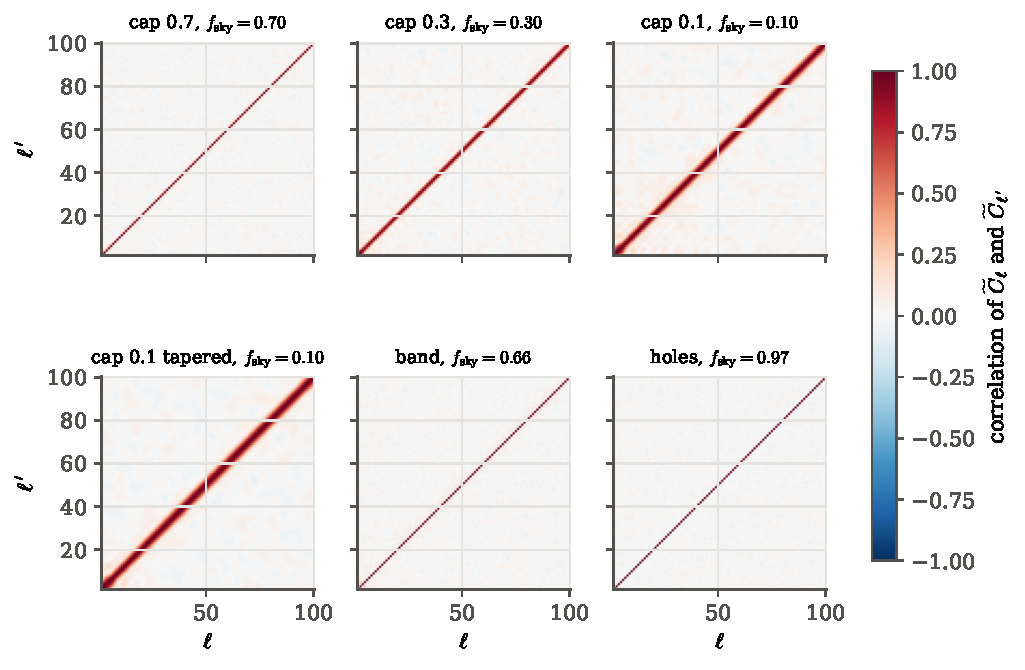
\includegraphics[width=11.5cm]{figures/ch08/corr_maps.pdf}
\caption{Correlation matrices of $\widetilde C_\ell$ for $2\le\ell,\ell'\le100$ from $\EightBNsim$ skies. The diagonal
band widens as the cap shrinks from $70\%$ to $10\%$ and widens further when the $10\%$ cap is tapered.
The band cut and the holes leave the matrix nearly diagonal (the band's correlation with $\ell\pm2$ is
too faint to see at this scale).}
\label{8b:fig:corr-maps}
\end{figure}

\begin{figure}[htbp]
\centering
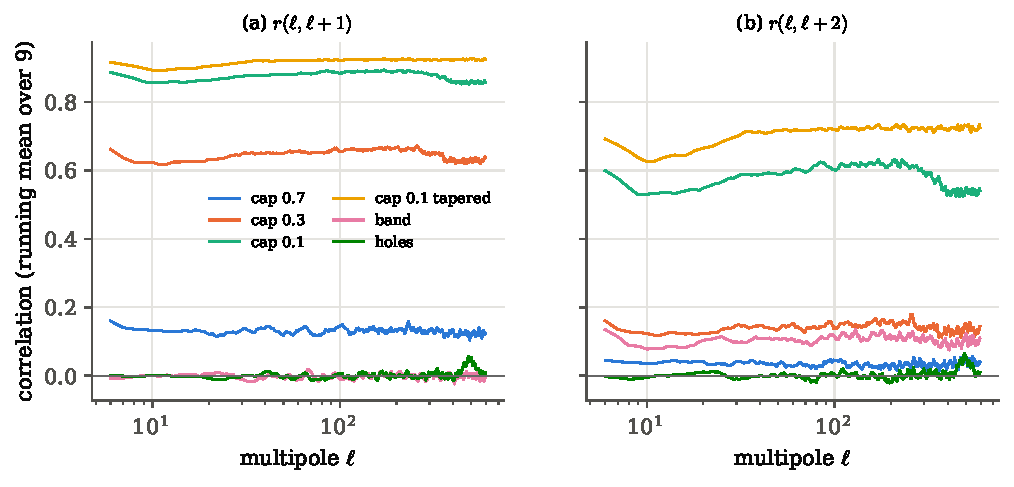
\includegraphics[width=12cm]{figures/ch08/corr_neighbours.pdf}
\caption{Correlation of $\widetilde C_\ell$ with $\widetilde C_{\ell+1}$ (a) and $\widetilde C_{\ell+2}$ (b), smoothed over nine
multipoles. The level is set by the mask and is almost independent of $\ell$. The band correlates only
multipoles of the same parity: zero in (a), nonzero in (b).}
\label{8b:fig:corr-neighbours}
\end{figure}

\subsection{Quick formulas against the simulations}
\label{8b:sec:quick}

\paragraph{Efstathiou's approximation.}
The exact covariance \eqref{8b:eq:cov-exact} needs every element of the $\tilde a$ covariance. There are about
$\ell_{\max}^2$ pairs $(\ell,m)$, so about $\ell_{\max}^4$ elements, and each is a sum \eqref{8b:eq:alm-cov} over another
$\ell_{\max}^2$ pairs $(\ell_1,m_1)$: a cost of order $\ell_{\max}^6$ for a general mask, $2\times10^{17}$ operations at $\ell_{\max}=767$.
\Textcite{Efstathiou2004} found a shortcut for multipoles above the width of the kernel.

\emph{The approximation, and its error.} In the sum \eqref{8b:eq:alm-cov} for $\langle\tilde a_{\ell m}\tilde a^*_{\ell'm'}\rangle$,
the product $K_{\ell m,\ell_1m_1}K^*_{\ell'm',\ell_1m_1}$ is appreciable only for $\ell_1$ within the kernel width of both
$\ell$ and $\ell'$. Write $C_{\ell_1}=\sqrt{\Cell C_{\ell'}}\,(1+\epsilon_{\ell_1})$ there. If the spectrum changes by less than a
fraction $\epsilon$ across the kernel, every $|\epsilon_{\ell_1}|\lesssim\epsilon$, and dropping them changes the sum by a
relative $O(\epsilon)$. For $\ell=\ell'$ the replacement is $C_{\ell_1}\to\Cell$, exact for a spectrum that is
constant across the kernel. Then
\begin{align}
  \langle\tilde a_{\ell m}\tilde a^*_{\ell'm'}\rangle
  &\eqby{1}\sum_{\ell_1m_1}C_{\ell_1}\langle\ell m|\hat W|\ell_1m_1\rangle\langle\ell_1m_1|\hat W|\ell'm'\rangle
   \relby{2}{\approx}\sqrt{\Cell C_{\ell'}}\;\langle\ell m|\hat W^2|\ell'm'\rangle , \nonumber\\
  \Cov\bigl(\widetilde C_\ell,\widetilde C_{\ell'}\bigr)
  &\relby{3}{\approx}\frac{2\Cell C_{\ell'}}{(2\ell+1)(2\ell'+1)}\sum_{mm'}|\langle\ell m|\hat W^2|\ell'm'\rangle|^2
   \eqby{4}2\Cell C_{\ell'}\,\Xi\bigl(\ell,\ell',\mathcal W^{(2)}\bigr),
  \label{8b:eq:efstathiou}
\end{align}
\begin{explain}
  \item \eqref{8b:eq:alm-cov} with $K_{\ell m,\ell_1m_1}=\langle\ell m|\hat W|\ell_1m_1\rangle$ and $K^*_{\ell'm',\ell_1m_1}=\langle\ell_1m_1|\hat W|\ell'm'\rangle$
        ($\hat W$ is real, hence Hermitian).
  \item The approximation, then completeness, $\sum_{\ell_1m_1}|\ell_1m_1\rangle\langle\ell_1m_1|=\Id$: two
        multiplications by $W$ are one multiplication by $W^2$.
  \item Insert into the exact result \eqref{8b:eq:cov-exact}.
  \item The sum over $m,m'$, worked out below.
\end{explain}
For step~4, notice that $\langle\ell m|\hat W^2|\ell'm'\rangle$ is the coupling $K$ of \eqref{8b:eq:K} for a different window,
$W^2$ in place of $W$. Expand $W^2=\sum_{LM}w^{(2)}_{LM}Y_{LM}$, with spectrum $\mathcal W^{(2)}_L$. Then
\begin{align*}
  \sum_{mm'}|\langle\ell m|\hat W^2|\ell'm'\rangle|^2
  &\eqby{1}\frac{(2\ell+1)(2\ell'+1)}{4\pi}\sum_{mm'}\Bigl|\sum_{LM}w^{(2)}_{LM}\sqrt{2L+1}
     \begin{pmatrix}\ell&L&\ell'\\0&0&0\end{pmatrix}\begin{pmatrix}\ell&L&\ell'\\-m&M&m'\end{pmatrix}\Bigr|^2\\
  &\eqby{2}\frac{(2\ell+1)(2\ell'+1)}{4\pi}\sum_{LM}|w^{(2)}_{LM}|^2\begin{pmatrix}\ell&\ell'&L\\0&0&0\end{pmatrix}^2
   \eqby{3}(2\ell+1)(2\ell'+1)\,\Xi\bigl(\ell,\ell',\mathcal W^{(2)}\bigr),
\end{align*}
\begin{explain}
  \item The Gaunt integral \eqref{8b:eq:gaunt}, exactly as in line~2 of \eqref{8b:eq:M}, with $w^{(2)}$ for $w$; the
        sign $(-1)^m$ has modulus one and has been dropped.
  \item The collapse \eqref{8b:eq:3j-collapse} with $c_{LM}=w^{(2)}_{LM}\sqrt{2L+1}\,(\ell\;L\;\ell';0\;0\;0)$, and the squared
        symbol is symmetric in its columns.
  \item $\sum_M|w^{(2)}_{LM}|^2=(2L+1)\mathcal W^{(2)}_L$, and the definition
        $\Xi(\ell,\ell',\mathcal W)\equiv\sum_L\frac{2L+1}{4\pi}\mathcal W_L(\ell\;\ell'\;L;0\;0\;0)^2$.
\end{explain}
Each element of the approximate covariance is now one sum over $L$, about $\ell_{\max}$ terms, for each of the
$\ell_{\max}^2$ pairs $(\ell,\ell')$: a cost of order $\ell_{\max}^3$, $4.5\times10^8$ operations at $\ell_{\max}=767$, against $2\times10^{17}$.
This is \cite[eqs~15a--15b]{Efstathiou2004}. For a binary mask $W^2=W$, and the covariance is
$2\Cell C_{\ell'}G_{\ell\ell'}$ with the symmetric coupling matrix $G=M/(2\ell'+1)$ \cite[eq.~16]{Efstathiou2004};
for the deconvolved estimate it is $M^{-1}V(M^{-1})\T$ \cite[eq.~17]{Efstathiou2004}, and for MASTER
bandpowers the same with $K^{-1}P$. With beam and noise, $\Cell$ is the spectrum of the field that was
masked, $T_\ell^2\Cell+N$. A common refinement replaces it by the coupled spectrum
$\sum_{\ell'}M_{\ell\ell'}(T^2_{\ell'}C_{\ell'}+N)/\fsky w_2$, which already contains the power that leaked in from
elsewhere.

\begin{keyidea}[Covariance of the cut-sky spectrum]
For a Gaussian sky,
$\Cov(\widetilde C_\ell,\widetilde C_{\ell'})=\frac{2}{(2\ell+1)(2\ell'+1)}\sum_{mm'}|\langle\tilde a_{\ell m}\tilde a^*_{\ell'm'}\rangle|^2$ exactly.
Above the width of the coupling kernel it is approximately $2\Cell C_{\ell'}\,\Xi(\ell,\ell',\mathcal W^{(2)})$: the
full-sky cosmic variance spread over neighbouring multipoles by the spectrum of the \emph{squared}
window. Below it, only the exact form or simulations will do.
\end{keyidea}

\paragraph{How good is it?}
\Cref{8b:fig:efstathiou}a divides the approximation's variance of $\widetilde C_\ell$ by the simulated one.
At high $\ell$ ($100$--$600$) the plain approximation gives $\EightBefsHighCapSeventy$ ($70\%$ cap), $\EightBefsHighCapThirty$
($30\%$), $\EightBefsHighCapTen$ ($10\%$), $\EightBefsHighBand$ (band) and $\EightBefsHighHoles$ (holes); with the coupled
spectrum the same ratios become $\EightBimpHighCapSeventy$, $\EightBimpHighCapThirty$, $\EightBimpHighCapTen$, $\EightBimpHighBand$ and
$\EightBimpHighHoles$. The refinement matters exactly where leakage matters: sharp, small or holey masks at
high $\ell$, where the power that leaked in from the acoustic peaks carries its own variance. At low
$\ell$ the approximation fails, as it was designed to. At $\ell=2$ it is off by factors of $\EightBefsTwoCapThirty$
and $\EightBefsTwoCapTen$ for the $30\%$ and $10\%$ caps, at $\ell=10$ by $\EightBefsTenCapThirty$ and $\EightBefsTenCapTen$.
Against the exact band covariance (\cref{8b:fig:efstathiou}b) the approximation is $\EightBexactApproxTwo$ times
the truth at $\ell=2$, $\EightBexactApproxFour$ at $\ell=4$, $\EightBexactApproxTwenty$ at $\ell=20$ and $\EightBexactApproxForty$ at
$\ell=40$. Efstathiou found the same pattern for a $\pm10^\circ$ cut, accurate at $\ell\gtrsim20$ and wrong by up to
$25\%$ at $\ell=2$ \cite[§2.2]{Efstathiou2004}; our $\pm20^\circ$ cut removes twice as much and the low-$\ell$
error is correspondingly larger.

\begin{figure}[htbp]
\centering
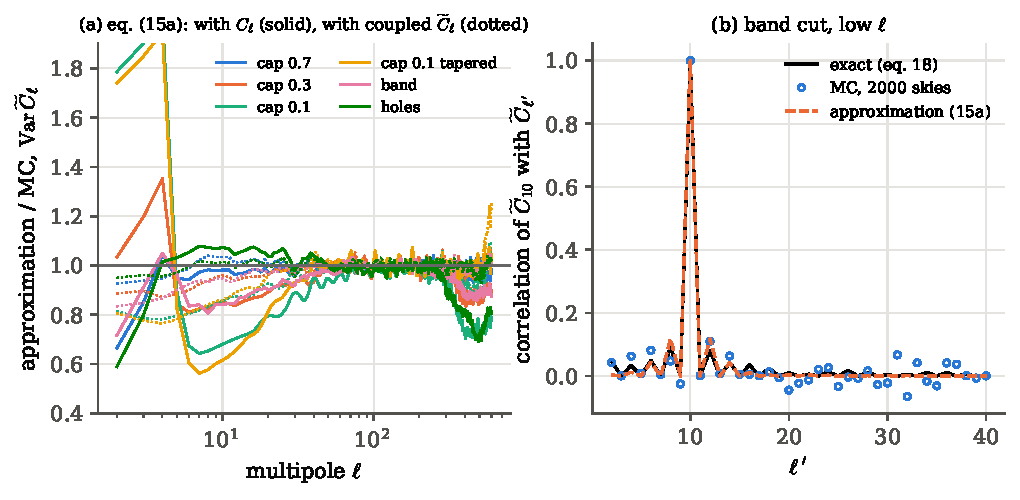
\includegraphics[width=12.5cm]{figures/ch08/efstathiou.pdf}
\caption{(a) Efstathiou's approximation \eqref{8b:eq:efstathiou} for the variance of $\widetilde C_\ell$, divided by
the simulated variance, for six masks: with the masked spectrum (solid) and with the coupled spectrum
(dotted). Above $\ell\approx30$ it is good to a few per cent with the refinement; at low $\ell$ it fails by large
factors. (b) The band cut: correlation of $\widetilde C_{10}$ with $\widetilde C_{\ell'}$, exact from \eqref{8b:eq:K-ring} (black),
from $\EightBNsim$ skies (blue circles) and from the approximation (orange dashed). Only multipoles of the
same parity as $\ell=10$ are correlated, and the three agree on the pattern.}
\label{8b:fig:efstathiou}
\end{figure}

\paragraph{Knox's formula, for the MASTER bins.}
The simplest error bar of all is the mode-counting rule of \cref{8a:sec:knox},
$\Var\widehat D_b=2(D_b+N_b)^2/[(2\ell_b+1)\Delta\ell\,\fsky]$, with $N_b$ the binned noise on the sky. \Cref{8b:fig:knox-mc}
divides the simulated variance of the MASTER bandpowers (bins of $20$) by it. On the full sky the ratio is
$\EightBknoxHighFull$ at high $\ell$ and $\EightBknoxFirstFull$ in the first bin, the full-sky verification of
\cref{8a:sec:res-var} in another guise. Through the masks it is larger than one almost everywhere and
grows as the patch shrinks: at high $\ell$, $\EightBknoxHighCapSeventy$ for the $70\%$ cap, $\EightBknoxHighCapThirty$ for $30\%$,
$\EightBknoxHighCapTen$ for $10\%$ and $\EightBknoxHighBand$ for the band. The holes are fine at low $\ell$ ($\EightBknoxSecondHoles$)
and worst at the highest multipoles ($\EightBknoxHighHoles$), where the leaked power of the peaks adds variance
that mode counting knows nothing about. For the tapered cap the version with Hivon's $w_2^2/w_4$ gives
$\EightBknoxHighCapTenApo$, while $\fsky$ alone gives $\EightBknoxOnlyHighCapTenApo$, the pitfall of \cref{8b:sec:pseudo} in
numbers. The Monte Carlo error of each ratio is $\EightBvarNoise\%$.

\begin{figure}[htbp]
\centering
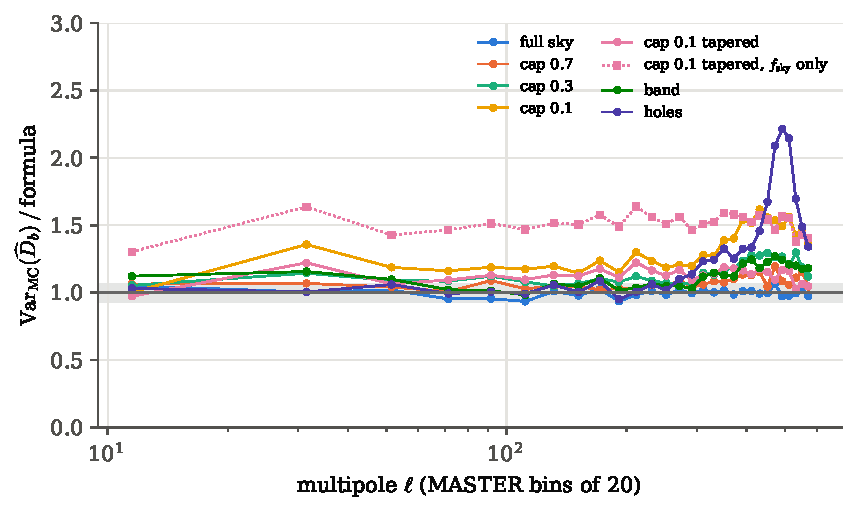
\includegraphics[width=10.5cm]{figures/ch08/knox_mc.pdf}
\caption{Simulated variance of the MASTER bandpowers divided by the mode-counting formula, bins of
$20$ multipoles. The full sky sits on one; the smaller the patch, the larger the excess. For the
tapered cap the formula with $\fsky w_2^2/w_4$ (solid pink) does much better than with $\fsky$ alone
(dotted pink). The holes rise at the highest multipoles, where leakage dominates.}
\label{8b:fig:knox-mc}
\end{figure}

Why is the excess there at all, in a bin of $20$ multipoles, many times wider than the kernel? The
counting formula is the variance of an \emph{optimal} estimate from the modes the patch contains. MASTER
is not optimal: it weights every pixel of the window equally whatever the signal-to-noise, and the
deconvolution $K^{-1}$ undoes the smoothing of the coupling. Undoing a smoothing amplifies the
scatter, and a two-bin toy shows by how much. The MASTER bandpowers are $\widehat{\bm D}=K^{-1}\bm y$ with
$\bm y=P(\widetilde{\bm C}-\langle\widetilde{\bm N}\rangle)$, so their covariance is $K^{-1}\Cov(\bm y)(K^{-1})\T$. Take two bins with
unit diagonal and coupling $c$ between them, and give the two binned pseudo-spectra equal variance
$\sigma^2$ and no correlation:
\begin{align*}
  K=\begin{pmatrix}1&c\\c&1\end{pmatrix},\quad
  K^{-1}&\eqby{1}\frac1{1-c^2}\begin{pmatrix}1&-c\\-c&1\end{pmatrix},\quad
  \Var\widehat D_1\eqby{2}\sigma^2\,\frac{1+c^2}{(1-c^2)^2} .
\end{align*}
\begin{explain}
  \item The inverse of a $2\times2$ matrix: swap the diagonal, negate the off-diagonal, divide by the
        determinant $1-c^2$.
  \item $\widehat D_1=(y_1-cy_2)/(1-c^2)$, and the variances of independent terms add: $\sigma^2(1+c^2)/(1-c^2)^2$.
\end{explain}
The factor exceeds one for every $c\neq0$ and grows with $c$: $1.13$ for $c=0.2$, $1.32$ for $c=0.3$. The inverse
has a negative off-diagonal entry, the ``wing'' that subtracts the neighbour's leaked power, and that
subtraction brings in the neighbour's scatter too (the long negative wings of $K^{-1}$ in
\cref{8b:fig:boom-kernel} are the same thing for a real patch). A wider kernel means larger couplings
between bins, so the amplification grows as the patch shrinks. A $40\%$ excess in the variance is an
excess of $\sqrt{1.40}=1.18$, or $18\%$, in the error bar, the price of an estimator that is fast and
unbiased. Efstathiou showed that at high $\ell$ the
pseudo-$\Cell$ estimator with suitable weights is nonetheless nearly as good as the optimal quadratic one
\cite[§§3--5]{Efstathiou2004}, and that at low $\ell$ the optimal one should be used instead, the hybrid
strategy of real analyses (\cref{8b:sec:research}).

\begin{pitfall}[Quick covariances at low $\ell$]
Both the mode-counting formula and Efstathiou's approximation assume that the spectrum is constant
across the coupling kernel. At low $\ell$, and for any patch smaller than a hemisphere, they are wrong
by tens of per cent to factors of several, and the distribution is not Gaussian anyway. Use the exact
expression \eqref{8b:eq:cov-exact} (cheap at low resolution), or simulations, for the multipoles
below a few times $\pi/\Theta$.
\end{pitfall}

The laptop version of these tests uses $\EightBNsim$ Gaussian skies at $N_{\rm side}=\EightBnside$, which measure each
variance to $\EightBvarNoise\%$ and each correlation to $\pm\EightBcorrNoise$; a research covariance is built from a few
hundred end-to-end simulations at full resolution together with an analytic model of the
Efstathiou type that includes the noise and the beam for every pair of maps, and the simulations
serve to validate and correct the model rather than to replace it \cite{Planck2018V}. What the
reduction costs is resolution ($\ell\le767$ instead of $2500$) and realism (no foreground residuals, no
correlated noise), not the logic of the test.
\section{How many simulations?}
\label{8b:sec:nsims}

Everything in \cref{8b:sec:distribution} came from $\EightBNsim$ simulated skies, and the next step of a
real analysis puts the simulated covariance into a likelihood: the probability of the bandpowers
$\widehat{\bm D}$ we actually observed, read as a function of the parameters $\params$. For each $\params$ the model
predicts $\bm D(\params)$, and the question is how probable the fluctuation $\widehat{\bm D}-\bm D(\params)$ is that would turn
that prediction into our data (\cref{3b:sec:likelihood}). For Gaussian bandpowers that probability is
proportional to $\exp[-\frac12(\widehat{\bm D}-\bm D)\T\Cmat^{-1}(\widehat{\bm D}-\bm D)]$, so
$-2\ln\Like=(\widehat{\bm D}-\bm D)\T\Cmat^{-1}(\widehat{\bm D}-\bm D)$ plus a constant, and it needs the inverse of
the covariance, the \newterm{precision matrix}. Take the MASTER bandpowers of the $30\%$ cap of
\cref{8b:sec:binning}: $p=\EightBpcov$ bins of $20$ multipoles below $\ell=600$, with neighbouring bins
correlated through the mask. With $\EightBNall$ simulations the covariance is good to a few per cent.
A full-resolution end-to-end simulation of a real experiment costs hours, not a second, and a few
hundred of them is a typical budget. The question is how few we can afford, and what goes wrong when
there are too few. Two different things go wrong, and they need to be kept apart: the elements of
the estimated covariance are noisy, and the inverse of a noisy matrix is biased.

\subsection{Noise in the elements}
\label{8b:sec:cov-element-noise}

The sample covariance from $N$ independent Gaussian draws has, element by element, the variance
$(\Sigma_{aa}\Sigma_{bb}+\Sigma_{ab}^2)/(N-1)$ of \eqref{3a:eq:var-cov-element}. On the diagonal that is a relative error
$\sqrt{2/(N-1)}$, and for a correlation coefficient near zero an absolute error of about
$1/\sqrt N$. To see this on the CMB, script \pyname{28_nsims.py} draws subsets of $N$ skies from the
$\EightBNall$ and compares each subset's covariance with the one from all of them. Because the reference is
itself built from a finite set, the subset fluctuates around it with a variance smaller by the
finite-population factor $1-N/N_{\rm all}$: a subset that is the whole set does not fluctuate at all.
At $N=100$ the measured rms error is $\EightBdiagErrHundred$ on the diagonal, and
$\sqrt{2/99}\times\sqrt{1-100/2000}=0.139$; for the correlations it is $\EightBoffErrHundred$, and
$\sqrt{1/100}\times\sqrt{0.95}=0.098$ (\cref{8b:fig:cov-noise}).

\begin{figure}[htbp]
\centering
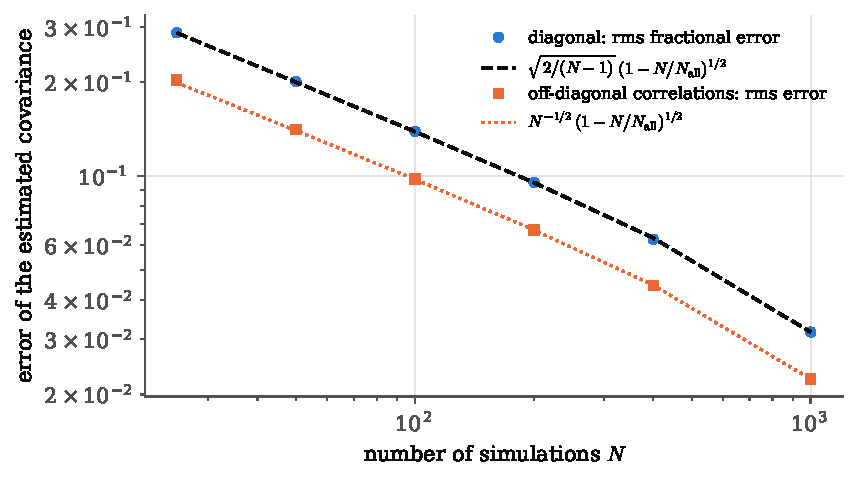
\includegraphics[width=10cm]{figures/ch08/cov_noise.pdf}
\caption{Noise in a covariance estimated from $N$ of the $\EightBNall$ simulated skies, for the $\EightBpcov$ MASTER
bins of the $30\%$ cap. Blue: rms relative error of the diagonal elements; orange: rms error of the
off-diagonal correlation coefficients. The lines are $\sqrt{2/(N-1)}$ and $1/\sqrt N$, each with the
finite-population factor $(1-N/N_{\rm all})^{1/2}$.}
\label{8b:fig:cov-noise}
\end{figure}

\paragraph{Example: can we see the correlations at all?}
The $70\%$ cap correlates neighbouring multipoles at $r=\EightBcorrOneCapSeventy$ (\cref{8b:sec:corr}). To detect that
at three standard deviations from a covariance estimated from $N$ skies we need
$3/\sqrt N<\EightBcorrOneCapSeventy$, so $N>(3/\EightBcorrOneCapSeventy)^2\approx530$. With $100$ skies such a correlation is
indistinguishable from the spurious ones that every pair of bins shows at the level of $\pm0.1$. The
correlations that matter for a likelihood are often exactly this small, and many of them add up.

\subsection{Why the inverse is biased}
\label{8b:sec:hartlap}

Inverting a matrix is a nonlinear operation, and the average of a nonlinear function of a noisy
quantity is not the function of its average. Inversion is not just nonlinear but convex: a
fluctuation of the variance towards zero raises its inverse by more than a fluctuation of the same
size away from zero lowers it. Jensen's inequality, $\E[1/X]\ge1/\E[X]$ for a positive random $X$, makes
the inverse of an unbiased covariance biased high. How much is a calculation that starts with one bin.

\paragraph{One bin.}
With $p=1$ and $N=n$ draws, the sample variance (mean subtracted) is $s^2=\sigma^2\chi^2_k/k$ with
$k=n-1$ degrees of freedom (\cref{ch:03}). Then
\begin{align}
  \E\Bigl[\frac1{s^2}\Bigr]
  &\eqby{1}\frac k{\sigma^2}\E\Bigl[\frac1{\chi^2_k}\Bigr]
   \eqby{2}\frac k{\sigma^2}\int_0^\infty\frac1x\,\frac{x^{k/2-1}e^{-x/2}}{2^{k/2}\Gamma(k/2)}\,\dd x
   \eqby{3}\frac k{\sigma^2}\,\frac{2^{k/2-1}\Gamma(k/2-1)}{2^{k/2}\Gamma(k/2)}
   \eqby{4}\frac{k}{k-2}\,\frac1{\sigma^2} .
  \label{8b:eq:inv-chi2}
\end{align}
\begin{explain}
  \item $1/s^2=(k/\sigma^2)/\chi^2_k$, and constants come out of the expectation.
  \item The $\chi^2_k$ density.
  \item The integrand is $x^{(k/2-1)-1}e^{-x/2}$, a gamma integral equal to $\Gamma(k/2-1)\,2^{k/2-1}$; it
        converges for $k>2$.
  \item $\Gamma(k/2)=(k/2-1)\Gamma(k/2-1)$, so the ratio is $\frac12/(k/2-1)=1/(k-2)$.
\end{explain}
With $k=n-1$ the bias factor is $(n-1)/(n-3)$: $11\%$ for $20$ simulations, harmless for a thousand.

\paragraph{Many bins.}
For $p$ bins the same mechanism acts in each direction, and the number of directions makes it worse.
Collect the $k=n-1$ mean-subtracted draws (after the rotation of \cref{3a:sec:cov-noise}, $k$ independent
vectors $\bm z_j\sim\Normal(\bm0,\Sigma)$) into $A=\sum_{j=1}^k\bm z_j\bm z_j\T=k\widehat\Cmat$, a Wishart matrix. Look at one
diagonal element of its inverse, say the first. Block inversion of a symmetric matrix gives
\begin{align}
  \frac1{(A^{-1})_{11}}
  &\eqby{1}A_{11}-A_{1r}A_{rr}^{-1}A_{r1}
   \eqby{2}\min_{\bm\beta}\sum_{j=1}^k\bigl(z_{1j}-\bm\beta\T\bm z_{r,j}\bigr)^2
   \;\sim\;\sigma^2_{1\given r}\,\chi^2_{k-(p-1)},
  \label{8b:eq:schur}
\end{align}
\begin{explain}
  \item The Schur complement: for a matrix split into the first index and the rest ($r$), the inverse's
        $(1,1)$ element is one over $A_{11}-A_{1r}A_{rr}^{-1}A_{r1}$.
  \item That expression is the residual sum of squares of the least-squares fit of the first component on
        the other $p-1$ components across the $k$ draws ($\hat{\bm\beta}=A_{rr}^{-1}A_{r1}$). For Gaussian draws the residual
        of $z_1$ given the others is Gaussian with the conditional variance $\sigma^2_{1\given r}$, and a fit with $p-1$
        coefficients leaves a $\chi^2$ with $k-(p-1)$ degrees of freedom (\cref{ch:03}); this holds for any values of
        the regressors, hence also on average over them.
\end{explain}
The conditional variance is again a Schur complement, of the true covariance:
$\sigma^2_{1\given r}=\Sigma_{11}-\Sigma_{1r}\Sigma_{rr}^{-1}\Sigma_{r1}=1/(\Sigma^{-1})_{11}$. So $(A^{-1})_{11}$ is $(\Sigma^{-1})_{11}$ divided by a
$\chi^2_{n-p}$ variable, and \eqref{8b:eq:inv-chi2} with $k\to n-p$ gives its mean:
\begin{align}
  \E\bigl[(\widehat\Cmat^{-1})_{11}\bigr]
  &\eqby{1}k\,\E\bigl[(A^{-1})_{11}\bigr]
   \eqby{2}\frac{n-1}{n-p-2}\,(\Sigma^{-1})_{11}.
  \label{8b:eq:hartlap-derived}
\end{align}
\begin{explain}
  \item $\widehat\Cmat=A/k$, so $\widehat\Cmat^{-1}=kA^{-1}$, with $k=n-1$.
  \item $\E[1/\chi^2_{n-p}]=1/(n-p-2)$ from \eqref{8b:eq:inv-chi2}.
\end{explain}
Nothing was special about the first index: in a rotated basis any unit vector $\bm u$ can be the first
axis, so $\bm u\T\E[\widehat\Cmat^{-1}]\bm u=\frac{n-1}{n-p-2}\bm u\T\Sigma^{-1}\bm u$ for every $\bm u$, and two symmetric matrices with
equal quadratic forms are equal. The whole precision matrix is biased by the same factor
\cite[eq.~16]{Hartlap2007}.

\begin{keyidea}[The Hartlap factor, and why it is there]
For a covariance estimated from $n$ Gaussian simulations of $p$ bins ($p<n-2$),
\[
  \E\bigl[\widehat\Cmat^{-1}\bigr]=\frac{n-1}{n-p-2}\,\Cmat^{-1},\qquad
  \widehat{\Cmat^{-1}}=\frac{n-p-2}{n-1}\,\widehat\Cmat^{-1}\ \text{is unbiased}
\]
\cite[eq.~17]{Hartlap2007}. Each direction of the inverse is one over a residual variance, and fitting
the other $p-1$ directions costs $p-1$ degrees of freedom: the noisy matrix ``explains away'' part of
every fluctuation, its small eigenvalues come out too small, and the inverse too large.
\end{keyidea}

This is the factor quoted in \eqref{3a:eq:hartlap}; there it was stated, here it has been derived.
Two more facts complete the picture \cite[§§2.2, 4]{Hartlap2007}. For $p>n-1$ the sample covariance is
singular, because $n-1$ mean-subtracted vectors span at most $n-1$ dimensions, and no factor can
rescue it. And the sample mean and the sample covariance of Gaussian draws are independent, so a
$\chi^2$ built from both is unbiased once the Hartlap factor is applied; a marginalised likelihood and a
Fisher matrix are still biased by smaller, model-dependent amounts (about $8\%$ in the likelihood, and
up to $30\%$ in $\sqrt{\det\Fish^{-1}}$ as $p/n\to1$, in their examples).

\paragraph{Example: what forty bins and sixty simulations do.}
For $n=60$ and $p=40$ the factor is $(60-40-2)/(60-1)=0.305$: without the correction every $\chi^2$ is three
times too large, and every error bar $\sqrt{3.3}=1.8$ times too small.

\subsection{Testing the Hartlap factor}
\label{8b:sec:hartlap-test}

\paragraph{Hartlap et al.'s experiment, repeated.}
Their test \cite[§3.2, Fig.~1]{Hartlap2007} draws $n=60$ Gaussian vectors of $p_1=240$ bins, from three
population covariances (constant diagonal, linearly falling diagonal, and a non-diagonal
$\sigma^2/(1+\epsilon|i-j|)$ with $\epsilon=0.05$, their eqs~18--20), rebins them to $p=240/j$ bins by joining $j$
neighbours, and compares the trace of the true precision matrix with the trace of the estimated one. We
repeat it with $\EightBhartlapRep$ repetitions instead of their $10^4$ (\cref{8b:fig:hartlap}a). At $p=\EightBhartlapPforty$ the
raw ratio is $\EightBhartlapRawForty$ against the predicted $(n-p-2)/(n-1)=\EightBhartlapPredForty$, and after the correction every
model and every $p$ lies within $\EightBhartlapCorWorst$ of one.

\paragraph{The same on the CMB.}
The sky is not a Gaussian vector of bandpowers: the bandpowers are quadratic in a Gaussian field and,
at low $\ell$, skewed. To see whether the factor still holds we take subsets of $n$ skies from the
$\EightBNall$, invert the covariance of their $p=\EightBpcov$ MASTER bins and compare with the precision matrix from
all of them (\cref{8b:fig:hartlap}b). At $n=60$ the trace ratio is $\EightBcmbRatioSixty$, and the Hartlap factor is
$\EightBcmbHartSixty$. The reference itself carries the factor $(\EightBNall-\EightBpcov-2)/(\EightBNall-1)=\EightBhartlapAll$, a $1.5\%$
correction even with two thousand simulations.

\begin{figure}[htbp]
\centering
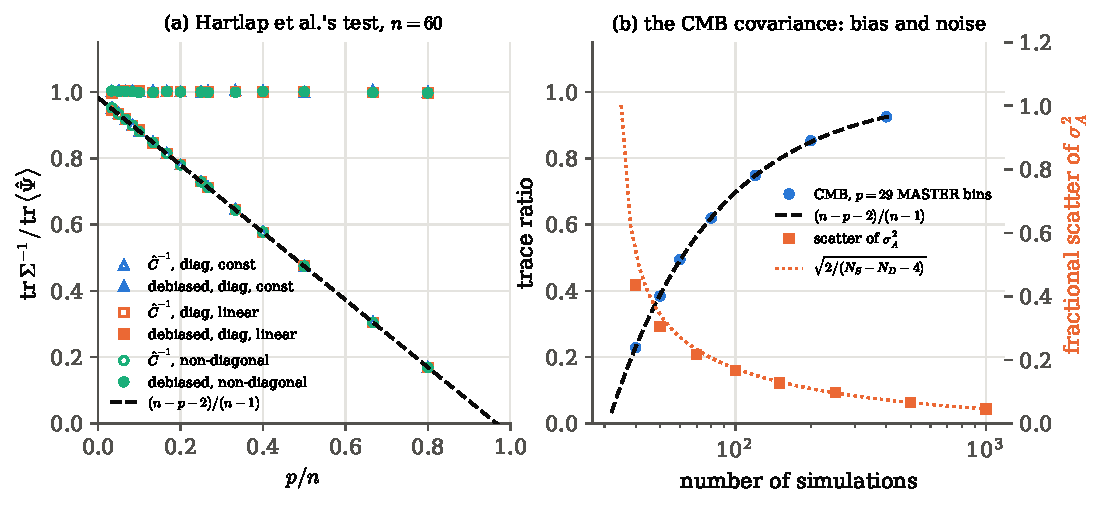
\includegraphics[width=12.5cm]{figures/ch08/hartlap.pdf}
\caption{(a) Hartlap et al.'s test: the trace of the true precision matrix divided by that of the
estimated one, for $n=60$ and $p$ up to $60$, three covariance models (shapes), raw (open) and corrected
(filled). The raw points follow $(n-p-2)/(n-1)$ (dashed) down to zero; the corrected ones sit at one.
(b) The CMB: the same ratio for the MASTER bins of the $30\%$ cap from subsets of $n$ skies (blue, left
axis), on the Hartlap curve; and the scatter of the fitted amplitude's variance (orange, right axis)
against Taylor et al.'s $\sqrt{2/(N_S-N_D-4)}$ (dotted).}
\label{8b:fig:hartlap}
\end{figure}

\subsection{From an unbiased precision matrix to a trustworthy error bar}
\label{8b:sec:taylor}

An unbiased precision matrix is still a noisy one, and its noise reaches the parameters.
\Textcite{Taylor2013} worked out how. Their result for the fractional scatter of a parameter's
variance, estimated with a Hartlap-corrected precision matrix from $N_S$ simulations of $N_D$ data
points, is $\varepsilon=\sqrt{2/(N_S-N_D-4)}$ \cite[eq.~55]{Taylor2013}, and it leads to a planning rule:
\begin{equation}
  N_S>\frac2{\varepsilon^2}+N_D+4
  \qquad\text{\cite[eq.~58]{Taylor2013}}.
  \label{8b:eq:taylor}
\end{equation}
The first term is the familiar $1/\sqrt{N}$ of any average; the second says that each data point costs
one more simulation, the same degrees of freedom that appeared in the Hartlap factor. For a parameter
error good to $5\%$ the variance must be good to $10\%$, $\varepsilon=0.1$, and \eqref{8b:eq:taylor} asks for
$200+N_D+4$ simulations: $\EightBtaylorFivePct$ for our $\EightBpcov$ bins.

\paragraph{The simplest case, exactly.}
For one parameter the calculation of \eqref{8b:eq:schur} gives the whole distribution. Fit an amplitude $A$
of the fiducial spectrum, $\bm D=A\bm t$ with $\bm t$ the fiducial bandpowers.

\emph{Its error bar.} With a precision matrix $\Psi$ the likelihood is quadratic in $A$:
$-2\ln\Like(A)=A^2\,\bm t\T\Psi\bm t-2A\,\bm t\T\Psi\widehat{\bm D}+\text{const}$. A Gaussian in $A$ of width $\sigma_A$ has
$-2\ln\Like=(A-\hat A)^2/\sigma_A^2+\text{const}$, and matching the coefficients of $A^2$ gives
$\sigma_A^2=1/(\bm t\T\Psi\bm t)$, one over the Fisher information (\cref{ch:10}; the full chain is in
\cref{8b:sec:research-run}). With the true covariance, $\sigma_A^2=1/(\bm t\T\Cmat^{-1}\bm t)$.

\emph{Its distribution.} Whiten the data: $\Cmat^{-1/2}$ turns the simulated vectors into draws with identity
covariance, and their sample covariance into $\widehat S=\Cmat^{-1/2}\widehat\Cmat\,\Cmat^{-1/2}$. With $\bm s=\Cmat^{-1/2}\bm t$ and the
unit vector $\bm u=\bm s/|\bm s|$,
\begin{align*}
  \bm t\T\widehat\Cmat^{-1}\bm t
  &\eqby{1}\bm s\T\widehat S^{-1}\bm s
   \eqby{2}|\bm s|^2\,\bigl(\widehat S'^{-1}\bigr)_{11}
   \eqby{3}\frac1{\sigma_A^2}\,\frac{n-1}{\chi^2_{n-p}} .
\end{align*}
\begin{explain}
  \item $\widehat\Cmat^{-1}=\Cmat^{-1/2}\widehat S^{-1}\Cmat^{-1/2}$.
  \item Rotate the basis so that $\bm u$ is the first axis; whitened Gaussian draws stay independent standard
        Gaussians under a rotation, and $\widehat S'$ is their sample covariance in the new basis.
  \item $|\bm s|^2=\bm t\T\Cmat^{-1}\bm t=1/\sigma_A^2$. For $\widehat S'=A/(n-1)$, \eqref{8b:eq:schur} with $\Sigma=\Id$ (so
        $\sigma^2_{1\given r}=1$) says $1/(A^{-1})_{11}\sim\chi^2_{n-p}$, hence $(\widehat S'^{-1})_{11}=(n-1)/\chi^2_{n-p}$.
\end{explain}
Multiplying the inverse by the Hartlap factor, $\Psi=\frac{n-p-2}{n-1}\widehat\Cmat^{-1}$, gives
\begin{equation}
  \widehat{\sigma^2_A}=\frac{n-1}{n-p-2}\,\frac1{\bm t\T\widehat\Cmat^{-1}\bm t}
  =\sigma_A^2\,\frac{\chi^2_{n-p}}{n-p-2},
  \qquad
  \frac{\E\,\widehat{\sigma^2_A}}{\sigma^2_A}=\frac{n-p}{n-p-2},\qquad
  \frac{\sigma\bigl(\widehat{\sigma^2_A}\bigr)}{\E\,\widehat{\sigma^2_A}}=\sqrt{\frac2{n-p}} .
  \label{8b:eq:sigA}
\end{equation}
Even with the unbiased precision matrix, the parameter's variance is biased \emph{high}, for the same
convexity reason as before: $\sigma_A^2$ is one over a linear function of $\Psi$. The test of
\pyname{28_nsims.py} draws $n$ Gaussian bandpower vectors from the CMB covariance ($\sigma_A=\EightBsigAtrue$ with the
true precision matrix), $\EightBNall$ times for each $n$. At $n=40$ the mean of $\widehat{\sigma^2_A}$ is high by
$\EightBtaylorBiasForty\%$, and \eqref{8b:eq:sigA} gives $(40-29)/(40-31)=1.22$; its fractional scatter is $\EightBtaylorScatForty$,
against $\sqrt{2/11}=0.43$ from \eqref{8b:eq:sigA} and $\EightBtaylorPredForty$ from Taylor et al.'s general formula. At
$n=100$ the scatter is $\EightBtaylorHundred$, against $\sqrt{2/71}=0.168$ and $\EightBtaylorPredHundred$. For a single parameter
\eqref{8b:eq:sigA} is exact.

\emph{What the ``$-4$'' covers.} The same calculation shows where Taylor et al.'s formula sits. Their
expression is the relative scatter of the \emph{information} $\bm t\T\Psi\bm t=1/\widehat{\sigma^2_A}$, which is proportional to
$1/\chi^2_k$ with $k=n-p$. From the gamma integral of \eqref{8b:eq:inv-chi2}, $\E[1/\chi^2_k]=1/(k-2)$ and
$\E[1/(\chi^2_k)^2]=1/[(k-2)(k-4)]$, so
\[
  \Var\frac1{\chi^2_k}=\frac1{(k-2)(k-4)}-\frac1{(k-2)^2}=\frac2{(k-2)^2(k-4)},\qquad
  \frac{\sigma(1/\chi^2_k)}{\E(1/\chi^2_k)}=\sqrt{\frac2{k-4}}=\sqrt{\frac2{N_S-N_D-4}} .
\]
The variance itself is proportional to $\chi^2_k$, whose relative scatter is $\sqrt{2/k}$. The two agree when
$k$ is large, because a small relative error of a quantity is also the relative error of its inverse;
at $k=11$ the inverse $\chi^2$, with its longer tail, scatters more. The ``$-4$'' is that tail, and a planning
rule built on it errs on the safe side.

\begin{pitfall}[Too few simulations cannot be repaired]
When $p\ge n-1$ the sample covariance is singular. A pseudo-inverse obtained by discarding small singular
values produces a finite matrix, but its bias depends on the covariance model and is not removed by any
factor \cite[§3.2]{Hartlap2007}. Plan the simulations so that $n-p$ is comfortably larger than
$2/\varepsilon^2$, compress the data into fewer bins, or model the covariance analytically and use simulations only
to test the model.
\end{pitfall}

\paragraph{What our numbers are worth.}
Our covariance uses $\EightBNall$ skies for $\EightBpcov$ bins. The Hartlap factor is $\EightBhartlapAll$, and by
\eqref{8b:eq:sigA} the variance of a single parameter is uncertain by $\sqrt{2/1971}=3.2\%$, its error bar by
$1.6\%$. A research analysis has larger data vectors and dearer simulations. Planck's $300$ end-to-end
simulations \cite{Planck2018V} would give, for a vector of a few hundred bandpowers, an $n-p$ of order
one hundred and a $14\%$ uncertainty on each parameter variance. That is why the high-$\ell$ likelihoods of
Planck and of the ground-based experiments use analytic covariances of the Efstathiou type, with the
simulations used to test and correct them: the cost of a reduction in simulations is paid in the
precision of the error bars, and the cure is to need fewer simulations, not to pretend that a small
number is enough.
\section{Reproducing the cut-sky literature}
\label{8b:sec:literature}

The full-sky content of Knox (1995) and Hivon et al.\ (2002) was reproduced in
\cref{8a:sec:literature}. The papers behind this part of the chapter make claims about masked skies,
and each of them can be put to the same test: rebuild the experiment with our own code, at laptop scale,
and set our numbers beside theirs. Hivon et al.\ tested MASTER on a simulated balloon survey of a small
patch. Efstathiou derived and tested an approximation for the covariance. Hartlap et al.\ derived and
tested the bias of an inverted covariance, and Taylor et al.\ its consequences for error bars. The last
three were reproduced along the way in \cref{8b:sec:quick,8b:sec:hartlap-test,8b:sec:taylor}; the
first needs its own experiment.

\subsection{Hivon et al.\ (2002): the Boomerang test}
\label{8b:sec:lit-hivon}

\paragraph{Their question.}
A balloon such as Boomerang maps a few per cent of the sky in one flight. Its detectors drift slowly,
with a noise that rises as $1/f$ at low frequencies, so the timestreams are high-pass filtered before
the map is made, and the filter removes large-scale power in a way that depends on how the sky was
scanned. Neither the filter's effect on the spectrum nor the detector noise, once projected onto a
map, has a formula. Hivon et al.\ asked whether the pseudo-spectrum recipe of \cref{8b:sec:master},
with every unknown measured on simulations, still delivers what a likelihood needs: an unbiased
spectrum, an error bar that can be trusted, and the right shape of distribution. A small patch with a
filter is the hard case on every count. The coupling kernel is widest for a small patch
(\cref{8b:sec:apodisation}), the filter acts on the large scales that a small patch barely resolves,
and few modes per multipole make the distribution far from Gaussian (\cref{8b:sec:shape-cut}).

\paragraph{Their setup, one item at a time.}
\begin{itemize}
  \item \emph{The patch and its weighting.} They analysed an ellipse inside the scanned region, under
        three weightings: a top-hat, a cosine taper and a Gaussian. A softer weighting lowers the leakage
        through the edge and pays for it in statistical weight, the trade of \cref{8b:sec:apodisation}
        and of the factor $w_2^2/w_4$ of \cref{8b:sec:window}. We keep the ellipse and the three weightings.
  \item \emph{The filter.} Detector drifts are slow in time. Along a scan, slow in time means large on
        the sky, so the high-pass filter removes large-scale structure along the scan direction. We keep
        a sharp filter but idealise the scans.
  \item \emph{The noise.} One detector's noise has a white level, a $1/f$ rise below a knee frequency,
        and lines at the harmonics of the scan. In the map the white part becomes pixel noise, set by
        how long each pixel was observed. We keep only the white part, at the same average depth.
  \item \emph{The beam and the pixels.} Both kept.
  \item \emph{The simulations.} Three sets with three jobs: noise-only skies measure the noise
        pseudo-spectrum $\langle\widetilde N_\ell\rangle$, and from it the noise on the sky; noise-free skies measure the
        transfer function $F$; signal-plus-noise skies test the whole recipe. We keep their sizes.
\end{itemize}
The values are in \cref{8b:tab:boom-setup}. The full version simulates timestreams with the real
pointing and coloured noise and makes maps from them, which cost them half a CPU-day per $300$
simulations \srcref{Hivon}{(33)}. What our reduction costs is the realism of the filter and of the
noise: our transfer function is that of an ideal scan, and our noise has no stripes.

\begin{table}[htbp]
\centering
\small
\renewcommand{\arraystretch}{1.2}
\begin{tabular}{@{}>{\raggedright\arraybackslash}p{2.6cm}>{\raggedright\arraybackslash}p{5.0cm}>{\raggedright\arraybackslash}p{4.6cm}@{}}
\toprule
 & Hivon et al.\ (2002) & ours \\
\midrule
data & one detector, about $5\times10^7$ samples, $4.4\%$ of the sky scanned & maps simulated directly \\
analysis region & ellipse of semi-axes $20^\circ\times12^\circ$, $\fsky=1.82\%$ & the same, $\fsky=\EightBboomFsky\%$ \\
weightings & top-hat, cosine, Gaussian & the same \\
beam, pixels & $10'$; $N_{\rm side}=512$ ($7'$) & $\EightBboomFwhm'$; $N_{\rm side}=\EightBboomNside$ \\
filter & sharp high-pass at $100$\,mHz on the timestream, scans at $1^\circ$/s in azimuth & modes with $|m|<\EightBboomMcut$ removed (ideal constant-latitude scans) \\
noise & $130\,\mu$K\,s$^{1/2}$ white, $1/f$ below a knee near $100$\,mHz, scan lines; about $500$\,s\,deg$^{-2}$ & white, uniform, $\EightBboomDepth\,\mu$K\,arcmin \\
simulations & $450$ noise-only, $250$ noise-free, $1350$ signal plus noise & $\EightBboomNn$, $\EightBboomNs$, $\EightBboomNsn$ \\
cost & half a CPU-day per $300$ simulations & $\EightBboomMinutes$ minutes for all \\
\bottomrule
\end{tabular}
\caption{The Boomerang test \srcref{Hivon}{§4.1, Table~1} and our laptop version (\pyname{29_boomerang_mc.py}).}
\label{8b:tab:boom-setup}
\end{table}

\paragraph{Two conversions behind our setup.}
\emph{From scan frequency to azimuthal wavenumber.} Why does a filter in time remove a set of $m$? Put
the patch on the equator of our coordinates and let the telescope sweep along a ring of constant
colatitude $\theta$ at a speed $v$ on the sky (radians of arc per second). The ring has radius $\sin\theta$, so
the azimuth advances as $\phi=vt/\sin\theta$. A harmonic carries the factor $e^{im\phi}$, which along the scan
becomes $e^{imvt/\sin\theta}$, an oscillation in time of frequency
\[
  \nu=\frac{m\,v}{2\pi\sin\theta} .
\]
A high-pass filter at $\nu_c$ therefore removes every harmonic with $|m|<2\pi\nu_c\sin\theta/v$, whatever its $\ell$;
near the equator $\sin\theta\approx1$. Boomerang swung in azimuth at a rate $v_{\rm az}$ at an elevation $\theta_{\rm el}$. The
azimuth circle at that elevation has radius $\cos\theta_{\rm el}$, so the speed on the sky is $v=v_{\rm az}\cos\theta_{\rm el}$,
and the cut is $\ell_c=2\pi\nu_c/(v_{\rm az}\cos\theta_{\rm el})$ \srcref{Hivon}{App.~B}. With $\nu_c=0.1$\,Hz and
$v_{\rm az}=1^\circ/{\rm s}=0.0175$\,rad/s, $2\pi\nu_c/v_{\rm az}=0.628/0.0175=36$, and an elevation near $45^\circ$
($\cos\theta_{\rm el}\approx0.7$) raises it to about $50$. We take $\ell_c=\EightBboomMcut$.

\emph{From detector noise to map depth.} A white level of $130\,\mu$K\,s$^{1/2}$ means that averaging the
timestream for $t$ seconds leaves an error of $130/\sqrt t\,\mu$K. A pixel of area $A$ (in deg$^2$) is observed
for $t=500\,{\rm s\,deg^{-2}}\times A$ on average, so its noise is $\sigma_{\rm pix}=130/\sqrt{500A}\,\mu$K. The product
$\sigma_{\rm pix}\sqrt A$ no longer depends on the pixel size: $130/\sqrt{500}=5.8\,\mu$K\,deg, or, with $60$ arcmin to the
degree, $350\,\mu$K\,arcmin, our depth of $\EightBboomDepth\,\mu$K\,arcmin.

\paragraph{Their key equations, and our symbols.}
Their estimator is MASTER, derived in \cref{8b:sec:binning} from the master equation of
\cref{8b:sec:coupling}; their eqs.~(15) and (24)--(26) are our master equation and the workdef of
\cref{8b:sec:binning}. Their flat-band power $\mathcal C_b$ is our $D_b$, their beam window $B_\ell$ our $T_\ell$
(beam times pixel window), and their $M_{\ell\ell'}$, $F_\ell$, $P_{b\ell}$, $Q_{\ell b}$, $K_{bb'}$, $\langle\widetilde N_\ell\rangle_{\rm MC}$ and
noise on the sky $\widehat{\mathcal N}_b$ are ours. Two more equations are compared below: their error bar (35)--(36),
derived next, and the transfer function of a parallel scan (B7) and (B15), derived with the transfer
test.

\paragraph{Their error bar, derived.}
The question in words: how many independent modes does one bin of a filtered, weighted patch hold?
Start from the full sky and remove what the observation removes, one factor at a time:
\begin{align}
  \Var\widehat D_b
  &\eqby{1}\frac{2(D_b+N_b)^2}{(2\ell_b+1)\Delta\ell}
   \eqby{2}\frac{2(D_b+N_b)^2}{(2\ell_b+1)\Delta\ell\,\fsky\,w_2^2/w_4}
   \eqby{3}\frac{2(D_b+N_b)^2}{\nu^f_b},
  \qquad \nu^f_b=(2\ell_b+1)\,\Delta\ell\,\fsky\,\frac{w_2^2}{w_4}\,F_b .
  \label{8b:eq:hivon-nu}
\end{align}
\begin{explain}
  \item The full-sky variance of a bin of $\Delta\ell$ multipoles centred on $\ell_b$, \eqref{8a:eq:hivon16}: $2/(2\ell+1)$
        per multipole, $\Delta\ell$ independent multipoles. It is written for $D$ instead of $C$, since the factor
        $\ell(\ell+1)/2\pi$ is nearly constant across a bin; $N_b$ is the binned noise on the sky.
  \item A weighted patch keeps $(2\ell+1)\fsky w_2^2/w_4$ effective modes per multipole, \eqref{8b:eq:hivon-count}.
  \item A sharp filter removes the modes whose along-scan frequency is below the cut and leaves the others
        untouched, and $F_b$ is the fraction of modes it keeps (\eqref{8b:eq:B15} below makes this explicit).
        Deconvolving by $F_b$ restores the amplitude of the spectrum, but it is now estimated from fewer modes.
\end{explain}
The square root is their analytic error bar, $\Delta\widehat{\mathcal C}_b=(\mathcal C_b+\widehat{\mathcal N}_b)\sqrt{2/\nu^f_b}$
\srcref{Hivon}{(36)}, with $\nu^f_b$ their eq.~(35). By the moment matching of \eqref{8b:eq:nu-eff}, the same
$\nu^f_b$ is the number of degrees of freedom of the $\chi^2$ they compare with the histograms. In our
language $\nu^f_b$ is the $\nu_{\rm eff}$ of a bin, as predicted by counting modes; $\fsky$, $w_i$, $F_b$ and $\Delta\ell$ are the
same symbols. Step~2 carries the assumption tested in \cref{8b:sec:shape-cut}, that the bin is much
wider than the coupling kernel. Here it is: the ellipse is at least $24^\circ=0.42$\,rad across, so the kernel
is about $\pi/0.42\approx7.5$ multipoles wide, against bins of $50$.

\paragraph{What we compute.}
\pyname{29_boomerang_mc.py} makes the three sets of skies: Gaussian skies of the fiducial spectrum,
smoothed by the beam and the pixel window, filtered by removing the harmonics with $|m|<\ell_c$, plus white
noise of the depth above, generated in harmonic space and filtered like the sky; it stores their
pseudo-spectra through the three weightings. \pyname{30_boomerang.py} is MASTER exactly as in
\cref{8b:sec:binning}: bins of $50$ centred on $50,100,\dots,1250$; $F_b$ solved in bins from the noise-free
skies, with the binned system of \cref{8b:sec:transfer}; $\langle\widetilde N_\ell\rangle$ from the noise-only skies; then
$K_{bb'}$, its inverse, and $\widehat D_b$ for every signal-plus-noise sky. The mean, scatter, correlations and
histograms of those estimates are the comparisons below, and the numbers side by side are collected
in \cref{8b:tab:literature}.

\paragraph{The window factors (their Table~1).}
These depend only on the geometry. Ours, $w_2^2/w_4=\EightBboomWTop$, $\EightBboomWCos$ and $\EightBboomWGau$ for the
top-hat, cosine and Gaussian weightings, agree with their $1$, $0.514$ and $0.223$, and our sky fraction is
$\EightBboomFsky\%$ like theirs.

\paragraph{The transfer function (their Fig.~2 and App.~B).}
What fraction of the power at multipole $\ell$ survives a sharp high-pass along parallel scans?
\emph{One plane wave first.} On a patch this small the sky is nearly flat, and a mode of multipole $\ell$ is a
plane wave $e^{i\bm k\cdot\bm x}$ with $|\bm k|=\ell$. Let the scans run along $x$, and let the wave vector make an angle
$\theta$ with them. Along a scan the wave is $e^{i\ell\cos\theta\,x}$: the scan sees only the along-scan wavenumber
$\ell\cos\theta$, and since $x$ grows in proportion to time, a time frequency proportional to $\ell\cos\theta$ (the
flat-sky version of the $m$ of the conversion above). The filter multiplies the wave's amplitude by its
response $f(\ell\cos\theta)$, and its power by $f(\ell\cos\theta)^2$. \emph{Then all directions.} An isotropic sky
has waves of every direction with equal power, so the fraction of the power kept at $\ell$ is the
average over $\theta$, $F^{(0)}_\ell=\frac1{2\pi}\int_0^{2\pi}\dd\theta\,f(\ell\cos\theta)^2$ \srcref{Hivon}{(B7)}. For a sharp cut,
$f=0$ below $\ell_c$ and $1$ above,
\begin{align}
  F^{(0)}_\ell
  &\eqby{1}1-\frac1{2\pi}\,\bigl|\{\theta:|\cos\theta|<\ell_c/\ell\}\bigr|
   \eqby{2}1-\frac{4\arcsin(\ell_c/\ell)}{2\pi}
   =1-\frac2\pi\arcsin\frac{\ell_c}\ell\qquad(\ell\ge\ell_c),
  \label{8b:eq:B15}
\end{align}
\begin{explain}
  \item The filter keeps a wave unless its along-scan frequency is below the cut; $F$ is the fraction of
        directions kept.
  \item $|\cos\theta|<x$ holds within $\arcsin x$ of $\theta=\pi/2$ and of $3\pi/2$, on both sides: four arcs of
        length $\arcsin x$.
\end{explain}
and $F^{(0)}=0$ below $\ell_c$ \srcref{Hivon}{(B14)--(B15)}. The paper does not tabulate $F$, but it follows from
their published degrees of freedom by solving \eqref{8b:eq:hivon-nu} for $F_b$ with the top-hat values. Our
simulated $F_b$ follows \eqref{8b:eq:B15} closely; theirs agrees with both at $\ell=50$ and lies about $10\%$
lower above it (\cref{8b:tab:literature}, \cref{8b:fig:boom-overlay}b).
\emph{Why they differ.} Their own Fig.~2 shows the same gap between the measured curves and the dotted
toy model: real scans are not parallel lines, they cross the patch at varying angles and speeds, and
the filter removes more. Our simulation implements the toy filter exactly, so it reproduces the toy
curve and not their measurement.

\emph{How well $F$ is known.} Their eq.~(38), $\delta F/F\approx a\,10^{-2}\sqrt{100/N}\sqrt{400/\ell}$, is the counting rule of
\cref{8b:sec:transfer} in their units. With $2\ell+1\approx2\ell$,
\[
  \frac{\delta F}F=\sqrt{\frac2{2\ell\,\Delta\ell\,\fsky N}}=\sqrt{\frac{400}\ell}\sqrt{\frac{100}N}\,\frac1{\sqrt{400\times100\times\Delta\ell\,\fsky}},
\]
and with $\Delta\ell=50$ and $\fsky=0.0182$ the last factor is $1/\sqrt{36\,400}=0.52\times10^{-2}$: counting predicts $a=0.52$. Our $\EightBboomNs$
noise-free skies, split into their six chunks, give $a=\EightBboomA\pm\EightBboomAErr$: a little above the counting value, and at the
low end of their $0.6$--$0.9$. Counting assumes each bin is measured on its own; the correction for the mask couples neighbouring
bins, and that adds scatter, as the ring-filter test of \cref{8b:sec:transfer} also found.

\begin{figure}[htbp]
\centering
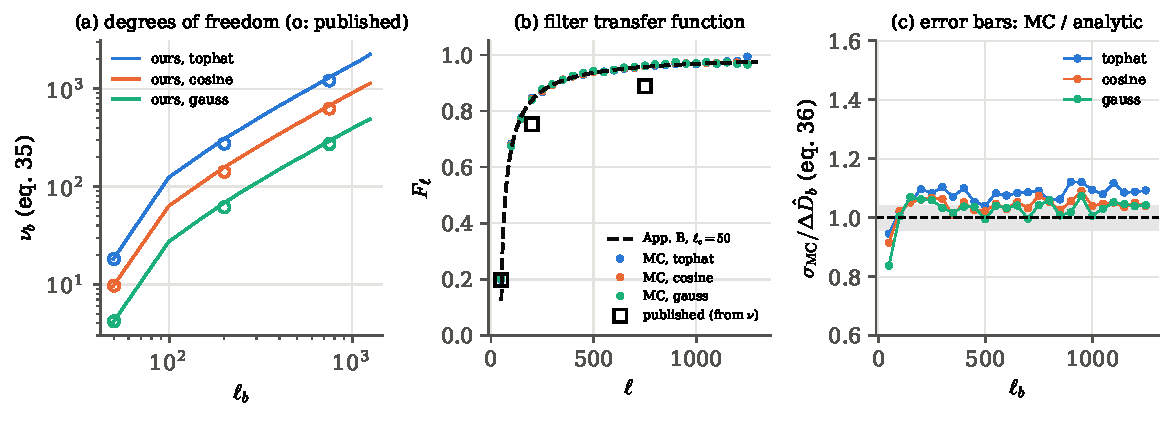
\includegraphics[width=12.5cm]{figures/ch08/boom_overlay.pdf}
\caption{Our Boomerang test against the published numbers. (a) Degrees of freedom $\nu_b$ of
\srcref{Hivon}{(35)} for the three weightings (lines) and the nine published values of their Fig.~6
(circles). (b) The transfer function: our simulated $F_b$ (dots), the parallel-scan formula
\eqref{8b:eq:B15} (dashed), and the values implied by the published $\nu$ (squares). (c) The simulated
error bars divided by the analytic ones of \srcref{Hivon}{(36)}; the grey band is the Monte Carlo error.}
\label{8b:fig:boom-overlay}
\end{figure}

\paragraph{The degrees of freedom (their Fig.~6).}
Inserting our $F$ into \eqref{8b:eq:hivon-nu} gives our $\nu$ for the three weightings at $\ell=50$, $200$ and
$750$ (\cref{8b:fig:boom-overlay}a, \cref{8b:tab:literature}). Above $\ell=50$ ours are larger, and the difference is
the ratio of the two transfer functions and nothing else:
$\EightBboomNuTopTwohundred/274.6=1.12=\EightBboomFTwohundred/\EightBboomFpubTwohundred$. A sharper check of their table is internal.
In \eqref{8b:eq:hivon-nu} only $w_2^2/w_4$ changes between weightings, so multiplying their top-hat $\nu$ by our
ratios of $w_2^2/w_4$ should give their cosine and Gaussian values. It does, to within $1\%$.

\paragraph{The binned kernel (their Fig.~3).}
\Cref{8b:fig:boom-kernel} shows the diagonal and two rows of $K_{bb'}$ and of its inverse for the top-hat
window, in the format of their figure. The diagonal is $\EightBboomKdiagTwo$ at $\ell_b=200$ and falls to
$\EightBboomKdiagTwelve$ at $1200$, the beam, pixel window and $\fsky w_2$ in one number; the rows fall by four to six
decades within a few hundred multipoles, and the inverse has the long negative wings of a deconvolution,
as in their figure.

\begin{figure}[htbp]
\centering
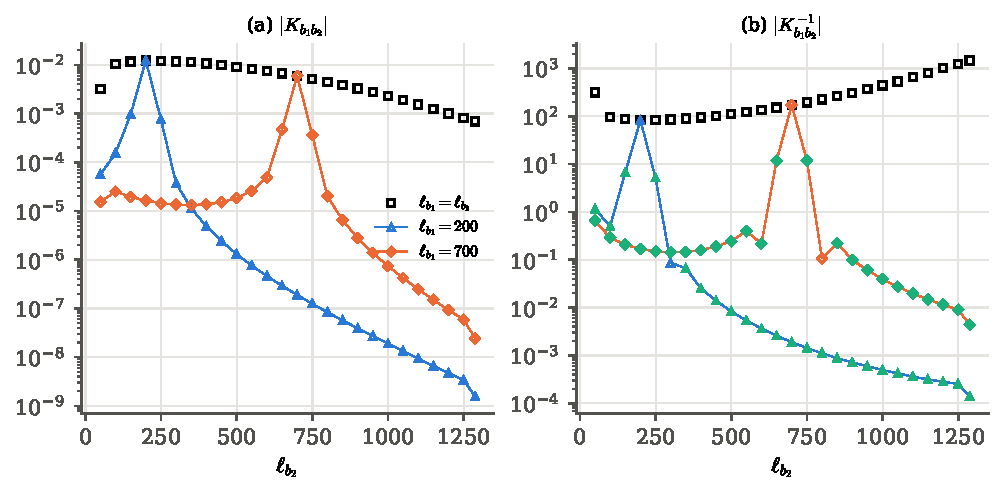
\includegraphics[width=12cm]{figures/ch08/boom_kernel.pdf}
\caption{The binned coupling kernel of the top-hat ellipse ($\fsky=1.8\%$, $\Delta\ell=50$), in the format of
Hivon et al.'s Fig.~3. (a) $|K_{b_1b_2}|$: the diagonal (squares) and the rows $\ell_{b_1}=200$ and $700$.
(b) $|K^{-1}_{b_1b_2}|$; green marks negative elements.}
\label{8b:fig:boom-kernel}
\end{figure}

\paragraph{The recovered spectrum and its error bars (their Fig.~5): what they claimed.}
They found the mean of $1352$ MASTER estimates ``in perfect agreement (to an error on the mean)'' with the
bin-averaged input, and the simulated error bars ``almost identical'' to the analytic error bar
\eqref{8b:eq:hivon-nu} \srcref{Hivon}{§4.2}; off-diagonal correlations were ``at most $10\%$''.

\paragraph{How we test it.}
For the error bar we divide the simulated scatter of $\widehat D_b$ by the square root of \eqref{8b:eq:hivon-nu}.
For the mean we use \emph{pulls}, as in \cref{8b:sec:coupling-check}: the mean of our estimates in a bin,
minus its prediction, divided by the Monte Carlo error of that mean (the scatter of single estimates
over $\sqrt{\EightBboomNsn}$). If the prediction is right, the pulls are draws of a standard Gaussian, and the
largest of $\EightBboomNbins$ should be about two, rarely above three. Two predictions are possible: the plain
bin average of the input, as in the paper, or the bandpower-window prediction \eqref{8b:eq:bpw}. The
numbers for the three weightings are in \cref{8b:tab:literature} and \cref{8b:fig:boom-overlay}c,
\cref{8b:fig:boom-spectrum}. In short: the analytic error bar is a few per cent optimistic in most bins and
pessimistic in the first; the mean agrees with the window prediction, with pulls larger than
chance until the errors shared by all skies are counted; against the plain bin average it is off by up to a third of a single sky's error bar; and the
top-hat's largest correlation exceeds $10\%$.

\paragraph{Why they differ.}
\emph{The error bar is a few per cent too small.} Equation \eqref{8b:eq:hivon-nu} counts modes, which gives the
variance of an optimal estimate. MASTER is not optimal, and its deconvolution amplifies the scatter
(\cref{8b:sec:quick}); a $5\%$ excess, against a Monte Carlo error of $2\%$, is invisible at the precision
of ``almost identical''.

\emph{In the first bin it is too large.} The bin $\ell=25$--$74$ contains a steep rise of both $D_\ell$ and $F_\ell$,
and the rule evaluates them at the bin's centre. That is step~3 of \eqref{8a:eq:hivon16}, which failed in
the full sky's first bin for the same reason (\cref{8a:sec:lit-hivon}).

\emph{The pulls against the windows are larger than chance.} All $\EightBboomNsn$ estimates share two
things measured from smaller sets. They are deconvolved with the same $F$, measured from only $\EightBboomNs$ skies.
Since $\widehat D_b\propto1/F_b$, a relative error $\delta$ of $F_b$ shifts every estimate by the same $-\delta D_b$.
And the same noise power, measured from only $\EightBboomNn$ noise-only skies, is subtracted from every one of
them, so its error shifts them all alike too. Averaging over $\EightBboomNsn$ skies shrinks their
independent scatter by $\sqrt{\EightBboomNsn}$ but leaves the common shifts untouched, so in units of the
Monte Carlo error of the mean they are magnified. For the top-hat, the scatter of $F$ between the six chunks of the
noise-free set gives common shifts of up to $\EightBboomPullFTop$ such errors, and the noise power up to
$\EightBboomPullNTop$, largest in the noise-dominated bins at high $\ell$. Adding both to the error of the mean, the
largest pulls become $\EightBboomPullTotTop$, $\EightBboomPullTotCos$ and $\EightBboomPullTotGau$ for the three weightings: about
what chance gives, since the largest of $\EightBboomNbins$ standard normal numbers is typically about $2$.

\emph{The plain bin average is the wrong prediction.} The offsets from it sit in the first bin, where
$D_\ell$ and $F_\ell$ rise steeply and the bandpower window differs from a flat average by $7\%$, and at the
peaks and troughs; the bandpower windows account for them (the pitfall of \cref{8b:sec:binning}). At
the resolution of their Fig.~5 such offsets are invisible; with $1350$ simulations they are measurable.

\emph{The top-hat correlates more.} Beyond the first three bins the correlation matrix
(\cref{8b:fig:boom-spectrum}b) is diagonal-dominated, but the top-hat's largest off-diagonal correlation
slightly exceeds their $10\%$. It has the sharpest edge, and so the longest leakage tail.

\begin{figure}[htbp]
\centering
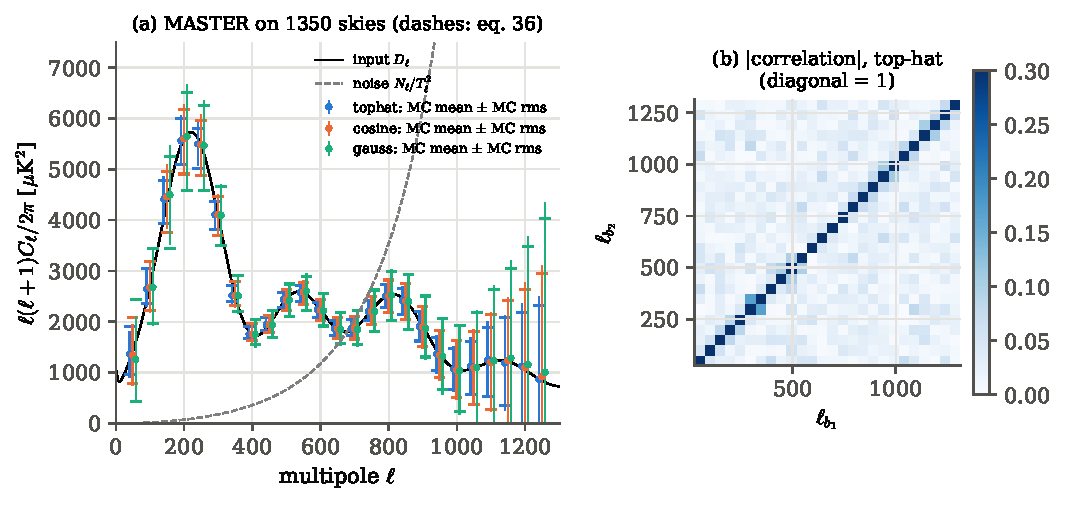
\includegraphics[width=12.5cm]{figures/ch08/boom_spectrum.pdf}
\caption{MASTER on $\EightBboomNsn$ simulated Boomerang-like skies, in the format of Hivon et al.'s Fig.~5.
(a) Mean and scatter of the estimates for the three weightings (slightly offset in $\ell$), the input
spectrum (black), the analytic error bars of \srcref{Hivon}{(36)} (dashes) and the noise on the sky
(grey dashed). (b) Absolute correlation matrix of the top-hat bandpowers.}
\label{8b:fig:boom-spectrum}
\end{figure}

\paragraph{The shape of the distribution (their Fig.~6).}
Their last test compared the histogram of the estimates in the bins at $\ell=50$, $200$ and $750$ with a
$\chi^2_\nu$ with the $\nu$ of \eqref{8b:eq:hivon-nu}, with no free parameter, and with a Gaussian of the same mean
and variance. \Cref{8b:fig:boom-hist} is the same figure from our simulations. At $\ell=50$, where $\nu$ is $18$,
$10$ and $4$, the histograms are skewed and the $\chi^2_\nu$ follows them where the Gaussian does not, most
clearly for the Gaussian weighting with $\nu\approx4$; at $\ell=200$ and $750$ the two models coincide. Their
conclusion carries over unchanged: for small sky coverage the likelihood of a low-$\ell$ bandpower must
be modelled as a $\chi^2$, not as a Gaussian \srcref{Hivon}{(37)}.

\begin{figure}[htbp]
\centering
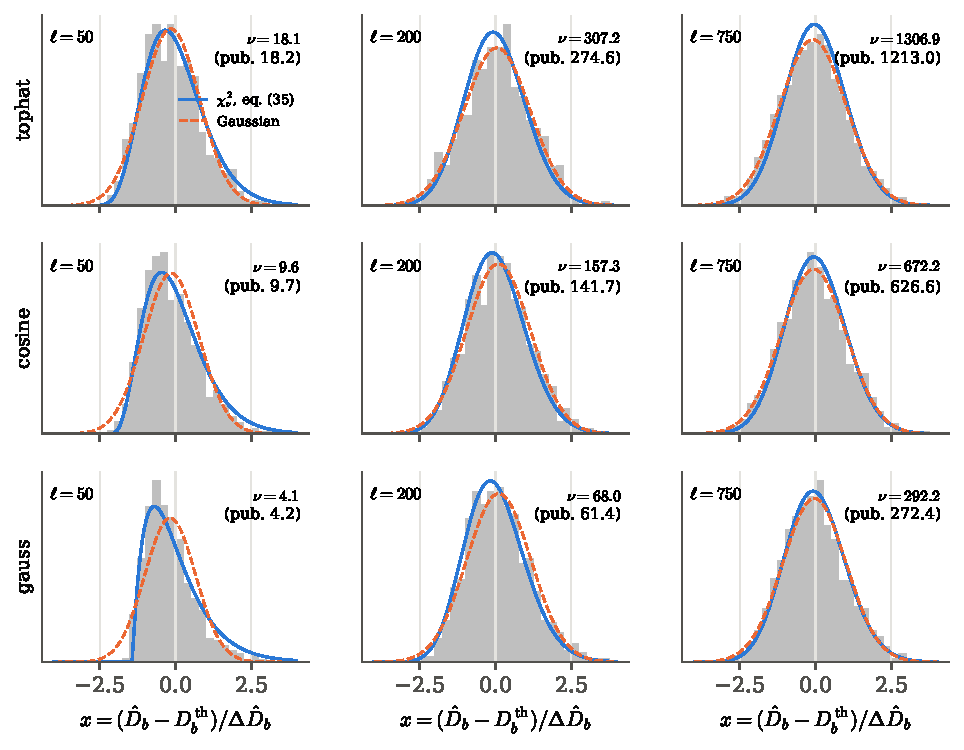
\includegraphics[width=11.5cm]{figures/ch08/boom_hist.pdf}
\caption{Distributions of the MASTER estimates, centred on the input and divided by the analytic error,
at $\ell=50$, $200$ and $750$ (columns) for the three weightings (rows), as in Hivon et al.'s Fig.~6. Blue: the
$\chi^2_\nu$ of eq.~(35) with our $\nu$ (their published $\nu$ in brackets); orange dashed: a Gaussian of the same
mean and variance.}
\label{8b:fig:boom-hist}
\end{figure}

\paragraph{Lesson.}
At the resolution of the paper's figures MASTER passes every test; with the same number of
simulations, read as numbers, each few-per-cent residual becomes measurable and has a cause we can
name: a non-optimal estimator, a transfer function measured once and shared by every estimate, and a
theory that must be passed through the bandpower windows.

\subsection{Efstathiou (2004), Hartlap et al.\ (2007), Taylor et al.\ (2013), NaMaster}
\label{8b:sec:lit-others}

\paragraph{Efstathiou.}
\emph{His question:} through a Galactic cut, can a cheap pseudo-$\Cell$ estimator be nearly as good as exact
maximum likelihood, and can its covariance be computed without simulations? \emph{His equations, here:}
the coupling matrix (his eqs.~9--11) is \eqref{8b:eq:Mdef}, with his symmetric $G_{\ell\ell'}=M_{\ell\ell'}/(2\ell'+1)$ and
his $\Xi(\ell,\ell',\mathcal W)$ ours; the exact covariance (his 14, 18) is \eqref{8b:eq:cov-exact}; the approximation
(15a) is \eqref{8b:eq:efstathiou}, with his $W^{(2)}$ the spectrum $\mathcal W^{(2)}$ of the squared window. \emph{What we
ran:} the $\EightBNsim$ skies through a $\pm20^\circ$ band, the exact band covariance from the ring sum
\eqref{8b:eq:K-ring}, and the approximation against both. His Fig.~1 (the mean pseudo-spectrum is the
input convolved with $M$, and the deconvolved estimate is unbiased) is our mean-square pull of
$\EightBpullchiBand$ (\cref{8b:sec:coupling-check}) and the unbiased MASTER of \cref{8b:sec:binning}; his Fig.~4
(exact covariance against simulations) is our ratio $\EightBexactMCmean\pm\EightBexactMCrms$, the Monte Carlo precision.
\emph{The difference:} his approximation is accurate at $\ell\gtrsim20$ and wrong by up to $25\%$ at $\ell=2$; ours is wrong
by $43\%$ at $\ell=2$ and $10\%$ at $\ell=20$. His cut of $\pm10^\circ$ removes $\sin10^\circ=17\%$ of the sky, ours $\sin20^\circ=34\%$,
twice as much; the wider cut widens the coupling kernel, and the approximation, which assumes the
spectrum constant across the kernel, fails further up in $\ell$. \emph{Lesson:} the approximation is a
high-$\ell$ tool, and the multipole where it becomes good moves up with the cut.

\paragraph{Hartlap et al.}
\emph{Their question:} when a covariance is estimated from $n$ simulations and inverted, is the inverse
unbiased, and if not, by how much? \emph{Their equation, here:} the factor $(n-p-2)/(n-1)$ of their eq.~17 is
derived in \eqref{8b:eq:hartlap-derived}; their $n$ and $p$ (simulations and data points) are ours, and their
debiased inverse is our $\Psi$. \emph{What we ran:} their Fig.~1 test, $n=60$, $p_1=240$, three covariance models,
with $\EightBhartlapRep$ repetitions instead of $10^4$ (\cref{8b:fig:hartlap}a). \emph{Side by side:} the raw
trace ratio follows $(n-p-2)/(n-1)$ and the corrected one is one to within $\EightBhartlapCorWorst$. There is no
difference to explain beyond the Monte Carlo noise. \emph{Lesson:} the factor is exact for Gaussian
vectors, and it holds for skewed CMB bandpowers too (\cref{8b:sec:hartlap-test}).

\paragraph{Taylor et al.}
\emph{Their question:} once the precision matrix is unbiased, how noisy is the error bar it gives, and how
many simulations does a target precision need? \emph{Their equations:} $\varepsilon=\sqrt{2/(N_S-N_D-4)}$ (their eq.~55) and
the planning rule \eqref{8b:eq:taylor} (their eq.~58), with their $N_S$, $N_D$ our $n$, $p$. \emph{What we ran:} the
one-parameter amplitude fit of \cref{8b:sec:taylor}, $\EightBNall$ times for each $n$. \emph{Side by side:} at
$N_S=40$ the scatter of $\widehat{\sigma^2_A}$ is $\EightBtaylorScatForty$, against $\EightBtaylorPredForty$ from their eq.~(55) and $0.43$ from
the exact \eqref{8b:eq:sigA}. \emph{The difference:} their formula is the relative scatter of the Fisher
information, an inverse $\chi^2_{n-p}$, and the ``$-4$'' is that distribution's long tail; the variance itself is a
$\chi^2_{n-p}$ and scatters as $\sqrt{2/(n-p)}$, smaller at small $n-p$ (\cref{8b:sec:taylor}). \emph{Lesson:} their rule
errs on the safe side; it asks for $\EightBtaylorFivePct$ simulations for $5\%$ error bars on our $\EightBpcov$ bins.

\paragraph{NaMaster, in words.}
NaMaster is the standard pseudo-$\Cell$ code of current surveys \cite{Alonso2019}, and the question for us
is whether it computes what we derived. Its conventions map onto
ours one to one. Its mode-coupling matrix for two spin-0 fields with masks $v$ and $w$ is
$M^{00}_{\ell\ell'}=\frac{2\ell'+1}{4\pi}\sum_{\ell''}P^{vw}_{\ell''}(\ell\;\ell'\;\ell'';0\;0\;0)^2$ with
$P^{vw}_{\ell''}=(2\ell''+1)\,\mathrm{PCL}_{\ell''}(v,w)$ \cite[eq.~12]{Alonso2019}, which for $v=w=W$ is our
\eqref{8b:eq:Mdef}. Its bandpowers are weighted sums of the coupled pseudo-$\Cell$ over the multipoles of
each band, with weights normalised to one; the binned coupling matrix is inverted, and theory is
compared with data only through the bandpower windows $\mathcal F_{q\ell}$ \cite[eqs~15--19]{Alonso2019}, our
\eqref{8b:eq:bpw}. The default weights are flat in $\Cell$; Hivon's flat-in-$D_\ell$ binning corresponds to
weights proportional to $\ell(\ell+1)$. Beyond what we use, it handles spin-2 fields (polarisation, shear) with
$E/B$ purification, and deprojects foreground templates with the corresponding bias correction. NaMaster
is not installed in our environment, so the comparison is with its published equations, not with its
output.

\begin{table}[htbp]
\centering
\small
\renewcommand{\arraystretch}{1.22}
\begin{tabular}{@{}>{\raggedright\arraybackslash}p{3.7cm}>{\raggedright\arraybackslash}p{2.5cm}>{\raggedright\arraybackslash}p{2.7cm}>{\raggedright\arraybackslash}p{3.4cm}@{}}
\toprule
quantity & published & ours & why they differ \\
\midrule
\multicolumn{4}{@{}l}{\emph{Hivon et al.\ (2002), Boomerang test}}\\
$\fsky$ of the ellipse & $1.82\%$ & $\EightBboomFsky\%$ & --- \\
$w_2^2/w_4$: top-hat, cosine, Gaussian & $1$, $0.514$, $0.223$ & $\EightBboomWTop$, $\EightBboomWCos$, $\EightBboomWGau$ & --- \\
$F$ at $\ell=50$, $200$, $750$ & $\EightBboomFpubFifty$, $\EightBboomFpubTwohundred$, $\EightBboomFpubSevenfifty$ (from $\nu$) & $\EightBboomFFifty$, $\EightBboomFTwohundred$, $\EightBboomFSevenfifty$ (eq.~B15: $\EightBboomFbfifteenFifty$, $\EightBboomFbfifteenTwohundred$, $\EightBboomFbfifteenSevenfifty$) & real scans vs ideal parallel scans \\
$\nu$, top-hat, $\ell=50,200,750$ & $18.2$, $274.6$, $1213$ & $\EightBboomNuTopFifty$, $\EightBboomNuTopTwohundred$, $\EightBboomNuTopSevenfifty$ & ratio of the $F$'s \\
$\nu$, cosine & $9.7$, $141.7$, $626.6$ & $\EightBboomNuCosFifty$, $\EightBboomNuCosTwohundred$, $\EightBboomNuCosSevenfifty$ & ratio of the $F$'s \\
$\nu$, Gaussian & $4.2$, $61.4$, $272.4$ & $\EightBboomNuGauFifty$, $\EightBboomNuGauTwohundred$, $\EightBboomNuGauSevenfifty$ & ratio of the $F$'s \\
their cosine $\nu$ from their top-hat $\nu$ & $9.7$, $141.7$, $626.6$ & $\EightBboomNuPredCosFifty$, $\EightBboomNuPredCosTwohundred$, $\EightBboomNuPredCosSevenfifty$ & --- \\
their Gaussian $\nu$ from their top-hat $\nu$ & $4.2$, $61.4$, $272.4$ & $\EightBboomNuPredGauFifty$, $\EightBboomNuPredGauTwohundred$, $\EightBboomNuPredGauSevenfifty$ & --- \\
$\delta F/F$ coefficient $a$, eq.~(38) & $0.6$--$0.9$ & $\EightBboomA\pm\EightBboomAErr$ (counting: $0.52$) & mask couples the bins \\
MC / analytic error, eq.~(36), median & ``almost identical'' & $\EightBboomRatioTop$, $\EightBboomRatioCos$, $\EightBboomRatioGau$ & MASTER not optimal \\
the same, first bin & --- & $\EightBboomRatioLowTop$, $\EightBboomRatioLowCos$, $\EightBboomRatioLowGau$ & $D_\ell$, $F_\ell$ steep in the bin \\
largest pull of the mean vs windows & none & $\EightBboomPullWinTop$, $\EightBboomPullWinCos$, $\EightBboomPullWinGau$ & common errors of $F$ and of the noise; with them, $\EightBboomPullTotTop$, $\EightBboomPullTotCos$, $\EightBboomPullTotGau$ \\
largest offset vs plain bin average, in single-sky $\sigma$ & none & $\EightBboomBiasSigTop$, $\EightBboomBiasSigCos$, $\EightBboomBiasSigGau$ & bandpower windows \\
largest off-diagonal correlation & $\le10\%$ & $\EightBboomOffTop$, $\EightBboomOffCos$, $\EightBboomOffGau\%$ & sharp top-hat edge \\
low-$\ell$ shape & $\chi^2_\nu$, not Gaussian & same & --- \\
simulations & $450+250+1350$ & $\EightBboomNn+\EightBboomNs+\EightBboomNsn$ & maps, not timestreams \\
\midrule
\multicolumn{4}{@{}l}{\emph{Efstathiou (2004)}}\\
approximation (15a), $\ell=2$ & $\le25\%$ off ($\pm10^\circ$) & $\EightBexactApproxTwo$ ($\pm20^\circ$) & wider cut \\
approximation (15a), $\ell\gtrsim20$ & accurate & $\EightBexactApproxTwenty$ at $20$, $\EightBexactApproxForty$ at $40$ & --- \\
exact (18) vs simulations & ``almost perfect'' & $\EightBexactMCmean\pm\EightBexactMCrms$ & --- \\
$M$ invertible & cuts $\lesssim30^\circ$ & band yes, caps $<50\%$ no & pair-separation rule \\
\midrule
\multicolumn{4}{@{}l}{\emph{Hartlap et al.\ (2007); Taylor et al.\ (2013)}}\\
raw trace ratio, $n=60$, $p=40$ & $(n-p-2)/(n-1)=0.305$ & $\EightBhartlapRawForty$ & --- \\
corrected ratio & $1$ & $1\pm\EightBhartlapCorWorst$ & --- \\
scatter of $\sigma^2_A$, $N_S=40$ & $\EightBtaylorPredForty$ (eq.~55) & $\EightBtaylorScatForty$ & ``$-4$'': scatter of the information, not of the variance \\
$N_S$ for $5\%$ errors, $N_D=\EightBpcov$ & $200+N_D+4$ & $\EightBtaylorFivePct$ & --- \\
\bottomrule
\end{tabular}
\caption{Published cut-sky results and the same quantities from our code. Where three values are
given for the Boomerang test they are for the top-hat, cosine and Gaussian weightings.}
\label{8b:tab:literature}
\end{table}
\section{How it is done in research}
\label{8b:sec:research}

A real temperature analysis has one sky and a stack of simulations. Everything it publishes about the
spectrum, from the error bar of a single bandpower to the claim that no systematic effect is left,
is a statement about how the estimator behaves on simulated skies that went through the same mask
and the same code as the data. The order in which a full-sky analysis runs (maps, spectra,
deconvolution, covariance, likelihood, checks) was laid out in \cref{8a:sec:research}. The mask
changes what each of those steps has to do, and a real analysis makes a definite choice at each
one. Seeing those choices once, and then running a small analysis that makes the same ones on a
laptop, ties together the pieces of this chapter.

\subsection{The cut-sky choices of a real analysis}
\label{8b:sec:research-choices}

The reference here is the Planck 2018 high-$\ell$ temperature likelihood \cite{Planck2018V}, which is a
pseudo-$\Cell$ analysis of exactly the kind built in \cref{8b:sec:masks,8b:sec:coupling,8b:sec:master}.

\paragraph{The mask.}
A Galactic mask is made by thresholding a map of foreground emission, so that it follows the dust
and not a straight line of latitude, and it is multiplied by masks of point sources, of carbon
monoxide line emission and of extended objects, each specific to the frequency of the map. Planck
keeps $66\%$, $57\%$ and $47\%$ of the sky at $100$, $143$ and $217$\,GHz (the masks T66, T57 and T47), because
dust is brighter at the higher frequency. The Galactic part is apodised with a Gaussian of $4.71^\circ$
full width at half maximum and the point-source holes with one of $30'$ \cite[§3.2]{Planck2018V}. The
reason given is the one of \cref{8b:sec:apodisation}: a soft edge confines the coupling to neighbouring
multipoles and makes the bandpowers less correlated. The price is the one we computed there in modes:
the apodisation removes about $10\%$ of the effective sky fraction \cite[§3.2]{Planck2018V}.

\paragraph{The coupling and the bandpowers.}
The coupling matrix of each mask is computed exactly from the mask's own spectrum, as in
\eqref{8b:eq:Mdef}, and inverted in bins. The bins are $\Delta\ell=5$ for $30\le\ell\le99$, $9$ up to $\ell=1503$,
$17$ up to $2013$ and $33$ up to $2508$ \cite[§3.2.5]{Planck2018V}. They are narrow because a $60\%$
mask couples multipoles over only a few $\ell$ (\cref{8b:fig:coupling-columns}); they widen at high $\ell$
because there the noise, not the coupling, sets the useful resolution. The spectra are cross-spectra
between the two half-missions and between detector sets, so that no noise bias enters
(\cref{8a:sec:cross}).

\paragraph{The covariance.}
Planck does not estimate its covariance from simulations. With hundreds of bandpowers for each of
several cross-spectra, \eqref{8b:eq:taylor} would demand thousands of end-to-end simulations, and only
$300$ exist. The covariance is computed analytically for a fiducial model, with the large Galactic
mask treated by the MASTER-type expressions of \cref{8b:sec:quick} (the approximation that Efstathiou
derived), the point-source masks by a correction measured on Monte Carlo simulations, and the
anisotropy of the noise by a heuristic correction \cite[§3.1]{Planck2018V}. The $300$ FFP10 end-to-end
simulations are used to test the result \cite{Planck2018V}.

\paragraph{The likelihood and the checks.}
Above $\ell=30$ the bandpowers enter a Gaussian likelihood, $-2\ln\Like=(\hat{\bm C}-\bm C(\params))\T\Sigma^{-1}(\hat{\bm C}-\bm C(\params))$,
with the covariance $\Sigma$ fixed at the fiducial model. The Gaussian shape is a choice justified by the
central limit theorem, and its symmetry causes a small bias for $30\le\ell<100$
\cite[§3.1]{Planck2018V}, which is the skewness of \cref{8b:sec:shape-cut} seen from the likelihood side.
Its size follows from the mode count \eqref{8b:eq:hivon-count}. A bin of five multipoles at $\ell=50$ on about
$60\%$ of the sky holds $\nu\approx(2\times50+1)\times5\times0.6\approx300$ modes, so the scaled $\chi^2$ has skewness
$\sqrt{8/\nu}\approx0.16$; at $\ell=30$, $\nu\approx180$ and the skewness is $0.21$. Small, but not zero, and it is the
multipole range where a symmetric likelihood errs most; above $\ell=100$ the bins are wider and the
skewness falls below $0.1$.

Null tests difference half-missions, detector sets, and odd and even rings of the scan, so that the
sky cancels and only noise and systematics remain. The logic is that of \cref{4a:sec:null}: we assume
the difference is noise alone, because for that case the simulations give us its distribution; and we
ask whether a result like the observed one, or one further in the same direction, would be
unremarkable if that were true. The probability of such a result is the probability to exceed (PTE)
under the simulations \cite{Planck2018V}; the null-test example of \cref{8b:sec:research-run} works one
through.
Ground-based experiments such as ACT and SPT map patches of a few to a few tens of percent of the sky,
filter their timestreams, and so add the transfer function of \cref{8b:sec:transfer}, measured on
noise-free simulations; in every other respect their spectra are built the same way.

\begin{figure}[htbp]
\centering
\begin{tikzpicture}[
  bx/.style={draw=accent,thick,rounded corners=2pt,fill=ideabg,font=\small,
             minimum height=10mm,align=center,text width=25mm},
  sb/.style={bx,draw=tangentgreen!80!black},
  nb/.style={bx,draw=bdryred!80!black},
  flow/.style={->,thick,accent}]
  \node[bx] (map)  at (0,0)    {two half-mission\\ maps $d_1$, $d_2$};
  \node[bx] (mask) at (0,-2.2) {window $W$:\\ band $\times$ holes};
  \node[bx] (M)    at (3.6,-2.2) {$\mathcal W_\ell\to M_{\ell\ell'}$\\ (3$j$ symbols)};
  \node[bx] (pcl)  at (3.6,0)  {pseudo cross-\\ spectrum $\widetilde C^{12}_\ell$};
  \node[bx] (Db)   at (7.2,0)  {MASTER\\ $\widehat D_b=K^{-1}P\widetilde C^{12}$};
  \node[sb] (sims) at (7.2,-2.2) {$n$ simulations\\ through the chain};
  \node[sb] (cov)  at (10.8,-2.2) {$\widehat\Cmat$, Hartlap\\ $\Psi$};
  \node[nb] (null) at (10.8,-4.4) {null test on\\ $(d_1-d_2)/2$};
  \node[bx] (like) at (10.8,0) {likelihood\\ $\hat A\pm\sigma_A$};
  \draw[flow] (map) -- (pcl);
  \draw[flow] (mask) -- (M);
  \draw[flow] (mask.north) -- (map.south);
  \draw[flow] (M) -- (Db);
  \draw[flow] (pcl) -- (Db);
  \draw[flow] (Db) -- (like);
  \draw[flow] (sims) -- (cov);
  \draw[flow] (cov) -- (like);
  \draw[flow] (cov) -- (null);
  \draw[flow,dashed] (Db.south) -- (sims.north);
\end{tikzpicture}
\caption{The cut-sky analysis as it runs. The window enters twice: it multiplies the maps and, through
its spectrum alone, fixes the coupling matrix. The simulations (green) pass through the same chain as the
data (the dashed arrow) and supply what no formula gives here: the covariance, its inverse and the
distribution of the null test (red).}
\label{8b:fig:pipeline-flow}
\end{figure}

\subsection{Our pipeline, end to end}
\label{8b:sec:research-run}

\paragraph{The setting.}
The script \pyname{31_pipeline.py} runs the whole chain of \cref{8b:fig:pipeline-flow} once, on a sky
whose random seed is kept apart from those of the simulations, so that it plays the part of the data.
The instrument is the toy experiment of \cref{8a:sec:model}: $N_{\rm side}=256$, a $30'$ Gaussian beam and white
noise of $200\,\mu$K\,arcmin. The data are two half-mission maps of the same sky, each with noise $\sqrt2$
larger, so that their average has the noise of the full experiment. The window is the product of a
Galactic band, $|b|<20^\circ$ with a $5^\circ$ cosine taper, and $400$ randomly placed point-source holes of radius
$1^\circ$, now themselves given a $1^\circ$ taper (the band and the holes of \cref{8b:sec:window}, multiplied together). It keeps $\fsky=\EightBpipeFsky$ of the sky with
$w_2=\EightBpipeWtwo$. The questions are the ones a real analysis answers: what is the spectrum, how
uncertain is it, is anything in the data that is not sky, and what amplitude of the fiducial spectrum
does the data prefer?

\pyfile[firstline=77,lastline=94]{code/ch08/31_pipeline.py}{One observation and its bandpowers}

\paragraph{The code.}
\pyname{observe} draws one Gaussian sky from the fiducial spectrum, smooths it with the beam and pixel
window, and adds two independent noise maps; the optional stripes are the systematic used below.
\pyname{bandpowers} multiplies both maps by the window, transforms them, and forms two spectra: the cross
spectrum of the halves and the spectrum of their half-difference, in which the sky cancels. Both are
binned with $P$ (bins of $20$) and deconvolved with $K^{-1}$, the binned coupling of
\eqref{8b:eq:bpw}'s definition with $F_\ell=1$ (no filter) and $T_\ell^2$ the beam and pixel window. The
coupling matrix is computed once from the window's spectrum, and the same two functions run on the data
and on each of the $\EightBpipeNsim$ simulations. The bandpowers used are the $p=\EightBpipeNbins$ bins with
$\EightBpipeLlo\le\ell\le\EightBpipeLhi$.

\begin{figure}[htbp]
\centering
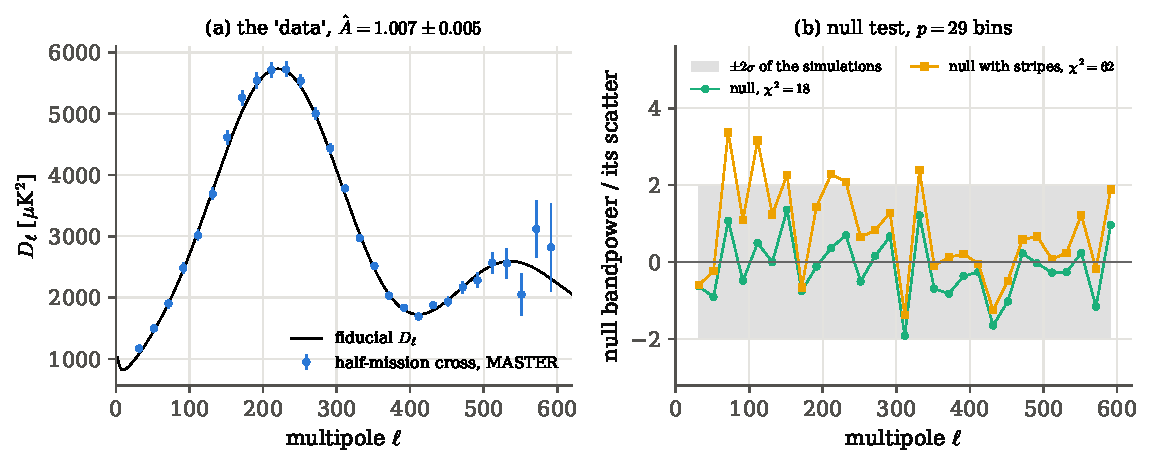
\includegraphics[width=\linewidth]{figures/ch08/pipeline.pdf}
\caption{(a) The ``data'': MASTER bandpowers of the half-mission cross spectrum through the band-and-holes
window, with error bars from the simulations, on the fiducial spectrum. (b) The null spectrum of the
half-difference map, minus its simulated mean and divided by its simulated scatter, without (green) and with
(orange) a $3\,\mu$K ring-striping systematic in the second half. The stripes add power, so almost every
orange point sits above its green partner, most of all below $\ell\approx350$; which orange points leave the
grey band, and by how much, changes from one draw to the next.}
\label{8b:fig:pipeline}
\end{figure}

\paragraph{The covariance and its inverse.}
The covariance of the $p=\EightBpipeP$ bandpowers is the sample covariance of the $n=\EightBpipeNsim$
simulations, and its inverse is corrected by the Hartlap factor of \cref{8b:sec:hartlap}:
\begin{align*}
  \Psi=\frac{n-p-2}{n-1}\,\widehat\Cmat^{-1}
  \eqby{1}\frac{400-29-2}{400-1}\,\widehat\Cmat^{-1}
  \eqby{2}0.925\,\widehat\Cmat^{-1}.
\end{align*}
\begin{explain}
  \item $n=\EightBpipeNsim$ simulations and $p=\EightBpipeP$ bins.
  \item $369/399=0.9248$, the script's $\EightBpipeHartlap$.
\end{explain}
Without the factor every $\chi^2$ would be $8\%$ too large and every error bar $4\%$ too small. With it,
the variance of a single parameter is still uncertain by $\sqrt{2/(n-p)}=\sqrt{2/371}=7.3\%$ by
\eqref{8b:eq:sigA}, its error bar by $3.7\%$, and biased high by $(n-p)/(n-p-2)-1=0.5\%$. Those are the
cost of $400$ simulations.

\paragraph{Example: the amplitude and its error bar.}
The simplest physics question is how much CMB power there is relative to the fiducial model. Write the
model for the bandpowers as $\bm D=A\bm t$, with $\bm t$ the fiducial bandpowers $P_{b\ell}\Cell^{\rm fid}$ and $A$ a free
amplitude, and the Gaussian likelihood with the precision matrix $\Psi$:
\begin{align*}
  -2\ln\Like(A)&\eqby{1}(\widehat{\bm D}-A\bm t)\T\Psi(\widehat{\bm D}-A\bm t)+\text{const}\\
  &\eqby{2}A^2\,\bm t\T\Psi\bm t-2A\,\bm t\T\Psi\widehat{\bm D}+\widehat{\bm D}\T\Psi\widehat{\bm D}+\text{const}\\
  &\eqby{3}\frac{(A-\hat A)^2}{\sigma_A^2}+\text{const}',\qquad
  \hat A=\frac{\bm t\T\Psi\widehat{\bm D}}{\bm t\T\Psi\bm t},\quad \sigma_A^2=\frac1{\bm t\T\Psi\bm t}.
\end{align*}
\begin{explain}
  \item The Gaussian likelihood of the bandpowers, with the covariance fixed (it does not depend on $A$).
  \item Expand the quadratic form; $\Psi$ is symmetric, so the two cross terms are equal.
  \item Complete the square in $A$; everything without $A$ goes into the constant.
\end{explain}
The likelihood in $A$ is exactly Gaussian, with its peak at a weighted average of the bin-by-bin
ratios $\widehat D_b/t_b$ and its width given by the Fisher information $\bm t\T\Psi\bm t$ (\cref{ch:10}).
Because $\hat A$ is linear in $\widehat{\bm D}$ and MASTER is unbiased, $\hat A$ is unbiased whatever $\Psi$ is; the
precision matrix only sets the weights, and a noisy one gives slightly suboptimal weights, not a bias.
On the data $\hat A=\EightBpipeA\pm\EightBpipesA$. Run on each simulation, the same estimator has mean
$\EightBpipeAsimMean$ and standard deviation $\EightBpipeAsimStd$, which matches the Fisher width, and the interval
$\hat A\pm\sigma_A$ covers the input $A=1$ in $\EightBpipeCover\%$ of the simulations, as a $68\%$ interval should. The
data sit within two standard deviations of the input, and the fit has $\chi^2=\EightBpipeChiFit$ for $p-1=28$ degrees of
freedom (PTE $\EightBpipePTEFit$): one amplitude describes all $29$ bins.

\paragraph{Example: a null test, and what could have produced its value.}
\emph{The event.} The half-difference map $(d_1-d_2)/2$ contains the noise of the two halves and no sky.
Its bandpowers, minus their mean over the simulations, give $\chi^2=\EightBpipeChiData$ with the precision
matrix $\Psi_{\rm null}$ of the simulated null spectra, for $p=29$ bins.
\emph{What could have produced it?} Two things: noise behaving as the simulations say, or noise plus
something the simulations do not contain (a drift, a stripe, a calibration change between halves).
\emph{How probable is the value under the first?} The simulations answer directly: the fraction of
simulated null spectra with a larger $\chi^2$ is the PTE, $\EightBpipePTE$ in this run. That is not small
enough to doubt the noise model, and the test passes. It is a test of the first hypothesis alone (\cref{ch:04}): a
small PTE would say that the noise model fails, not what replaced it.

To see the test fail, the script adds to the second half a pattern of the kind a scan can leave: a
random offset of $\EightBpipeSigSys\,\mu$K rms on every ring of constant latitude. Such a pattern $f(\theta)$ depends
only on the colatitude, so its coefficients are
$a_{\ell m}=\int f(\theta)\lambda_{\ell m}(\theta)\sin\theta\,\dd\theta\int_0^{2\pi}e^{-im\phi}\dd\phi$, and the $\phi$ integral vanishes for
every $m\neq0$. On the full sky all its power sits in the $m=0$ modes, a little at every $\ell$; the mask
spreads it to other $m$. The null $\chi^2$ becomes $\EightBpipeChiSys$, with PTE
$\EightBpipeChiSysLess\EightBpipePTESys$. \Cref{8b:fig:pipeline}b shows why a $\chi^2$ is the right summary. In this run the largest single excess is
$\EightBpipeSysMaxPull$ standard deviations, which a reader scanning $29$ bins might put down to bad luck. The
$\chi^2$ does better: it adds up the excess of every bin, the small ones as well as the large. Under
noise alone it is a $\chi^2_{29}$, with mean $29$, variance $2\times29=58$ and standard deviation $7.6$; the observed
value lies $(\EightBpipeChiSys-29)/7.6=\EightBpipeSysNsig$ standard deviations above the mean.
A second, cruder count looks only at signs: under noise alone each bin is as likely to sit above
zero as below, so the number of high bins is binomial with mean $14.5$ and standard deviation
$\sqrt{29/4}=2.7$. Here $\EightBpipeSysNhigh$ of the $29$ bins are high, and $\EightBpipeSysNhigh$ or more would
happen by chance with probability $p\EightBpipeSysPhighRel\EightBpipeSysPhigh$. The count throws away how far each
bin is from zero, so it is weaker than the $\chi^2$: stripes that push a few bins far up can leave it
unremarkable.
Is this one data set a lucky catch? The script repeats the test on $\EightBpipeNrep$ fresh data sets, each
with its own sky, noise and stripes. The null $\chi^2$ has median $\EightBpipeChiSysMed$, so stripes of this size
usually fail the test. But not always: the lowest of the $\EightBpipeNrep$, $\EightBpipeChiSysMin$, lies only
$\EightBpipeNsigSysMin$ standard deviations above the mean, a value noise alone reaches often enough that the
test could pass. A null test that passes does not prove the
data are clean; it says the contamination is not much larger than the noise.

\paragraph{Example: why the simulated $\chi^2$ values come out low.}
There is a subtlety in using the same simulations for the covariance and for the null distribution.
For the simulations themselves, with residuals $\bm r_i=\bm v_i-\bar{\bm v}$,
\begin{align*}
  \frac1n\sum_{i=1}^n\bm r_i\T\Psi\bm r_i
  &\eqby{1}\frac{n-p-2}{n(n-1)}\sum_i\operatorname{tr}\bigl(\widehat\Cmat^{-1}\bm r_i\bm r_i\T\bigr)\\
  &\eqby{2}\frac{n-p-2}{n(n-1)}\operatorname{tr}\bigl(\widehat\Cmat^{-1}(n-1)\widehat\Cmat\bigr)\\
  &\eqby{3}\frac{(n-p-2)\,p}{n}
  =\frac{369\times29}{400}=26.75 .
\end{align*}
\begin{explain}
  \item $\Psi=\frac{n-p-2}{n-1}\widehat\Cmat^{-1}$, and a number equals its own trace,
        $\bm r\T\mathsf A\bm r=\operatorname{tr}(\mathsf A\bm r\bm r\T)$.
  \item The sum of the outer products of the residuals is $(n-1)\widehat\Cmat$, by the definition of the
        sample covariance.
  \item $\operatorname{tr}\Id_p=p$.
\end{explain}
This is an identity, true for every set of simulations, and the script finds $\EightBpipeChiSimMean$ (scatter
$\EightBpipeChiSimStd$). An independent data vector $\bm d$ behaves differently, and three facts give its value.
\emph{The residual's covariance.} $\bm r=\bm d-\bar{\bm v}$, with $\bm d$ independent of the simulations; $\bm d$ has
covariance $\Cmat$ and the mean of $n$ simulations has $\Cmat/n$, so $\E[\bm r\bm r\T]=\Cmat(1+1/n)$.
\emph{Independence.} $\Psi$ is built from the simulations, so it is independent of $\bm d$; for Gaussian draws
the sample covariance is also independent of the sample mean $\bar{\bm v}$ (\cref{8b:sec:hartlap}), so $\Psi$ is
independent of $\bm r$ and the average of the product factorises.
\emph{Unbiasedness.} $\E[\Psi]=\Cmat^{-1}$, by \eqref{8b:eq:hartlap-derived} with the Hartlap factor. Then
\[
  \E[\bm r\T\Psi\bm r]=\E\operatorname{tr}(\Psi\bm r\bm r\T)=\operatorname{tr}\bigl(\E[\Psi]\,\E[\bm r\bm r\T]\bigr)
  =\operatorname{tr}\bigl(\Cmat^{-1}\Cmat(1+1/n)\bigr)=p\,(1+1/n)=29.07 .
\]
The simulations, by contrast, were used to build $\Psi$: each $\bm r_i$ helped make the covariance it is
measured against, and the identity above gives $26.75$. They fit their own covariance a little too
well, so the reference distribution sits about two units of $\chi^2$ low and the PTE of real data comes
out slightly too small. The test errs towards
failing, which is the safe side; a cleaner test keeps a separate set of simulations for the null
distribution.

\paragraph{What the laptop version leaves out.}
Each step of \cref{8b:fig:pipeline-flow} was reduced to fit on a laptop. Each reduction removes
something whose effect is either known or not the subject here, and each has a price.

\begin{taxonomy}[The cut-sky pipeline: research version and laptop version]
\small
\begin{tabular}{@{}>{\raggedright\arraybackslash}p{1.8cm}>{\raggedright\arraybackslash}p{3.9cm}>{\raggedright\arraybackslash}p{3.1cm}>{\raggedright\arraybackslash}p{3.5cm}@{}}
step & research version & here & cost of the reduction \\
\hline
maps & several frequencies, $N_{\rm side}=2048$, $\ell\le2508$, foregrounds & one channel, $N_{\rm side}=256$, CMB only, $\ell\le\EightBpipeLhi$ & no damping tail, no foreground model \\
mask & thresholded foreground maps, thousands of sources, T66--T47 per frequency & geometric band, $400$ random holes & same mathematics, not tied to real foregrounds \\
coupling & exact, from $\mathcal W_\ell$ to $2\ell_{\max}$ & the same & none \\
noise & anisotropic, correlated, from the scan & white, uniform, two halves & no anisotropic-noise correction \\
covariance & analytic for a fiducial model, Monte Carlo corrections, tested on $300$ end-to-end simulations & $\EightBpipeNsim$ Gaussian simulations, Hartlap factor & $7\%$ uncertainty on a parameter variance; no systematics in $\Cmat$ \\
null tests & half-missions, detector sets, odd/even rings, every frequency & one half-mission null, one injected systematic & tests only what we put in \\
likelihood & multi-frequency, foreground and instrument nuisance parameters & one amplitude & no degeneracies to marginalise \\
\end{tabular}
\end{taxonomy}

The reduction that matters most for the statistics is in the covariance. At $N_{\rm side}=2048$ and
$\ell_{\max}=2500$ each simulation costs about $(2048/256)^3\approx500$ times more than ours (the transform cost
grows as $N_{\rm pix}^{1/2}\ell_{\max}^2\propto N_{\rm side}^3$, \srcref{Hivon}{(30)}), and the data vector has hundreds of bins
per spectrum. That is why a research analysis models its covariance and uses the simulations to test
the model, while ours can afford to use the simulations directly. The structure is the same in both:
the same code on data and on simulations, and every statement about the data read off the
simulations.

\begin{inpractice}[The simulations as the instrument]
In \cref{ch:07} the simulations reproduced the $\chi^2_{2\ell+1}$ law and the cosmic variance, which were
known in advance: they \emph{verified} a formula, and agreement tested the code. In a cut-sky analysis the
same loop is the measuring \emph{instrument}. The transfer function of a filtered scan, the covariance
that enters the likelihood, the distribution of a null-test $\chi^2$ and the coverage of the final error
bars exist only as properties of the simulations. Planck, ACT and SPT all compute their spectra
with pseudo-$\Cell$ estimators of this kind, and all of them obtain those four things, or test the
analytic models of them, by running simulated skies through the pipeline.
\end{inpractice}

\subsection{A mask also changes the shapes in a map}
\label{8b:sec:topology-seed}

The spectrum is not the only statistic a mask disturbs. Take an \newterm{excursion set} of a map
\unpack{the region where the temperature is above a chosen threshold}. Its shape can be summarised by
counting: the number of separate hot regions, and the number of holes inside them (cold islands surrounded by hot
sky). The difference of the two counts is the Euler characteristic, a number that does not change
under any continuous deformation of the regions (see the topology notes), and for a Gaussian field its
average at each threshold is known exactly (\cref{ch:12}).

A mask changes both counts, and not by blurring. A Galactic band that crosses a hot region cuts it in
two, and the count of regions goes up by one. A point-source hole that falls inside a hot region
punches a hole in it, and the count of holes goes up by one. Regions that touch the edge of the mask are
cut open, and it is not clear whether they should be counted at all. \Cref{8b:fig:topology-mask} shows the
three cases. Schmalzing and G\'orski found that the shape statistics of a map stay unbiased if the field is
smoothed first and cut afterwards, but that smoothing a map which has already been cut biases them by up
to one standard deviation, and that the remedy is to use only pixels far from the cut
\cite{SchmalzingGorski1998}. The cure is the one of this chapter. The same mask is applied to every
simulated sky, the shape statistics are computed on data and simulations alike, and their sampling
distribution, their covariance and their inverse are read off the simulations. \Cref{ch:12} builds those
statistics, and the simulations of this chapter will provide their sampling distributions.

\begin{figure}[htbp]
\centering
\begin{tikzpicture}[scale=0.9]
  \draw[black!50] (0,0) rectangle (11,4);
  \fill[black!18] (0,1.55) rectangle (11,2.45);
  \node[font=\footnotesize] at (4.3,2.0) {mask band};
  \fill[bdryred!55] (2.6,2.0) ellipse (0.75 and 1.25);
  \fill[black!18] (1.8,1.55) rectangle (3.4,2.45);
  \fill[bdryred!55] (6.0,3.15) ellipse (1.0 and 0.6);
  \fill[white] (6.15,3.15) circle (0.2);
  \draw[black!60] (6.15,3.15) circle (0.2);
  \fill[bdryred!55] (5.6,0.8) ellipse (0.5 and 0.35);
  \fill[bdryred!55] (9.4,1.4) ellipse (0.8 and 0.5);
  \fill[black!18] (8.5,1.55) rectangle (10.3,2.45);
  \node[font=\footnotesize,anchor=north,text width=3cm,align=center] at (2.6,-0.1) {one region $\to$ two};
  \node[font=\footnotesize,anchor=north,text width=3cm,align=center] at (6.0,-0.1) {a hole is added};
  \node[font=\footnotesize,anchor=north,text width=3cm,align=center] at (9.4,-0.1) {cut at the edge: count it?};
\end{tikzpicture}
\caption{An excursion set (red) seen through a mask. Left: a hot region that crosses the band is counted as
two. Centre: a point-source hole (white disc) inside a hot region adds a hole, while the small region below
it is untouched. Right: a region cut open by the edge of the band; whether it counts, and as what, is a
choice the analysis must make and the simulations must share.}
\label{8b:fig:topology-mask}
\end{figure}

\begin{recap}
\begin{itemize}[itemsep=1pt,leftmargin=1.2em]
  \item A window $W$ multiplies the map; in harmonic space it convolves. The pseudo-coefficients
        $\tilde a_{\ell m}$ mix true coefficients at many $(\ell',m')$ through the window's own $w_{\ell m}$, and a
        sharp edge gives a mask spectrum $\mathcal W_\ell\propto\ell^{-3}$ that moves power far in $\ell$.
        The moments $\fsky w_i=\frac1{4\pi}\int W^i$ set the simple scalings.
  \item On average $\langle\widetilde C_\ell\rangle=\sum_{\ell'}M_{\ell\ell'}F_{\ell'}T^2_{\ell'}C_{\ell'}+\langle\widetilde N_\ell\rangle$, with
        $M_{\ell\ell'}=\frac{2\ell'+1}{4\pi}\sum_L(2L+1)\mathcal W_L(\ell\,\ell'\,L;0\,0\,0)^2$ computed from the
        mask alone; the matrix passes a direct mode-by-mode check and the mean of the simulated skies.
  \item Dividing by $\fsky w_2$ is exact only for a flat spectrum and biases a curved one. $M$ itself is
        invertible only if the window contains pairs of directions at every separation; small
        patches have null modes. MASTER inverts the coupling in bins, $\widehat D_b=K^{-1}_{bb'}P_{b'\ell}(\widetilde C_\ell-\langle\widetilde N_\ell\rangle)$,
        is unbiased for the binned spectrum, and is compared with theory through the bandpower windows
        $\mathcal F_{b\ell}$. A filter adds a transfer function, measured on noise-free simulations.
  \item Apodisation trades sky (modes) for locality of the coupling and less leakage.
  \item The cut-sky estimate is a weighted sum of $\chi^2_1$ variables: approximately
        $\chi^2_{\nu_{\rm eff}}$ with $\nu_{\rm eff}=2\langle X\rangle^2/\Var X<2\ell+1$, skewed at low $\ell$ and Gaussian at high $\ell$.
        Hivon's $\nu=(2\ell+1)\Delta\ell\fsky w_2^2/w_4$ counts modes and fails where the mask's correlations matter.
  \item Neighbouring multipoles are correlated. The exact covariance is a sum over $|\langle\tilde a\tilde a^*\rangle|^2$;
        above the width of the kernel it is close to $2\Cell C_{\ell'}\Xi(\ell,\ell',\mathcal W^{(2)})$ (Efstathiou), and
        Knox's $2C^2_\ell/[(2\ell+1)\fsky]$ is a mode count that underestimates the scatter of a sharp mask.
  \item A covariance from $n$ simulations of $p$ bins is noisy element by element, and its inverse is biased by
        $(n-1)/(n-p-2)$; the Hartlap factor removes the bias, not the noise. A parameter variance is then
        uncertain by $\sqrt{2/(n-p)}$, and $n>2/\varepsilon^2+p+4$ simulations give fractional precision $\varepsilon$.
  \item Our code reproduces the cut-sky results of Hivon et al., Efstathiou, Hartlap et al.\ and Taylor et al.\
        (\cref{8b:tab:literature}), and a half-mission analysis through a band-and-holes mask returns an
        unbiased amplitude with correct coverage, passes its null test and fails it when a $3\,\mu$K striping is added.
  \item A mask also cuts and pierces the regions of an excursion set: shape statistics must be computed through
        the same mask on data and simulations.
\end{itemize}
\end{recap}

\subsection*{Reading the literature}
\label{8b:sec:reading-list}

\begin{itemize}[itemsep=2pt,leftmargin=1.2em]
  \item \textbf{The pseudo-$\Cell$ method.} Hivon et al., the MASTER paper: the window and its moments,
        the coupling kernel through $3j$ symbols, the transfer function, binning, the Monte Carlo covariance
        and the Boomerang test \cite{Hivon2002}. Alonso, Sanchez and Slosar on NaMaster, the same framework
        written for spin-0 and spin-2 fields with bandpower windows and contaminant deprojection
        \cite{Alonso2019}. Hobson et al.\ (eds.), \emph{Bayesian Methods in Cosmology}, Chapter~10, for the
        CMB data model with beam, noise and window and for where pseudo-$\Cell$ estimators sit next to
        likelihood methods \srcref{HobsonBMC}{pp.~231--239}.
  \item \textbf{Errors on a power spectrum.} Knox on noise, beam, sky fraction and cosmic variance
        \cite{Knox1995}; Efstathiou on pseudo-$\Cell$ against maximum likelihood, on the invertibility of
        the coupling and on the analytic covariance of a cut-sky spectrum \cite{Efstathiou2004}; Hamimeche
        and Lewis on the exact full-sky likelihood and its approximations \cite{HamimecheLewis2008}.
  \item \textbf{Covariances from simulations.} Hartlap, Simon and Schneider on the bias of an inverted sample
        covariance \cite{Hartlap2007}; Taylor, Joachimi and Kitching on how its noise propagates into
        parameter errors and how many simulations that requires \cite{Taylor2013}.
  \item \textbf{A real analysis.} Planck 2018 results V, on power spectra and likelihoods: masks, apodisation,
        cross-spectra, binning, analytic covariances, end-to-end simulations and null tests
        \cite{Planck2018V}. G\'orski et al.\ on HEALPix \cite{Gorski2005}.
  \item \textbf{Shapes through a mask.} Schmalzing and G\'orski on Minkowski functionals of CMB maps on an
        incomplete sky \cite{SchmalzingGorski1998}.
\end{itemize}

\section*{Chapter summary}
\addcontentsline{toc}{section}{Chapter summary}
\label{8b:sec:summary}

An instrument never delivers the sky. It smooths it with a beam, adds noise, and sees only part of it.
The beam and the noise act on each multipole separately and can be undone exactly, which is why the
full-sky analysis was a verification: every property of the estimator had a formula, and the
simulations confirmed it. A mask acts on each direction separately, which mixes the multipoles. The
average can still be undone, with a coupling matrix computed from the mask alone, but the scatter, the
correlations and the shape of the distribution of the estimates have no general formula. They are
measured on simulated skies sent through the same mask and the same code as the data, and the number
of simulations then sets the precision of everything that follows. In the pipeline
\[
  \text{physical model}\to\text{field}\to\text{summary }S\to
  \boxed{P(S\given\theta)}\to\text{infer physics},
\]
this chapter supplies the sampling distribution of the observed power spectrum: its mean (through
$M_{\ell\ell'}$, $T_\ell$ and $F_\ell$), its covariance (from simulations or a tested approximation), its shape
(a $\chi^2$ with an effective number of modes), and the correction for having measured its inverse from
a finite set of skies. \Cref{ch:09,ch:10} turn that distribution into parameter constraints, \cref{ch:12}
applies the same machinery to the shapes of the map, and \cref{ch:13} runs it on Planck data.

\begin{center}
\small
\renewcommand{\arraystretch}{1.15}
\begin{tabularx}{\linewidth}{@{}>{\raggedright\arraybackslash}p{3.3cm}
                               >{\raggedright\arraybackslash}X
                               >{\raggedright\arraybackslash}p{2.5cm}@{}}
\toprule
\multicolumn{3}{@{}l}{\textbf{The instrument on the full sky}}\\
concept & operational meaning & used later in\\\midrule
observation model & sky $\to$ beam and pixel window $T_\ell=B_\ell p_\ell$ $\to$ noise; each $\alm$ multiplied by $T_\ell$, noise added after & \cref{ch:09,ch:13}\\
noise power & uniform white noise: $N_\ell=\sigma^2_{\rm pix}\Omega_{\rm pix}$ at every $\ell$; any pattern: $\Omega_{\rm pix}\langle\sigma^2\rangle$ on average & \cref{ch:10,ch:13}\\
debiased estimator & $(\widehat C^{\,\rm obs}_\ell-N_\ell)/T_\ell^2$: unbiased, the full-sky maximum-likelihood estimator & \cref{ch:09,ch:10}\\
cross-spectrum & spectrum between maps with independent noise: no noise bias, at most $\sqrt2$ larger error & \cref{ch:13}\\
Knox formula & $\Var\Chat=2(\Cell+N_\ell/T_\ell^2)^2/[(2\ell+1)\fsky]$: cosmic variance plus noise, a mode count & \cref{ch:10}\\
shape of $\Chat$ & shifted, scaled $\chi^2_{2\ell+1}$; skewed at low $\ell$, can be negative where noise dominates & \cref{ch:09}\\
cumulative S/N & $[\sum_\ell\SNR^2_\ell]^{1/2}$ is one over the error of an overall amplitude; saturates where noise equals signal & \cref{ch:10}\\
Monte Carlo of an estimator & same code on many simulated skies; bias needs $(\sigma/\text{target})^2$ skies, a $10\%$ error bar about $50$ & \cref{ch:09,ch:12}\\
verification vs research & full sky: simulations confirm formulas; cut sky: simulations are the measurement & \cref{ch:12,ch:13}\\
\bottomrule
\end{tabularx}
\end{center}

\begin{center}
\small
\renewcommand{\arraystretch}{1.15}
\begin{tabularx}{\linewidth}{@{}>{\raggedright\arraybackslash}p{3.3cm}
                               >{\raggedright\arraybackslash}X
                               >{\raggedright\arraybackslash}p{2.5cm}@{}}
\toprule
\multicolumn{3}{@{}l}{\textbf{The cut sky}}\\
concept & operational meaning & used later in\\\midrule
window, moments & $W\in[0,1]$ per pixel; $\fsky$ = fraction with $W>0$, $w_i$ = mean of $W^i$ there; $\mathcal W_\ell$ = \texttt{anafast} of the mask & \cref{ch:12,ch:13}\\
pseudo-$\Cell$ & spectrum of the masked map; mixes multipoles; mean $\sum M_{\ell\ell'}F T^2 C+\langle\widetilde N\rangle$ & \cref{ch:13}\\
coupling matrix $M_{\ell\ell'}$ & from $\mathcal W_L$ and $3j$ symbols; depends on the mask only; rows sum to $\fsky w_2$ & \cref{ch:13}\\
naive $\fsky$ rescaling & divide by $\fsky w_2$: exact for flat spectra, biased at peaks and in the damping tail & \cref{ch:13}\\
null modes & $M$ singular when the patch lacks pairs at some separations; small patches lose information & \cref{ch:13}\\
MASTER & bin, then invert $K=PMFT^2Q$; unbiased bandpowers; compare theory through bandpower windows $\mathcal F_{b\ell}$ & \cref{ch:09,ch:13}\\
transfer function $F_\ell$ & effect of a filter, measured on noise-free simulations; solve in bins & \cref{ch:13}\\
apodisation & smooth mask edge: less leakage and correlation, fewer modes & \cref{ch:12,ch:13}\\
effective modes $\nu_{\rm eff}$ & $2\langle X\rangle^2/\Var X$; model $X$ as $\langle X\rangle\chi^2_{\nu_{\rm eff}}/\nu_{\rm eff}$; non-Gaussian at low $\ell$ & \cref{ch:09}\\
$\ell$--$\ell'$ covariance & exact from $|\langle\tilde a\tilde a^*\rangle|^2$; Efstathiou's $2CC'\Xi(\mathcal W^{(2)})$ above the kernel width; Knox underestimates for sharp masks & \cref{ch:09,ch:10}\\
covariance from simulations & sample covariance of $n$ skies; diagonal noisy by $\sqrt{2/(n-1)}$, correlations by $\pm1/\sqrt n$; singular for $p\ge n$ & \cref{ch:09,ch:12}\\
Hartlap factor & $(n-p-2)/(n-1)$ times the inverse sample covariance is unbiased & \cref{ch:09,ch:10,ch:12}\\
simulation budget & parameter variance uncertain by $\sqrt{2/(n-p)}$; $n>2/\varepsilon^2+p+4$ (Taylor et al.) & \cref{ch:12,ch:13}\\
null test & spectrum of a difference of splits; $\chi^2$ against simulations; PTE; catches coherent excesses & \cref{ch:13}\\
masks and shapes & cuts and holes change counts of hot regions and holes; compute through the same mask on simulations & \cref{ch:12}\\
\bottomrule
\end{tabularx}
\end{center}
  